
\documentclass[letterpaper,oneside]{book}%

%Several If statements. These control various comments:
%  True/False -> if true is uncommented, these are INCLUDED.
% instructor -> notes for instructor
% notes -> Footnotes
% thomas -> Problems/References to Thomas's Calculus 11th edition
% larson -> Problem/References to Larson's Calculus, 5th edition
% stewart -> Problems/References to Stewart's Calculus: Early Transcendentals, 7th edition
% bmw -> Comments & Hints from Ben Woodruff
% valpo -> Comments specifically for Valparaiso University Students

\newif\ifinstructor
%\instructortrue
\instructorfalse

\newif\ifnotes
%\notestrue
\notesfalse

\newif\ifthomas
%\thomastrue
\thomasfalse

\newif\iflarson
%\larsontrue
\larsonfalse

\newif\ifstewart
\stewarttrue
%\stewartfalse

\newif\ifbmw
%\bmwtrue
\bmwfalse

\newif\ifvalpo
\valpotrue
%\valpofalse


\usepackage[left=1in,right=2.75in,top=1in,bottom=1in]{geometry}
\marginparwidth 1.75in

\usepackage{tabls}
\usepackage{booktabs}
\usepackage{amsmath}
\usepackage{amssymb}
\usepackage{amsthm}
\usepackage{amsfonts}
\usepackage{multicol}
\usepackage{enumitem}
\usepackage{microtype}
\usepackage{tikz}
\usetikzlibrary{positioning}
\usepackage{multirow}
\usepackage{comment}
\usepackage{graphicx}
\usepackage{wrapfig}
\usepackage{color}
\definecolor{darkblue}{rgb}{0, 0, .6}
\usepackage{hyperref}
\hypersetup{
	colorlinks=true,
	linkcolor=darkblue,
	anchorcolor=darkblue,
	citecolor=darkblue,
	urlcolor=darkblue,
}

\usepackage{minitoc}

\newcommand{\wrapup}{
\bmw{\section{Wrap Up}
Once you have finished the problems in the section and feel comfortable with the ideas, create a short one page lesson plan that contains examples of the key ideas.  You will get a chance to teach from this lesson plan prior to taking the exam. Then log on to Brainhoney and download the quiz. Once you have taken the quiz, you can upload your work back to brainhoney and then download the key to see how you did. If you still need to work on mastering some of the ideas, please do so and then demonstrate your mastery though the quiz corrections.}

%I liked Ben's wrapup for his Diff-Eq book better. So I just stole it and modified a little!
\valpo{\section{Wrap Up}
This concludes the chapter.  Look at the objectives at the beginning of the chapter. Can you now do all the things you were promised? \\
\textbf{Lesson Plan Creation\\}
Your assignment: organize what you've learned into a small collection of examples that illustrates the key concepts. I'll call this your one-page lesson plan. You may use both sides. The objectives at the beginning of the chapter give you a list of the key concepts. Once you finish your lesson plan, scan it into a PDF document (use any scanner on campus), and then upload the document to Blackboard.

As you create this lesson plan, consider the following:
\begin{itemize}
 \item On the class period after making this plan, you'll have 20 minutes in class where you will get to teach a peer your examples. If you keep the examples simple, you'll be able to fully review the entire chapter.
 \item Before each Celebration of Knowledge \instructor{This is just an exam} we will devote a class period to review. With well created lesson plans, you will have 4-8 pages(for 2-4 Chapters) to review for each, instead of 50-100 problems.
 \item Think ahead 2-5 years. If you make these lesson plans correctly, you'll be able to look back at your lesson plans for this semester. In about 10 pages, you can have the entire course summarized and easy for you to recall.
\end{itemize}
} %endvalpo
} %end wrapup

\newcommand{\myscale}{1}
\newcommand{\ds}{\displaystyle}
\newcommand{\dfdx}[1]{\frac{d#1}{dx}}
\newcommand{\ddx}{\frac{d}{dx}}


\let\oldmarginpar\marginpar
\renewcommand\marginpar[1]{\-\oldmarginpar{\raggedright\footnotesize #1}}
%\renewcommand\marginpar[1]{\-\oldmarginpar[\raggedleft\footnotesize #1]{\raggedright\footnotesize #1}}


%\usepackage[12hr]{datetime}
%\newdateformat{draftdate}{%
%\shortdayofweekname{\THEDAY}{\THEMONTH}{\THEYEAR}, %
%\THEDAY\ \shortmonthname[\THEMONTH] \THEYEAR}
%\draftdate
%\usepackage{eso-pic}
%\AddToShipoutPicture{\put(10,10){\small Draft: \today\ at \currenttime }}%--- version: \MakeUppercase{\svnInfoRevision}}}

%Note Both of the instructor and 'notes' appear in colors (blue, red respectively) to make them stand out more in the digital copy.

% Instructor-specific material (answers, helps, etc.)
\ifinstructor
  \newcommand{\instructor}[1]{\marginpar{\textcolor{blue}{\textbf{Instructor: }#1}}}
\else
  \newcommand{\instructor}[1]{}
\fi

%These are notes between authors of the text, primarily Ben Woodruff and Jason Grout
\ifnotes
\renewcommand{\thefootnote}{\roman{footnote}}
\newcommand{\note}[1]{\footnote{#1}\marginpar{\fbox{\textbf{\thefootnote}}}}
\else
\newcommand{\note}[1]{}
\fi

%Specific comments, problems, etc relevant to Ben Woodruff's Class
\ifbmw
	\newcommand{\bmw}[1]{#1}
	\newcommand{\marginparbmw}[1]{\bmw{\marginpar{#1}}}
\else
	\newcommand{\bmw}[1]{}
	\newcommand{\marginparbmw}[1]{}
\fi
	
%Notes for Students @ Valparaiso University
\ifvalpo
	\newcommand{\valpo}[1]{\textbf{To Valpo Students:} #1}
\else
	\newcommand{\valpo}[1]{}
\fi	

%The next three (or more) are adding refences to specific, copyrighted textbooks for additional problems.
% Notes for Thomas, 11th edition
\ifthomas
	\newcommand{\thomasee}[1]{Thomas: #1}
\else
	\newcommand{\thomasee}[1]{}
\fi

%Notes for Larson, 5th Edition
\iflarson
	\newcommand{\larsonfive}[1]{Larson: #1}
\else
	\newcommand{\larsonfive}[1]{}
\fi

%Notes for Stewart, 7th Edition
\ifstewart
	\newcommand{\stewarts}[1]{Stewart: #1}
\else
	\newcommand{\stewarts}[1]{}
\fi



\theoremstyle{plain}
\newtheorem{theorem}{Theorem}[chapter]
\newtheorem*{theorem*}{Theorem}
\newtheorem{lemma}[theorem]{Lemma}
\newtheorem*{lemma*}{Lemma}
\newtheorem{proposition}[theorem]{Proposition}
\newtheorem{corollary}[theorem]{Corollary}

\renewcommand{\chaptername}{Unit}
\setcounter{chapter}{-1}
\newcounter{unitday}[chapter]
\newcommand{\uday}{\newpage \LARGE \center  Day \theunitday \normalsize \flushleft \stepcounter{unitday} \vskip0.1in}


\newtheoremstyle{box}%
{}{}% standard spacing before and after
{}% Body style
{}{\bfseries}{.}% Heading indent, font, and punctuation
{ }% space after heading
{\thmname{#1}\thmnumber{ #2}\thmnote{: #3}}% head spec

\newtheoremstyle{problem}%
{}{}% standard spacing before and after
{}% Body style
{}{\bfseries}{}% Heading indent, font, and punctuation
{1em}% space after heading
{\fbox{\thmname{#1}\thmnumber{ #2}\thmnote{: #3}}}% head spec

\theoremstyle{box}
\newtheorem{definition}[theorem]{Definition}
\newtheorem{dfn}[theorem]{Definition}
\newtheorem*{definition*}{Definition}
\newtheorem{observation}[theorem]{Observation}
\newtheorem{remark}[theorem]{Remark}
\newtheorem{example}[theorem]{Example}
\newtheorem{question}[theorem]{Question}
\newtheorem*{prep-problems}{Preparation Problems}

%\newtheorem{problem}[theorem]{Problem}
\theoremstyle{problem}
\newtheorem{problemnum}{Problem}[chapter]
\newtheorem*{problemnum*}{Problem}
\newtheorem*{reviewnum*}{Review}
\newenvironment{problem}[1][]{\begin{problemnum}[#1]}{\end{problemnum}\nopagebreak\hrule\bigskip}
\newenvironment{problem*}[1][]{\begin{problemnum*}[#1]}{\end{problemnum*}\nopagebreak\hrule\bigskip}
\newenvironment{review*}[1][]{\begin{reviewnum*}[#1]}{\end{reviewnum*}\nopagebreak\hrule\bigskip}


% Abbreviations
\newcommand{\ii}{\ensuremath{\vec \imath}}
\newcommand{\jj}{\ensuremath{\vec \jmath}}
\newcommand{\kk}{\ensuremath{\vec k}}
\newcommand{\vv}{\ensuremath{\mathbf{v}}}
\newcommand{\colvec}[1]{\ensuremath{\begin{bmatrix}#1\end{bmatrix}}}
\DeclareMathOperator{\rank}{rank}
\DeclareMathOperator{\rref}{rref}
\DeclareMathOperator{\vspan}{span}
\DeclareMathOperator{\trace}{tr}
\DeclareMathOperator{\proj}{proj}
\DeclareMathOperator{\curl}{curl}
\newcommand{\RR}{\ensuremath{\mathbb{R}}}
% \vp is "vector prime" and corrects spacing when doing something like
% $\vec r'$ (which has the vector and prime almost touching).
% Instead, do something like $\vec r\vp$
\newcommand{\vp}{\ensuremath{^{\,\prime}}}

%Shorthand code for a link to generic wolfphram alpha
\newcommand{\wolfA}{\href{http://www.wolframalpha.com}{Wolfram Alpha}}

%The purpose of this code is to allow me to put lines in matrices so that I can create augmented matrices.
\makeatletter
\renewcommand*\env@matrix[1][*\c@MaxMatrixCols c]{%
  \hskip -\arraycolsep
  \let\@ifnextchar\new@ifnextchar
  \array{#1}}
\makeatother

\newcommand{\cl}[1]{  \begin{matrix}  #1  \end{matrix}  }
\newcommand{\bm}[1]{  \begin{bmatrix}  #1  \end{bmatrix}  }
\newcommand{\inv}{^{-1}}
\newcommand{\im}{\ensuremath{\text{im }}}
\newcommand{\R}{\mathbb{R}}
\newcommand{\blank}[1]{\raisebox{0pt}[14pt]{\rule{#1}{1pt}}}

%------------------------------------------------------------------------------------------------------------


\begin{document}
\frontmatter
\title{Multivariable Calculus}
\author{Ben Woodruff\thanks{Mathematics Faculty at Brigham Young
    University--Idaho, \url{woodruffb@byui.edu}}\\
		\valpo{Modified by Karl Schmitt\thanks{Valparaiso University -- Indiana, \url{karl.schmitt@valpo.edu}}}}
\date{Typeset on \today\\
\vfill

\includegraphics[height=1.3cm]{by-sa.eps}
\vfill
\larsonfive{With references to \emph{Calculus, Early Transcendental
    Functions}, 5th edition, by Larson and Edwards}
\thomasee{With references to \emph{Calculus}, 11th Edition by Weir, Hass, and Giordano}
\stewarts{With references to \emph{Calculus Early Transcendentals}, 7th Edition, by Stewart}}
\maketitle
\thispagestyle{empty}
\noindent\copyright{ Original 2012 Ben Woodruff.  Some Rights Reserved.\\
Modifications 2014 Karl Schmitt. Some Rights Reserved.

\bigskip

\noindent This work is licensed under the Creative Commons Attribution-Share Alike 3.0 United States License.  You may copy, distribute, display, and perform this copyrighted work, but only if you give credit to Ben Woodruff, and all derivative works based upon it must be published under the Creative Commons Attribution-Share Alike 3.0 United States License. Please attribute this work to Ben Woodruff, Mathematics Faculty at Brigham Young University--Idaho, \url{woodruffb@byui.edu}. To view a copy of this license, visit
\begin{center}
  \url{http://creativecommons.org/licenses/by-sa/3.0/us/}
\end{center}
or send a letter to Creative Commons, 171 Second Street, Suite 300, San Francisco, California, 94105, USA.}

%\chapter*{Introduction}
%This course may be like no other course in mathematics you have ever taken.  We'll discuss in class some of the key differences, and eventually this section will contain a complete description of how this course works. For now, it's just a skeleton.
%
%I received the following email about 6 months after a student took the course:
%
%\begin{quote}
%Hey Brother Woodruff,
%
%I was reading {\it Knowledge of Spiritual Things} by Elder Scott.
%I thought the following quote would be awesome to share with your
%students, especially those in Math 215 :)
%
%\begin{quote}
%Profound [spiritual] truth cannot simply be poured
%from one mind and heart to another. It takes faith
%and diligent effort. Precious truth comes a small
%piece at a time through faith, with great exertion,
%and at times wrenching struggles.
%\end{quote}
%\end{quote}
%Elder Scott's words perfectly describe how we acquire mathematical truth, as well as spiritual truth. 
%
%\section*{Teaching philosophy} Over time, I've come to view
%teaching and learning as a shared journey on which my students and I
%embark each semester. I am the subject matter expert responsible for
%providing information and guidance, setting expectations, and
%assessing how well students meet those expectations. My students are
%responsible for much hard work, including preparing in advance for
%class, participating in class activities, and doing out-of-class
%assignments, regardless of whether or not they are graded. There is
%only so much that can be conveyed in $50$ minutes, and my own personal
%experience and educational research agree that students get far less
%out of a $50$-minute lecture than their professors hope. Thus, I have
%chosen to take an approach that is more work both for you and for me
%but has been shown to produce better results. During class you
%will work on a carefully chosen series of problems designed to build
%the mathematical knowledge and experience you need to succeed. These
%problems will be done in a collaborative, small group setting where 
%you can grapple with and truly understand the material. I'll be there to support, guide, and correct
%misconceptions. Sure, I could expect you to do this alone outside of
%class, but over time I've realized a few things about working in
%groups. As a student, I usually understood something better when I
%went over it with classmates, even if I was the one who thought I
%understood it completely and explained it to a peer. As a researcher,
%I am more productive and effective when I collaborate. Friends in
%industry report that teams are increasingly used to produce the best
%results. Furthermore, having me there to help in the early stages
%ensures that we're traveling together on this journey.\\
%
%-Dr. Karl Schmitt\\
%Modified from Dr. Mitchel Keller at Washington \& Lee University
%
%\section*{Modification Notes}
%This work is based almost entirely off of Ben Woodruff's IBL textbook (see copyright information on previous pages). Some modifications have been made by Dr. Karl Schmitt at Valparaiso University to more closely match the teaching and content for Valparaiso's Calculus III course (Math 253). Planned Modifications (as of 7/22/14) include:
%\begin{itemize}
%\item Include section references for Stewart's \emph{Calculus: Early Transcendentals, 7th edition} \\
%\indent Note: Problems were relabeled (or turned off) with Thomas 11th in Chap 3 \& 4, but no Stewart entered, since it is skipped at Valpo.
%\item Include topical course objectives as defined by Valparaiso's Mathematics Dept. (these are supplemental to the previous chapter objectives)
%\item Modify introductory text to some chapters
%%\item Exclusion of the two chapters: Polar coordinates (Chapter 4) and Motion (Chapter 7). Files are included in source, but not in compiled version.
%%\item (Longterm Planned) Inclusion of additional chapter on Stokes's Theorem and Gauss's Theorem. 
%\item (Longterm Planned) Inclusion of some instructor notes/suggestions for demonstrations or examples.
%\item (Longterm Planned) Inclusion of Maple (or other software) labs/explorations. Either to supplement or replace included Sage/Wolfram
%\end{itemize}
 %
%\tableofcontents

\dominitoc \tableofcontents

\mainmatter

\chapter{Review}
\minitoc \mtcskip
This unit covers the following ideas. \begin{enumerate}
\item Give a summary of the ideas you learned in Math 131 and 132, including graphing, derivatives (product, quotient, power, chain, trig, exponential, and logarithm rules), and integration ($u$-sub and integration by parts).
\item Compute the differential $dy$ of a function and use it to approximate the change in a function. 
\item Explain how to perform matrix multiplication and compute determinants of square matrices. \\
This is in Math 264/260, so might be new to a few of you.
\item Illustrate how to solve systems of linear equations, including how to express a solution parametrically (in terms of $t$) when there are infinitely solutions.
\item Extend the idea of differentials to approximate functions using parabolas, cubics, and polynomials of any degree.
\end{enumerate}

%\section{Preparation and Suggested Homework}
%
%\begin{center}
%\begin{tabular}{ll}
%&Preparation Problems\\
%\hline\hline
%Day 1 & 1e, 3a, 2g, 2c
%\\\hline
%Day 2 & 1f, 3b, 3d, 4a
%\\\hline
%Day 3 & 4e, 5h, 6b, 6e
%\\\hline
%\end{tabular}
%\end{center}

\newpage

\large \textbf{ You should be able to do all the problems in this section! You may skip it, but if you did not take calculus last semester, you will most likely want to review.}\\

You will be expected to have completed Sections 0.2, 0.3, and 0.4 for your meeting with Prof. Schmitt next week.\\

\normalsize

\section[Optional: Review of First Semester Calculus]{Optional:\\ Review of First Semester Calculus}
\subsection{Graphing}
We'll need to know how to graph by hand some basic functions. If you have not spent much time graphing functions by hand before this class, then you should spend some time graphing the following functions by hand. When we start drawing functions in 3D, we'll have to piece together infinitely many 2D graphs.  Knowing the basic shape of graphs will help us do this.
\begin{problem}
Provide a rough sketch of the following functions, showing their basic shapes:
$$\displaystyle x^2, x^3, x^4, \frac{1}{x}, \sin x, \cos x, \tan x, \sec x, \arctan x, e^x,\ln x.$$ 
Then use a computer algebra system, such as \href{http://http://www.wolframalpha.com/}{Wolfram Alpha}, to verify your work. I suggest Wolfram Alpha, because it is now built into Mathematica 8.0+.  If you can learn to use Wolfram Alpha, you will be able to use Mathematica. \marginpar{\valpo{You are also welcome to use Maple. On the surface both Mathematica and Maple are very similar.}}
\end{problem}


\subsection{Derivatives}
In first semester calculus, one of the things you focused on was learning to compute derivatives. You'll need to know the derivatives of basic functions (found on the end cover of almost every calculus textbook). Computing derivatives accurately and rapidly will make learning calculus in high dimensions easier.
The following rules are crucial.
\begin{itemize}
\item Power rule {$(x^n)' = nx^{n-1}$}
\item Sum and difference rule {$(f\pm g) = f'\pm g'$}
\item Product {$(fg)' = f' g + fg'$} and quotient rule  {$\ds\left(\frac f g\right)' = \frac{f' g - fg'}{g^2}$}
\item Chain rule (arguably the most important) {$(f\circ g)' = f'(g(x))\cdot g'(x)$}
\end{itemize}

\begin{problem}
\marginpar{
	\thomasee{See sections 3.2-3.6 for more practice with derivatives. The later problems in 3.6 review of most of the entire differentiation chapter.}
	\stewarts{See sections 3.1-3.6 for more practice with derivatives.}
	}
Compute the derivative of $e^{\sec x}\cos(\tan(x)+\ln(x^2+4))$. Show each step in your computation, making sure to show what rules you used. 
\end{problem}

\begin{problem}
If $y(p) = \ds \frac{e^{p^3}\cot(4p+7)}{\tan^{-1}(p^4)}$ find $dy/dp$. Again, show each step in your computation, making sure to show what rules you used.
\end{problem}

The following problem will help you review some of your trigonometry, inverse functions, as well as implicit differentiation.

\begin{problem}
\marginpar{
	\thomasee{See sections 3.7-3.9 for more examples involving inverse trig functions and implicit differentiation.}
	\stewarts{See section 3.5 for more examples involving inverse trig functions and implicit differentiation.}
	}
Use implicit differentiation to explain why the derivative of $y=\arcsin x$ is $\ds y'=\frac{1}{\sqrt{1-x^2}}$.  [Rewrite $y=\arcsin x$ as $x=\sin y$, differentiate both sides, solve for $y'$, and then write the answer in terms of $x$].  
\end{problem}


\subsection{Integrals}
Each derivative rule from the front cover of your calculus text is also an integration rule. In addition to these basic rules, we'll need to know three integration techniques.  They are 
(1) {$u$}-substitution,
(2) integration-by-parts, and
(3) integration by using software. 
There are many other integration techniques, but we will not focus on them. If you are trying to compute an integral to get a number while on the job, then software will almost always be the tool you use.  As we develop new ideas in this and future classes (in engineering, physics, statistics, math), you'll find that $u$-substitution and integrations-by-parts show up so frequently that knowing when and how to apply them becomes crucial.

\begin{problem}
\marginpar{
	\thomasee{For practice with $u$-substitution, see section 5.5 and 5.6.  \\ For practice with integration by parts, see section 8.2.}
	\stewarts{For practice with $u$-substitution, see sections 5.5. \\ For practice with integration by parts, see section 7.1}
	}
Compute $\ds\int x\sqrt{x^2+4}dx$.
\end{problem}

\begin{problem}
Compute $\ds\int x\sin 2x dx$.
\end{problem}

\begin{problem}
Compute $\ds \int \arctan x dx$.
\end{problem}

\begin{problem}
Compute $\ds \int x^2 e^{3x} dx$.
\end{problem}


\newpage

\section{Differentials}
The derivative of a function gives us the slope of a tangent line to that function. We can use this tangent line to estimate how much the output ($y$ values) will change if we change the input ($x$-value). If we rewrite the notation $\ds\frac{dy}{dx}=f'$ in the form $dy=f' dx$, then we can read this as ``A small change in $y$ (called $dy$) equals the derivative ($f'$) times a small change in $x$ (called $dx$).'' 

\begin{definition}
We call $dx$ the differential of $x$.  If $f$ is a function of $x$, then the differential of $f$ is $df = f'(x) dx$. Since we often write $y=f(x)$, we'll interchangeably use $dy$ and $df$ to represent the differential of $f$. 

We will often refer to the differential notation $dy=f'dx$ as ``a change in the output $y$ equals the derivative times a change in the input $x$.'' 
\end{definition}

\begin{problem}
\marginpar{
	\thomasee{See 3.10:19-38.}
	\stewarts{See 3.10:11-22}
	}
If $f(x) = x^2\ln(3x+2)$ and $g(t) = e^{2t}\tan(t^2)$ then compute $df$ and $dg$.  
\end{problem}

Most of higher dimensional calculus can quickly be developed from differential notation. Once we have the language of vectors and matrices at our command, we will develop calculus in higher dimensions by writing $d\vec y = Df(\vec x) d\vec x$.  Variables will become vectors, and the derivative will become a matrix.
 
This problem will help you see how the notion of differentials is used to develop equations of tangent lines. We'll use this same idea to develop tangent planes to surfaces in 3D and more.
\begin{problem} \label{differentials give tangent
    lines}
		\marginpar{
			\thomasee{See 3.11:39-44. Also see problems 3.11:1-18.}
			\stewarts{See 3.10:1-10 and 3.10:23-31.} \\
			\bmw{The linearization of a function is just an equation of the tangent line where you solve for $y$.}}
Consider the function $y=f(x) = x^2$. This problem has multiple steps, but each is fairly short.
\begin{enumerate}
\item Find the differential of $y$ with respect to $x$.  
%\item Give an equation of the tangent line to $f(x)$ at $x=3$.  %This seems completely unnecessary given the rest of the problem, since you do it on the last part again!
\item Draw a graph of $f(x)$. Place a dot at the point $(3,9)$ and label it on your graph. Sketch a tangent line to the graph at the point $(3,9)$ on the same axes. Place another dot on the tangent line up and to the right of (3,9). Label the point $(x,y)$, as it will represent any point on the tangent line. 
\item Using the two points $(3,9)$ and $(x,y)$, compute the slope of the line connecting these two points. Your answer should involve $x$ and $y$. What is the rise (i.e, the change in $y$ called $dy$)? What is the run (i.e, the change in $x$ called $dx$)?  
\item We know the slope of the tangent line is the derivative $f'(3)=6$. We also know the slope from the previous part. These two must be equal. Use this fact to give an equation of the tangent line to $f(x)$ at $x=3$. (Hint: do NOT simplify to slope-intercept form)
\item How is the equation for the tangent line related to the differentials $dy$ and $dx$?
\end{enumerate}
\end{problem}
 
\begin{problem} 
	\marginpar{\thomasee{See 3.11:45-62.} \stewarts{See 3.10}} 
	\label{diff-sphere}
The manufacturer of a spherical storage tank needs to create a tank with a radius of 3 m. Recall that the volume of a sphere is $V(r) = \frac{4}{3}\pi r^3$. No manufacturing process is perfect, so the resulting sphere will have a radius of 3 m, plus or minus some small amount $dr$. The actual radius will be $3+dr$. Find the differential $dV$.  Then use differentials to estimate the change in the volume of the sphere if the actual radius is 3.02 m instead of the planned 3 m.    
\end{problem}
 
\begin{problem}
A forest ranger needs to estimate the height of a tree.  The ranger stands 50 feet from the base of tree and measures the angle of elevation to the top of the tree to be about 60$^\circ$. If this angle of 60$^\circ$ is correct, then what is the height of the tree? If the ranger's angle measurement could be off by as much as $5^\circ$, then how much could his estimate of the height be off? Use differentials to give an answer.
\end{problem}



\section{Matrices}\label{review matrices}
We will soon discover that matrices represent derivatives in high dimensions. When you use matrices to represent derivatives, the chain rule is precisely matrix multiplication. For now, we just need to become comfortable with matrix multiplication.

We perform matrix multiplication ``row by column''.  Wikipedia has an excellent visual illustration of how to do this. See \marginpar{ \bmw{The links will open your browser and take you to the web.} \valpo{The links will open your browser and take you to the web.}}
\href{http://en.wikipedia.org/wiki/Matrix\_multiplication}{Wikipedia} for an explanation. See \href{http://www.texample.net/tikz/examples/matrix-multiplication/}{texample.net} for a visualization of the idea.

\begin{problem} 
	\marginpar{ 
	\bmw{For extra practice, make up two small matrices and multiply them.  Use 
\href{http://aleph.sagemath.org/?z=eJxztM1NLCnKrNCIjjbUMdYxiY3V5HJCiJnrGMXqKICkQJSukY4BSIGjlhMA16EPQw}{Sage}
or
\href{http://www.wolframalpha.com/input/?i=\%281\%2C3\%2C4\%29+*\%28\%287\%2C2\%29\%2C\%281\%2C3\%29\%2C\%28-2\%2C0\%29\%29}{Wolfram
  Alpha} to see if you are correct (click the links to see how to do
matrix multiplication in each system).}
	\valpo{For extra practice, make up two small matrices and multiply them.  Use 
\href{http://aleph.sagemath.org/?z=eJxztM1NLCnKrNCIjjbUMdYxiY3V5HJCiJnrGMXqKICkQJSukY4BSIGjlhMA16EPQw}{Sage}
or
\href{http://www.wolframalpha.com/input/?i=\%281\%2C3\%2C4\%29+*\%28\%287\%2C2\%29\%2C\%281\%2C3\%29\%2C\%28-2\%2C0\%29\%29}{Wolfram
  Alpha} to see if you are correct (click the links to see how to do
matrix multiplication in each system).}
}% end marginnote
Compute the following matrix products.
\begin{itemize}
\item $\begin{bmatrix}
3 & 2& 1
\end{bmatrix}
\begin{bmatrix}
-1 \\
 2\\
 0
\end{bmatrix}$
\item
$\begin{bmatrix}1 &2\\3&4\end{bmatrix}\begin{bmatrix}5&0\\6&1\end{bmatrix}$
\end{itemize} \end{problem}


\begin{problem} Compute the product
$\begin{bmatrix}
3 & 2& 1\\
0 & 1& -4
\end{bmatrix}
\begin{bmatrix}
-1&3 &0 \\
 2&-1 &0\\
 0&1 &2
\end{bmatrix}$.
\end{problem}


\subsection{Determinants}



Determinants measure area, volume, length, and higher dimensional versions of these ideas.  Determinants will appear as we study cross products and when we get to the high dimensional version of {$u$}-substitution.


Associated with every square matrix is a number, called the determinant, which is related to length, area, and volume, and we use the determinant to generalize volume to higher dimensions. Determinants are only defined for square matrices.
\begin{definition}
The determinant of a {$2\times 2$} matrix is the number 
	\marginpar{We use vertical bars next to a matrix to state we want the determinant, so $\det A = |A|$. } 
\begin{align*}
\det\begin{bmatrix}a&b\\c&d\end{bmatrix} &=\begin{vmatrix}a&b\\c&d\end{vmatrix} = ad-bc.
\end{align*}
The determinant of a {$3\times 3$} matrix is the number 
	\marginpar{Notice the negative sign on the middle term of the {$3 \times 3$} determinant. Also, notice that we had to compute three determinants of 2 by 2 matrices in order to find the determinant of a 3 by 3.} 
\begin{align*}
\begin{vmatrix}a&b&c\\d&e&f\\g&h&i\end{vmatrix} &= a\det\begin{vmatrix}e&f\\h&i\end{vmatrix} -b\det\begin{vmatrix}d&f\\g&i\end{vmatrix} +c\det\begin{vmatrix}d&e\\g&h\end{vmatrix}\\
&=a(ei-hf)-b(di-gf)+c(dh-ge).
\end{align*}
\end{definition}

\begin{problem}
	\marginpar{For extra practice, create your own square matrix (2 by 2 or 3 by 3) and compute the determinant by hand. Then use \href{http://www.wolframalpha.com}{Wolfram Alpha} to check your work.  Do this until you feel comfortable taking determinants.}
Compute 
$\begin{vmatrix}
1&2\\
3&4
\end{vmatrix} 
$
and 
$\begin{vmatrix}
1&2&0\\
-1&3&4\\
2&-3&1
\end{vmatrix} 
$.
\end{problem}

What good is the determinant?  
The determinant was discovered as a result of trying to find the area of a parallelogram and the volume of the three dimensional version of a parallelogram (called a parallelepiped) in space. 
If we had a full semester to spend on linear algebra, we could eventually prove the following facts that I will just present here with a few examples.

Consider the 2 by 2 matrix $\begin{bmatrix}3&1\\0&2\end{bmatrix}$ whose determinant is $3\cdot 2-0\cdot 1=6$. Draw the column vectors $\begin{bmatrix}3\\0\end{bmatrix}$ and $\begin{bmatrix}1\\2\end{bmatrix}$ with their base at the origin (see figure \ref{detfig}). 
These two vectors give the edges of a parallelogram whose area is the determinant $6$.  If I swap the order of the two vectors in the matrix, then the determinant of $\begin{bmatrix}1&3\\2&0\end{bmatrix}$ is $-6$.  The reason for the difference is that the determinant not only keeps track of area, but also order. Starting at the first vector, if you can turn counterclockwise through an angle smaller than 180$^\circ$ to obtain the second vector, then the determinant is positive.  If you have to turn clockwise instead, then the determinant is negative.  This is often termed ``the right-hand rule,'' as rotating the fingers of your right hand from the first vector to the second vector will cause your thumb to point up precisely when the determinant is positive.
%\marginpar{{
\begin{figure}[h]
\begin{center}
\begin{tikzpicture}[scale=.8]
\draw[help lines,step=1cm] (0,0) grid (4,2);
\draw[->,>=stealth,red] (0,0) -- (3,0);
\draw[->,>=stealth,red] [shift={(1,2)}](0,0) -- (3,0);
\draw[->,>=stealth,blue] (0,0) -- (1,2);
\draw[->,>=stealth,blue] [shift={(3,0)}](0,0) -- (1,2);
\draw[->,>=stealth] (0:1cm)  node[above right=1pt,fill=white]{\normalsize $+$} arc (0:64:1cm) ;
\draw[<-,>=stealth] (0:2cm)  node[above right=1pt,fill=white]{\normalsize $-$} arc (0:64:2cm) ;
\node[fill=white] at (2.5, 1.5) {Area $=6$}; 
\end{tikzpicture}

\vspace{2pt}
$\begin{vmatrix}{3}&{1}\\{0}&{2}\end{vmatrix}=6$ and $\begin{vmatrix}{1}&{3}\\{2}&0\end{vmatrix}=-6$
\end{center}
\caption{The determinant gives both area and direction. A counter clockwise rotation from column 1 to column 2 gives a positive determinant.\label{detfig}}
\end{figure}
%    }}

For a 3 by 3 matrix, the columns give the edges of a three dimensional parallelepiped and the determinant produces the volume of this object. The sign of the determinant is related to orientation. If you can use your right hand and place your index finger on the first vector, middle finger on the second vector, and thumb on the third vector, then the determinant is positive. 
For example, consider the matrix $A = \begin{bmatrix}\cl{1\\0\\0}&\cl{0\\2\\0}&\cl{0\\0\\3}\end{bmatrix}$.  Starting from the origin, each column represents an edge of the rectangular box 
$0\leq x\leq 1$, 
$0\leq y\leq 2$, 
$0\leq z\leq 3$ with volume (and determinant) $V=lwh=(1)(2)(3)=6$. The sign of the determinant is positive because if you place your index finger pointing in the direction (1,0,0) and your middle finger in the direction (0,2,0), then your thumb points upwards in the direction (0,0,3). 
If you interchange two of the columns, for example 
$B = \begin{bmatrix} \cl{0\\2\\0}&\cl{1\\0\\0}&\cl{0\\0\\3}\end{bmatrix}$, then the volume doesn't change since the shape is still the same. However, the sign of the determinant is negative because if you point your index finger in the direction (0,2,0) and your middle finger in the direction (1,0,0), then your thumb points down in the direction (0,0,-3). If you repeat this with your left hand instead of right hand, then your thumb points up.

\begin{problem}
\begin{itemize}
\item Use determinants to find the area of the triangle with vertices $(0,0)$, $(-2,5)$, and $(3,4)$.
\item What would you change if you wanted to find the area of the triangle with vertices $(-3,1)$, $(-2,5)$, and $(3,4)$? Find this area.
\end{itemize}
\end{problem}


\section{Solving Systems of equations}


\begin{problem}
	\marginpar{For additional practice, make up your own systems of equations. Use \wolfA to check your work.}
		Solve the following linear systems of equations.
\begin{itemize}
\item $\begin{cases}x+y&=3\\2x-y&=4\end{cases}$
\item $\begin{cases}-x + 4y&=8\\3x - 12y&=2\end{cases}$
\end{itemize}
\end{problem}

\begin{problem}
	\marginpar{This 
		\href{http://www.wolframalpha.com/input/?i=Solve+x\%2B2y\%3D3+and+4x-y\%2Bz\%3D7+and+x\%3Dt}{link} 
		will show you how to specify which variable is $t$ when using Wolfram Alpha.}
Find all solutions to the linear system 
$\begin{cases}x+y+z&=3\\2x-y&=4\end{cases}$.  
Since there are more variables than equations, this suggests there is probably not just one solution, but perhaps infinitely many.  One common way to deal with solving such a system is to let one variable equal $t$, and then solve for the other variables in terms of $t$. Do this three different ways.
\begin{itemize}
\item If you let $x=t$, what are $y$ and $z$.  Write your solution in the form $(x,y,z)$ where you replace $x$, $y$, and $z$ with what they are in terms of $t$.
\item If you let $y=t$, what are $x$ and $z$ (in terms of $t$).
\item If you let $z=t$, what are $x$ and $y$.
\end{itemize}
\end{problem}


\newpage
\section{Optional: Higher Order Approximations} 
When you ask a calculator to tell you what $e^{.1}$ means, your calculator uses an extension of differentials to give you an approximation.  The calculator only uses polynomials (multiplication and addition) to give you an answer.  This same process is used to evaluate any function that is not a polynomial (so trig functions, square roots, inverse trig functions, logarithms, etc.) 
The key idea needed to approximate functions is illustrated by the next problem.

\begin{problem} 
Let $f(x)=e^x$. You should find that your work on each step can be reused to do the next step.
\begin{itemize}
\item Find a first degree polynomial $P_1(x)=a+bx$ so that $P_1(0)=f(0)$ and $P'_1(0)=f'(0)$. In other words, give me a line that passes through the same point and has the same slope as $f(x)=e^x$ does at $x=0$. Set up a system of equations and then find the unknowns $a$ and $b$. The next two are very similar.
\item Find a second degree polynomial $P_2(x)=a+bx+cx^2$ so that $P_2(0)=f(0)$, $P'_2(0)=f'(0)$, and $P''_2(0)=f''(0)$. In other words, give me a parabola that passes through the same point, has the same slope, and has the same concavity as $f(x)=e^x$ does at $x=0$. 
\item Find a third degree polynomial $P_3(x)=a+bx+cx^2+dx^3$ so that $P_3(0)=f(0)$, $P'_3(0)=f'(0)$, $P''_3(0)=f''(0)$, and $P'''_3(0)=f'''(0)$. In other words, give me a cubic that passes through the same point, has the same slope, the same concavity, and the same third derivative as $f(x)=e^x$ does at $x=0$. 
\item Now compute $e^{.1}$ with a calculator.  Then compute $P_1(.1)$, $P_2(.1)$, and $P_3(.1)$. How accurate are the line, parabola, and cubic in approximating $e^{.1}$?
\end{itemize}
\end{problem} 



\begin{problem} 
	\marginpar{The polynomial you are creating is often called a Taylor polynomial. (I'm giving you the name so that you can search online for more information if you are interested.)}
Now let $f(x)=\sin x$. Find a 7th degree polynomial so that the function and the polynomial have the same value and same first seven derivatives when evaluated at $x=0$. Evaluate the polynomial at $x=0.3$. How close is this value to your calculator's estimate of $\sin(0.3)$?  You may find it valuable to use the notation $$P(x) = a_0+a_1x+a_2x^2+a_3x^3 +\cdots+a_7 x^7.$$
\end{problem}




The previous two problems involved finding polynomial approximations to the function at $x=0$. The next problem shows how to move this to any other point, such as $x=1$. 
\begin{problem} \label{Taylor at 1}
Let $f(x)=e^x$.
\begin{itemize}
\item Find a second degree polynomial $$T(x)=a+bx+cx^2$$ so that $T(1)=f(1)$, $T'(1)=f'(1)$, and $T''(1)=f''(1)$. In other words, give me a parabola that passes through the same point, has the same slope, and the same concavity as $f(x)=e^x$ does at $x=1$. 
\item Find a second degree polynomial written in the form $$S(x)=a+b(x-1)+c(x-1)^2$$ 
	\marginpar{Notice that we just replaced $x$ with $x-1$. This centers, or shifts, the approximation to be at $x=1$. The first part will be much simpler now when you let $x=1$.} so that $S(1)=f(1)$, $S'(1)=f'(1)$, and $S''(1)=f''(1)$. In other words, find a quadratric that passes through the same point, has the same slope, and the same concavity as $f(x)=e^x$ does at $x=1$. 
\item Find a third degree polynomial written in the form $$P(x)=a+b(x-1)+c(x-1)^2+d(x-1)^3$$ so that $P(1)=f(1)$, $P'(1)=f'(1)$, $P''(1)=f''(1)$, and $P'''(1)=f'''(1)$. In other words, give me a cubic that passes through the same point, has the same slope, the same concavity, and the same third derivative as $f(x)=e^x$ does at $x=1$. 
\end{itemize}
\end{problem} 


%The problems above introduced the final idea. We will let $dx=x-c$ (a small change in $x$). Since the polynomial should be close to the function, a small change in $y$ is $dy=P_n(x)-f(c)$. We can write the Taylor polynomial notation above in the form  
% $$P_n(x) - f(c)=dy=\frac{f'(c)}{1!}dx+\frac{f''(c)}{2!}dx^2+\cdots +\frac{f^{(n)}(c)}{n!}dx^n. $$
% If we want to estimate the change in $y$ using a first order approximation, this gives us the differential notation
% $$dy = f'(c)dx.$$
% A second order approximation is
% $$dy = f'(c)dx + \frac{f''(c)}{2!}dx^2.$$
% A third order approximation is
% $$dy = f'(c)dx + \frac{f''(c)}{2!}dx^2+  \frac{f'''(c)}{3!}dx^3.$$
 

\begin{example}
This example refers back to problem \ref{diff-sphere}. We wanted a spherical tank of radius 3m, but due to manufacturing error the radius was slightly off. Let's now illustrate how we can use polynomials to give a first, second, and third order approximation of the volume if the radius is 3.02m instead of 3m.  

We start with $V=\frac{4}{3} \pi r^3$ and then compute the derivatives $$V'=4\pi r^2, V''=8\pi r, \text{ and } V'''=8\pi.$$ Because we are approximating the increase in volume from $r=3$ to something new, we'll create our polynomial approximations centered at $r=3$. We'll consider the polynomial 
$$P(r)=a_0+a_1(r-3)+a_2(r-3)^2+a_3(r-3)^3,$$ 
whose derivatives are 
$$P'=a_1+2a_2(r-3)+3a_3(r-3)^2,
P''=2a_2+6a_3(r-3),
P'''=6a_3.$$
So that the derivatives of the volume function match the derivatives of the polynomial (at $r=3$), we need to satisfy the equations in the table below.
\begin{center}
\begin{tabular}{|c|c|c|c|}\hline
 $k$ & Value of $V$ at the $k$th derivative & Value of $P$ at the the $k$th derivative & Equation \\ \hline
 $0$ & $V(3) = \frac{4}{3}\pi (3)^3 = 36\pi$ & $P(3) = a_0$ & $a_0=36\pi$ \\ \hline
 $1$ & $V'(3) = 4\pi (3)^2=36\pi$ & $P'(3) = a_1$ & $a_1=36\pi$ \\ \hline
 $2$ & $V''(3) = 8\pi (3)=24\pi$ & $P''(3) = 2a_2$ & $2a_2=24\pi$ \\ \hline
 $3$ & $V'''(3) = 8\pi$ & $P'''(3) = 6a_3$ & $6a_3=8\pi$ \\ \hline
\end{tabular}
\end{center}
This tells us that the third order polynomial is 
$$P(r)=a_0+a_1(r-3)+a_2(r-3)^2+a_3(r-3)^3
=36\pi+36\pi(r-3)+12\pi(r-3)^2+\frac{4}{3}\pi(r-3)^3
.$$ 
We wanted to approximate the volume if $r=3.2$, so our change in $r$ is $dr=3.2-3=0.2$.  We can rewrite our polynomial as
$$P(r)=36\pi+36\pi(dr)+12\pi(dr)^2+\frac{4}{3}\pi(dr)^3.$$
We are now prepared to approximate the volume using a first, second, and third order approximation. 
 \begin{enumerate}
 \item A first order approximation yields $P=36\pi+ 36\pi\cdot 0.02 =36.72\pi.$ The volume increased by $0.72\pi$ m$^3$. 
 \item A second order approximation yields $$P=36\pi+ 36\pi\cdot 0.02 +12\pi (0.02)^2 =36.7248\pi.$$
 \item A third order approximation yields $$P=36\pi+36\pi\cdot 0.02 +12\pi (0.02)^2+\frac{4}{3}\pi(0.02)^3  =36.724810\bar6\pi.$$
 \end{enumerate}
With each approximation, we add on a little more volume to get closer to the actual volume of a sphere with radius $r=3.02$. The actual volume of a sphere involves a cubic function, so when we approximate the volume with a cubic, we should get an exact approximation (and $ V(3.02) = \frac 43 \pi (3.02)^3 =(36.724810\bar6)\pi$.)
 \end{example}
 
 We'll end this section with a problem to practice the example above.
 
 \begin{problem}
 Suppose you are constructing a cube whose side length should be $s=2$ units. The manufacturing process is not exact, but instead creates a cube with side lengths $s=2+ds$ units. (You should assume that all sides are still the same, so any error on one side is replicated on all.  We have to assume this for now, but before the semester ends we'll be able to do this with high dimensional calculus.) 
 
 \marginpar{As a challenge, try to draw a 3D graph which illustrates the volume added on by each successive approximation. If you have it before we get here as a class, let me know and I'll let you share what you have discovered with the class.} Suppose that the machine creates a cube with side length $2.3$ units instead of 2 units.  Note that the volume of the cube is $V=s^3$.  Use a first, second, and third order approximation to estimate the increase in volume caused by the .3 increase in side length.  Then compute the actual increase in volume $V(2.3)-V(2)$.   
 \end{problem}
\note{I would include this problem above in class as a demonstration.  It allows them to see what differentials do.  You can easily see how each new piece adds more to the approximation.}

%\section{Wrap Up}
%This concludes the chapter.  Look at the objectives at the beginning of the chapter. Can you now do all the things you were promised? \\
%\textbf{Lesson Plan Creation\\}
%Your assignment: organize what you've learned into a small collection of examples that illustrates the key concepts. I'll call this your one-page lesson plan. You may use both sides. The objectives at the beginning of the chapter give you a list of the key concepts. Once you finish your lesson plan, scan it into a PDF document (use any scanner on campus), and then upload the document to Blackboard.
%
%As you create this lesson plan, consider the following:
%\begin{itemize}
 %\item On the class period after making this plan, you'll have 20 minutes in class where you will get to teach a peer your examples. If you keep the examples simple, you'll be able to fully review the entire chapter.\\
%\textbf{Note: For this review chapter only, we will NOT have a 20 minute in-class session}
 %\item Before each celebration of knowledge we will devote a class period to review. With well created lesson plans, you will have 4-8 (for 2-4 Chapters) to review for each, instead of 50-100 problems.
 %\item Think ahead 2-5 years. If you make these lesson plans correctly, you'll be able to look back at your lesson plans for this semester. In about 10 pages, you can have the entire course summarized and easy for you to recall.
%\end{itemize}


\clearpage
%%% Local Variables: 
%%% mode: latex
%%% TeX-master: "215-problems"
%%% End: 

%wrapup


\chapter{Vectors}
\minitoc \mtcskip
\stepcounter{unitday}

\noindent 
This unit covers the following ideas. 
\begin{enumerate}
\item Define, draw, and explain what a vector is in 2 and 3 dimensions.\\ \valpo{Topical Objective \# 3}
\item Add, subtract, multiply (scalar, dot product, cross product) vectors. Be able to illustrate each operation geometrically.\\ \valpo{Topical Objective \# 4}
\item Use vector products to find angles, length, area, projections, and work.
\item Use vectors to give equations of lines and planes, and be able to draw lines and planes in 3D.\\ \valpo{Topical Objective \#2}

\end{enumerate}

\uday
\normalsize
\section{Vectors and Lines}
\textbf{Topical Objectives:}\\
\indent $\bullet$ understand vectors as quantities having length and direction, independent of position\\
\indent $\bullet$ express curves with parametric (vector) equations\\
\indent $\bullet$ perform addition and scalar multiplication of vectors\\
\vskip0.2in
Learning to work with vectors will be key tool we need for our work in high dimensions.  Let's start with some problems related to finding distance in 3D, drawing in 3D, and then we'll be ready to work with vectors.


\begin{problem}
To find the distance between two points $(x_1,y_1)$ and $(x_2,y_2)$ in the plane, we create a triangle connecting the two points.  The base of the triangle has length $\Delta x=(x_2-x_1)$ and the vertical side has length $\Delta y=(y_2-y_1)$. The Pythagorean theorem gives us the distance between the two points as $\sqrt{\Delta x^2+\Delta y^2}=\sqrt{(x_2-x_1)^2+(y_2-y_1)^2}$.

Show that the distance between two points $(x_1,y_1,z_1)$ and $(x_2,y_2,z_2)$ in 3-dimensions is $\sqrt{\Delta x^2+\Delta y^2+\Delta z^2}=\sqrt{(x_2-x_1)^2+(y_2-y_1)^2+(z_2-z_1)^2}$.
\end{problem}


\begin{problem}
\marginpar{
	\thomasee{See 12.1:41-58.} 
	\stewarts{See 12.1:11-18}
	}%end margin
Find the distance between the two points $P=(2,3,-4)$ and $Q=(0,-1,1)$. Then find an equation of the sphere passing though point $Q$ whose center is at $P$. \\Hint: Each point on the surface of a sphere is $r$ distance away from the center. Hint 2: What is the equation for a circle, centered at the origin? What is the equation for a sphere, centered at the origin?
\end{problem}


%\begin{problem}
%\marginpar{
	%\thomasee{See 12.1:1-40.} 
	%\stewarts{12.1:23-34}
	%}
%For each of the following, construct a rough sketch of the set of points in space (3D) satisfying:
%\begin{enumerate}
%\item $2\leq z\leq 5$
%\item $x=2,y=3$
%\item $x^2+y^2+z^2=25$
%\end{enumerate}
%\end{problem}

\begin{definition}
A vector is a magnitude in a certain direction.  
If $P$ and $Q$ are points, then the vector $\vec{PQ}$ is the directed line segment from $P$ to $Q$. This definition holds in 1D, 2D, 3D, and beyond.  
If $V=(v_1,v_2,v_3)$ is a point in space, then to talk about the vector $\vec v$ from the origin $O$ to $V$ we'll use any of the following notations:
$$\vec v = \vec{OV}=\left<v_1,v_2,v_3\right> 
= v_1{\bf i}+v_2{\bf j}+v_3{\bf k} 
= (v_1,v_2,v_3) 
= \begin{pmatrix}v_1\\ v_2\\ v_3\end{pmatrix}
.$$
The entries of the vector are called the $x$, $y$, and $z$ components of the vector. 
\end{definition}
\instructor{There are no problems actually exploring the idea of vectors NOT from the origin, i.e. between several points. This should be added or tweaked into the existing problems}
Note that $(v_1,v_2,v_3)$ could refer to either the point $V$ or the vector $\vec v$. The context of the problem we are working on will help us know if we are dealing with a point or a vector.

\begin{definition}
Let $\mathbb{R}$ represent the set real numbers. Real numbers are actually 1D vectors.  
Let $\mathbb{R}^2$ represent the set of vectors $(x_1,x_2)$ in the plane.
Let $\mathbb{R}^3$ represent the set of vectors $(x_1,x_2,x_3)$ in space. There's no reason to stop at 3, so let $\mathbb{R}^n$ represent the set of vectors $(x_1,x_2,\ldots,x_n)$ in $n$ dimensions.
\end{definition}
In first semester calculus and before, most of our work dealt with problem in $\mathbb{R}$ and $\mathbb{R}^2$. Most of our work now will involve problems in $\mathbb{R}^2$ and $\mathbb{R}^3$. We've got to learn to visualize in $\mathbb{R}^3$.

\begin{definition}
The magnitude, or length, or norm of a vector $\vec v = \left<v_1,v_2,v_3\right>$ is $|\vec v| = \sqrt{v_1^2+v_2^2+v_3^2}$. It is just the distance from the point $(v_1,v_2,v_3)$ to the origin. 

Note that in 1D, the length of the vector $\left<-2\right>$ is simply $|-2|=\sqrt{(-2)^2}=2$, the distance to 0. Our use of the absolute value symbols is appropriate, as it generalizes the concept of absolute value (distance to zero) to all dimensions.

\end{definition}

\begin{definition} A unit vector is a vector whose length is one unit. The notation for a unit vector is generally a ``$\hat{\ }$'' or \textbf{bold face}. Equivalently, the unit vector of a vector $\vec{v}$ is: $\hat{v}=\frac{\vec{v}}{|\vec{v}|}$\\
The standard unit vectors are ${\bf i}=\left<1,0,0\right>$, ${\bf j}=\left<0,1,0\right>$, ${\bf k}=\left<0,0,1\right>$. 
\end{definition}

\begin{definition}
Suppose $\vec x=\left<x_1,x_2,x_3\right>$ and $\vec y=\left<y_1,y_2,y_3\right>$ are two vectors in 3D, and $c$ is a real number. We define vector addition and scalar multiplication as follows:
\begin{itemize}
\item Vector addition: $\vec x+\vec y = (x_1+y_1,x_2+y_2,x_3+y_3)$ (add component-wise).
\item Scalar multiplication: $c\vec x = (cx_1,cx_2,cx_3)$.
\end{itemize}
\end{definition}


\begin{problem}
\marginpar{
	\thomasee{See 12.2:23-24.} 
	\stewarts{See 12.2:5-6}
	}
Consider the vectors $\vec u=\langle 1,2 \rangle$ and $\vec v=\left<3,1\right>$.  Draw $\vec u$, $\vec v$, $\vec u+\vec v$, and $\vec u-\vec v$ with their tail placed at the origin.  Then draw $\vec v$ with its tail at the head of $\vec u$. 
\end{problem}

\begin{problem}\label{prob:donkey}
\marginpar{
	\thomasee{See 11.1: 3,4.}
	}
Consider the vector $\vec v=\langle 3,-1 \rangle $.  Draw $\vec v$, $-\vec v$, and $3\vec v$. 
Suppose a donkey travels along the path given by $(x,y)=\vec v t = (3t,-t)$, where $t$ represents time. Draw the path followed by the donkey. Where is the donkey at time $t=0,1,2$? Put markers on your graph to show the donkey's location. Then determine how fast the donkey is traveling.
\end{problem}

%Day two of vectors
\uday
\large Topical Objectives: \normalsize \\
\indent $\bullet$ understand vectors as quantities having length and direction, independent of position\\
\indent $\bullet$ express curves with parametric (vector) equations\\
\indent $\bullet$ perform addition and scalar multiplication of vectors

\vskip0.2in

In a previous problem (\ref{prob:donkey}) you encountered $(x,y)=(3t,-t)$.  This is an example of a function where the input is $t$ and the output is a vector $(x,y)$.  For each input $t$, you get a single vector output $(x,y)$. Such a function is called a parametrization of the donkey's path. Because the output is a vector, we call the function a vector-valued function. Often, we'll use the variable $\vec r$ to represent the radial vector $(x,y)$, or $(x,y,z)$ in 3D.  So we could rewrite the position of the donkey as $\vec r(t)=(3,-1)t$. We use $\vec r$ instead of $r$ to remind us that the output is a vector.

\begin{problem}\label{horse line}
\marginpar{
	\thomasee{See 12.2: 1.}
	}
Suppose a horse races down a path given by the vector-valued function $\vec r(t) = (1,2)t+(3,4)$. (Remember this is the same as writing $(x,y) =  (1,2)t+(3,4)$ or similarly  $(x,y)=(1t+3,2t+4)$.)
Where is the horse at time $t=0,1,2$? Put markers on your graph to show the horse's location. Draw the path followed by the horse. Give a unit vector (see Day 1's definitions) in the same direction as the horse's travel (which part of $\vec{r}(t)$ gives the direction of travel?). Then determine how fast the horse is traveling.
\end{problem}

\begin{problem}
\marginpar{
	\thomasee{See 12.2: 9,17,25,33 and surrounding.} 
	\stewarts{See 12.2: 23-26, 41, 42}
	}%
Consider the two points $P=(1,2,3)$ and $Q=(2,-1,0)$. Write the vector $\vec {PQ}$ in component form $(a,b,c)$. Find the length of vector $\vec {PQ}$. Then find a unit vector in the same direction as $\vec{PQ}$. Finally, find a vector of length 7 units that points in the same direction as $\vec{PQ}$. 
\end{problem}


\begin{problem}
\marginpar{
	\thomasee{See 12.5: 1-12.} 
	\stewarts{Look at 12.2:34-40}
	}%
A raccoon is sitting at point $P=(0,2,3)$.  It starts to climb in the direction $\vec v=\left<1,-1,2\right>$.  
Write a vector equation $(x,y,z)=(?,?,?)$ for the line that passes through the point $P$ and is parallel to $\vec v$. [Hint, study problem \ref{horse line}, and base your work off of what you saw there. It's almost identical.]

Then generalize your work to give an equation of the line that passes through the point $P=(x_1,y_1,z_1)$ and is parallel to the vector $\vec v=\langle v_1,v_2,v_3 \rangle$. 
\end{problem}

Make sure you ask me in class to show you how to connect the equation developed above to what you have been doing since middle school. If you can remember $y=mx+b$, then you can quickly remember the equation of a line.  If I don't show you in class, make sure you ask me (or feel free to come by early and ask before class).

\newpage
\noindent \Large After Class: \normalsize

\begin{problem}\label{first line between two points}%
\marginpar{
	\thomasee{See 12.5: 13-20.} 
	\stewarts{12.5: 6-15}
	}
Let $P=(3,1)$ and $Q=(-1,4)$.  
\begin{itemize}
\item Write a vector equation $\vec r(t)=(x,y)$ for (i.e, give a parametrization of) the line that passes through $P$ and $Q$, with $\vec r(0)=P$ and $\vec r(1)=Q$.
\item Write a vector equation for the line that passes through $P$ and $Q$, with $\vec r(0)=P$ but whose speed is twice the speed of the first line.
\item Write a vector equation for the line that passes through $P$ and $Q$, with $\vec r(0)=P$ but whose speed is one unit per second.
\end{itemize}
\end{problem}


\uday
\section{The Dot Product}
\large Topical Objective: \normalsize\\
\indent $\bullet$ perform the dot-product of two vectors\\
\indent $\bullet$ recognize when two vectors are orthogonal

\vskip0.2in

Now that we've learned how to add and subtract vectors, stretch them by scalars, and use them to find lines, it's time to introduce a way of multiplying vectors called the dot product.  We'll use the dot product to help us find find angles. First, we need to recall the law of cosines.
\begin{theorem*}[The Law of Cosines]
Consider a triangle with side lengths $a$, $b$, and $c$. Let $\theta$ be the angle between the sides of length $a$ and $b$. Then the law of cosines states that 
$$c^2=a^2+b^2-2ab\cos\theta.$$
If $\theta=90^\circ$, then $\cos\theta=0$ and this reduces to the Pythagorean theorem.
\end{theorem*}

\begin{definition}[The Dot Product]
If $\vec u = (u_1,u_2,u_3)$ and $\vec v= (v_1,v_2,v_3)$ are vectors in $\mathbb{R}^3$, then we define the dot product of these two vectors to be 
$$\vec u\cdot \vec v = u_1 v_1+ u_2 v_2+ u_3 v_3.$$
A similar definition holds for vectors in $\mathbb{R}^n$, where
$\vec u\cdot \vec v = u_1 v_1+ u_2 v_2+\cdots+ u_n v_n.$
You just multiply corresponding components together and then add. It is the same process used in matrix multiplication.
\end{definition}

\begin{problem} 
\marginpar{
	\thomasee{See 12.3: 9-12.} 
	\stewarts{See 12.3:15-20}
	}%
Sketch in $\mathbb{R}^2$ the vectors $\left<1,2\right>$ and $\left<3,5\right>$.  Use the law of cosines to find the angle between the vectors.
\end{problem}

\begin{problem}\label{dot angle practice}  
\marginpar{
	\thomasee{See 12.3: 9-12.} 
	\stewarts{See 12.3:15-20}
	}%
Sketch in $\mathbb{R}^3$ the vectors $\left<1,2,3\right>$ and $\left<-2,1,0\right>$.  Use the law of cosines to find the angle between the vectors. Then use the formula $\vec u\cdot \vec v=|\vec u||\vec v|\cos\theta$ to find the angle between them. Which was easier?  (You will derive this formula in a later problem)
\end{problem}

\begin{definition}
We say that the vectors $\vec u$ and $\vec v$ are orthogonal if $\vec u\cdot \vec v=0$. 
\end{definition}

\begin{problem}
Find two vectors orthogonal to $(1,2)$.  Then find 4 vectors orthogonal to $(3,2,1)$.  
\end{problem}

\begin{problem}\label{dot product facts}
Mark each statement true or false. Explain. You can assume that $\vec u,\vec v,\vec w\in\mathbb{R}^3$ and that $c\in\mathbb{R}$.
\begin{enumerate}
\item $\vec u\cdot \vec v=\vec v\cdot \vec u$. 
\item $\vec u\cdot (\vec v\cdot \vec w)=(\vec u\cdot\vec v)\cdot\vec w$. 
\item $c(\vec u\cdot \vec v)=(c\vec u)\cdot \vec v=\vec u\cdot (c\vec v)$. 
\item $\vec u+(\vec v\cdot \vec w)=(\vec u+\vec v)\cdot(\vec u+\vec w)$. 
\item $\vec u\cdot (\vec v+ \vec w)=(\vec u\cdot \vec v)+(\vec u\cdot\vec w)$. 
\item $\vec u\cdot \vec u= |\vec u|^2$. 
\end{enumerate}
\end{problem}

\newpage
\noindent \Large After Class: \normalsize

\begin{problem}\label{dot prep} 
\marginpar{
	\thomasee{Page 693 has the solution if you are struggling.} 
	}
If $\vec u = (u_1,u_2,u_3)$ and $\vec v= (v_1,v_2,v_3)$ are vectors in $\mathbb{R}^3$ (which is often written $\vec u,\vec v\in\mathbb{R}^3$), then show that 
$$|\vec u-\vec v|^2 = |\vec u|^2-2\vec u\cdot \vec v +|\vec v|^2.$$
\end{problem}

\begin{problem}\label{dot angle formula}  
\marginpar{
	\thomasee{See page 693.} 
	\stewarts{See pages 801-802 if you are struggling}
	}%
Let $\vec u,\vec v\in\mathbb{R}^3$. Let $\theta$ be the angle between $\vec u$ and $\vec v$. 
\begin{enumerate}
\item Use the law of cosines to explain why $|\vec u-\vec v|^2=|\vec u|^2+|\vec v|^2-2|\vec u||\vec v|\cos\theta$.
\item Use the above together with problem \ref{dot prep} to explain why $$\vec u\cdot \vec v=|\vec u||\vec v|\cos\theta.$$
\end{enumerate}
\end{problem}

\begin{problem} 
\marginpar{
	\thomasee{See page 694.} 
	\stewarts{See page 804}
	}%
Show that if two nonzero vectors $\vec u$ and $\vec v$ are orthogonal, then the angle between them is 90$^\circ$. Then show that if the angle between them is 90$^\circ$, then the vectors are orthogonal.
\end{problem}
The dot product provides a really easy way to find when two vectors meet at a right angle. The dot product is precisely zero when this happens.

% \begin{problem}
%   Show that the distance from a point $Q$ to a line (with direction vector $\vec v$ passing through $P$) is $|\overrightarrow{PQ}-\proj_{\vec v}\overrightarrow {PQ}|$. Draw a diagram illustrating your reasoning.
% \end{problem}

\uday
\section{The Cross Product and Planes}
\large Topical Objectives: \normalsize \\
\indent $\bullet$ perform the cross-product of vectors\\
\indent $\bullet$ use the normal vector to find the equation for a plane

\vskip0.2in

The dot product gave us a way of multiplying two vectors together, but the result was a number, not a vectors. We now define the cross product, which will allow us to multiply two vectors together to give us another vector.  We were able to define the dot product in all dimensions.  The cross product is only defined in $\mathbb{R}^3$. 

\begin{definition}[The Cross Product]
\marginpar{This definition is not really a definition.  It is actually a theorem.  If you use the formula given as the definition, then you would need to prove the three facts. We have the tools to give a complete proof of (1) and (3), but we would need a course in linear algebra to prove (2). It shouldn't be too much of a surprise that the cross product is related to area, since it is defined in terms of determinants}
The cross product of two vectors $\vec u = \left<u_1,u_2,u_3\right>$ and $\vec v = \left<v_1,v_2,v_3\right>$ is a new vector $\vec u\times \vec v$. This new vector is (1) orthogonal to both $\vec u$ and $\vec v$, (2) has a length equal to the area of the parallelogram whose sides are these two vectors, and (3) points in the direction your thumb points as you curl the base of your right hand from $\vec u$ to $\vec v$. The formula for the cross product is $$\vec u\times \vec v = \left<u_2v_3-u_3v_2,-(u_1v_3-u_3v_1),u_1v_2-u_2v_1\right> = \det\begin{bmatrix}\vec i & \vec j&\vec k\\ u_1&u_2&u_3\\ v_1&v_2&v_3\\\end{bmatrix}.$$
\end{definition}

\begin{problem}  
\marginpar{
	\thomasee{See 12.4: 1-8.} 
	\stewarts{See 12.4:1-7}
	}%
Let $\vec u=\langle 1,-2,3\rangle $ and $\vec v=\langle 2,0,-1\rangle$.  
\begin{itemize}
\item Compute $\vec u\times \vec v$ and $\vec v\times \vec u$.  How are they related?
\item Compute $\vec u \cdot (\vec u\times \vec v)$ and $\vec v \cdot (\vec u\times \vec v)$. Why did you get the answer you got?
\item Compute $\vec u \times (2\vec u)$.  Why did you get the answer you got?
%\item Compute $|\vec u \times \vec v|$.  Compute the area of the parallelogram formed by $\vec u$ and $\vec v$ using trigonometry and $|\vec u|$, $|\vec v|$, and the angle $\theta$ between the two vectors. Compare your answer with $|\vec u \times \vec v|$.
\end{itemize}
\end{problem}

\begin{problem}  
\marginpar{
	\thomasee{See 12.4: 15-18.} 
	\stewarts{See 12.4: 29-32}
	}%
Let $P=(2,0,0)$, $Q=(0,3,0)$, and $R=(0,0,4)$. Find a vector that orthogonal to both $\vec {PQ}$ and $\vec {PR}$. Then find the area of the triangle $PQR$ (Hint: What shape does two triangles side-by-side make?). Construct a 3D graph of this triangle. 
\end{problem}

We will now combine the dot product with the cross product to develop an equation of a plane in 3D. 
Before doing so, let's look at what information we need to obtain a line in 2D, and a plane in 3D.  
To obtain a line in 2D, one way is to have 2 points. 
The next problem introduces the new idea by showing you how to find an equation of a line in 2D. 

\begin{problem}\label{plane equation normal point}
Suppose the point $P=(1,2)$ lies on line $L$. Suppose that the angle between the line and the vector $\vec n=\left<3,4\right>$ is 90$^\circ$ (whenever this happens we say the vector $\vec n$ is normal to the line). Let $Q=(x,y)$ be another point on the line $L$. Use the fact that $\vec n$ is orthogonal to $\vec {PQ}$ to obtain an equation of the line $L$. 
\end{problem}

\note{Add a problem about the equation of a plane containing two vectors.}

\begin{problem}\label{plane equation three points}
\marginpar{
	\thomasee{See page 709.}
	\larsonfive{See Larson 11.5.} 
	\stewarts{See pages 819-822}
	}%
Let $P=(a,b,c)$ be a point on a plane in 3D. Let $\vec n=\langle A,B,C \rangle $ be a normal vector to the plane (so the angle between the plane and and $\vec n$ is 90$^\circ$).  Let $Q=(x,y,z)$ be another point on the plane.  Show that an equation of the plane through point $P$ with normal vector $\vec n$ is $$A(x-a)+B(y-b)+C(z-c)=0.$$
\end{problem}

\newpage
\noindent \Large After Class: \normalsize

\begin{problem} 
\marginpar{
	\thomasee{See 12.4: 9-14.} 
	}%
Consider the vectors ${\ii}=(1,0,0)$, ${2\jj}=(0,2,0)$, and ${3\kk}=(0,0,3)$.
\begin{itemize}
\item Compute $\ii\times {2\jj}$ and ${2\jj}\times {\ii}$.
\item Compute ${\ii}\times {3\kk}$ and ${3\kk}\times {\ii}$.
\item Compute ${2\jj}\times {3\kk}$ and ${3\kk}\times {2\jj}$.
\end{itemize}
Give a geometric reason as to why some vectors above have a plus sign, and some have a minus sign.
\end{problem}

\begin{problem}\label{plane equation 2 lines}
\marginpar{
	\larsonfive{See Larson 11.5:47--58 for more practice.}
	}%
Find an equation of the plane containing the lines $\vec r_1(t)=(1,3,0)t+(1,0,2)$ and $\vec r_2(t)=(2,0,-1)t+(2,3,2)$.
\end{problem}

\begin{problem}  
\marginpar{
	\thomasee{See 12.5: 21-28.}
	\larsonfive{See Larson 11.5:47--58 for more practice.} 
	\stewarts{See 12.5: 23-40}
	}%
Consider the three points $P=(1,0,0), Q=(2,0,-1), R=(0,1,3)$. Find an equation of the plane which passes through these three points.  [Hint: first find a normal vector to the plane.]
\end{problem}

\uday
\section{Projections and Work}
\large Course Objective: \normalsize \\
\indent $\bullet$ See applications of multi-variable calculus

\vskip0.2in

Suppose a heavy box needs to be lowered down a ramp.  
The box exerts a downward force of 200 Newtons, which we will write in vector notation as $\vec F=\left<0,-200\right>$. 
The ramp was placed so that the box needs to be moved right 6 m, and down 3 m, so we need to get from the origin $(0,0)$ to the point $(6,-3)$.  This displacement can be written as $\vec d=\left<6,-3\right>$. The force $F$ acts straight down, which means the ramp takes some of the force. Our goal is to find out how much of the 200N the ramp takes, and how much force must be applied to prevent the box from sliding down the ramp (neglecting friction). We are going to break the force $\vec F$ into two components, one component in the direction of $\vec d$, and another component orthogonal to $\vec d$. 

\begin{problem}\label{force intro}
Read the preceding paragraph. We want to write $\vec F$ as the sum of two vectors $\vec F = \vec w+\vec n$, where $\vec w$ is parallel to $\vec d$ and $\vec n$ is orthogonal to $\vec d$.
Since $\vec w$ is parallel to $\vec d$, we can write $\vec w=c\vec d$ for some unknown scalar $c$.
This means that $\vec F=c\vec d+\vec n$.  Use the fact that $\vec n$ is orthogonal to $\vec d$ to solve for the unknown scalar $c$.  [Hint:  dot each side of $\vec F=c\vec d+\vec n$ with $\vec d$. This should turn the vectors into numbers, so you can use division.]
\end{problem}
The solution to the previous problem gives us the definition of a projection.
\begin{definition}
The projection of $\vec F$ onto $\vec d$, written $\proj_{\vec d}\vec F$, is defined as $$\proj_{\vec d}\vec F = \left(\frac{\vec F\cdot \vec d}{\vec d\cdot \vec d}\right)\vec d.$$
\end{definition}

\begin{problem} 
\marginpar{
	\thomasee{See 12.3:1-8 (part d).} 
	\stewarts{See 12.3: 39-44}
	}%
Let $\vec u=(-1,2)$ and $\vec v=(3,4)$. Draw $\vec u,$ $\vec v$, and $\proj_{\vec v}\vec u$. Then draw a line segment from the head of $\vec u$ to the head of the projection.

Now let $\vec u=(-2,0)$ and keep $\vec v=(3,4)$. Draw $\vec u,$ $\vec v$, and $\proj_{\vec v}\vec u$. Then draw a line segment from the head of $\vec u$ to the head of the projection.

\end{problem}

One final application of projections pertains to the concept of work. Work is the transfer of energy. If a force $F$ acts through a displacement $d$, then the most basic definition of work is $W=Fd$, the product of the force and the displacement.  This basic definition has a few assumptions.
\begin{itemize}
\item The force $F$ must act in the same direction as the displacement.
\item The force $F$ must be constant throughout the entire displacement.
\item The displacement must be in a straight line.
\end{itemize}
Before the semester ends, we will be able to remove all 3 of these assumptions.  The next problem will show you how dot products help us remove the first assumption.

Recall the set up to problem \ref{force intro}.  We want to lower a box down a ramp (which we will assume is frictionless). Gravity exerts a force of $\vec F=\left<0,-200\right>$ N. If we apply no other forces to this system, then gravity will do work on the box through a displacement of $\left<6,-3\right>$ m. The work done by gravity will transfer the potential energy of the box into kinetic energy (remember that work is a transfer of energy).  How much energy is transferred?

\begin{problem}\label{first work problem}
\marginpar{
	\thomasee{See 12.3: 24, 41-44.} 
	\stewarts{See 12.3:49-52}
	}% 
Find the amount of work done by the force $\vec F=\left<0,-200\right>$ through the displacement $\vec d=\left<6,-3\right>$. Find this by doing the following:
\begin{enumerate}
\item Find the projection of $\vec F$ onto $\vec d$. This tells you how much force acts in the direction of the displacement. Find the magnitude of this projection.
\item Since work equals $W=Fd$, multiply your answer above by $|\vec {d}|$.  
\item Now compute $\vec F\cdot \vec d$. You have just shown that $W=\vec F\cdot \vec d$ when $\vec F$ and $\vec d$ are not in the same direction.
\end{enumerate}
\end{problem}

\newpage
\noindent \Large After Class: \normalsize
\section{More Planes}



\begin{problem}
 Consider the points $P=(2,-1,0)$, $Q=(0,2,3)$, and $R=(-1,2,-4)$.  
\begin{enumerate}
 \item Give an equation $(x,y,z)=(?,?,?)$ of the line through $P$ and $Q$.
 \item Give an equation of the line through $P$ and $R$.
 \item Give an equation of the plane through $P$, $Q$, and $R$. 
\end{enumerate}
\end{problem}

\begin{problem} 
\marginpar{
	\stewarts{See 12.5:69-72}
	}%
 Consider the points $P=(2,4,5)$, $Q=(1,5,7)$, and $R=(-1,6,8)$.
\begin{enumerate}
 \item What is the area of the triangle $PQR$. 
 \item Give a normal vector to the plane through these three points.
 \item What is the distance from the point $A=(1,2,3)$ to the plane $PQR$.  [Hint: Compute the projection of $\vec {PA}$ onto $\vec n$.  How long is it?] 
\end{enumerate}

 
\end{problem}


\begin{problem}  
\marginpar{
	\thomasee{See 12.5: 57-60.}
	\larsonfive{See Larson 11.5:91--92 for more practice.} 
	\stewarts{See 12.5: 23-40, 45-47}
	}%
Consider the two planes $x+2y+3z=4$ and $2x-y+z=0$.  These planes meet in a line.  Find a vector that is parallel to this line.  Then find a vector equation of the line.
\end{problem}


% \begin{problem}
%   Show that the distance from a point $Q$ to a plane (with normal vector {$\vec n$} and a point $P$) is given by $|\proj_{\vec n}\overrightarrow {PQ}|$. Draw a diagram illustrating your reasoning.
% \end{problem}

% \begin{problem}
%   Show that the distance from a line (with direction vector $\vec v_1$ passing through $P_1$) to a line (with direction vector $\vec v_2$ passing through $P_2$) is $|\proj_{\vec v_1\times\vec v_2}\overrightarrow {P_1P_2}|$. Draw a diagram illustrating your reasoning.
% \end{problem}

\note{Here are two more problems about dot and cross product, but they aren't central to the course.  Maybe these could be good problems for advanced students.  I saw these in Larson:

  \begin{problem} If the statement is true, explain why.  If it is false, give a counterexample.
    \begin{enumerate}
    \item If $\vec u \neq 0$ and $\vec u \times \vec v = \vec u \times \vec w$, then is $\vec v = \vec w$ always?
    \item If $\vec u \neq 0$, $\vec u\cdot \vec v = \vec u \cdot \vec w$,  and $\vec u \times \vec v = \vec u \times \vec w$, then is $\vec v = \vec w$ always?
    \end{enumerate}
  \end{problem}
}

\clearpage

%%% Local Variables: 
%%% mode: latex
%%% TeX-master: "215-problems"
%%% End: 

%\wrapup
%
%
\chapter{Optional Review: Conic Sections}
\minitoc \mtcskip

\noindent 
This unit covers the following ideas. In preparation for the quiz and exam, make sure you have a lesson plan containing examples that explain and illustrate the following concepts.  
\begin{enumerate}

\item Be able to describe, graph, give equations of, and find foci for conic sections (parabolas, ellipses, hyperbolas). 
\item Model motion in the plane using parametric equations. In particular, describe conic sections using parametric equations. 
\item Find derivatives and tangent lines for parametric equations. Explain how to find velocity, speed, and acceleration from parametric equations.
\item Use integrals to find the lengths of parametric curves.

\end{enumerate}
You'll have a chance to teach your examples to your peers prior to the exam.


\section{Conic Sections}
Before we jump fully into $\mathbb{R}^3$, we need some good examples of planar curves (curves in $\mathbb{R}^2$) that we'll extend to object in 3D.  These examples are conic sections. We call them conic sections because you can obtain each one by intersecting a cone and a plane (I'll show you in class how to do this).  Here's a definition.

\begin{definition}
Consider two identical, infinitely tall, right circular cones placed
vertex to vertex so that they share the same axis of symmetry.  A conic
section is the intersection of this three dimensional surface with any plane that does
not pass through the vertex where the two cones meet.
\end{definition}

These intersections are called circles (when the plane is perpendicular to the axis of symmetry),
parabolas (when the plane is parallel to one side of one cone), hyperbolas (when the plane
is parallel to the axis of symmetry), and ellipses (when the plane does not meet any of the
three previous criteria). 

The definition above provides a geometric description of how to obtain a conic section from cone.  We'll not introduce an alternate definition based on distances between points and lines, or between points and points.  Let's start with one you are familiar with.

\begin{definition}
Consider the point $P=(a,b)$ and a positive number $r.$ A circle 
circle with center $(a,b)$ and radius $r$ is
the set of all points $Q=(x,y)$ in the plane so that the segment $PQ$ has length $r$. 
\end{definition}

Using the distance formula, this means that every circle can be written in the form $(x-a)^2+(y-b)^2=r^2$. 

\begin{problem} 
The equation $4x^2+4y^2+6x-8y-1=0$ represents a circle (though initially it does not look like it). Use the method of completing the square to rewrite the equation in the form
$(x-a)^2 + (y-b)^2 = r^2$ (hence telling you the center and radius). Then generalize
your work to find the center and radius of any circle written in the form $x^2+y^2+Dx+Ey+F=0$.
\end{problem}

\subsection{Parabolas}
Before proceeding to parabolas, we need to define the distance between a point and a line.

\begin{definition}
Let $P$ be a point and $L$ be a line.  Define the distance between $P$ and $L$ (written
$d(P,L)$) to be the length of the shortest line segment that has one end on $L$ and the other end on $P$. Note: This segment will always be perpendicular to $L$.
\end{definition}

\begin{definition}
Given a point $P$ (called the focus) and a line $L$ (called the directrix) which does not pass through $P$, we define a parabola as the set of all points $Q$ in the plane so that the distance from $P$ to $Q$ equals the distance from $Q$ to $L$. 
The vertex is the point on the parabola that is closest to the directrix.
\end{definition}

\begin{problem}  \marginpar{See page 658.}
Consider the line $L:y=-p$, the point $P=(0,p)$, and another point $Q=(x,y)$.  Use the distance formula to show that an equation of a parabola with directrix $L$ and focus $P$ is $x^2=4py$.
Then use your work to explain why an equation of a parabola with directrix $x=-p$ and focus $(p,0)$ is $y^2=4px$. 
\end{problem}

Ask me about the reflective properties of parabolas in class, if I have not told you already.  They are used in satellite dishes, long range telescopes, solar ovens, and more.  The following problem provides the basis to these reflective properties and is optional.  If you wish to present it, let me know. I'll have you type it up prior to presenting in class.

\begin{problem}[Optional]
Consider the parabola $x^2=4py$ with directrix $y=-p$ and focus $(0,p)$. Let $Q=(a,b)$ be some point on the parabola. Let $T$ be the tangent line to $L$ at point $Q$. Show that the angle between $PQ$ and $T$ is the same as the angle between the line $x=a$ and $T$. This shows that a vertical ray coming down towards the parabola will reflect of the wall of a parabola and head straight towards the vertex.    
\end{problem}

The next two problems will help you use the basic equations of a parabola, together with shifting and reflecting, to study all parabolas whose axis of symmetry is parallel to either the $x$ or $y$ axis. 

\begin{problem} \marginpar{See 11.6: 9-14}
Once the directrix and focus is known, you can give an equation of a parabola. For each of the following, give an equation of the parabola with the stated directrix and focus.
\begin{enumerate}
\item The focus is $(0,3)$ and the directrix is $y=-3$.
\item The focus is $(0,3)$ and the directrix is $y=1$.
\item The focus is $(2,-5)$ and the directrix is $y=3$.
\item The focus is $(1,2)$ and the directrix is $x=3$.
\end{enumerate}
\end{problem}

\begin{problem}  \marginpar{See 11.6: 9-14}
Each equation below represents a parabola.  Find the focus, directrix, and vertex of each parabola, and then provide a rough sketch.
\begin{enumerate}
\item $y=x^2$
\item $(y-2)^2=4(x-1)$
\item $y=-8x^2+3$
\item $y=x^2-4x+5$
\end{enumerate}
\end{problem}

\subsection{Ellipses}

\begin{definition}
Given two points $F_1$ and $F_2$ (called foci) and a fixed distance $d$, we define an ellipse as the set of all points $Q$ in the plane so that the sum of the distances $F_1Q$  and $F_2Q$ equals the fixed distance $d$. The center of the ellipse is the midpoint of the segment $F_1F_2$. The two foci define a line.  Each of the two points on the ellipse that intersect this line is called a vertex. The major axis is the segment between the two vertexes. The minor axis is the largest segment perpendicular to the major axis that fits inside the ellipse.
\end{definition}

We can derive an equation of an ellipse in a manner very similar to how we obtained an equation of a parabola.  The following problem will walk you through this.  We will not have time to present this problem in class. However, if you would like to complete the problem and write up your solution on the wiki, you can obtain presentation points for doing so.  Let me know if you are interested. 

\begin{problem}[Optional]
Consider the ellipse produced by the fixed distance $d$ and the foci $F_1=(c,0)$ and $F_2=(-c,0)$. Let $(a,0)$ and $(-a,0)$ be the vertexes of the ellipse.
\begin{enumerate}
\item Show that $d=2a$ by considering the distances from $F_1$ and $F_2$ to the point $Q=(a,0)$.
\item Let $Q=(0,b)$ be a point on the ellipse.  Show that $b^2+c^2=a^2$ by considering the distance between $Q$ and each focus.
\item Let $Q=(x,y)$. By considering the distances between $Q$ and the foci, show that an equation of the ellipse is $$\frac{x^2}{a^2}+\frac{y^2}{b^2}=1.$$
\item Suppose the foci are along the $y$-axis (at $(0,\pm c)$) and the fixed distance $d$ is now $d=2b$, with vertexes $(0,\pm b)$. Let $(a,0)$ be a point on the $x$ axis that intersect the ellipse.  Show that we still have $$\frac{x^2}{a^2}+\frac{y^2}{b^2}=1,$$ but now we instead have $a^2+c^2=b^2$.
\end{enumerate}
\end{problem}

You'll want to use the results of the previous problem to complete the problems below. The key equation above is $\frac{x^2}{a^2}+\frac{y^2}{b^2}=1$. The foci will be on the $x$-axis if $a>b$, and will be on the $y$-axis if $b>a$. The second part of the problem above shows that the distance from the center of the ellipse to the vertex is equal to the hypotenuse of a right triangle whose legs go from the center to a focus, and from the center to an end point of the minor axis. 

The next two problems will help you use the basic equations of an ellipse, together with shifting and reflecting, to study all ellipses whose major axis is parallel to either the $x$- or $y$-axis. 

\begin{problem}  \marginpar{See 11.6: 17-24}
For each ellipse below, graph the ellipse and give the coordinates of the foci and vertexes. \begin{enumerate}
\item $\ds 16x^2+25y^2=400$ [Hint: divide by 400.]
\item $\ds \frac{(x-1)^2}{5}+\frac{(y-2)^2}{9}=1$
\item $x^2+2x+2y^2-8y=9$
\end{enumerate}
\end{problem}

\begin{problem} \marginpar{See 11.6: 25-26}
Given an equation of each ellipse described below, and provide a rough sketch.
\begin{enumerate}
\item The foci are at $(2\pm 3,1)$ and vertices at $(2\pm 5, 1)$.
\item The foci are at $(-1,3\pm 2)$ and vertices at $(-1, 3\pm 5)$.
\end{enumerate}
\end{problem}

Ask me about the reflective properties of an ellipse in class, if I have not told you already. The following problem provides the basis to these reflective properties and is optional.  If you wish to present it, let me know. I'll have you type it up prior to presenting in class.

\begin{problem}[Optional]
Consider the ellipse $\frac{x^2}{a^2}+\frac{y^2}{b^2}=1$ with foci $F_1=(c,0)$ and $F_2=(-c,0)$. 
Let $Q=(x,y)$ be some point on the ellipse. 
Let $T$ be the tangent line to the ellipse at point $Q$. 
Show that the angle between $F_1Q$ and $T$ is the same as the angle between $F_2Q$ and $T$. This shows that a ray from $F_1$ to $Q$ will reflect off the wall of the ellipse at $Q$ and head straight towards the other focus $F_2$.
\end{problem}


\subsection{Hyperbolas}

\begin{definition}
Given two points $F_1$ and $F_2$ (called foci) and a fixed number $d$, we define a hyperbola as the set of all points $Q$ in the plane so that the difference of the distances $F_1Q$  and $F_2Q$ equals the fixed number $d$ or $-d$. The center of the hyperbola is the midpoint of the segment $F_1F_2$. The two foci define a line.  Each of the two points on the hyperbola that intersect this line is called a vertex.
\end{definition}

We can derive an equation of a hyperbola in a manner very similar to how we obtained an equation of an ellipse. The following problem will walk you through this.  We will not have time to present this problem in class.

\begin{problem}[Optional]
Consider the hyperbola produced by the fixed number $d$ and the foci $F_1=(c,0)$ and $F_2=(-c,0)$. Let $(a,0)$ and $(-a,0)$ be the vertexes of the hyperbola.
\begin{enumerate}
\item Show that $d=2a$ by considering the difference of the distances from $F_1$ and $F_2$ to the vertex $(a,0)$.
\item Let $Q=(x,y)$ be a point on the hyperbola. By considering the difference of the distances between $Q$ and the foci, show that an equation of the hyperbola is $\frac{x^2}{a^2}-\frac{y^2}{c^2-a^2}=1,$ or if we let $c^2-a^2=b^2$, then the equation is 
$$\frac{x^2}{a^2}-\frac{y^2}{b^2}=1.$$
\item Suppose the foci are along the $y$-axis (at $(0,\pm c)$) and the number $d$ is now $d=2b$, with vertexes $(0,\pm b)$. Let $a^2=c^2-b^2$. Show that an equation of the hyperbola is $$\frac{y^2}{b^2}-\frac{x^2}{a^2}=1.$$
\end{enumerate}
\end{problem}

You'll want to use the results of the previous problem to complete the problems below.

\begin{problem} \marginpar{See 11.6: 27-34}
Consider the hyperbola $\frac{x^2}{a^2}-\frac{y^2}{b^2}=1.$ Construct a box centered at the origin with corners at $(a, \pm b)$ and $(-a,\pm b)$.  Draw lines through the diagonals of this box. Rewrite the equation of the hyperbola by solving for $y$ and then factoring to show that as $x$ gets large, the hyperbola gets really close to the lines $y=\pm \frac{b}{a}x$. [Hint:  rewrite so that you obtain $y=\pm\frac{b}{a}x\sqrt{\text{something}}$]. These two lines are often called oblique asymptotes. 

Now apply what you have just done to sketch the hyperbola $\frac{x^2}{25}-\frac{y^2}{9}=1$ and give the location of the foci. 
\end{problem}

The next two problems will help you use the basic equations of a hyperbola, together with shifting and reflecting, to study all ellipses whose major axis is parallel to either the $x$- or $y$-axis. 

\begin{problem} \marginpar{See 11.6: 27-34}
For each hyperbola below, graph the hyperbola (include the box and asymptotes) and give the coordinates of the foci and vertexes. 
\begin{enumerate}
\item $\ds 16x^2-25y^2=400$ [Hint: divide by 400.]
\item $\ds \frac{(x-1)^2}{5}-\frac{(y-2)^2}{9}=1$
\item $x^2+2x-2y^2+8y=9$
\end{enumerate}
\end{problem}

\begin{problem} \marginpar{See 11.6: 35-38}
Given an equation of each hyperbola described below, and provide a rough sketch.
\begin{enumerate}
\item The vertexes are at $(2\pm 3,1)$ and foci at $(2\pm 5, 1)$.
\item The vertexes are at $(-1,3\pm 2)$ and foci at $(-1, 3\pm 5)$.
\end{enumerate}
\end{problem}

Ask me about the reflective properties of a hyperbola in class, if I have not told you already. In particular, we can discuss lasers and long range telescopes. The following problem provides the basis to these reflective properties and is optional.  If you wish to present it, let me know. I'll have you type it up prior to presenting in class.

\begin{problem}[Optional]
Consider the hyperbola $\frac{x^2}{a^2}-\frac{y^2}{b^2}=1$ with foci $F_1=(c,0)$ and $F_2=(-c,0)$. 
Let $Q=(x,y)$ be some point on the ellipse. 
Let $T$ be the tangent line to the hyperbola at point $Q$. 
Show that the angle between $F_1Q$ and $T$ is the same as the angle between $F_2Q$ and $T$. This shows that if you begin a ray from a point in the plane and head towards $F_1$ (where the wall of the hyperbola lies between the start point and $F_1$), then when the ray hits the wall at $Q$, it will reflect off the wall and head straight towards the other focus $F_2$.
\end{problem}

%Do I want a problem that has them decide which is which, or is it enough to make them do that below?  I'm going with below.

\section{Parametric Equations}
In middle school, you learned to write an equation of a line as $y=mx+b$.  In the vector unit, we learned to write this in vector form as $(x,y)=(1,m)t+(0,b)$. The equation to the left is called a vector equation.  It is equivalent to writing the two equations $x=1t+0,y=mt+b$, which we will call parametric equations of the line. We were able to quickly develop equations of lines in space, by just adding a third equation for $z$.

Parametric equations provide us with a way of specifying the location $(x,y,z)$ of an object by giving an equation for each coordinate.  We will use these equations to model motion in the plane and in space.  In this section we'll focus mostly on planar curves.

\begin{definition}
If each of $f$ and $g$ are continuous functions, then the curve in the plane defined by $x=f(t),y=g(t)$ is called a parametric curve, and the equations $x=f(t),y=g(t)$ are called parametric equations for the curve. You can generalize this definition to 3D and beyond by just adding more variables.
\end{definition}

\begin{problem} \marginpar{See 11.1: 1-18. This is the same for all the problems below.}
By plotting points, construct graphs of the parametric curves given below (just make a $t,x,y$ table, and then plot the $(x,y)$ coordinates).  Place an arrow on your graph to show the direction of motion.
\begin{enumerate}
\item $x=\cos t, y=\sin t$, for $0\leq t\leq 2\pi$.
\item $x=\sin t, y=\cos t$, for $0\leq t\leq 2\pi$.
\item $x=\cos t, y=\sin t, z=t$, for $0\leq t\leq 4\pi$.
\end{enumerate} 
\end{problem}

\begin{problem}
Plot the path traced out by the parametric curve $x=1+2\cos t, y=3+5\sin t$.  Then use the trig identity $\cos^2t+\sin^2t=1$ to give a Cartesian equation of the curve (an equation that only involves $x$ and $y$). What are the foci of the resulting object (it's a conic section).
\end{problem}

\begin{problem}\label{line equation to refer to}
Find parametric equations for a line that passes through the points $(0,1,2)$ and $(3,-2,4)$. What we did in the previous chapter should help here.  
\end{problem}

\begin{problem}
Plot the path traced out by the parametric curve $\vec r(t)= (t^2+1, 2t-3).$ Give a Cartesian equation of the curve (eliminate the parameter $t$), and then find the focus of the resulting curve.
\end{problem}

\begin{problem}
Consider the parametric curve given by $x=\tan t, y=\sec t$. Plot the curve for $-\pi/2<t<\pi/2$. Give a Cartesian equation of the curve (a trig identity will help).  Then find the foci of the resulting conic section. [Hint: this problem will probably be easier to draw if you first find the Cartesian equation, and then plot the curve.]
\end{problem}

\subsection{Derivatives and Tangent lines}
We're now ready to discuss calculus on parametric curves. The derivative of a vector valued function is defined using the same definition as first semester calculus.

\begin{definition}
If $\vec r(t)$ is a vector equation of a curve (or in parametric form just $x=f(t), y=g(t)$), then we define the derivative to be $$\frac{d\vec r}{dt}=\ds\lim_{h\to 0}\frac{\vec r(t+h)-\vec r(t)}{h}.$$
\end{definition}
The subtraction above requires vector subtraction.  The following problem will provide a simple way to take derivatives which we will use all semester long.

\begin{problem} \marginpar{See page 728.}
Show that if $\vec r(t) = (f(t),g(t))$, then the derivative is just $\frac{d\vec r}{dt} = (f'(t),g'(t))$.  In other words, you can take the derivative by just differentiating each component separately.  
\end{problem}


\begin{problem}  \marginpar{See 13.1:5-8 and 13.1:19-20}
Consider the parametric curve given by $\vec r(t)=( 3\cos t, 3\sin t )$. 
\begin{enumerate}
\item Compute $\frac{d\vec r}{dt}$ and $\frac{d^2\vec r}{dt^2}$. 
\item Construct a graph of the curve given by $\vec r$.  
\item On your graph, draw the vectors $\frac{d\vec r}{dt}\left(\frac{\pi}{4}\right)$ and $\frac{d^2\vec r}{dt^2}\left(\frac{\pi}{4}\right)$ with their tail placed on the curve at $\vec r\left(\frac{\pi}{4}\right)$. These vectors represent the velocity and acceleration vectors.
\item Give a vector equation of the tangent line to this curve at $t=\frac{\pi}{4}$. 
\end{enumerate}
\end{problem}

If an object moves along a path $\vec r(t)$, we can find the velocity and acceleration by just computing the first and second derivatives. The velocity is $\frac{d\vec r}{dt}$, and the acceleration is $\frac{d^2\vec r}{dt^2}$. Speed is a scalar, not a vector. The speed of an object is just the length of the velocity vector.

\begin{problem}
Consider the curve $\vec r(t) = (2t+3, 4(2t-1)^2)$.
\begin{enumerate}
\item Construct a graph of $\vec r$ for $0\leq t\leq 2$. 
\item If this curve represented the path of a horse running through a pasture, find the velocity of the horse at any time $t$, and then specifically at $t=1$. What is the horse's speed at $t=1$?
\item Find a vector equation of the tangent line to $\vec r$ at $t=1$.  Include this on your graph.
\item Show that the slope of the line is $\ds \frac{dy}{dx}\big|_{x=5} = \frac{\frac{dy}{dt}\big|_{t=1}}{\frac{dx}{dt}\big|_{t=1}}$.
\end{enumerate} 
\end{problem}

The previous problem introduced the following key theorem.  Its proof is just the chain rule.
\begin{theorem}
If $\vec r(t) = (x(t),y(t))$ is a parametric curve, then the slope $dy/dx$ of the curve can be found using the formula 
$$\ds\frac{dy}{dx} = \frac{dy}{dt}\frac{dt}{dx} = \frac{dy/dt}{dx/dt}.$$
The second derivative is then $\ds\frac{d^2y}{dx^2} = \frac{d(y'(x))}{dx} = \frac{d(dy/dx)}{dx}=\frac{d(dy/dx)/dt}{dx/dt}$.
\end{theorem}
An easy way to remember this theorem is to find $\frac{dy}{dx}$, just find the derivative of $y$ with respect to $t$, and then divide by $dx/dt$. This will allow you to connect derivatives of vector valued functions to slopes and derivatives back in first semester calculus.

\begin{problem} \marginpar{See 11.2:1-14.}
Consider the parametric curve given by $\vec r(t) = (t^2,t^3)$. 
\begin{enumerate}
\item Compute $y'$ and $y''$ at $t=2$ using the theorem above.
\item Eliminate the parameter $t$ (get a Cartesian equation for the curve). Then find $y'$ and $y''$ at $t=2$ using first semester calculus.
\end{enumerate}
\end{problem}

\subsection{Arc Length} 
If an object moves at a constant speed, then the distance travelled is 
$$\text{distance} = \text{speed}\times\text{time}.$$
This requires that the speed be constant.  What if the speed is not constant? Over a really small time interval $dt$, the speed is almost constant, so we can still use the idea above. The following problem will help you develop the key formula for arc length.

\begin{problem}[Derivation of the arc length formula] 
Suppose an object moves along the path given by $\vec r(t)=(x(t),y(t))$ for $a\leq t\leq b$. 
\begin{enumerate}
\item Show that the object's speed at any time $t$ is 
$\ds\sqrt{\left(\frac{dx}{dt}\right)^2+\left(\frac{dy}{dt}\right)^2}$.
\item If you move over a really small time interval, say of length $dt$, then the speed is almost constant.  Give a formula for the small distance $ds$ you have travelled through a small time $dt$, provided you are moving at the speed given above. 
\item  Explain why the length of the path given by $\vec r$ is \marginpar{This is the arc length formula.}
$$s=\int ds=\int_a^b \left|\frac{d\vec r}{dt}\right| dt=\int_a^b \sqrt{\left(\frac{dx}{dt}\right)^2+\left(\frac{dy}{dt}\right)^2}dt.$$
\item \marginpar{See page 639.} Draw a small curve.  Pick two points close together.  Construct a straight line segment between them (call this $ds$).  Then draw a right triangle that shows the change in $x$ and change in $y$ (written $dx$ and $dy$).  Use the Pythagorean theorem to show that $ds=\sqrt{dx^2+dy^2}=\sqrt{\left(\frac{dx}{dt}\right)^2+\left(\frac{dy}{dt}\right)^2}dt$.  
%\item If the curve is in space (so $\vec r(t)=(x(t),y(t),z(t))$ is the path), then what is the arc length of the curve? 
\end{enumerate}
\end{problem}

\begin{problem} \marginpar{See 11.2: 25-30.}
Find the length of the curve  $\ds \vec r(t) = \left(t^3,\frac{3t^2}{2}\right)$ for $t\in[1,3]$. The notation $t\in[1,3]$ means $1\leq t\leq 3$. 
\end{problem}

\begin{problem}
Set up an integral formula which would give the length of the following curves. Sketch the curve. Do not worry about integrating them.  \marginpar{The reason I don't want you to actually compute the integrals is that they will get ugly really fast. Try doing one in Wolfram Alpha and see what the computer gives. }
\begin{enumerate}
\item The parabola $\vec p(t) = (t,t^2)$ for $t\in[0,3]$.
\item The ellipse $\vec e(t) = (4\cos t,5\sin t)$ for $t\in[0,2\pi]$.
\item The hyperbola $\vec h(t) = (\tan t,\sec t)$ for $t\in[-\pi/ 4,\pi/4]$.
\end{enumerate}
\end{problem}
To actually compute the integrals above and find the lengths, we would use a numerical technique to approximate the integral (something akin to adding up the areas of lots and lots of rectangles as you did in first semester calculus).





%\wrapup
%
%This breaks up the polar coordinates, and cylidrical/spherical coordinate
%Chapter from Woodruff's original version. This is because Valpo covers 
%Polar coordinates before Calc III, but needs to learn the others. So
%polar moved to a review chapter. Basically I just moved things from 
%Woodruff's original Chap 3+4 to 'New at Valpo' and 'Review at Valpo' chapters.
\chapter{Optional Review: Polar Coordinates}
\minitoc \mtcskip

\noindent 
This unit covers the following ideas. In preparation for the quiz and exam, make sure you have a lesson plan containing examples that explain and illustrate the following concepts.  
\begin{enumerate}

\item Be able to convert between rectangular and polar coordinates in 2D. Convert between rectangular and cylindrical or spherical in 3D. \valpo{Topical Objective \# 15}
\item Graph polar functions in the plane. Find intersections of polar equations, and illustrate that not every intersection can be obtained algebraically (you may have to graph the curves).
\item Find derivatives and tangent lines in polar coordinates.
\item Find area and arc length using polar equations.

\end{enumerate}
You'll have a chance to teach your examples to your peers prior to the exam.

\section{Polar Coordinates}
Up to now, we most often give the location of a point (or coordiantes of a vector) by stating the $(x,y)$ coordinates.  These are called the Cartesian (or rectangular) coordinates.  Some problems are much easier to work with if we know how far a point is from the origin, together with the angle between the $x$-axis and a ray from the origin to the point.

\begin{problem}
\marginpar{
	\thomasee{See 11.3:5-10.}
	}%
There are two parts to this problem.
\begin{enumerate}
\item Consider the point $P$ with Cartesian (rectangular) coordinates $(2,1)$.  Find the distance $r$ from $P$ to the origin. Consider the ray $\vec {OP}$ from the origin through $P$. Find an angle between $\vec{OP}$ and the $x$-axis. 

\item Suppose that a point $Q=(a,b)$ is 6 units from the origin, and the angle the ray $\vec {OP}$ makes with the $x$-axis is $\pi/4$ radians.  Find the Cartesian (rectangular) coordinates $(a,b)$ of $Q$.
\end{enumerate}

 
\end{problem}

\begin{definition}
Let $Q$ be be a point in the plane with Cartesian coordinates $(x,y)$.  Let $O=(0,0)$ be the origin. We define the polar coordinates of $Q$ to be the ordered pair $(r,\theta)$ where $r$ is the displacement from the origin to $Q$, and $\theta$ is an angle of rotation (counter-clockwise) from the $x$-axis to the ray $\vec {OP}$.
\end{definition}

\begin{problem}  
\marginpar{
	\thomasee{See 11.3:5-10.}
	}%
The following points are given using their polar coordinates.  Plot the points in the Cartesian plane, and give the Cartesian (rectangular) coordinates of each point. The points are
$$
(1,\pi), 
\ds \left( 3,\frac{5\pi}{4}\right),
\ds \left( -3,\frac{\pi}{4}\right),\text{ and }
\ds \left( -2,-\frac{\pi}{6}\right).$$
\end{problem}

The next problem provides general formulas for converting between the Cartesian (rectangular) and polar coordinate systems.

\begin{problem}\label{polar coordinate equations}  
\marginpar{
	\thomasee{See page 647.}
	}%
Suppose that $Q$ is a point in the plane with Cartesian coordinates $(x,y)$ and polar coordinates $(r,\theta)$.  (1) Write formulas for $x$ and $y$ in terms of $r$ and $\theta$.  
Then (2) write a formula to find the distance $r$ from $Q$ to the origin (in terms of $x$ and $y$) as well as (3) a formula to find the angle $\theta$ between the $x$-axis and a line connecting $Q$ to the origin. [Hint: A picture of a triangle will help here.]
\end{problem}
 
In problem \ref{polar coordinate equations}, you should have obtained the equations 
$$x=r\cos\theta, \quad y=r\sin\theta.$$
We can write this in vector notation as $\begin{pmatrix}x\\y\end{pmatrix}=\begin{pmatrix}r\cos\theta\\ r\sin\theta\end{pmatrix}$.
This is a vector equation in which you input polar coordinates $(r,\theta)$ and get out Cartesian coordinates $(x,y)$.  
So you input one thing to get out one thing, which means that we have a function.  
We could write $\vec T(r,\theta) = (r\cos\theta,r\sin\theta)$, where we've used the letter $T$ as the name of the function because it is a transformation between coordinate systems. 
To emphasize that the domain and range are both two dimensional systems, we could also write $T:\mathbb{R}^2\to\mathbb{R}^2$. In the next chapter, we'll spend more time with this notation. The following problem will show you how to graph a coordinate transformation.  When you're done, you should essentially have polar graph paper.

\begin{problem} \label{polar coordinate transformation graph}\marginpar{For this problem, you are just drawing many parametric curves.  This is what we did in the previous chapter.}
Consider the coordinate transformation $$\vec T(r,\theta) = (r\cos\theta,r\sin\theta).$$ 
\begin{enumerate}
\item Let $r=3$ and then graph $\vec T(3,\theta)=(3\cos\theta,3\sin\theta)$ for $\theta\in[0,2\pi]$.
\item Let $\theta=\frac{\pi}{4}$ and then, on the same axes as above, add the graph of 
$\vec T\left(r,\frac{\pi}{4}\right)=\left(r\frac{\sqrt 2}{2},r \frac{\sqrt 2}{2}\right)$ for $r\in[0,5]$.
\item To the same axes as above, add the graphs of 
$\vec T(1,\theta), \vec T(2,\theta), \vec T(4,\theta)$  for $\theta\in[0,2\pi]$ and 
$\vec T(r,0), \vec T(r,\pi/2), \vec T(r,3\pi/4), \vec T(r,\pi)$ for $r\in[0,5]$. 
\end{enumerate}
\end{problem}


\begin{problem} 
In the plane, graph the curve $y=\sin x$ for $x\in[0,2\pi]$ (make an $x,y$ table) and then graph the curve $r=\sin\theta$ for $\theta\in[0,2\pi]$ (an $r,\theta$ table).  The graph should look very different.  If one looks like a circle, you're on the right track.  
\end{problem}

\begin{problem}
\marginpar{
	\thomasee{See 11.3: 53-66.}
	}%
Each of the following equations is written in the Cartesian (rectangular) coordinate system.  Convert each to an equation in polar coordinates, and then solve for $r$ so that the equation is in the form $r=f(\theta)$.
\begin{enumerate}
\item $x^2+y^2=7$
\item $2x+3y=5$
\item $x^2=y$
\end{enumerate}
\end{problem}

\begin{problem} 
\marginpar{
	\thomasee{See 11.3: 27-52. I strongly suggest that you do many of these as practice.}
	}%
Each of the following equations is written in the polar coordinate system.  Convert each to an equation in the Cartesian coordinates.
\begin{enumerate}
\item $r=9\cos\theta$
\item $\ds r=\frac{4}{2\cos\theta+3\sin\theta}$
\item $\theta = 3\pi/4$
\end{enumerate}
\end{problem}

\subsection{Graphing and Intersections}
To construct a graph of a polar curve, just create an $r,\theta$ table. Choose values for $\theta$ that will make it easy to compute any trig functions involved. Then connect the points in a smooth manner, making sure that your radius grows or shrinks appropriately as your angle increases.  

\begin{problem} 
\marginpar{
	\thomasee{See 11.4: 1-20.}
	}%
Graph the polar curve $r=2+2\cos\theta$.
\end{problem}

\begin{problem}
Graph the polar curve $r=2\sin 3\theta$.
\end{problem}

\begin{problem}
Graph the polar curve $r=3\cos 2\theta$.
\end{problem}


\begin{problem}
Find the points of intersection of $r=3-3\cos\theta$ and $r=3\cos\theta$. (If you don't graph the curves, you'll probably miss a few points of intersection.)
\end{problem}

\begin{problem}
Find the points of intersection of $r=2\cos 2\theta $ and $r=\sqrt 3$. (If you don't graph the curves, you'll probably miss a few points of intersection.)
\end{problem}


\subsection{Calculus with Polar Coordinates}

Recall that for parametric curves $\vec r(t) = (x(t),y(t))$, to find the slope of the curve we just compute $$\frac{dy}{dx}=\frac{dy/dt}{dx/dt}.$$ A polar curve of the form $r=f(\theta)$ can be thought of as just the parametric curve $(x,y) = (f(\theta)\cos\theta,f(\theta)\sin\theta)$. So you can find the slope by computing
$$\frac{dy}{dx}=\frac{dy/d\theta}{dx/d\theta}.$$

\begin{problem}
\marginpar{
	\thomasee{See 11.2: 1-14.}
	}%
Consider the polar curve $r=1+2\cos \theta$. (It wouldn't hurt to provide a quick sketch of the curve.)
\begin{enumerate}
\item Compute both $dx/d\theta$ and $dy/d\theta$.
\item Find the slope $dy/dx$ of the curve at $\theta=\pi/2$.
\item Give both a vector equation of the tangent line, and a Cartesian equation of the tangent line at $\theta=\pi/2$.
\end{enumerate}
\end{problem}

We showed in the curves section that you can find arc length for parametric curves using the formula 
$$s=\int_a^b\sqrt{\left(\frac{dx}{dt}\right)^2+\left(\frac{dy}{dt}\right)^2}.$$ If we replace $t$ with $\theta$, this becomes a formula for arc length in polar coordinates.  However, the formula can be simplified.

\begin{problem}
\marginpar{
	\thomasee{See 11.5: 29.}
	}%
Recall that $x=r\cos\theta$ and $y=r\sin\theta$. Suppose that $r=f(\theta)$ for $\theta\in[\alpha,\beta]$ is a continuous function, and that $f'$ is continuous.  
Show that the arc length formula can be simplified to 
$$
s=\int_{\alpha}^{\beta}\sqrt{\left(\frac{dx}{d\theta}\right)^2+\left(\frac{dy}{d\theta}\right)^2} 
= \int_{\alpha}^{\beta}\sqrt{r^2+\left(\frac{dr}{d\theta}\right)^2} .$$
[Hint: the product rule and Pythagorean identity will help.]
\end{problem}

\begin{problem} 
\marginpar{
	\thomasee{See 11.5: 21-28.}
	}%
Set up (do not evaluate) an integral formula to compute the length of 
\begin{enumerate}
\item the rose $r=2\cos 3\theta$, and
\item the rose $r=3\sin 2\theta$.
\end{enumerate}
\end{problem}


\begin{problem}
\marginpar{
	\thomasee{See page 653.}
	}%
In this problem, you will develop a formula for finding area inside a polar curve.
\begin{enumerate}
\item 
Consider a circle of radius $r$. The area inside the circle is $\pi r^2$. This is the area inside when you traverse around the circle for a full $2\pi$ radians.  Fill in the following table by finding the pattern that connects angle traversed to area inside.
\begin{center}
\begin{tabular}{c|c}
Angle traversed& Area inside\\ \hline
$2\pi$ & $A=\pi r^2$\\
$\pi$ & \\
$\pi/2$ & \\
$\pi/4$ & \\
$d\theta$ & $dA=\quad\quad$
\end{tabular}
\end{center}
\item Explain why the area inside a polar curve $r=f(\theta)$ for $\alpha\leq \theta\leq \beta$ is $$A = \int dA = \int_\alpha^\beta \frac{1}{2}r^2d\theta.$$
What must be true about the curve $r=f(\theta)$ for this formula to be valid?
\end{enumerate}
\end{problem}

\begin{problem} 
\marginpar{
	\thomasee{See 11.5: 1-20.}
	}%
Find the area inside of the polar curve $r=\sin\theta$. [Hint: Construct a graph to determine the appropriate bounds for the integral. When you integrate, you'll need to use the half angle identity.] 
\end{problem}


\begin{problem}
Set up (do not evaluate) an integral to compute the area 
\begin{enumerate}
\item inside the cardioid $r=2+2\sin\theta$, and 
\item inside the circle $r=3\cos\theta$.
\end{enumerate}
\end{problem}

\begin{problem}
Set up (do not evaluate) an integral formula to compute the area that lies inside both $r=2-2\cos\theta$ and $r=\cos\theta$. Sketch both curves. 
\end{problem}

\clearpage

%%% Local Variables: 
%%% mode: latex
%%% TeX-master: "215-problems"
%%% End: 

%\wrapup
%
\chapter{Parametric Eqns. and New Coordinate Systems}
\minitoc \mtcskip
%\stepcounter{unitday}

\noindent 
This unit covers the following ideas. 
\begin{enumerate}
%\item Model motion in the plane using parametric equations. In particular, describe conic sections using parametric equations. 
%\item Find derivatives and tangent lines for parametric equations. Explain how to find velocity, speed, and acceleration from parametric equations.
%\item Use integrals to find the lengths of parametric curves.
\item Convert between rectangular, cylindrical and spherical coordinate systems in 3D.\\
\end{enumerate}

In the above list, items 1-3 fall under \textbf{Topical Object \# 1 and \#10} and item 4 is related to \textbf{Topical Objective \# 15}.

\uday
\normalsize
\section{Parametric Equations}
\begin{itemize}
\item express curves with parametric equations
\item find rates of change along space curves
\end{itemize}
\vskip0.2in
In middle school, you learned to write an equation of a line as $y=mx+b$.  In the vector unit, we learned to write this in vector form as $(x,y)=(1,m)t+(0,b)$. The equation to the left is called a vector equation.  It is equivalent to writing the two equations $$x=1t+0,y=mt+b,$$ which we will call parametric equations of the line. We were able to quickly develop equations of lines in space, by just adding a third equation for $z$.

Parametric equations provide us with a way of specifying the location $(x,y,z)$ of an object by giving an equation for each coordinate.  We will use these equations to model motion in the plane and in space.  In this section we'll focus mostly on planar curves.

\begin{definition}
If each of $f$ and $g$ are continuous functions, then the curve in the plane defined by $x=f(t),y=g(t)$ is called a parametric curve, and the equations $x=f(t),y=g(t)$ are called parametric equations for the curve. You can generalize this definition to 3D and beyond by just adding more variables.
\end{definition}

\begin{problem} 
\marginpar{
	\thomasee{See 11.1: 1-18. This is the same for all the problems below.}
	}%
By plotting points, construct graphs of the three parametric curves given below (just make a $t,x,y$ table, and then plot the $(x,y)$ coordinates).  Place an arrow on your graph to show the direction of motion.
\begin{enumerate}
\item $x=\cos t, y=\sin t$, for $0\leq t\leq 2\pi$.
\item $x=\sin t, y=\cos t$, for $0\leq t\leq 2\pi$.
\item $x=\cos t, y=\sin t, z=t$, for $0\leq t\leq 4\pi$.
\end{enumerate} 
\end{problem}

\begin{problem}
Plot the path traced out by the parametric curve $x=1+2\cos t, y=3+5\sin t$.  Then use the trig identity $\cos^2t+\sin^2t=1$ to give a Cartesian equation of the curve (an equation that only involves $x$ and $y$). % What are the foci of the resulting object (it's a conic section).
\end{problem}

%\begin{problem}
%Consider the parametric curve given by $x=\tan t, y=\sec t$. Plot the curve for $-\pi/2<t<\pi/2$. Give a Cartesian equation of the curve (a trig identity will help).  Then find the foci of the resulting conic section. [Hint: this problem will probably be easier to draw if you first find the Cartesian equation, and then plot the curve.]
%\end{problem}

\subsection{Derivatives and Tangent lines}\label{derivatives and tangent lines}
We're now ready to discuss calculus on parametric curves. The derivative of a vector valued function is defined using the same definition as first semester calculus.

\begin{definition}
If $\vec r(t)$ is a vector equation of a curve (or in parametric form just $x=f(t), y=g(t)$), then we define the derivative to be $$\frac{d\vec r}{dt}=\ds\lim_{h\to 0}\frac{\vec r(t+h)-\vec r(t)}{h}.$$
\end{definition}
The subtraction above requires vector subtraction.  The following problem will provide a simple way to take derivatives which we will use all semester long.

\begin{problem} 
\marginpar{
	\thomasee{See page 728.}
	}%
Show that if $\vec r(t) = (f(t),g(t))$, then the derivative is just $\frac{d\vec r}{dt} = (f'(t),g'(t))$.  

[The definition above says that $\frac{d\vec r}{dt}=\ds\lim_{h\to 0}\frac{\vec r(t+h)-\vec r(t)}{h}$. We were told $\vec r(t) = (f(t),g(t))$, so use this in the derivative definition.  Then try to modify the equation to obtain $\frac{d\vec r}{dt} = (f'(t),g'(t))$.]
\end{problem}
The previous problem shows you can take the derivative of a vector valued function by just differentiating each component separately. The next problem shows you that velocity and acceleration are still connected to the first and second derivatives. 

\begin{problem}  
\marginpar{
	\thomasee{See 13.1:5-8 and 13.1:19-20}
	}%
Consider the parametric curve given by $\vec r(t)=( 3\cos t, 3\sin t )$. 
\begin{enumerate}
\item Graph the curve $\vec r$, and compute $\frac{d\vec r}{dt}$ and $\frac{d^2\vec r}{dt^2}$. 
\item On your graph, draw the vectors $\frac{d\vec r}{dt}\left(\frac{\pi}{4}\right)$ and $\frac{d^2\vec r}{dt^2}\left(\frac{\pi}{4}\right)$ with their tail placed on the curve at $\vec r\left(\frac{\pi}{4}\right)$. These vectors represent the velocity and acceleration vectors.
\item Give a vector equation of the tangent line to this curve at $t=\frac{\pi}{4}$. (You know a point and a direction vector.)
\end{enumerate}
\end{problem}

\begin{definition}\label{definition velocity acceleration}
If an object moves along a path $\vec r(t)$, we can find the velocity and acceleration by just computing the first and second derivatives. The velocity is $\frac{d\vec r}{dt}$, and the acceleration is $\frac{d^2\vec r}{dt^2}$. Speed is a scalar, not a vector. The speed of an object is just the length of the velocity vector.
\end{definition}

\newpage

\hrule
\vskip0.1in
\noindent \Large After Class: \normalsize

\begin{problem}\label{line equation to refer to}  \marginpar{What we did in the previous chapter should help here.}  
Find parametric equations for a line that passes through the points $(0,1,2)$ and $(3,-2,4)$. Hint: If you aren't sure what form your answer should take, look at the definition at the beginning of this section. 
\end{problem}

\begin{problem}
Plot the path traced out by the parametric curve $\vec r(t)= (t^2+1, 2t-3).$ Give a Cartesian equation of the curve (eliminate the parameter $t$).%, and then find the focus of the resulting curve.
\end{problem}

\begin{problem}
Consider the curve $\vec r(t) = (2t+3, 4(2t-1)^2)$.
\begin{enumerate}
\item Construct a graph of $\vec r$ for $0\leq t\leq 2$. 
\item If this curve represented the path of a horse running through a pasture, find the velocity of the horse at any time $t$, and then specifically at $t=1$. What is the horse's speed at $t=1$?
\item Find a vector equation of the tangent line to $\vec r$ at $t=1$.  Include this on your graph.
\item Show that the slope of the line is 
$$\ds \frac{dy}{dx}\big|_{x=5} 
= 
\frac{
(dy/dt)\big|_{t=1}
}{
(dx/dt)\big|_{t=1}
}.$$
[How can you turn the direction vector, which involves $(dx/dt)$ and $(dy/dt)$ into a slope $(dy/dx)$?]
\end{enumerate} 
\end{problem}

%
%The previous problem introduced the following key theorem.  Its proof is just the chain rule.
%\begin{theorem}
%If $\vec r(t) = (x(t),y(t))$ is a parametric curve, then the slope $dy/dx$ of the curve can be found using the formula 
%$$\ds\frac{dy}{dx} = \frac{dy}{dt}\frac{dt}{dx} = \frac{dy/dt}{dx/dt}.$$
%The second derivative is then $\ds\frac{d^2y}{dx^2} = \frac{d(y'(x))}{dx} = \frac{d(dy/dx)}{dx}=\frac{d(dy/dx)/dt}{dx/dt}$.
%\end{theorem}
%An easy way to remember this theorem is to find $\frac{dy}{dx}$, just find the derivative of $y$ with respect to $t$, and then divide by $dx/dt$. This will allow you to connect derivatives of vector valued functions to slopes and derivatives back in first semester calculus.
%
%\begin{problem} \marginpar{\bmw{See 11.2:1-14}}
%Consider the parametric curve given by $\vec r(t) = (t^2,t^3)$. 
%\begin{enumerate}
%\item Compute $y'$ and $y''$ at $t=2$ using the theorem above.
%\item Eliminate the parameter $t$ (get a Cartesian equation for the curve). Then find $y'$ and $y''$ at $t=2$ using first semester calculus.
%\end{enumerate}
%\end{problem}

\uday
\normalsize
\begin{itemize}
\item find rates of change along space curves
\item transform equations to spherical or cylindrical coordinate systems
\end{itemize}
\vskip0.2in

\subsection{Arc Length}\label{arc length}
If an object moves at a constant speed, then the distance travelled is 
$$\text{distance} = \text{speed}\times\text{time}.$$
This requires that the speed be constant.  What if the speed is not constant? Over a really small time interval $dt$, the speed is almost constant, so we can still use the idea above. The following problem will help you develop the key formula for arc length.

\begin{problem}[Derivation of the arc length formula] 
Suppose an object moves along the path given by $\vec r(t)=(x(t),y(t))$ for $a\leq t\leq b$. 
\begin{enumerate}
\item Show that the object's speed at any time $t$ is 
$\ds\sqrt{\left(\frac{dx}{dt}\right)^2+\left(\frac{dy}{dt}\right)^2}$.
\item If you move over a really small time interval, say of length $dt$, then the speed is almost constant. If you move at constant speed $\ds\sqrt{\left(\frac{dx}{dt}\right)^2+\left(\frac{dy}{dt}\right)^2}$ for a time length $dt$, what's the distance $ds$ you have traveled. 
\item  Explain why the length of the path given by $\vec r(t)$ for $a\leq t\leq b$ is  \marginpar{This is the arc length formula. Ask me in class for an alternate way to derive this formula.}
$$s=\int ds=\int_a^b \left|\frac{d\vec r}{dt}\right| dt=\int_a^b \sqrt{\left(\frac{dx}{dt}\right)^2+\left(\frac{dy}{dt}\right)^2}dt.$$
%\item \marginpar{\bmw{See page 639.}} Draw a small curve.  Pick two points close together.  Construct a straight line segment between them (call this $ds$).  Then draw a right triangle that shows the change in $x$ and change in $y$ (written $dx$ and $dy$).  Use the Pythagorean theorem to show that $ds=\sqrt{dx^2+dy^2}=\sqrt{\left(\frac{dx}{dt}\right)^2+\left(\frac{dy}{dt}\right)^2}dt$.  
%\item If the curve is in space (so $\vec r(t)=(x(t),y(t),z(t))$ is the path), then what is the arc length of the curve? 
\end{enumerate}
\end{problem}

\begin{problem} \marginpar{\thomasee{See 11.2: 25-30}}
Find the length of the curve  $\ds \vec r(t) = \left(t^3,\frac{3t^2}{2}\right)$ for $t\in[1,3]$. The notation $t\in[1,3]$ means $1\leq t\leq 3$. Be sure to show your integration steps (you'll need a $u$-substitution).
\end{problem}

\section{Other Coordinate Systems}
Sometimes a problem can't be solved until the correct coordinate system is chosen. You have previously done problems which showed you how to graph the coordinate transformation given by polar coordinates (or see the review Unit on Polar Coordinates).  The following problem shows you how to graph in a different coordinate system.

\begin{problem}
Consider the coordinate transformation $T(a,\omega)=(a\cos\omega,a^2\sin \omega)$.
\begin{enumerate}
\item\marginpar{See
    \href{http://aleph.sagemath.org/?z=eJwti7sKwCAMAHe_IjglkqHY2b9wbgkiJVAfqP9PB7vdHVxE4VbyIxRQXGoTtzHI5d3U-juZPrQusBElnAQ6LcNm02VIyWtouvvbFu7MsFeGg8G7rkQfMv4giA}{Sage}.
  Click on the link to see how to check your answer in Sage.}%
 Let $a=3$ and then graph the curve $\vec T(3,\omega)=(3\cos\omega,9\sin\omega)$ for $\omega\in[0,2\pi]$.
\item\marginpar{See
    \href{http://aleph.sagemath.org/?z=eJxlzEEKg0AMBdC9pwiukmmgRd3OLVxbgkgJqBNm5v5UTGmF7vKT9zOicNqWl1BECXMq6IlBpi4U3T-ZGsu6V2hHlNgTaGkZfP5dThpN78MXXFaNSZZtqVnnp62potcZHDE8GLpgSgQ3-LeXT0fF-UD0BkVHOdw}{Sage}. Notice that you can add the two plots together to superimpose them on each other.}%
 Let $\theta=\frac{\pi}{4}$ and then, on the same axes as above, add the graph of 
$\vec T\left(a,\frac{\pi}{4}\right)=\left(a\frac{\sqrt 2}{2},a^2 \frac{\sqrt 2}{2}\right)$ for $a\in[0,4]$.
\item\marginpar{Use Sage to check your answer.}To the same axes as above, add the graphs of 
$\vec T(1,\omega), \vec T(2,\omega), \vec T(4,\omega)$  for $\omega\in[0,2\pi]$ and 
$\vec T(a,0), \vec T(a,\pi/2), \vec T(a,-\pi/6)$ for $a\in[0,4]$. 
\end{enumerate}
[Hint: when you're done, you should have a bunch of parabolas and ellipses.]
\end{problem}

In 3 dimensions, the most common coordinate systems are cylindrical and spherical.  The equations for these coordinate systems are in the table below. 
\bmw{
\begin{center}
\begin{tabular}{cc}
Cylindrical Coordinates & Spherical Coordinates\\
\hline
$\begin{array}{l}
x=r\cos\theta\\
y=r\sin\theta\\
z=z
\end{array}$
&
$\begin{array}{l}
x=\rho\sin\phi\cos\theta\\
y=\rho\sin\phi\sin\theta\\
z=\rho\cos\phi
\end{array}$
\end{tabular}
\end{center}
}

\valpo{
\begin{center}
\begin{tabular}{ccc}
Cylindrical Coordinates & Spherical Coordinates(Math) & Spherical (Physics/Engineering)\\
\hline
$\begin{array}{l}
x=r\cos\theta\\
y=r\sin\theta\\
z=z
\end{array}$
&
$\begin{array}{l}
x=\rho\sin\theta\cos\phi\\
y=\rho\sin\theta\sin\phi\\
z=\rho\cos\theta
\end{array}$
&
$\begin{array}{l}
x=r\sin\phi\cos\theta\\
y=r\sin\phi\sin\theta\\
z=r\cos\phi
\end{array}$ \\
\ 
& 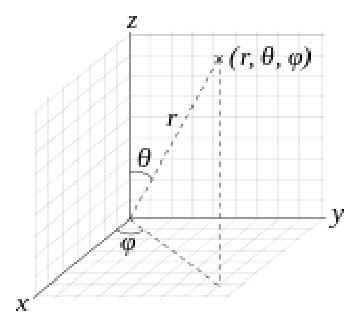
\includegraphics{157px-3D_Spherical.eps} \footnote{\ }

& 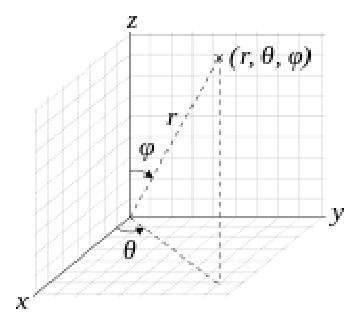
\includegraphics{157px-3D_Spherical_2.eps} \footnote{\ }
\end{tabular}
\end{center}



1-\small{`3D Spherical 2' by Dmcq - Own work. Licensed under Creative Commons Attribution-Share Alike 3.0 via Wikimedia Commons - \href{http://commons.wikimedia.org/wiki/File:3D_Spherical_2.svg\#mediaviewer/File:3D_Spherical_2.svg}{Wikipedia File} } 
\vskip0.1in
2- \small{`3D Spherical' by Andeggs - Own work. Licensed under Public domain via Wikimedia Commons - \href{http://commons.wikimedia.org/wiki/File:3D_Spherical.svg\#mediaviewer/File:3D_Spherical.svg}{Wikipedia File} }
}

\hrule
\vskip0.1in

\begin{problem} 
\marginpar{
	\thomasee{See page 893.} 
	\stewarts{See pages 827-833} 
	\larsonfive{See Larson 11.7.}
	}%
Let $P=(x,y,z)$ be a point in space. This point lies on a cylinder of radius $r$, where the cylinder has the $z$ axis as its axis of symmetry.  The height of the point is $z$ units up from the $xy$ plane. The point casts a shadow in the $xy$ plane at $Q=(x,y,0)$.  The angle between the ray $\vec{OQ}$ and the $x$-axis is $\theta$. Construct a graph in 3D of this information, and use it to develop the equations for cylindrical coordinates given above.
\end{problem}

\begin{problem}\label{derive spherical coordinates} Let 
\marginpar{
	\thomasee{See page 897.}
	\larsonfive{See Larson 11.7.}
	}% 
  $P=(x,y,z)$ be a point in space. This point lies on a sphere of
  radius $\rho$ (``rho''), where the sphere's center is at the origin
  $O=(0,0,0)$. The point casts a shadow in the $xy$ plane at
  $Q=(x,y,0)$.  The angle between the ray $\vec{OQ}$ and the $x$-axis
  is $\theta$, and is called the azimuth angle. The angle between
  the ray $\vec{OP}$ and the $z$ axis is $\phi$ (``phi''), and is
  called the inclination angle, polar angle, or zenith angle.  Construct
  a graph in 3D of this information, and use it to develop the
  equations for spherical coordinates given above.
\end{problem}

\marginpar{See the
  \href{http://en.wikipedia.org/wiki/Spherical_coordinate_system}{Wikipedia}
  or
  \href{http://mathworld.wolfram.com/SphericalCoordinates.html}{MathWorld}
  for a discussion of conventions in different disciplines.}%
	
There is some disagreement between different fields about the notation
for spherical coordinates.  In some fields (like physics), $\phi$
represents the azimuth angle and $\theta$ represents the inclination
angle.  In some fields, like geography, instead of the inclination angle, the
\emph{elevation} angle is given---the angle from the $xy$-plane (lines
of lattitude are from the elevation angle).
Additionally, sometimes the coordinates are written in a different
order.  You should always check the notation for spherical coordinates
before communicating using them.
\vskip0.1in
\hrule
\vskip0.1in
\noindent \Large After Class: \normalsize

\begin{problem}
For each curve below, set up an integral formula which would give the length, and sketch the curve. Do not worry about integrating them.  \marginpar{The reason I don't want you to actually compute the integrals is that they will get ugly really fast. Try doing one in Wolfram Alpha and see what the computer gives.}
\begin{enumerate}
\item The parabola $\vec p(t) = (t,t^2)$ for $t\in[0,3]$.
\item The ellipse $\vec e(t) = (4\cos t,5\sin t)$ for $t\in[0,2\pi]$.
\item The hyperbola $\vec h(t) = (\tan t,\sec t)$ for $t\in[-\pi/ 4,\pi/4]$.
\end{enumerate}
\end{problem}
To actually compute the integrals above and find the lengths, we would use a numerical technique to approximate the integral (something akin to adding up the areas of lots and lots of rectangles as you did in first semester calculus).

\valpo{
\begin{problem}
If you have never worked in Maple, you will want to spend some time familiarizing yourself with the program before our Lab day (keep reading if you are!). The link here takes you to a set of modules which will review several of the vector concepts we learned last week, but also introduce you to Maple. The Vector exploration contains a very nice visual on vector projections, which you should look at even if you are comfortable in Maple.
\vskip0.1in
The Connected Curriculum Project:\\
\href{https://www.math.duke.edu/education/ccp/resources/learn/index.html}{Introduction to Modules}
\vskip0.1in
\href{https://www.math.duke.edu/education/ccp/materials/mvcalc/javamaptutor/contents.html}{Maple Tutorial}
\vskip0.1in
\href{https://www.math.duke.edu/education/ccp/materials/mvcalc/vectors/index.html}{Vectors Exploration}
\end{problem}
}


%%% Local Variables: 
%%% mode: latex
%%% TeX-master: "215-problems"
%%% End: 


\chapter{Functions}
\minitoc \mtcskip
\stepcounter{unitday}

\noindent 
This unit covers the following ideas. 
\begin{enumerate}
\item Describe uses for, and construct graphs of, space curves and parametric surfaces. Find derivatives of space curves, and use this to find velocity, acceleration, and find equations of tangent lines.
\item Describe uses for, and construct graphs of, functions of several variables. For functions of the form $z=f(x,y)$, this includes both 3D surface plots and 2D level curve plots.  For functions of the form $w=f(x,y,z)$, construct plots of level surfaces.
\item Describe uses for, and construct graphs of, vector fields and transformations.
\item If you are given a description of a vector field, curve, or surface (instead of a function or parametrization), explain how to obtain a function for the vector field, or a parametrization for the curve or surface.
\end{enumerate}


\valpo{
The course objectives that will be covered in this chapter are:
\begin{enumerate}
\item identify the domain and range of a multivariable or vector-valued function
\item express curves and surfaces with parametric equations
\item compute rates of change along space curves
\item define and sketch two- or three-dimensional vector fields
\end{enumerate}
}

\clearpage

\uday
\normalsize
\begin{itemize}
\item identify the domain and range of a multivariable or vector-valued function
\item express curves and surfaces with parametric equations
\item compute rates of change along space curves
\end{itemize}

\section{Function Terminology}
A function is a set of instructions involving two sets (called the domain and codomain).  A function assigns to each element of the domain $D$ exactly one element in the codomain $R$. We'll often refer to the codomain $R$ as the target space.  We'll write $$f\colon D\to R$$ when we want to remind ourselves of the domain and target space.  In this class, we will study what happens when the domain and target space are subsets of ${\mathbb{R}}^n$ (Euclidean $n$-space).  In particular, we will study functions of the form $$f\colon {\mathbb{R}}^n\to {\mathbb{R}}^m,$$ when $m$ and $n$ are 3 or less. The value of $n$ is the dimension of the input vector (or number of inputs).  The number $m$ is the dimension of the output vector (or number of outputs).  Our goal is to understand uses for each type of function, and be able to construct graphs to represent the function.

We will focus most of our time this semester on two- and three-dimensional problems. However, many problems in the real world require a higher number of dimensions. When you hear the word ``dimension'', it does not always represent a physical dimension, such as length, width, or height.  If a quantity depends on 30 different measurements, then the problem involves 30 dimensions.  As a quick illustration, the formula for the distance between two points depends on 6 numbers, so distance is really a 6-dimensional problem.  As another example, if a piece of equipment has a color, temperature, age, and cost, we can think of that piece of equipment being represented by a point in four-dimensional space (where the coordinate axes represent color, temperature, age, and cost).

% As we introduce each type of function, we'll introduce it in the context of a somewhat realistic setting.  
% After introducing each type of surface, we'll end this chapter with an assortment of functions to practice graphing.

\begin{problem}\label{pebble problem}%
\marginpar{See 
\href{http://aleph.sagemath.org/?z=eJwrsS1LLNJQL1HXtOYqyMkv0TAz0TU00yqJM9JR0CjRMdAx0tQEAL5TCVo}{Sage}
or 
\href{http://wolfr.am/xoc07E}{Wolfram Alpha}. %http://www.wolframalpha.com/input/?i=f%28t%29%3D64-16t^2
Follow the links to Sage or Wolfram Alpha in all the problems below to see how to get the computer to graph the function.}%
A pebble falls from a 64 ft tall building.  Its height (in ft) above the ground $t$ seconds after it drops is given by the function $y=f(t)=64-16t^2$. What are $n$ and $m$ when we write this function in the form  $f\colon {\mathbb{R}}^n\to {\mathbb{R}}^m$? Construct a graph of this function.  How many dimensions do you need to graph this function?
\end{problem}

\section{Parametric Curves: $\vec f\colon \RR \to \RR^m$}

\begin{problem}\label{parametric curve in plane example}%
\marginpar{
See \href{http://aleph.sagemath.org/?z=eJwrsS1LLNJQL1HX5CpILErMTS0pykyOL8jJL9GINtJKzi_WKNHUUTDWKs7MA7JidRQ0SnQMdIy0CjI1NQFWdRJT}{Sage} or \href{http://wolfr.am/wAkR8l}{Wolfram Alpha}. %http://www.wolframalpha.com/input/?i=parametric+plot+%282+cos+t,+3+sin+t%29
See also Chapter 3 of this problem set.
	\thomasee{There's a lot more practice of this idea in 11.1. You'll also find more practice in 13.1: 1-8.}%
	\larsonfive{See also Larson 10.2.  You can also find more practice in 12.1 and 12.3.}
	\stewarts{For review on parameterizing see 10.1 and 10.2. Find more practice in 13.4:3-6 }
	}%
A horse runs around an elliptical track. Its position at time $t$ is given by the  function $\vec r(t)=(2\cos t, 3\sin t).$ We could alternatively write this as $x=2\cos t, y=3\sin t$. 
 \begin{enumerate}
  \item What are $n$ and $m$ when we write this function in the form  $\vec r\colon {\mathbb{R}}^n\to {\mathbb{R}}^m$?
  \item Construct a graph of this function. 
  \item Next to a few points on your graph, include the time $t$ at which the horse is at this point on the graph. Include an arrow for the horse's direction.
  \item How many dimensions do you need to graph this function?
 \end{enumerate}
\end{problem}


Notice in the problem above that we placed a vector symbol above the function name, as in $\vec r\colon {\mathbb{R}}^n\to {\mathbb{R}}^m$.  When the target space (codomain) is 2-dimensional or larger, we place a vector above the function name to remind us that the output is more than just a number.

In the next problem, we keep the input as just a single number $t$, but the output is now a vector in $\mathbb{R}^3$.

\begin{problem}\label{jet intro for space curves}%
\label{space curve example}%
\marginpar{
See \href{http://aleph.sagemath.org/?z=eJxL0yjRtNUw0krOLwaydBSMtIoz88CsEk2ugsSixNzUkqLM5PiCnPwSjTQdBY0SHQMdBROtgkxNTQAYOxGO}{Sage} or \href{http://www.wolframalpha.com/input/?i=parametric+plot+3D++\%282+cos+t\%2C+2+sin+t\%2C+t\%29+for+t+from+0+to+4+pi}{Wolfram Alpha}. 
	\thomasee{The text has more practice in 13.1: 9-14.}%
	\larsonfive{More practice is in Larson 12.1:9--12, 21--24, 27--32.}
	\stewarts{More practice in 13.4:7-8, 15-18}
	}%
 A jet begins spiraling upwards to gain height. The position of the jet after $t$ seconds is modeled by the equation 
$\vec r(t)=(2\cos t, 2\sin t, t).$ We could alternatively write this as $x=2\cos t,\, y=2\sin t,\, z=t$. 
\begin{enumerate}
 \item What are $n$ and $m$ when we write this function in the form  $\vec r\colon {\mathbb{R}}^n\to {\mathbb{R}}^m$? 
 \item Construct a graph of this function by picking several values of $t$ and plotting the resulting points $(2\cos t, 2\sin t, t)$. 
 \item Next to a few points on your graph, include the time $t$ at which the jet is at this point on the graph. Include an arrow for the jet's direction.
 \item  How many dimensions do you need to graph this function?
\end{enumerate}
\end{problem}

\section{Parametric Surfaces: $\vec f\colon  \RR^2 \to \RR^3$}
We now increase the number of inputs from 1 to 2.  This will allow us to graph many space curves at the same time.

\begin{problem} \label{parametric surface example}%
\marginpar{See \href{http://aleph.sagemath.org/?z=eJxL0yjRUUjUtNVI1ErOL9Yo0QTytIoz88CsEk2ugsSixNzUkqLM5PiCnPwSjTQdBaAOAx0FE62CTKASjUQdBSMgT1OTCwBCiRSf}{Sage} or \href{http://www.wolframalpha.com/input/?i=parametric+plot+3D++\%28a+cos+t\%2C+a+sin+t\%2C+t\%29+for+t+from+0+to+4+pi+and+a+from+2+to+4}{Wolfram Alpha}.
\larsonfive{More practice in Larson 15.5:1--6.}
}%
 The jet from problem \ref{jet intro for space curves} is actually accompanied by several jets flying side by side. As all the jets fly, they leave a smoke trail behind them (it's an air show). The smoke from one jet spreads outwards to mix with the neighboring jet, so that it looks like the jets are leaving a rather wide sheet of smoke behind them as they fly. The position of two of the many other jets is given by $\vec r_3(t)=(3\cos t, 3\sin t, t)$ and $\vec r_4(t)=(4\cos t,4\sin t,t)$.  A function which represents the smoke stream is $\vec r(a,t)=(a\cos t, a\sin t, t)$ for $0\leq t\leq 4\pi$ and $2\leq a\leq 4$.
 \begin{enumerate}
  \item What are $n$ and $m$ when we write the function $\vec r(a,t)=(a\cos t, a\sin t, t)$ in the form  $\vec r\colon {\mathbb{R}}^n\to {\mathbb{R}}^m$?
  \item Start by graphing the position of the three jets $\vec r(2,t)=(2\cos t, 2\sin t, t)$, $\vec r(3,t)=(3\cos t, 3\sin t, t)$ and $\vec r(4,t)=(4\cos t,4\sin t,t)$.  
  \item Let $t=0$ and graph the curve $r(a,0)=(a,0,0)$ for $a\in[2,4]$.  Then repeat this for $t=\pi/2,\pi,3\pi/2$.
  \item Describe the resulting surface.
 \end{enumerate}
\end{problem}

The function above is called a parametric surface.  Parametric surfaces are formed by joining together many parametric space curves. Most of 3D computer animation is done using parametric surfaces. Woody's entire body in {\it Toy Story} is a collection of parametric surfaces. Car companies create computer models of vehicles using parametric surfaces, and then use those parametric surfaces to study collisions. Often the mathematics behind these models is hidden in the software program, but parametric surfaces are at the heart of just about every 3D computer model.

\vskip0.1in
\hrule
\vskip0.1in
\Large
After Class:
\vskip0.1in
\normalsize



\begin{problem}%
\marginpar{
See \href{http://aleph.sagemath.org/?z=eJwNxksKgCAUBdB5q3Dmh2eQfWZuJXmIgpAodtt_Dg6crKC92g1IXIfdLoPb6aXz4JowSgz9aVCZhAJZt540aRL89hQRBqM0L_lDq7NR6h-iAhhm}{Sage} or \href{http://wolfr.am/ynm3kD}{Wolfram Alpha}. %http://www.wolframalpha.com/input/?i=parametric+plot+%283t,+64-16t^2%29
	\thomasee{The text has more practice in 13.1: 1-8.}
	\larsonfive{See also Larson 12.3.}
	\stewarts{The text has more practice in 13.4:3-6}
	}%
Consider the pebble from problem \ref{pebble problem}. The pebble's height was given by $y=64-16t^2$.  The pebble also has some horizontal velocity (it's moving at 3 ft/s to the right).  If we let the origin be the base of the 64 ft building, then the position of the pebble at time $t$ is given by $\vec r(t) = (3t, 64-16t^2)$.
 \begin{enumerate}
  \item What are $n$ and $m$ when we write this function in the form  $\vec r\colon {\mathbb{R}}^n\to {\mathbb{R}}^m$?
  \item At what time does the pebble hit the ground (the height reaches zero)?  Construct a graph of the pebble's path from when it leaves the top of the building till when it hits the ground.
  \item\marginpar{See Section~\ref{derivatives and tangent lines} and Definition~\ref{definition velocity acceleration}.}%
 Find the pebble's velocity and acceleration vectors at $t=1$? Draw these vectors on your graph with their base at the pebble's position at $t=1$. 
  \item At what speed is the pebble moving when it hits the ground?
 \end{enumerate}
\end{problem}


\begin{problem}
\marginpar{See Section~\ref{derivatives and tangent lines} and Definition~\ref{definition velocity acceleration}.}%
\marginpar{
	\thomasee{The text has more practice in 13.1: 19-22.}
	\larsonfive{More practice in Larson 12.2:23--30.} 
	\stewarts{The text has more practice in 13.2:3-8 }
	}%
 Use the same set up as problem \ref{space curve example}, namely $$\vec r(t)=(2\cos t, 2\sin t, t).$$  You'll need a graph of this function to complete this problem.
 \begin{enumerate}
  \item Find the first and second derivative of $\vec r(t)$. 
  \item Compute the velocity and acceleration vectors at $t=\pi/2$. Place these vectors on your graph with their tails at the point corresponding to $t=\pi/2$.
  \item Give an equation of the tangent line to this curve at $t=\pi/2$.
 \end{enumerate}
\end{problem}

In all the problems above, you should have noticed that in order to draw a function (provided you include arrows for direction, or use an animation to represent ``time''), you can determine how many dimensions you need to graph a function by just summing the dimensions of the domain and codomain. This is true in general.

\begin{problem*}[Optional on Parametric Surfaces]\label{second parametric surface example}%
\marginpar{See \href{http://aleph.sagemath.org/?z=eJxL0yjVUSjTtNUo1UrOL9Yo09RRKNUqzsyDsOKMNLkKEosSc1NLijKT4wty8ks00nQUQHoMdBRMgEo0ynQMdIy0CjI1NQFPyxVa}{Sage} or \href{http://wolfr.am/A90cfW}{Wolfram Alpha}.% http://www.wolframalpha.com/input/?i=parametric+plot+3d+%28u+cos+v,+u+sin+v,+u^2%29
}%
 Consider the parametric surface $\vec r(u,v)=(u\cos v, u\sin v, u^2)$ for $0\leq u\leq 3$ and $0\leq v\leq 2 \pi$.
 Construct a graph of this function. To do so, let $u$ equal a constant (such as 1, 2, 3) and then graph the resulting space curve.  Then let $v$ equal a constant (such as 0, $\pi/2$, etc.) and graph the resulting space curve until you can visualize the surface. [Hint: Think satellite dish.] 
\end{problem*}

\newpage

\uday
\normalsize
\begin{itemize}
\item identify the domain and range of a multivariable or vector-valued function
\item express curves and surfaces with parametric equations
\end{itemize}

\section{Functions of Several Variables: $f\colon \RR^n \to \RR$}

In this section we'll focus on functions of the form $f\colon \mathbb{R}^2\to\mathbb{R}^1$ and $f\colon \mathbb{R}^3\to\mathbb{R}^1$; we'll keep the output as a real number. In the next problem, you should notice that the input is a vector $(x,y)$ and the output is a number $z$. There are two ways to graph functions of this type.  The next two problems show you how. 

\begin{problem}\label{surface graph for a function of two variables}%
\marginpar{See \href{http://aleph.sagemath.org/?z=eJxL06jQqdS0tdStiDPSrYwz4irIyS8xTtFI01EAyuga6xhrAlmVEJYmADAVC84}{Sage} or 
\href{http://wolfr.am/wny0IF}{Wolfram Alpha}.%http://www.wolframalpha.com/input/?i=plot+3d+9-x^2-y^2
}%
\larsonfive{\marginpar{See Larson 13.1:33--40.}}%
 A computer chip has been disconnected from electricity and sitting in cold storage for quite some time.  The chip is connected to power, and a few moments later the temperature (in Celsius) at various points $(x,y)$ on the chip is measured. From these measurements, statistics is used to create a temperature function $z=f(x,y)$ to model the temperature at any point on the chip. Suppose that this chip's temperature function is given by the equation $z=f(x,y)=9-x^2-y^2$. We'll be creating a 3D model of this function in this problem, so you'll want to place all your graphs on the same $x,y,z$ axes.
\begin{enumerate}
 \item What is the temperature at $(0,0)$, $(1,2)$, and $(-4,3)$? \marginpar{\thomasee{See 14.1: 1-4.} \stewarts{See 14.1: 2, 7}}
 \item If you let $y=0$, construct a graph of the temperature $z=f(x,0) = 9-x^2-0^2$, or just $z=9-x^2$. In the $xz$ plane (where $y=0$) draw this upside down parabola.
 \item Now let $x=0$. Draw the resulting parabola in the $yz$ plane.
 \item Now let $z=0$. Draw the resulting curve in the $xy$ plane.
 \item Once you've drawn a curve in each of the three coordinate planes, it's useful to pick an input variable (either $x$ or $y$) and let it equal various constants. So now let $x=1$ and draw the resulting parabola in the plane $x=1$.  Then repeat this for $x=2$.
 \item Describe the shape. Add any extra features to your graph to convey the 3D image you are constructing. \marginpar{\thomasee{See 14.1: 37-48.}\stewarts{See 14.1: 23-31}}
\end{enumerate}
\end{problem}

\begin{problem}\label{cake level curves plot}%
\marginpar{See \href{http://aleph.sagemath.org/?z=eJydj81qwzAQhO9-iiWXWCCHJqbQHHTtExR6KI1RnBVWWWuNVibR21fOH_Ta2-7M7PCtqy86K7NvLoddkw-7aiJO7al2GorTtLpVZcq3SW1k4HOtqiGNVK8-EZY0pDPDyTuHEUMCSZlQgB30HBLP8RoSEIbMM_Q2gCCWdcQllAb8EwSekucgm5Wq7nq36IXoCfTg0Y9LMV8veqtf9Zvefy8qcTzaaD7ijLof7WTWP5jWT_7_FpM9IsmtFpwnMu-WBPVV73wgH_DuWpmwT1205RuzVdUvSwN0NA}{Sage} or 
\href{http://wolfr.am/wny0IF}{Wolfram Alpha}.%http://www.wolframalpha.com/input/?i=plot+3d+9-x^2-y^2
}%
\larsonfive{\marginpar{See Larson 13.1:45--56.}}%
We'll be using the same function $z=f(x,y)=9-x^2-y^2$ as the previous problem.  However, this time we'll construct a graph of the function by only studying places where the temperature is constant.  We'll create a graph in 2D of the surface (similar to a topographical map). 
 \begin{enumerate}
  \item%
\marginpar{
	\thomasee{See 14.1: 13-16 and 31-36.}
	\stewarts{See 14.1: Examples 9-13, for more practice problems 14.1:43-50}
	}%
Which points in the plane have zero temperature? Just let $z=0$ in $z=9-x^2-y^2$. Plot the corresponding points in the $xy$-plane, and write $z=0$ next to this curve. This curve is called a level curve. As long as you stay on this curve, your temperature will remain level, it will not increase nor decrease. 
  \item Which points in the plane have temperature $z=5$?  Add this level curve to your 2D plot and write $z=5$ next to it.
  \item Repeat the above for $z=8$, $z=9$, and $z=1$. What's wrong with letting $z=10$? \marginpar{\thomasee{See 14.1: 37-48.}}
  \item Using your 2D plot, construct a 3D image of the function by lifting each level curve to its corresponding height.
 \end{enumerate}
\end{problem}

\begin{definition}
 A level curve of a function $z=f(x,y)$ is a curve in the $xy$-plane found by setting the output $z$ equal to a constant. Symbolically, a level curve of $f(x,y)$ is the curve $c=f(x,y)$ for some constant $c$.  A 2D plot consisting of several level curves is called a contour plot of $z=f(x,y)$.
\end{definition}

\begin{problem}%

\marginpar{See \href{http://aleph.sagemath.org/?z=eJxL06jQqdS0rdCtjDPiKs7IL9coyMkvMU7RSNNRAErpGusYawJZlRCWpiZETXJ-Xkl-aVE8SC12lToKybmJBbbqWakl6kB2fk5-UVJikW1IUWmqTk5iUmpOMZitqQkAhh0mmg}{Sage} or 
\href{http://wolfr.am/wBOk1b}{Wolfram Alpha}. \\%http://www.wolframalpha.com/input/?i=plot+3d+x-y^2
\thomasee{More practice is in 14.1: 37-48.}}%
\larsonfive{\marginpar{See Larson 13.1:45--56.}
\stewarts{More practice is in 14.1:51-52, 55-58}}%
 Consider the function $f(x,y)=x-y^2$.
\begin{enumerate}
 \item Construct a 3D surface plot of $f$. [So just graph in 3D the curves given by $x=0$ and $y=0$ and then try setting $x$ or $y$ equal to some other constants, like $x=1$, $x=2$, $y=1$, $y=2$, etc.]
 \item Construct a contour plot of $f$. [So just graph in 2D the curves given by setting $z$ equal to a few constants, like $z=0$, $z=1$, $z=-4$, etc.]
 \item% 
\marginpar{\thomasee{See 14.1: 49-52.}}%
Which level curve passes through the point $(2,2)$?  Draw this level curve on your contour plot.
\end{enumerate}
\end{problem}

Notice that when we graphed the previous two functions (of the form $z=f(x,y)$) we could either construct a 3D surface plot, or we could reduce the dimension by 1 and construct a 2D contour plot by letting the output $z$ equal various constants. 
The next function is of the form $w=f(x,y,z)$, so it has 3 inputs and 1 output.  We could write $f\colon \mathbb{R}^3\to\mathbb{R}^1$. We would need 4 dimensions to graph this function, but graphing in 4D is not an easy task.  Instead, we'll reduce the dimension and create plots in 3D to describe the level surfaces of the function.

\vskip0.1in
\hrule
\Large
\vskip0.1in
After Class:\\
\normalsize

\begin{problem}%
\marginpar{See \href{http://aleph.sagemath.org/?z=eJwrSyzSUK_QqdSpUtfkCtEAszRtDQ0MdCvijHQrgbgqzogrM7cgJzM5syS-ICe_xDhFA67Q1tJSRwHIUdA11lEw1gSyK8FsMLMKytRUAADtWRrw}{Sage}.  \\
Wolfram Alpha currently does not support drawing level surfaces.  You could also use Mathematica or \href{http://demonstrations.wolfram.com/LevelSurfacesAndQuadraticSurfaces/}{Wolfram Demonstrations}.

\thomasee{You can access more problems on drawing level surfaces in 12.6:1-44 or 14.1:53-60.}%
\larsonfive{See Larson 11.6 and 13.1:69--74, as well as 13.1, Example 6.}
\stewarts{For more practice see 14.1:65-68 }}%
 Suppose that an explosion occurs at the origin $(0,0,0)$. Heat from the explosion starts to radiate outwards.  Suppose that a few moments after the explosion, the temperature at any point in space is given by $w=T(x,y,z)=100-x^2-y^2-z^2.$ 
\begin{enumerate}
 \item Which points in space have a temperature of 99?  To answer this, replace $T(x,y,z)$ by $99$ to get $99=100-x^2-y^2-z^2$. Use algebra to simplify this to $x^2+y^2+z^2=1$.  Draw this object.
 \item Which points in space have a temperature of 96? of 84? Draw the surfaces. 
 \item What is your temperature at $(3,0,-4)$? Draw the level surface that passes through $(3,0,-4)$.
\item The 4 surfaces you drew above are called level surfaces. If you walk along a level surface, what happens to your temperature?
 \item As you move outwards, away from the origin, what happens to your temperature?
\end{enumerate}
\end{problem}

\note{Talk about graphing functions with 4 or more variables.  Show the class \href{http://www.osirix-viewer.com/}{OsiriX} as an example of graphing a 4d function (where opacity is the density of material.  Also, practice sliding a plane through a 3d object to get an idea of what the contour plots are telling us. One example could be a play-do object, and actually taking slices of it.}

\begin{problem}
\marginpar{See \href{http://aleph.sagemath.org/?z=eJwrSyzSUK_QqdSpUtfkStMAszRtK-KMtKvijLgycwtyMpMzS-ILcvJLjFM04ApsTXQUgGwFXWMdBWNNILsSzAYzq6BMTQUAEvYY4A}{Sage}.%

\larsonfive{See Larson 11.6:7--16.}}%
Consider the function $w=f(x,y,z)=x^2+z^2$. This function has an input $y$, but notice that changing the input $y$ does not change the output of the function.
 \begin{enumerate}
  \item Draw a graph of the level surface $w=4$. [When $y=0$ you can draw one curve.  When $y=1$, you should draw the same curve.  When $y=2$, again you draw the same curve.  This kind of graph is called a cylinder, and is important in manufacturing where you extrude an object through a hole.]
  \item Graph the surface $9=x^2+z^2$ (so the level surface $w=9$).
  \item Graph the surface $16=x^2+z^2$.
 \end{enumerate}
\end{problem}

Most of our examples of function of the form $w=f(x,y,z)$ can be drawn by using our knowledge about conic sections. We can graph ellipses and hyperbolas if there are only two variables. So the key idea is to set one of the variables equal to a constant and then graph the resulting curve.  Repeat this with a few variables and a few constants, and you'll know what the surface is. Sometimes when you set a specific variable equal to a constant, you'll get an ellipse. If this occurs, try setting that variable equal to other constants, as ellipses are generally the easiest curves to draw.

\begin{problem*}[Optional: More Surface Practice]
\marginpar{See \href{http://aleph.sagemath.org/?z=eJwrSyzSUK_QqdSpUtfkStMAszRtK-KMdCvjjLSr4oy4MnMLcjKTM0viC3LyS4xTNOCKbA11FIBsBV1jHQVjTSC7EswGM6ugTE0FAIXAGhM}{Sage}.

	\thomasee{Remember you can find more practice in 12.6:1-44 or 14.1: 53-64.}%
	\larsonfive{See Larson 11.6 and 13.1:69--74, as well as 13.1, Example 6.}
	\stewarts{Remember you can find more practice in 14.1:65-68}
	}%

Consider the function $w=f(x,y,z)=x^2-y^2+z^2$.\marginparbmw{We'll have a few people present this problem.}
 \begin{enumerate}
  \item Draw a graph of the level surface $w=1$. [You need to graph $1=x^2-y^2+z^2$. Let $x=0$ and draw the resulting curve. Then let $y=0$ and draw the resulting curve. Let either $x$ or $y$ equal some more constants (whichever gave you an ellipse), and then draw the resulting ellipses.]  
  \item Graph the level surface $w=4$. [Divide both sides by $4$ (to get a 1 on the left) and the repeat the previous part.]
  \item Graph the level surface $w=-1$. [Try dividing both sides by a number to get a 1 on the left. If $y=0$ doesn't help, try $y=1$ or $y=2$.]
  \item Graph the level surface that passes through the point $(3,5,4)$. [Hint: what is $f(3,5,4)$?]
 \end{enumerate}
\end{problem*}

\uday
\normalsize
\begin{itemize}
\item identify the domain and range of a multivariable or vector-valued function
\item define and sketch two- or three- dimensional vector fields
\end{itemize}

\subsection{Vector Fields and Transformations: $\vec f\colon \RR^n\to\RR^n$}

We've covered the following types of functions in the problems above.
\begin{itemize}
 \item $y=f(x)$ or $f\colon \mathbb{R}\to\mathbb{R}$ (functions of a single variable)
 \item $\vec r(t)=(x,y)$ or $f\colon \mathbb{R}\to\mathbb{R}^2$ (parametric curves)
 \item $\vec r(t)=(x,y,z)$ or $f\colon \mathbb{R}\to\mathbb{R}^3$ (space curves)
 \item $\vec r(u,v)=(x,y,z)$ or $f\colon \mathbb{R}^2\to\mathbb{R}^3$ (parametric surfaces)
 \item $z=f(x,y)$ or $f\colon \mathbb{R}^2\to\mathbb{R}$ (functions of two variables)
 \item $z=f(x,y,z)$ or $f\colon \mathbb{R}^3\to\mathbb{R}$ (functions of three variables)
\end{itemize}
We will finish this section by considering vector fields and transformations. 
\begin{itemize}
 \item $\vec F(x,y)=(M,N)$ or $f\colon \mathbb{R}^2\to\mathbb{R}^2$ (vector fields in the plane)
 \item $\vec F(x,y,z)=(M,N,P)$ or $f\colon \mathbb{R}^3\to\mathbb{R}^3$ (vector fields in space)
 \item $\vec T(u,v)=(x,y)$ or $f\colon \mathbb{R}^2\to\mathbb{R}^2$ (2D transformation)
 \item $\vec T(u,v,w)=(x,y,z)$ or $f\colon \mathbb{R}^3\to\mathbb{R}^3$ (3D transformation)
\end{itemize}
Notice that in all cases, the dimension of the input and output are the same. The difference between vector fields and transformations has to do with the application. We've already seen examples of transformations with polar, cylindrical, and spherical coordinates.

\begin{problem}\label{graphing spherical coordinates}%
\marginpar{Recall that $\phi$ (``phi'') is the angle down from the $z$ axis, $\theta$ (``theta'') is the angle counterclockwise from the $x$-axis in the $xy$-plane, and $\rho$ (``rho'') is the distance from the origin. Review problem \ref{derive spherical coordinates} if you need a refresher.}%
\larsonfive{\marginpar{See Larson 11.7:89--94, 111--114.}}%

Consider the spherical coordinates transformation as defined in 
\stewarts{$$\vec T(\rho,\phi,\theta)=(\rho\sin\phi\cos\theta,\rho\sin\phi\sin\theta,\rho\cos\phi),$$}
\bmw{$$\vec T(\rho,\phi,\theta)=(\rho\sin\phi\cos\theta,\rho\sin\phi\sin\theta,\rho\cos\phi),$$ }
\larsonfive{$$\vec T(\rho,\theta,\phi)=(\rho\sin\phi\cos\theta,\rho\sin\phi\sin\theta,\rho\cos\phi),$$ }
which could also be written as 
\begin{align*}
x&=\rho\sin\phi\cos\theta\\y&=\rho\sin\phi\sin\theta\\z&=\rho\cos\phi. 
\end{align*}
  Graphing this transformation requires $3+3=6$ dimensions. In this problem we'll construct parts of this graph by graphing various surfaces. We did something similar for the polar coordinate transformation in problem \ref{polar coordinate transformation graph}. 
\begin{enumerate}
 \item% 
   \marginpar{See \href{http://aleph.sagemath.org/?z=eJxVjsEKhDAMRO9-xeCpKTmId__C-1JEaEBtaPP_bLMirLe8ecOQNdRcGJqFYXm3RFjgWWxyhR5T3EoLt2K8hB__wosuaNAql2FcfWiZCdJGxkODpprO3apsHz2KhUcw7jnGxJijiie_zzp3oi_jZjWn}{Sage} or 
\href{http://www.wolframalpha.com/input/?i=parametric+plot+3d+\%282+sin+phi+cos+theta\%2C+2+sin+phi+sin+theta\%2C+2+cos+phi\%29}{Wolfram Alpha}.}%
Let $\rho=2$ and graph the resulting surface.  What do you get if $\rho = 3$?
 \item % 
\marginpar{See 
\href{http://aleph.sagemath.org/?z=eJxVjrEKwzAMRPd8xZHJMioNTdf8RfZiQsCCNha2_p9WyeJuuveOQ2uouTA0C8PybomwwFlscoQfpriVFi7F-BN-9MKLLmjQKodhXD0uKvcnQdrI6MCgqabPblW2l76Lhc4xrl3GxHhEFSfnn7eZMRN9AfBbOD8}{Sage} or 
\href{http://www.wolframalpha.com/input/?i=parametric+plot+3d+\%28rho+sin+\%28pi\%2F4\%29+cos+theta\%2C+rho+sin+\%28pi\%2F4\%29+sin+theta\%2C+rho+cos+\%28pi\%2F4\%29\%29+}{Wolfram Alpha}.
}%
Let $\phi=\pi/4$ and graph the resulting surface.  What do you get if $\phi=\pi/2$?
 \item Let $\theta=\pi/4$ and graph the resulting surface.  What do you get if $\theta=\pi/2$?
\end{enumerate}

\end{problem}

We now explore a vector field example.

\begin{problem}%
\marginpar{See 
\href{http://aleph.sagemath.org/?z=eJxz06jQqdRUsFXQMNKq0K7UqdA20qrU5CrIyS-JL0tNLskvik_LTM1J0XDTUQAq1TU00DE00ASyK2FsTQCKaxIN}{Sage} or
\href{http://wolfr.am/y4gIgX}{Wolfram Alpha}. % http://www.wolframalpha.com/input/?i=plot+a+vector+field&f1={2x%2By%2Cx%2B2y}&x=6&y=7&f=VectorPlot.vectorfunction_{2x%2By%2Cx%2B2y}&f2=x&f=VectorPlot.vectorplotvariable1_x&f3=-10&f=VectorPlot.vectorplotlowerrange1_-10&f4=10&f=VectorPlot.vectorplotupperrange1_10&f5=y&f=VectorPlot.vectorplotvariable2_y&f6=-10&f=VectorPlot.vectorplotlowerrange2_-10&f7=10&f=VectorPlot.vectorplotupperrange2_10
The computer will shrink the largest vector down in size so it does not overlap any of the others, and then reduce the size of all the vectors accordingly. 

\thomasee{See 16.2: 39-44 for more practice.}%
\larsonfive{See Larson 15.1:1--19.}
\stewarts{See 16.1: 1-14 for more practice.}
}%
 Consider the vector field $\vec F(x,y)=(2x+y,x+2y)$.  In this problem, you will construct a graph of this vector field by hand.
\begin{enumerate}
 \item Compute $\vec F(1,0)$. Then draw the vector $F(1,0)$ with its base at $(1,0)$.
 \item Compute $\vec F(1,1)$. Then draw the vector $F(1,1)$ with its base at $(1,1)$.
 \item Repeat the above process for the points $(0,1)$, $(-1,1)$, $(-1,0)$, $(-1,-1)$, $(0,-1),$ and $(1,-1)$. Remember, at each point draw a vector.  
\end{enumerate}
\end{problem}


\note{Talk about vector field visualization, mention line integral convolutions and streamline plots.  Show Sage or mathematica doing these sorts of plots.}

\href{http://aleph.sagemath.org/?z=eJxz06jQqdSp0lSwVdAA0joVmlwFOfkl8WWpySX5RfFpmak5KcYpGm46CkCFusY6xpo6IIUQlkYVhKEJAOGFExs}{Sage} can also help us visualize 3d vector fields, like $\vec F(x,y,z)=(y,z,x)$. \note{use 3d glasses and Sage/JMol's ability to render for 3d glasses to \emph{really} see this vector field!}

\section{Constructing Functions}
We now know how to draw a vector field provided someone tells us the equation. How do we obtain an equation of a vector field? The following problem will help you develop the gravitational vector field.

\begin{problem}[Radial fields]
\marginpar{Use \href{http://aleph.sagemath.org/?z=eJxz06jQqdSp0lSwVdAA0joVmlwFOfkl8WWpySX5RfFpmak5KcYpGm46CkCFusY6xpo6IIUQlkYVhKEJAOGFExs}{Sage} to plot your vector fields.  

\thomasee{See 16.2: 39-44 for more practice.}%
\larsonfive{See Larson 15.1:1--19.}}%
Do the following:
\begin{enumerate}
 \item Let $P=(x,y,z)$ be a point in space.  At the point $P$, let $\vec F(x,y,z)$ be the vector which points from $P$ to the origin.  Give a formula for $\vec F(x,y,z)$.
 \item Give an equation of the vector field where at each point $P$ in the plane, the vector $\vec F_2(P)$ is a unit vector that points towards the origin.
 \item Give an equation of the vector field where at each point $P$ in the plane, the vector $\vec F_3(P)$ is a vector of length 7 that points towards the origin.
% \item Give an equation of the vector field where at each point $P$ in the plane, the vector $\vec G(P)$ points towards the origin, and has a magnitude equal to $1/d^2$ where $d$ is the distance to the origin.
\end{enumerate}
\end{problem}

If someone gives us parametric equations for a curve in the plane, we know how to draw the curve.  How do we obtain parametric equations of a given curve? In problem \ref{parametric curve in plane example}, we were given the parametric equation for the path of a horse, namely $x=2\cos t, y=3 \sin t$ or $\vec r(t)=(2\cos t,3\sin t)$. From those equations, we drew the path of the horse, and could have written a Cartesian equation for the path. How do we work this in reverse, namely if we had only been given the ellipse $\ds\frac{x^2}{4}+\frac{y^2}{9}=1$, could we have obtained parametric equations $\vec r(t)=(x(t),y(t))$ for the curve?

%\begin{problem}\label{parameterizing plane curves}
%\marginpar{Use \href{http://aleph.sagemath.org/?z=eJwrsS1LLNJQL1HX5CpILErMTS0pykyOL8jJL9GINtJKzi_WKNHUUTDWKs7MA7JidRQ0SnQMdIy0CjI1NQFWdRJT}{Sage} or \href{http://wolfr.am/wAkR8l}{Wolfram Alpha} %http://www.wolframalpha.com/input/?i=parametric+plot+%282+cos+t,+3+sin+t%29
%to visualize your parameterizations.
%}%
 %Give a parametrization of the top half of the ellipse $\ds\frac{x^2}{a^2}+\frac{y^2}{b^2}=1$, so $y\geq 0$.
 %You can write your parametrization in the vector form $\vec r(t)=(?,?)$, or in the parametric form $x=?,\ y=?$. 
 %Include bounds for $t$. 
% [Hint: Review \ref{parametric curve in plane example}.]
%\end{problem}


\begin{problem}
 Give a parametrization of the straight line from $(a,0)$ to $(0,b)$. 
 You can write your parametrization in the vector form $\vec r(t)=(?,?)$, or in the parametric form $x=?,\ y=?$. 
 Remember to include bounds for $t$. [Hint: Review \ref{first line between two points} and \ref{line equation to refer to}.]
\end{problem}

%\hrule
\newpage
\Large
After Class:\\
\normalsize

\begin{problem}[Vector Fields: The Spin field]
\marginpar{Use the links above to see the computer plot this.  

\thomasee{See 16.2: 39-44 for more practice.}%
\larsonfive{See Larson 15.1:1--19.}
\stewarts{See 16.1: 1-14 for more practice.}}%
 Consider the vector field $\vec F(x,y)=(-y,x)$. Construct a graph of this vector field. Remember, the key to plotting a vector field is ``at the point $(x,y)$, draw the vector $\vec F(x,y)$ with its base at $(x,y)$.''  Plot at least 8 vectors (a few in each quadrant), so we can see what this field is doing.
\end{problem}

\begin{problem}
 Give a parametrization of the parabola $y=x^2$ from $(-1,1)$ to $(2,4)$. 
 Remember the bounds for $t$.
\end{problem}


\begin{problem}
 Give a parametrization of the function $y=f(x)$ for $x\in[a,b]$.
 You can write your parametrization in the vector form $\vec r(t)=(?,?)$, or in the parametric form $x=?,\ y=?$. 
 Include bounds for $t$.
\end{problem}

\newpage

\uday
\normalsize
\begin{itemize}
\item identify the domain and range of a multivariable or vector-valued function
\item express curves and surfaces with parametric equations
\end{itemize}

\vskip0.2in
%%%%%%%%%%%%%%%%%%%%%%%%%%%%%%%%%%%%%%%
%%%%%%%%%%%%%%%%%%%%%%%%%%%%%%%%%%%%%%%
%%%%%%%%%%%%%%%%%%%%%%%%%%%%%%%%%%%%%%%
\note{Idea.  They did the problem below already when drawing spherical coordinates.  They already practiced removing a variable.  I somehow need to make that connect to this part. How to do it, I'm not sure. Think about it, and try something different next time.}
%%%%%%%%%%%%%%%%%%%%%%%%%%%%%%%%%%%%%%%
%%%%%%%%%%%%%%%%%%%%%%%%%%%%%%%%%%%%%%%
%%%%%%%%%%%%%%%%%%%%%%%%%%%%%%%%%%%%%%%
If someone gives us parametric equations for a surface, we can draw the surface. This is what we did in problems \ref{parametric surface example} and \ref{second parametric surface example}. 
How do we work backwards and obtain parametric equations for a given surface?
This requires that we write an equation for $x$, $y$, and $z$ in terms of two input variables (see \ref{parametric surface example} and \ref{second parametric surface example} for examples). 
In vector form, we need a function $\vec r\colon \mathbb{R}^2\to\mathbb{R}^3$. 
We can often use a coordinate transformation $\vec T\colon \mathbb{R}^3\to\mathbb{R}^3$ to obtain a parametrization of a surface. 
The next three problems show how to do this.   
\begin{problem}\label{3d parametric plot}
\marginpar{Use \href{http://aleph.sagemath.org/?z=eJwL0ajQqdSp0lSwVYCyuAqKMvNKFJRCNKpsK7QrNRUyi5V0FGA8roLEosTc1JKizOT4gpz8Eg2YhA5Iv66xjjGIVQlhaQIALhka5w}{Sage} or
\href{http://wolfr.am/zk2KTu}{Wolfram Alpha} %http://www.wolframalpha.com/input/?i=parametric+plot+3d+%28x%2Cy%2Cx%2By%29
to plot your parametrization.  

	\thomasee{See 16.5: 1-16 for more practice.}%
	\larsonfive{See Larson 15.5:21--30 and 15.5, Example 3.}
	\stewarts{See section 16.6 for more examples}
	}%
 Consider the surface $z=9-x^2-y^2$ plotted in problem \ref{surface graph for a function of two variables}.
\begin{enumerate}
 \item 
Using the rectangular coordinate transformation $\vec T(x,y,z)=(x,y,z)$, give a parametrization $\vec r\colon \mathbb{R}^2\to\mathbb{R}^3$ of the surface. 

This is the same as saying $$x=x, y=y, z=?.$$
[Hint: Use the surface equation to eliminate the input variable $z$ in $T$.]

 \item What bounds must you place on $x$ and $y$ to obtain the portion of the surface above the plane $z=0$?
 \item If $z=f(x,y)$ is any surface, give a parametrization of the surface (i.e., $x=?, y=?, z=?$ or $\vec r (?,?)=(?,?,?)$.)
\end{enumerate}

\end{problem}
\begin{problem}%
\marginpar{Use \href{http://aleph.sagemath.org}{Sage} or \href{http://wolframalpha.com}{Wolfram Alpha} to plot your parametrization with your bounds (see \ref{3d parametric plot} for examples).  

	\thomasee{See 16.5: 1-16 for more practice.}%
	\larsonfive{See Larson 15.5:1--10}
	}%
 Again consider the surface $z=9-x^2-y^2$.
\begin{enumerate}
 \item
Using cylindrical coordinates, $\vec T(r,\theta,z) = (r\cos \theta, r\sin\theta, z)$, obtain a parametrization $\vec r(r,\theta)=(?,?,?)$ of the surface using the input variables $r$ and $\theta$. In other words, if we let $x=r\cos \theta, y=r\sin\theta, z=z$, and writing $z=9-x^2-y^2$ in terms of $r$ and $\theta$.
 \item What bounds must you place on $r$ and $\theta$ to obtain the portion of the surface above the plane $z=0$?
\end{enumerate}

\end{problem}


\begin{problem}%
\marginpar{
	We did very similar things in problem \ref{graphing spherical coordinates}.

	\thomasee{See 16.5: 1-16 for more practice.}
	\larsonfive{See Larson 15.5:1--10}
	}%

Recall the spherical coordinate transformation as given in 
\stewarts{$$\vec T(\rho,\phi,\theta) = (\rho\sin\phi\cos \theta, \rho\sin\phi\sin \theta,\rho \cos \phi).$$}
\bmw{$$\vec T(\rho,\phi,\theta) = (\rho\sin\phi\cos \theta, \rho\sin\phi\sin \theta,\rho \cos \phi).$$ }%
\larsonfive{$$\vec T(\rho,\theta, \phi) = (\rho\sin\phi\cos \theta, \rho\sin\phi\sin \theta,\rho \cos \phi).$$}%
This is a function of the form $\vec T\colon \mathbb{R}^3\to\mathbb{R}^3$.  If we hold one of the three inputs constant, then we have a function of the form $\vec r\colon \mathbb{R}^2\to\mathbb{R}^3$, which is a parametric surface.
\begin{enumerate}
 \item \marginpar{Use \href{http://aleph.sagemath.org}{Sage} or \href{http://www.wolframalpha.com/}{Wolfram Alpha} to plot each parametrization (see \ref{3d parametric plot} for examples).}%
Give a parametrization of the sphere of radius 2, using $\phi$ and $\theta$ as your input variables. 
 \item What bounds should you place on $\phi$ and $\theta$ if you want to hit each point on the sphere exactly once?
 \item What bounds should you place on $\phi$ and $\theta$ if you only want the portion of the sphere above the plane $z=1$?
\end{enumerate}
\end{problem}

\newpage

\Large
Bonus Questions:
\vskip0.1in
\normalsize

Sometimes you'll have to invent your own coordinate system when constructing parametric equations for a surface.  If you notice that there are lots of circles parallel to one of the coordinate planes, try using a modified version of cylindrical coordinates. Instead of circles in the $xy$ plane ($x=r\cos\theta,y=r\sin\theta,z=z$), maybe you need circles in the $yz$-plane ($x=x,y=r\sin\theta,z=r\sin\theta$) or the $xz$ plane.  Just look for lots of circles, and then construct your parametrization accordingly.
\begin{problem}
\marginpar{\larsonfive{See Larson 15.5:21--30.}}%
Find parametric equations for the surface $x^2+z^2=9$. [Hint: read the paragraph above.]  
\begin{enumerate}
 \item\marginpar{Use \href{http://aleph.sagemath.org}{Sage} or \href{http://www.wolframalpha.com/}{Wolfram Alpha} to plot each parametrization  (see \ref{3d parametric plot} for examples).}%
 What bounds should you use to obtain the portion of the surface between $y=-2$ and $y=3$?
 \item What bounds should you use to obtain the portion of the surface above $z=0$?
 \item What bounds should you use to obtain the portion of the surface with $x\geq 0$ and $y\in[2,5]$?
\end{enumerate}
\end{problem}

\begin{problem}
 Construct a graph of the surface $z = x^2-y^2$.  Do so in 2 ways.  (1) Construct a 3D surface plot.  (2) Construct a contour plot, which is a graph with several level curves. Which level curve passes through the point $(3,4)$? 
 Use Wolfram Alpha to know if you're right.  Just type ``plot z=x\^2-y\^2.''
\end{problem}

\begin{problem}
Construct a plot of the vector field $$\vec F(x,y) = (x+y, -x+1)$$ by graphing the field at many integer points around the origin (I generally like to get the 8 integer points around the origin, and then a few more).
Then explain how to modify your graph to obtain a plot of the vector field $$\hat F(x,y) = \frac{(x+y, -x+1)}{\sqrt{(x+y)^2+(1-x)^2}}.$$ 
\end{problem}

\clearpage

%%% Local Variables: 
%%% mode: latex
%%% TeX-master: "215-problems"
%%% End: 

%\wrapup
%
%
%
\chapter{Derivatives}
%\note{Having them come up with how to generalize differential notation to higher dimensions, and then use differential notation as well, was too much. Perhaps I need one more problem right shortly after \ref{derive matrix derivative}.  In \ref{derive matrix derivative}, the students are taking differential notation and from it writing a matrix (it's how they discover the derivative).  What I need is to have the students write differential notation in terms of a matrix.  Perhaps this would be best after the next problem.  We're already finished with derivatives, so I'll put a note to myself to polish this up next semester. See my notes at the end as well.\\(From Jason) I added a pretty extensive problem having them practice differential notation.  We'll see if that helps them to get familiar with the ideas before moving to matrix multiplication.}


%There's a link in this file to dropbox.  Rather than have to hunt for it later, here it is.
\newcommand{\derivativehomeworklink}[1]{\href{http://db.tt/cSeKG8XO}{#1}}%
%
%
\noindent 
This unit covers the following ideas. In preparation for the quiz and exam, make sure you have a lesson plan containing examples that explain and illustrate the following concepts.  
\begin{enumerate}
\item Find limits, and be able to explain when a function does not have a limit by considering different approaches.
\item Compute partial derivatives. Explain how to obtain the total derivative from the partial derivatives (using a matrix).
\item Find equations of tangent lines and tangent planes to surfaces. We'll do this three ways.
\item Find derivatives of composite functions, using the chain rule (matrix multiplication).
\end{enumerate}
You'll have a chance to teach your examples to your peers prior to the exam.





\section{Limits}
In the previous chapter, we learned how to describe lots of different functions. In first-semester calculus, after reviewing functions, you learned how to compute limits of functions, and then used those ideas to develop the derivative of a function. The exact same process is used to develop calculus in high dimensions. One glitch that will prevent us from developing calculus this way in high dimensions is the epsilon-delta definition of a limit.  We'll review it briefly.  Those of you who want to pursue further mathematical study will spend much more time on this topic in future courses. 

In first-semester calculus, you learned how to compute limits of functions. Here's the formal epsilon-delta definition of a limit. 
\begin{definition}
 Let $f:\R\to\R$ be a function.
 We write $\ds \lim_{x\to c} f(x)=L$ if and only if for every $\epsilon>0$, there exists a $\delta>0$ such that $0<|x-c|<\delta$ implies $|f(x)-L|<\epsilon$.
\end{definition}
 We're looking at this formal definition here because we can compare it with the formal definition of limits in higher dimensions. The only difference is that we just put vector symbols above the input $x$ and the output $f(x)$.
\begin{definition}
 Let $\vec f:\R^n\to\R^m$ be a function.
 We write $\ds \lim_{\vec x\to \vec c} \vec f(\vec x)=\vec L$ if and only if for every $\epsilon>0$, there exists a $\delta>0$ such that $0<|\vec x-\vec c|<\delta$ implies $|\vec f(\vec x)-\vec L|<\epsilon$.
\end{definition}
We'll find that throughout this course, the key difference between first-semester calculus and multivariate calculus is that we replace the input $x$ and output $y$ of functions with the vectors $\vec x$ and $\vec y$. 
 
\begin{problem}
 For the function $f(x,y)=z$, we can write $f$ in the vector notation $\vec y=\vec f(\vec x)$ if we let $\vec x=(x,y)$ and $\vec y=(z)$. Notice that $\vec x$ is a vector of inputs, and $\vec y$ is a vector of outputs. 
 For each of the functions below, state what $\vec x$ and $\vec y$ should be so that the function can be written in the form $\vec y = \vec f (\vec x)$. \marginpar{The point to this problem is to help you learn to recognize the dimensions of the domain and codomain of the function.  If we write $\vec f:\R^n\to \R^m$, then $\vec x$ is a vector in $\R^n$ with $n$ components, and $\vec y$ is a vector in $\R^m$ with $m$ components.}  
\begin{enumerate}
 \item $f(x,y,z)=w$
 \item $\vec r(t)=(x,y,z)$
 \item $\vec r(u,v)=(x,y,z)$
 \item $\vec F(x,y)=(M,N)$
 \item $\vec F(\rho,\phi,\theta)=(x,y,z)$
\end{enumerate}
\end{problem}


You learned to work with limits in first-semester calculus without needing the formal definitions above. Many of those techniques apply in higher dimensions. 
The following problem has you review some of these technique, and apply them in higher dimensions.
\begin{problem}\marginpar{\bmw{See 14.2: 1-30 for more practice.}}%
 Do these problems without using L'Hopital's rule.
%, as there is not a good substitute for L'Hopital's rule in higher dimensions. \note{check this.}
\begin{enumerate}
 \item Compute $\ds \lim_{x\to 2} x^2-3x+5$ and then $\ds\lim_{(x,y)\to (2,1)} 9-x^2-y^2$.
 \item Compute $\ds\lim_{x\to 3}\frac{x^2-9}{x-3}$ and then $\ds\lim_{(x,y)\to (4,4)} \frac{x-y}{x^2-y^2}$.
 \item Explain why $\ds\lim_{x\to 0}\frac{x}{|x|}$ does not exist. [Hint: graph the function.]
\end{enumerate}
\end{problem}



In first semester calculus, we can show that a limit does or does not exist by considering what happens from the left, and comparing it to what happens on the right.  You probably used the following theorem extensively. 
\begin{quote}
 If $y=f(x)$ is a function defined on some open interval containing $c$, then $\ds\lim_{x\to c}f(x)$ exists if and only if  $\ds\lim_{x\to c^-}f(x) = \ds\lim_{x\to c^+}f(x)$.
\end{quote}
 A limit exists precisely when the limits from every direction exists, and all directional limits are equal. In first-semester calculus, this required that you check two directions (left and right). This theorem generalizes to higher dimensions, but it becomes much more difficult to apply. 

\begin{example}
 Consider the function $\ds f(x,y)=\frac{x^2-y^2}{x^2+y^2}$.
Our goal is to determine if the function has a limit at the origin $(0,0)$. We can approach the origin along many different lines.

One line through the origin is the line $y=2x$. If we stay on this line, then we can replace each $y$ with $2x$ and then compute
$$\ds\lim_{\text{\footnotesize $\begin{array}{c}(x,y)\to(0,0)\\ y=2x\end{array}$}}\frac{x^2-y^2}{x^2+y^2} 
= \lim_{x\to 0} \frac{x^2-(2x)^2}{x^2+(2x)^2}
= \lim_{x\to 0} \frac{-3x^2}{5x^2}
= \lim_{x\to 0} \frac{-3}{5}
=\frac{-3}{5}.$$
This means that if we approach the origin along the line $y=2x$, we will have a height of $-3/5$ when we arrive at the origin.
\end{example}
If the function $\ds f(x,y)=\frac{x^2-y^2}{x^2+y^2}$ has a limit at the origin, the previous problem suggests that limit will be $-3/5$.
\begin{problem}
 Please read the previous example. Recall that we are looking for the limit of the function $\ds f(x,y)=\frac{x^2-y^2}{x^2+y^2}$ at the origin (0,0). 
\marginpar{You may want to look at a graph in 
\href{https://sagecell.sagemath.org/?z=eJxL06jQqdS01aiIM9KtjDPS1AextEEsXq7k_LyS_NKi-IKc_BKNNB2gSl1jHWNNHY1KKCM5Pye_KCmxyDakqDRVJzk3scBWPSu1RF1Trzgjv1wDaARIq3EKNs2aALkvIzE=}{Sage} or \href{http://wolfr.am/ioCqzX}{Wolfram Alpha} (try using the ``contour lines'' option). %http://www.wolframalpha.com/input/?i=plot+%28x%5E2-y%5E2%29%2F%28x%5E2%2By%5E2%29
 As you compute each limit, make sure you understand what that limit means in the graph.}
Our goal is to determine if the function has a limit at the origin $(0,0)$.
\begin{enumerate}
 \item In the $xy$-plane, how many lines pass through the origin $(0,0)$? Give an equation a line other than $y=2x$ that passes through the origin.  Then compute $$\ds\lim_{\text{\footnotesize $\begin{array}{c}(x,y)\to(0,0)\\ \text{your line}\end{array}$}}\frac{x^2-y^2}{x^2+y^2}
= \lim_{x\to 0} \frac{x^2-(?)^2}{x^2+(?)^2}=\ldots.$$
 \item Give another equation a line that passes through the origin.  Then compute $$\ds\lim_{\text{\footnotesize $\begin{array}{c}(x,y)\to(0,0)\\ \text{your line}\end{array}$}}\frac{x^2-y^2}{x^2+y^2}.$$
 \item Does this function have a limit at $(0,0)$? Explain. \marginpar{\bmw{See 14.2: 41-50 for more practice.}\larsonfive{See Larson 13.2:23--36 and example 4 for more practice.}}%
\end{enumerate}
\end{problem}


The theorem from first-semester calculus generalizes as follows.
\begin{quote}
 If $\vec y=\vec f(\vec x)$ is a function defined on some open region containing $\vec c$, then $\ds\lim_{\vec x\to \vec c}\vec f(\vec x)$ exists if and only if the limit exists along every possible approach to $\vec c$ and all these limits are equal.
\end{quote}
There's a fundamental problem with using this theorem to check if a limit exists. Once the domain is 2-dimensional or higher, there are infinitely many ways to approach a point. There is no longer just a left and right side. To prove a limit exists, you must check infinitely many cases---that takes a \emph{really} long time.  The real power to this theorem is it allows to show that a limit does not exist.  All we have to do is find two approaches with different limits.



\begin{problem}
\marginpar{See \href{https://sagecell.sagemath.org/?z=eJyVVF1r2zAUfc-vuKQFy7PS2QndoCBY2dtgMFjfShtubLnW6lhCUlqrv37XlvOxtdtYEoKlc3TOufcKn50BfNFNBzcWn5Tj8FU5N_yMUfBZt618kBy-G6u6B1jmRTGbPaFlSc9Dks4-qc5Li6WfVbKGNauF6szOrze6Z7SDu9YL1r8L6XvW3y-zcL9MUz6D8WP8W-Sc5ymHFjeyFfNvmvSv4JyRWyrO5xyeVeUbUeQHFTTGaiyb4g2xRX9Qup5oUJBc-LvU8g0pSv9aa_laa5JKr8aHPuchF8aPi6GFHhq_bVlyDW5naywl7eoNbtoADTpAaNVWeUAPviFsKB9UPSysBOWg0wTS2aqSHZQNdg-0TU-61TayLpJ0MIv2diDQAHifLwr6y4oYMExAoHgEhAOwTyVIsvN6Z9em1Z7VPErx6SQvt2hE8kP6hI_eG7Tixu4IiMecuJx6MRa0jpWIWBFjY1_SeFQkVlYJd-pFilXOX7StpBWreLqmsnCokB3mzI9zmrp8EjwTamtaVQ6WQ_CwwH30ffLouWmxfEymohv9zE5yZpNYRLGXTqC1xGFR6ra44-M13a-XcZ1mEy2fzEYi3ebjxsA85eV8UURCzov0aJgJL3u_qti8p9t19Mkuislqj4f5r_oj4wR_me_lCZkcjBiaQ2j9W3NAG6TeBZFffOADJzbEiY-XFJpy_d9QTCYMWtxKb1UZB0J3EXnNgkB6EcDhVm1VJ449ozX24tgy36jysZPOidUf52f-qYLOyNKvLXqlxW3B6XuXzn4C8NyNiQ}{Sage}.}%
\marginpar{\bmw{See 14.2: 41-50 for more practice.}\larsonfive{See Larson 13.2:9--36 for more practice.}}%
 Consider the function $\ds f(x,y) = \frac{xy}{x^2+y^2}$.  Does this function have a limit at $(0,0)$?  

 \begin{enumerate}
 \item Examine the function at $(0,0)$ by considering the limit as you approach the origin along several lines. 
 \item Convert $\frac{xy}{x^2+y^2}$ to polar coordinates (i.e., a function of $r$ and $\theta$).  As $(x,y)$ approaches the origin, what does $r$ approach?  Take the limit of your polar coordinate function as $r$ approaches that value and interpret your result.
 \end{enumerate}
\end{problem}
\instructor{Try changing the above problem to polar coordinates and taking the limit as $r$ approaches 0.  Then try $\frac{x^2y}{x^2+y^2}$}

In all the examples above, we considered approaching a point by traveling along a line.  However, even if a function has a consistent limit along every line, that is not enough to always guarantee the function has a limit.  The theorem requires every approach be consistent, which includes parabolic approaches, spiraling approaches, and more.  Sometimes the straight-line paths happen to be consistent with each other, but a different path gives a different limit.  Give some thought to this in the optional challenge problem below.

\begin{problem*}[Challenge]\instructor{\href{https://sagecell.sagemath.org/?z=eJyVVNFq2zAUfQ_kH0RasDwrmZ2sGxQEK3sbDAbtW2nDjS3HWh1LSEpr9et3bdl1tnaUJSGxdI_OOfdckbMzQr6rqiE3Bh6lZeSHtLb7aC3JN1XXYi8YudZGNnuyTrNsPpvPHsHQqGU-iuezr7JxwkDu5rNClGRLSy4bfXTbnWop7sCxdpy29-sPPv6Iv58Sf7-OYzafkf6l3Vv4lKUxIzXsRM0XPxVqXJJzipIxP18w8iQLV_EsnWhAa6Mgr7I32JbtC9XVACMZ8vl3uNZvcGEjr8nWr8lGrvgyPLUp8ynXLqy6OB2p3KGm0RWxR1NCLnBX7WBXe1KBJUBqeZCOgCOuwlqXAZFltzCCSEsahUU8WxSiIXkFzR638UnVygTUKoo7scGA6RA4Cdamywy_kmww6YeKR4dY8VNlNMaRtXHqaLa6Vo6WLJCx4SjLD6B59Eu4iPXyOzD8xhyxEI5ZfjEm0je1Dd3w0BWlfThxOMsjI4qIWfks-CZlz8oUwvDNcLzE3qBrk74MnE3zGsM-8Z5wedC1zDvRzrtfwuh-NB9UdzXkD9HYeKWe6InVZGAbytAKy8EYBNFAdpvdsf7Ojut1WMfJAEsHuR6IV3va6JCnuJQtswBIWRafKCbcidZtCrpo8aZNQskqG7TGul_8KdAjTurPi5EfK6OE5l1AWC7_CogoDZif5-nqM-swIRPLv1ygbTT2v6PRCddg4CCckXkYC15LYCX1HPCvgbxcr4Ns-JQbrqHlU2yukvlDI6zlm39PUb9LA1aL3G0NOKn4bcbwfYcMvwGmS49T}{Sage}}
 Give an example of a function $f(x,y)$ so that the limit at $(0,0)$ along every straight line $y=mx$ exists and equals 0.  However, show that the function has no limit at $(0,0)$ by considering an approach that is not a straight line.
\end{problem*}


\section{Partial Derivatives}

Recall from first-semester calculus the following definition of the derivative.
\begin{dfn}
We define the derivative of a function $f$ at $x$ to be the limit
$$f'(x)=\frac{d}{dx}[f(x)]=\lim_{h\to 0}\frac{f(x+h)-f(x)}{h},$$
provided the limit exists. Whether you write $f'$ or $\frac{df}{dx}$ does not matter, as they both represent the same thing.  The notation $\frac{df}{dx}$ leads to the differential notation $dy=f'dx$, which we will use to generalize the derivative to all dimensions.
\end{dfn}
Before discussing the derivative of a function in higher dimensions, we first define partial derivatives. A matrix of partial derivatives will make up the total derivative.
\begin{dfn}[Partial Derivative]
 Let $f$ be a function.  The partial derivative of $f$ with respect to $x$ is the regular derivative of $f$, provided we hold all input variables constant except $x$.  If $f=f(x,y,z)$, we write any of 
 $$\frac{\partial f}{\partial x}=\frac{\partial}{\partial x}[f]=f_x = D_x f=\lim_{h\to 0}\frac{f(x+h,y,z)-f(x,y,z)}{h}$$
to mean the partial of $f$ with resepect to $x$.
 The partial of $f$ with respect to $y$, written $\ds \frac{\partial f}{\partial y}=f_y$, is the regular derivative of $f$, provided we hold all input variables constant except $y$. A similar definition holds for partials with respect to any variable.
\end{dfn}

\begin{problem}\marginpar{\bmw{See 14.3: 1-40 for more practice.}\larsonfive{See Larson 13.3:9--40 for more practice.} I strongly suggest you practice a lot of this type of problem until you can compute partial derivatives with ease.}%
 Find the indicated partial derivatives.
\begin{enumerate}
 \item For $f(x,y)=x^2+2xy+3y^2$ find $\ds\frac{\partial f}{\partial x}$ and $f_y$.
 \item For $f(x,y,z)=x^2y^3z^4$, find $f_x$, $\ds\frac{\partial f}{\partial y}$ and $D_z f$.
 \item For $\vec r(u,v) = (u,v,v\cos(uv))$, find $\ds\frac{\partial \vec r}{\partial u}$ and $\ds\frac{\partial \vec r}{\partial v}$.
 \item For $\vec F(x,y) = (-y,xe^{3y})$, find $\ds\frac{\partial \vec F}{\partial x}$ and $\ds\frac{\partial \vec F}{\partial y}$.
\end{enumerate}
\end{problem}

Since a partial derivative is a function, you can take partial derivatives of that function as well.  If you want to first compute a partial with respect to $x$, and then with respect to $y$, you would write $$f_{xy}=\ds\frac{\partial}{\partial y}\frac{\partial}{\partial x}f = \frac{\partial}{\partial y}\frac{\partial f}{\partial x} = \frac{\partial^2 f}{\partial y \partial x}.$$
The shorthand notation $f_{xy}$ is easiest to write, but in upper-level courses, we will use subscripts to mean other things. At that point, we'll use the fractional partial notation to avoid confusion.

\begin{problem}\label{second partials agree}\larsonfive{\marginpar{See Larson 13.3:71--80 for more practice.}}%
Consider the function $f(x,y)=3xy^3+e^{x^2}.$
\begin{enumerate}
 \item Compute the second partials $\ds \frac{\partial^2 f}{ \partial x^2}$, $\ds\frac{\partial^2 f}{\partial y \partial x}$, $\ds\frac{\partial^2 f}{\partial y^2}$, and $\ds\frac{\partial^2 f}{\partial x \partial y}$.
 \item For $f(x,y)=x^2+2xy+y^3$, compute both $f_{xy}$ and $f_{yx}$.  
 \item Make a conjecture about a relationship between $f_{xy}$ and $f_{yx}$.
 \item Use your conjecture to quickly compute $f_{xy}$ if $$f(x,y)=\tan^{2}(\cos(x)) (x^{49}+x)^{1000}+3xy.$$ 
\end{enumerate}
\end{problem}



The next problem will help you visualize what a partial derivative means in the graph of a surface.
\begin{problem} \label{cake introduction}\marginpar{See \href{https://sagecell.sagemath.org/?z=eJxtjUEOgjAQRfecoiEktHEwWOLCxazdewAMgSKNQJu2idTT26IxatxMZjL_vd_TBTzDQ7HUvPA1TzTqUbmqoz2EV1FBxYD610KUblrpPJbbPUv0BrWSs6OUww76OBmDVo3KYG5El4OVd4G8fEYb00zCGdmeYwMN9gh5jBB5d5FP3g2yvc7CWqz-Ozj44FiQrw7_47gYIeYcyJcmGdw00vQkOiItyUJ_BuQYk-sdXFnKEjuoG9XsARLFVGs}{Sage}.}%
\larsonfive{\marginpar{See Larson 13.3:53--58 for more practice.}}%
 Consider the function $f(x,y)=9-x^2-y^2$.  Construct a 3D surface plot of $f$ (see problem \ref{surface graph for a function of two variables}). We'll focus on the point $(2,1)$.
\begin{enumerate}
 \item Let $y=1$ and construct a graph in the $xz$ plane of the curve $z=f(x,1)=9-x^2-1^2$. Find an equation of the tangent line to this curve at $x=2$. Write the equation in the form $(z-z_0)=m(x-x_0)$.
 \item Let $x=2$ and construct a graph in the $yz$ plane of the curve $z=f(2,y)=9-2^2-y^2$. Find an equation of the tangent line to this curve at $y=1$. Write the equation in the form $(z-z_0)=m(y-y_0)$.
 \item Compute $f_x$ and $f_y$ and then evaluate each at $(2,1)$.  What does this have to do with the previous two parts?
 \item (We'll answer the remaining parts of this problem in class together.  If you complete them, we'll let you share with us your answer.) If the slope of a line $y=mx+b$ is $m$, then we know that an increase of $1$ unit in the $x$ direction will increase $y$ by $m$ units. Fill in the blanks, as they relate to the function $f(x,y)=9-x^2-y^2$ and the lines above.
\begin{itemize}
 \item Increasing $x$ by 1 unit when $y$ does not change will cause $z$ to increase by about \blank{1cm} units.
 \item Increasing $y$ by 1 unit when $x$ does not change will cause $z$ to increase by about \blank{1cm} units.
\end{itemize}
\item In the previous part, we said that $z$ increased by \emph{about} a certain amount.  Why did we not say that $z$ increases by \emph{exactly} that amount?
\end{enumerate}
\end{problem}

Once we have partial derivatives, we can calculate tangent lines to a surface. This means we can also find normal vectors and tangent planes as well.  Normal vectors to surfaces (i.e., vectors that are perpendicular to the surface) are extremely important in many areas, including physics, optics, and computer graphics.
\begin{problem} \label{cake plane introduction}\marginpar{See \href{https://sagecell.sagemath.org/?z=eJx9kUtvAiEYRff8CqImA8qYkUkTu2DdfbdNbSYMKOkIBFCH_voCPprax2YyX_Jx7uUg0UgiZo_1uKF13FBgA0OUrIjMX4wBmMqD5kEZDTvdQ2uUDsAyO5jQ9kiSdL5uSYsJipcfaGzHVYisWT5gYBesnEE2EMjNYByrnOgrAr36EIw2OQLygzsKX5Y71-1FcIq_5QyU-LlMZKkMgbe0b6iwU_xdC-9Zi-EUpt1fSZTERBoZLaR4R9o6IXSqdQdL67ngUfBgnAdyZHLZK5k4GMh4HeL5ojnmvIleVqQhciwWXzHxoXOBZQdf_PUtO4phMKfqJ6TJl49XCPyfYlynt6LKQu3QafGHznitNUdjTfHiwp-jWK_SdH73oropfpKp5u5d1yljF_YDmjyLHioPZ8n5jMCn7LDMSdtsgoHfmROy-BN9Vrcb}{Sage}.}%
  \marginpar{\bmw{See 14.6: 9-12 for more practice.}\larsonfive{See Larson 13.7:17--30 for more practice.}}%
 Consider the function $f(x,y)=9-x^2-y^2$ at the point $(2,1)$. From the previous problem, we know that increasing $x$ by 1 unit when $y$ does not change will cause $z$ to increase by about $f_x$ units. In terms of vectors, we have $(\Delta x, \Delta y, \Delta z) = (1,0,f_x)$ is a tangent vector to the surface. 
\begin{enumerate}
 \item At the point $(2,1)$, find a tangent vector to the surface in the $x$ direction (so compute $f_x(2,1)$ and put it in the vector $(1,0,f_x)$). Then give a vector equation of the tangent line to $f$ in the $x$ direction.
 \item At the point $(2,1)$, find a tangent vector to the surface in the $y$ direction. 
Then give a vector equation of the tangent line to $f$ in the $y$ direction.
 \item Give an equation of the tangent plane to $f$ at $(2,1)$. [Hint: we've found equations of planes before---see problems \ref{plane equation 2 lines} and \ref{plane equation normal point}. The cross product will come in handy.]
\end{enumerate}
\end{problem}

This next problem will help you see how parametric functions can simplify the process of finding tangent vectors and planes.
\begin{problem}\marginpar{\bmw{See 16.5: 27-30 for more practice.}\larsonfive{See Larson 15.5:35--38 for more practice.}}%
 Again, consider the function $f(x,y)=9-x^2-y^2$ at the point $(2,1)$. A parametrization of this surface is $\vec r(x,y) = (x,y,9-x^2-y^2)$. We'll use the parametrization to find an equation for the tangent plane at $(2,1,4)$.
\begin{enumerate}
 \item Compute $\ds\frac{\partial \vec r}{\partial x}(2,1)$. Then give a vector equation of the tangent line to $f$ in the $x$ direction.
 \item Compute $\ds\frac{\partial \vec r}{\partial y}(2,1)$. Then give a vector equation of the tangent line to $f$ in the $y$ direction.
 \item Give an equation of the tangent plane to $f$ at $(2,1)$. [Hint: See problem \ref{plane equation 2 lines}.]
\end{enumerate}
\end{problem}

\begin{problem}\marginpar{See \href{https://sagecell.sagemath.org/?z=eJx9kk-PwiAQxe_9FERNCu1oWusmXjjvfa8bNaQFJVsLAdSyn36havefuycCmfm9N28QuAdPaL9d5qusz3zut8tEO4ormJcghoOQJJmKU1c7qTrEugZpJTuXaDqcWDtAtWqVoanhTQrIyndOlwVJdE51q1zVYAFBqIAVAexhXkFJACnNauk8LRZPUQHVJ3Pmdmhihh25M7LexX4cegc3nkY3gO6sb7LuIOu3jltLK4KmKNY-ZFXgA6oPVZE0urmh9obzLszwgxbKo8Uzr50yNhE9FYtGisAhifD3ix9HxtdK_FoGp6K_5rghYB0zjsbEPgXWo7jnbasu6W9KAWF8P1LQ_xhlWLfnaQxVt6zjf0TqR2MZ7ucVye8KGfZ5Ga637X_J-9Hy1nCT1Sej20H24I4tnrzwBkmLZnETM0DPMdnhIYQ5m5DEHtQFa0DM6jDmzrDwv2gIrIRFuSEf2ELG4w}{Sage}.}%
\marginpar{\bmw{See 14.6: 9-12 for more practice.}\larsonfive{See Larson 13.7:17--30 for more practice.}}%
 Let $f(x,y)=x^2+4xy+y^2$.  Give two vector equations of tangent lines to the surface at $(3,-1)$. Then give an equation of the tangent plane.
\end{problem}

The next problem helps you generalize what you did above to construct the general formula for the tangent plane and normal vector to a surface $z=f(x,y)$ at the point $(a,b)$.

\begin{problem}\label{general tangent plane with partials}\marginpar{\bmw{Page 811 has the answer, but written in a slightly different form than you will get. In addition, they arrive at the solution in a completely different way.} }%%
\bmw{Recall that an equation of the tangent line to $y=f(x)$ at $x=c$ is $y-f(c)=f'(c)(x-c)$.\note{From Jason: I would rather that they make this connection later when they can just put vector symbols  I would rather that they make this connection only in problem \ref{tangent plane using matrix}, where it is much more natural.}}
Let $z=f(x,y)$ be a function whose partial derivatives exist.
\begin{enumerate}
\item Give two vectors tangent to the surface at $(x,y)=(a,b)$.
\item Give a normal vector to the surface at $(a,b)$.
\item Give an equation of the tangent plane to the surface at $(a,b)$.
\end{enumerate}
\end{problem}

The next problem generalizes the tangent plane and normal vector calculations above to work for a parametric surface $\vec r(u,v)$.\note{Should this problem and the previous problem be swapped?  Think about it...}
\begin{problem}\marginpar{See \href{https://sagecell.sagemath.org/?z=eJx9kM1uwjAQhO95ihUgxQ4uhbSVevG5954rVZZjwMLY1voH0aevEwhEFerJu9buN7ODJLFMOUmNdIFkyiA1QdtLRSsfudEhEiQt8_q5pbSq5ttkZdTOgrAdeKdtrDwfXuIjA-mMQ16j6moGQf8o3q4Lacm9QHFUEbX89sYVKIOivmavRYvkUkDbeF0a54XU8czXq7deD2TCrMJDBMl88DVBTfXjXsuDVSHwFwpzuAw_BiXejj6uNq6gHSplyyl_WGW-95aVjA5DhYnjqtPbLSmxYR6bfLl8kEhjiCxEgZH3Yd2h7zfBszLGnerJZr5twv-rDoXdqbpPzRth1aNTU3N3sszNFD5mWFJ42rANZVesT-jNgN3HoyGzT9WBDrDI_KvfXDD46EMa_kouixmtwt6diKe_OvC8aA}{Sage}.}%
\marginpar{\bmw{See 16.5: 27-30 for more practice.}\larsonfive{See Larson 15.5:35--38 for more practice.}}%
 Consider the cone parametrized by $\vec r(u,v)=(u\cos v, u\sin v,u)$.
 \begin{enumerate}
 \item Give vector equations of two tangent lines to the surface at $(2,\pi/2)$ (so $u=2$ and $v=\pi/2$).
 \item Give a normal vector to the surface at $(2,\pi/2)$.
 \item Give an equation of the tangent plane at $(2,\pi/2)$.
 \end{enumerate}
\end{problem}


\section{The Derivative}\label{sec:derivative}
\begin{remark}
 In problem \ref{cake introduction}, we learned the following for  $z=f(x,y)$.
\begin{itemize}
 \item Increasing $x$ by 1 unit when $y$ remains constant will cause $z$ to increase by about $f_x$ units.
 \item Increasing $y$ by 1 unit when $x$ remains constant will cause $z$ to increase by about $f_y$ units.
\end{itemize}
We will use these facts to introduce differential notation for functions of several variables, and then define the total derivative as a matrix of partial derivatives.
\end{remark}

\begin{problem}
 Fill in the blanks. For this example, consider the function $z=f(x,y)$.
\begin{itemize}
 \item Remember that increasing $x$ by 1 when $\Delta y=0$ will cause $z$ to increase by about $f_x$ units.  So increasing $x$ by only $\frac{1}{2}$ when $\Delta y=0$ will cause $z$ to increase by about \underline{$\frac{1}{2}f_x$}. In a similar fashion, increasing $y$ by $\frac{1}{10}$ when $\Delta x=0$ will cause $z$ to increase by about \blank{1cm}. Combining these two ideas, we find that if $\Delta x=\frac{1}{2}$ and $\Delta y=\frac{1}{10}$ then $\Delta z\approx$ \blank{2cm}. 
 \item Increasing $x$ by $dx$ when $\Delta y=0$ will cause $z$ to increase by about \blank{1cm}. Increasing $y$ by $dy$ when $\Delta x=0$ will cause $z$ to increase by about \blank{1cm}. So combining these two ideas, we find that if $\Delta x=dx$ and $\Delta y=dy$ then $\Delta z\approx$ \blank{2cm}. [Hint: read the definition below to see if you're on the right track.]
\end{itemize}
\end{problem}

Based on the answer from the previous problem, we define the following.
\begin{definition}
In first-semester calculus, if $y=f(x)$, we defined the differential of $f$ to be
$$df = f'\,dx=\frac{df}{dx}\,dx,$$ where $dx$ represents a change in $x$.
We can think of this as ``A tiny change in the output $f(x)$ is approximately the same as the derivative, multiplied by a small change in the input $x$.''

Based on the defintion from first semester calculus, and the answer from the previous problem, if $z=f(x,y)$ we'll define the differential of $f$ to be 
$$df= \frac{\partial f}{\partial x}dx+ \frac{\partial f}{\partial y}dy,$$
or in short-hand notation $df=f_xdx+f_ydy$, 
where $dx$ and $dy$ are independent variables which represent small changes in $x$ and $y$. 
\end{definition}

In the next problem, you will use differential notation to discover the derivative of a function in high dimensions.
We would like to be able to think of differential notation in all dimensions in the same way we think about it in one dimension. Ideally we could say ``A tiny change in the output $f(x,y)$ is approximately the same as the derivative $Df(x,y)$, multiplied by a small change in the inputs $x$ and $y$.''

\begin{problem}\label{derive matrix derivative}\marginpar{See Section~\ref{review matrices} to refresh on how to do matrix multiplication.}%
In each problem below, your job is to find a matrix $M$ so that the matrix product is the same as the corresponding differential notation. 
\begin{enumerate}
 \item  Let $f(x,y)=z$. Find a matrix $M$ so that 
$$df=f_xdx+f_ydy=M\begin{bmatrix}dx\\dy\end{bmatrix}.$$
 \item  Let $f(x,y,z)=w$. Find a matrix $M$ so that 
$$df=f_xdx+f_ydy+f_zdz=M\begin{bmatrix}dx\\dy\\dz\end{bmatrix}.$$
 \item  Let $\vec r(t)=(x,y)$. Find a matrix $M$ so that 
$$d\vec r=\frac{d\vec r}{dt}dt=\begin{pmatrix}\frac{dx}{dt}dt\\\frac{dy}{dt}dt \end{pmatrix}=Mdt.$$
 \item  Let $\vec r(u,v)=(x,y,z)$. We will think of $\dfrac{\partial \vec r}{\partial u}=\begin{bmatrix}x_u\\y_u\\z_u\end{bmatrix}$ and $\dfrac{\partial \vec r}{\partial v}=\begin{bmatrix}x_v\\y_v\\z_v\end{bmatrix}$ as column vectors (single-column matrices).  Find a matrix $M$ so that 
$$d\vec r=\frac{\partial \vec r}{\partial u}du+\frac{\partial \vec r}{\partial v}dv=M\begin{bmatrix}du\\dv\end{bmatrix}.$$
\end{enumerate}
\end{problem}



\begin{definition}\marginpar{The derivative of a function, $D\vec f$, is given many names in the literature.  It's called the total derivative, the matrix derivative, the Jacobian, the Jacobian matrix, and more. We'll just call $D\vec f$ the derivative.}
The derivative of a function $\vec f:\R^n\to \R^m$, where $\vec y=\vec f(\vec x)$, is a matrix, written $D\vec f$ and read ``the derivative of $f$''. The columns of the matrix are the partial derivatives of the function. The order in which you list the input variables of $f$ is precisely the order in which the partials occur in the columns of the matrix.

 This matrix $D\vec f$ gives the best possible linear approximation to changes in the outputs, based upon changes in the inputs. We write the previous sentence symbolically as $d\vec y = D\vec f d\vec x$. 
\end{definition}
In first-semester calculus, we wrote the derivative of $y=f(x)$ in differential notation as $dy=f'dx$.  To generalize, we put a vector above each variable and change $f'$ from a number (a one-by-one matrix) to a matrix. This results in the derivative of $\vec y=f(\vec x)$ being written in differential notation as $d\vec y = D\vec f d\vec x$.  This more general differential notation is valid in all dimensions.

Remember, to find the derivative of a function, compute all the partial derivatives and then place them in the columns of the matrix. Every input variable gets a column. {\it Every input variable gets a column. {\bf Every input variable gets a column.}} 

\begin{problem}
\marginpar{This \derivativehomeworklink{handwritten file} has 6 problems, together with solutions, that you can use as extra practice.}
 For each function below, state the dimensions of the domain and codomain (numbers of inputs and outputs) and write the function in the form $f:\R^n\to R^m$ (figure out what $n$ and $m$ are).  Then find the derivative (as a matrix). How does the number of rows and columns relate to $n$ and $m$? Remember, every input variable gets a column. \marginpar{I'll have 4 people present this one in class.}
\begin{enumerate}
 \item $f(x,y)=x^2+4xy+y^3$
 \item $f(x,y,z)=x^2-yz^3$
 \item $\vec r(t)=(\cos t, \sin t)$ (Remember to place vectors in columns.)
 \item $\vec r(t)=(\cos t, \sin t,t)$
 \item $\vec r(a,t)=(a\cos t, a\sin t,t)$
 \item $\vec T(r,\theta)=(r\cos \theta, r\sin \theta)$
 \item $\vec F(x,y)=(2x+3y,4x+5y)$
 \item $\vec F(x,y,z)=(2x+3y-5z,4x+5y+z^2, xyz)$
\end{enumerate}
\end{problem}

Once we have the multivariable (matrix) derivative, almost every idea from first-semester calculus can be generalized to all dimensions by just replacing $f'$ with $Df$ and putting vector symbols above the inputs and outputs. As a first example, let's examine how tangent lines generalize to tangent planes.

\begin{remark}
  In problem \ref{differentials give tangent lines}, we saw that the differential notation $dy=f'dx$ allowed us to write an equation of the tangent line to $y=f(x)=x^2$ at $x=3$. Here's a recap of what we did.
\begin{quote} The derivative is $f'(x)=2x$ which at $x=3$ equals $f'(3)= 6$. The graph of the function passes through the point $(3,f(3)) = (3,9)$. If $(x,y)$ is any point on the tangent line, then the change from $(3,9)$ to $(x,y)$ is given by $(dx,dy)=(x,y)-(3,9)=(x-3,y-9)$.  Differential notation then says $dy=f'(3)dx$, or in other words, $(y-9)=6(x-3)$.  
\end{quote}
Tangent lines pop out instantly from differential notation. Tangent planes will ``pop out'' too, as well as tangent objects in any dimension. 
\end{remark}


\begin{problem}\label{tangent plane using matrix}\marginpar{See \href{https://sagecell.sagemath.org/?z=eJx9kEFuwyAQRfecAqkLQzKOsKNK6YKTVE2FMDQoLiCgDfT0BTvuopW6Gc1IM-__-ZpkKJQ_9fk89uU8Ip84GWEA3SqlCD3oDyuTcRYLO2HvjE3Icz-7dJyIhnrfH-FIgZR7g50X0qTC2eGRIr_nyw3xCbB0swu8C2rqAEfzpfjImgT-VDK5EJHOXB8mozXJFOmyDWXlVE2ybpLnARjovJh8oRCTCIk3iXQx8mpVjPz0o1fUPLtb9xfC2qNlg-D_KS4I-6a65tfPwqqFJoJ4VykY-bqAW5qbrR3J_Uj3d_6OlH6o0xor4LrJlrRqbuxXbKeqES_uRjz9BkpQfFk}{Sage}.}%
Read the remark above. Then give an equation of the tangent plane to $f(x,y)=9-x^2-y^2$ at $(2,1)$ by using differential notation. Try doing so without using the steps below, but rather just mimic what we did in the remark above (replacing inputs and outputs with vectors, and the derivative with the appropriate matrix). If you need the following steps, then use them. Compare with problem \ref{cake plane introduction}.
\begin{enumerate}
 \item Find $Df(x,y)$ and then $Df(2,1)$. You should have two matrices. Also Find the point $(2,1,f(2,1))$ on the graph of the surface.
 \item If $(x,y,z)$ is any point on the tangent plane, find the change from $(2,1, f(2,1))$ to $(x,y,z)$ (subtract vectors).  This change is $(dx,dy,dz)$.
 \item We'll use differential notation to finish this problem. We want to generalize $dy=f'dx$ (a change in outputs equals the derivative times a change in inputs), so we will use the notation $d\vec y = D\vec fd\vec x$. Recall the following:
\begin{itemize} 
\item  The inputs to $z=f(x,y)$ are $x$ and $y$, so the input vector is $\vec x=(x,y)$.  The output is $z$, so the output vector is $\vec y= (z)$.
\item The change in inputs is $(dx,dy)$.  The change in outputs is $(dz)$. 
\item The differential notation $d\vec y=D\vec f\ d\vec x$ then, in this case, becomes $\begin{bmatrix}dz\end{bmatrix}=Df\begin{bmatrix}dx \\ dy\end{bmatrix}$. This means a very small change in the output $z$ equals the derivative times very small changes in the inputs $x$ and $y$.
\end{itemize}
Now use the differential notation $\begin{bmatrix}dz\end{bmatrix}=Df\begin{bmatrix}dx \\ dy\end{bmatrix}$ to write a matrix equation of the tangent plane (use $Df(2,1)$ from part 1 and $dx$, $dy$, and $dz$ from part 2). Then perform the matrix multiplication to get an equation of the tangent plane. Compare your answer with problem \ref{cake plane introduction}.
\end{enumerate}
\end{problem}

\begin{problem}
  Suppose $z=f(x,y)$ has a derivative $Df(x,y)$. Use differential notation to give an equation of the tangent plane to the surface at $(x,y)=(a,b)$ (use the steps from the previous problem if needed). Multiply out any matrix products. What is a normal vector to the plane? Compare with problem \ref{general tangent plane with partials}.
\end{problem}

\section{The Chain Rule}

Let's recall the chain rule from first-semester calculus. 

\begin{theorem}[The Chain Rule]
 Let $x$ be a real number and $f$ and $g$ be functions of a single real variable. Suppose $f$ is differentiable at $g(x)$ and $g$ is differentiable at $x$. The derivative of $f\circ g$ at $x$ is 
$$(f\circ g)'(x) = \frac{d}{dx}(f\circ g)(x) = f'(g(x))\cdot g'(x).$$
\end{theorem}

Some people remember the theorem above as ``the derivative of a composition is the derivative of the outside (evaluated at the inside) multiplied by the derivative of the inside.'' If $u=g(x)$, we sometimes write $\ds \frac{df}{dx}=\frac{df}{du}\frac{du}{dx}$. The following problem is designed to help you master the notation.

\begin{problem}\label{chain rule review problem}
 Suppose we know that $\ds f'(x) = \frac{\sin(x)}{2x^2+3}$ and $g(x)=\sqrt{x^2+1}$. Notice we don't know $f(x)$.  This is actually quite common in real life, as we can often measure how something changes (a derivative) without knowing the actual function.
\begin{enumerate}
 \item What is $f'(x)$ and $g'(x)$?
 \item What is the difference between $f'(x)$ and $f'(g(x))$? State $f'(g(x))$.
 \item Use the chain rule to compute $(f\circ g)'(x)$.
\end{enumerate}
\end{problem}

We now generalize to higher dimensions. If I want to write $\vec f(\vec g(\vec x))$, then $\vec x$ must be a vector in the domain of $g$.  After computing $\vec g(\vec x)$, we must get a vector that is in the domain of $f$. 

\begin{problem}\label{horse track chain rule introduction}
 Consider $f(x,y)=9-x^2-y^2$ and $\vec r(t)=(2\cos t, 3\sin t)$. For this problem, imagine the following scenario.  A horse is running around outside in the cold. The horse's position at time $t$ is given by the elliptical path $\vec r(t)$. The temperature of the air at any point $(x,y)$ is given by $T=f(x,y)$.  
\begin{enumerate}
 \item\label{item:1} At time $t=0$, what is the horse's position $\vec r(0)$, and what is the temperature $f(\vec r(0))$ at that position? Find the temperatures at $t=\pi/2$, $t=\pi$, and $t=3\pi/2$ as well. 
 \item In the plane, draw the path of the horse for $t\in [0,2\pi]$. Then, on the same 2D graph, include a contour plot of $f$. Make sure you include the level curves that pass through the points in part~\ref{item:1}. (See  \ref{parametric curve in plane example} and \ref{cake level curves plot} if you need help.) At the points addressed in part~\ref{item:1}, write the temperature on the curve.
 \item\marginpar{This idea will lead to a very important optimization technique, Lagrange multipliers, later in the semester.}%
 As the horse runs around, the temperature of the air around the horse is constantly changing. 
At which $t$ does the temperature around the horse reach a maximum?  A minimum?  Explain, using your graph. 
 \item\label{item:2} As the horse moves past the point at $t=\pi/4$, is the temperature of the surrounding air increasing or decreasing? Use your graph to explain.
 \item \instructor{See \href{https://sagecell.sagemath.org/?z=eJyFj0FuwjAQRfc-RXaMk0kV2WLBwrforoLKGEdYmNgaOyK5fU3oIqCq7N5i_pv_e5hw5mrXTgfRzgfBCDJXIGoTUiGsZJ3cUIgzFlX0IcsT9FhSrUTJEeZfqELUxuVZdR9bzmKjoiZ9tZmc-b7HwLuU4W7nzVcP9UJ7rCBjh6KOrihM8IHUhuxpg_nszGWwKSn5Vtf946meRCydww1iAROGHEZ6yP4atEiOmtQnjRa9PlqfFubNaxfC1Xc92cfdaoLAVSX-A1SMc_Q}{Sage}.}%
Draw the 3D surface plot of $f$. In the $xy$-plane of your 3D plot (so $z=0$) add the path of the horse. In class, we'll project the path of the horse up into the 3D surface (give it a try yourself first). 
\end{enumerate}
\end{problem}

\begin{problem}
 Consider $f(x,y)=9-x^2-y^2$ and $\vec r(t)=(2\cos t, 3\sin t)$, which means $x=2\cos t$ and $y=3\sin t$.
\begin{enumerate}
 \item\marginpar{Try to always remember the following summary of differential notation: a change in the outputs equals the derivative times a change in the inputs.}%
For the function $\vec r(t)=(x,y)$, the input is $t$ and the outputs are $x$ and $y$.  So differential notation  states that 
$$\begin{pmatrix}dx\\dy\end{pmatrix}=D\vec r(t)\begin{pmatrix}dt\end{pmatrix}.$$
 Compute $D\vec r(t)$.
 \item For the function $T=f(x,y)$, the inputs are $x$ and $y$, and the output is temperature $T$. Differential notation  states that 
$$\begin{pmatrix}dT\end{pmatrix}=Df(x,y)\begin{pmatrix}dx\\dy\end{pmatrix}.$$
 Compute $Df(x,y)$.
 \item Now we want to find out how the temperature $T$ changes with respect to time $t$. We already know 
 $$\begin{pmatrix}dx\\dy\end{pmatrix}=D\vec r(t)\begin{pmatrix}dt\end{pmatrix} \quad \text{and}\quad 
 \begin{pmatrix}dT\end{pmatrix}=Df(x,y)\begin{pmatrix}dx\\dy\end{pmatrix}.$$ 
 Use these two differential facts to write a change in temperature $dT$ in terms of a change in time $dt$. 
 \item Compute the matrix product $Df(x,y)D\vec r(t)$, and then substitute $x=2\cos t$ and $y=3\sin t$. You should have an expression of the form $dT = (?) dt$ where $?$ is some function of $t$.   
 \item What is $df/dt$ (i.e., $dT/dt$) at $t=\pi/4$? Is it positive or negative? Compare with part~\ref{item:2} of the previous problem.
\end{enumerate}
\end{problem}

\begin{problem}
 Consider $f(x,y)=9-x^2-y^2$ and $\vec r(t)=(2\cos t, 3\sin t)$.
\begin{enumerate}
 \item Writing $\vec r(t)=(2\cos t, 3\sin t)$ means $x=2\cos t$ and $y=3\sin t$. In $f(x,y)$, replace $x$ and $y$ with what they are in terms of $t$. This will give you $f$ as a function of $t$. 
 \item Construct a graph of $f(t)$ (use software to draw this if you like). From your graph, at what time values do the maxima and minima occur?
 \item Compute $df/dt$ (the derivative as you did in first-semester calculus).
 \item What is $df/dt$ at $t=\pi/4$?
 \item Compare your work with the previous problem.
\end{enumerate}
\end{problem}

The previous three problems all focused on exactly the same concept.  The first looked at the concept graphically, showing  what it means to write $(f\circ \vec r)(t)=f(\vec r(t))$. The second tackled the problem by considering matrix derivatives.  The third reduced the problem to first-semester calculus.  In all three cases, we wanted to understand the following problem.
\begin{quote}
 If $z=f(x,y)$ is a function of $x$ and $y$, and both $x$ and $y$ are functions of $t$, so in vector form we can write $\vec r(t)=(x(t),y(t))$, then find how quickly $f$ changes as you change $t$. In other words, what is the derivative of $f$ with respect to $t$. Notationally, we seek $\ds \frac{df}{dt}$ which formally is written $\ds \frac{d}{dt}[f(x(t),y(t))]$ or $\ds \frac{d}{dt} [f(\vec r(t))].$
\end{quote}
The second problem above gave us an example of the multivariable chain rule.
\begin{theorem}[The Chain Rule]\label{chain rule def}
 Let $\vec x$ be a vector and $\vec f$ and $\vec g$ be functions so that the composition $\vec f(\vec g(\vec x))$ makes sense (the output of $g$ can be used as an input to $f$). Suppose $\vec f$ is differentiable at $\vec g(\vec x)$ and $\vec g$ is differentiable at $\vec x$. The derivative of $\vec f\circ \vec g$ at $\vec x$ is 
$$D(\vec f\circ \vec g)(\vec x) = D\vec f(\vec g(\vec x))\cdot D\vec g(\vec x).$$
In other words, the derivative of a composition is equal to the derivative of the outside (evaluated at the inside), multiplied by the derivative of the inside. 
\end{theorem}
This is exactly the same as the chain rule in first-semester calculus.  The only difference is that now we have vectors above every variable and function, and we replaced the one-by-one matrices $f'$ and $g'$ with potentially larger matrices $Df$ and $Dg$. If everything is written in vector notation, the chain rule in any dimensions is the same as the chain rule in one dimension.

\begin{problem}\marginpar{\bmw{See 14.4: 1-6 for more practice.}\larsonfive{See Larson 13.5:1--6 for more practice (you can check answers in the back of the book).  Don't use the formulas on pages 925--930.  Instead, use matrix multiplication.  The formulas are just a way of writing matrix multiplication without writing down the matrices, and only work for functions from $\RR^n\to\RR$.  Our matrix multiplication method works for any function from $\RR^n\to\RR^m$.}}%
 Suppose $f(x,y) = x^2+xy$ and $x=2t+3$ and $y=3t^2+4$.
 \begin{enumerate}
  \item Rewrite the parametric equations $x=2t+3$ and $y=3t^2+4$ in vector form, so we can apply the chain rule. This means you need to create a function $\vec r(t) = (\blank{1in}, \blank{1in})$.
  \item Compute the derivatives $Df(x,y)$ and $D\vec r(t)$. 
  \item The chain rule states that $D(f\circ \vec r)(t) = Df(\vec r(t))D\vec r(t)$. What is the difference between $Df(x,y)$ and $Df(\vec r(t))$. [Hint: see problem \ref{chain rule review problem}.]
  \item Use the chain rule to compute $D(f\circ \vec r)(t)$. What is $df/dt$?
%  \item Now, without any matrix multiplication, replace $x$ and $y$ in $f=x^2+xy$ with what they are in terms of $t$, and then use first-semester calculus to find $df/dt$.
 \end{enumerate}
\end{problem}

\begin{problem}\marginpar{\bmw{See 14.4: 7-12 for more practice.}\larsonfive{See Larson 13.5:7--10 for more practice (remember to use matrix multiplication, not the formulas from the book).}}%
 Suppose $f(x,y,z) = x+2y+3z^2$ and $x=u+v$, $y=2u-3v$, and $z=uv$.  This means that changing $u$ and $v$ should cause $f$ to change. Our goal is to find $\partial f/\partial u$ and $\partial f/\partial v$. Try doing this problem without looking at the steps below, but instead try to follow the patterns in the previous problem on your own. 
 \begin{enumerate}
  \item Rewrite the equations for $x,y,$ and $z$ in vector form $\vec r(u,v)=(x,y,z)$. %If you were to graph $\vec r$, what kind of graph would you make?
  \item Compute $Df(x,y,z)$ and $D\vec r(u,v)$.  
  \item Use the chain rule (matrix multiplication) to find $D(f\circ \vec r)(u,v)$.  Notice that since this composite function has 2 inputs, namely $u$ and $v$, we should expect to get two columns when we are done.
  \item What are $\partial f/\partial u$ and $\partial f/\partial v$? [Hint: remember, each input variable gets a column.]
 \end{enumerate}
\end{problem}

\begin{problem}
 Suppose $\vec F(s,t) = (2s+t,3s-4t,t)$ and $s=3pq$ and $t=2p+q^2$.  This means that changing $p$ and $q$ should cause $\vec F$ to change. Our goal is to find $\partial \vec F/\partial p$ and $\partial \vec F/\partial q$. Note that since $\vec F$ is a vector-valued function, the two partial derivatives should be vectors. Try doing this problem without looking at the steps below, but instead try to follow the patterns in the previous problems on your own. 
 \begin{enumerate}
  \item\label{item:3} Rewrite the parametric equations for $s$ and $t$ in vector form.
  \item Compute $D\vec F(s,t)$ and the derivative of your vector function from part~\ref{item:3}.
  \item Use the chain rule (matrix multiplication) to find the derivative of $\vec F$ with respect to $p$ and $q$.  How many columns should we expect to have when we are done multiplying matrices?
  \item What are $\partial \vec F/\partial p$ and $\partial \vec F/\partial q$? 
 \end{enumerate}
\end{problem}

%\begin{problem}
% \note{Maybe move this problem down after a few of the general problems that emphasize the concepts above.}Suppose $\vec F(u,v) = (3u-v,u+2v,3v)$,  $\vec G(x,y,z)=(x^2+z, 4y-x)$, and $\vec r(t) = (t^3, 2t+1, 1-t)$.  We want to examine $\vec F(\vec G(\vec r(t))$.  This means that $\vec F\circ \vec G\circ \vec r$ is a function from $\RR^n\to\RR^m$ for what $n$ and $m$?  Similar to first-semester calculus, since we have two functions nested inside of each other, we'll just need to apply the chain rule twice.  Our goal is to find $d\vec F/dt$.  Try to do this problem without looking at the steps below.
% \begin{enumerate}
%  \item Compute $D\vec F(u,v)$, $D\vec G(x,y,z)$, and $D\vec r(t)$.
%  \item Use the chain rule (matrix multiplication) to find the derivative of $\vec F$ with respect to $t$.  What size of matrix should we expect for the derivative?
% \end{enumerate}
%\end{problem}



\begin{problem}\marginpar{\bmw{See 14.4: 13-24 for more practice.  Don't use the ``branch diagram'' in the book---use matrix multiplication instead. The branch diagram is just a way to express matrix multiplication without having to introduce matrices.}\larsonfive{See Larson 13.5:7--10 for more practice.}}%
 Suppose $w=f(x,y,z)$ and $x,y,z$ are all function of one variable $t$ (so $x=g(t), y=h(t), z=k(t)$).  
 Find a general formula for $dw/dt$ that involves partials of $f$ and derivatives of $x$, $y$, and $z$. Try doing this problem without looking at the steps below, but instead try to follow the patterns in the previous problems.
\begin{enumerate}
 \item Rewrite the parametric equations for $x$, $y$, and $z$ in vector form $\vec r(t) = (x,y,z)$.
 \item Compute $Dw(x,y,z)$ and $D\vec r(t)$. 
 \item Multiply the matrices together to get $D(w\circ r)(t)$.  The matrix should have one entry. State what $dw/dt$ equals.
\end{enumerate}
\end{problem}


\begin{problem}\larsonfive{\marginpar{See Larson 13.5:19--26 for more practice.}}%
 Suppose $z=f(s,t)$ and $s$ and $t$ are functions of $u$, $v$ and $w$.  Use the chain rule to give a general formula for $\partial z/\partial u$, $\partial z/\partial v$, and $\partial z/\partial w$. 
\end{problem}

You've now got the key ideas needed to use the chain rule in all dimensions. You'll find this shows up many places in upper-level math, physics, and engineering courses. The following problem will show you how you can use the general chain rule to get an extremely quick way to perform implicit differentiation from first-semester calculus.

\begin{problem}\marginpar{\bmw{See 14.4: 25-32 to practice using the formula you developed.}  To practice the idea developed in this problem, show that if $w=F(x,y,z)$ is held constant at $w=c$ and we assume that $z=f(x,y)$ depends on $x$ and $y$, then $\frac{\partial z}{\partial x} = -\frac{F_x}{F_z}$ and $\frac{\partial z}{\partial y} = -\frac{F_y}{F_z}$. \bmw{This is done on page 798 at the bottom. }}%
\larsonfive{\marginpar{See Larson 13.5:27--30 for more practice, and see pages 929--930 for how the book derives these formulas.}}%
 Suppose $z=f(x,y)$.  If $z$ is held constant, this produces a level curve. As an example, if $f(x,y) = x^2+3xy-y^3$ then $5=x^2+3xy-y^3$ is a level curve. Our goal in this problem is to find $dy/dx$ in terms of partial derivatives of $f$.
\begin{enumerate}
 \item Suppose $x=x$ and $y=y(x)$, so $y$ is a function of $x$.  We can write this in parametric form as $\vec r(x) = (x,y(x))$. We now have $z=f(x,y)$ and $\vec r(x)=(x,y(x))$.  Compute both $Df(x,y)$ and $D\vec r(x)$ symbolically.  Don't use the function $f(x,y)=x^2+3xy-y^3$ until the last step. 
 \item\label{item:4} Use the chain rule to compute $D(f(\vec r(x)))$. What is $dz/dx$ (i.e., $df/dx$)?
 \item Since $z$ is held constant, we know that $dz/dx=0$. Use this fact, together with part~\ref{item:4} to explain why $\ds \frac{dy}{dx} = -\frac{f_x}{f_y} = -\frac{\partial f/ \partial x}{\partial f/ \partial y}$.
 \item For the curve $5=x^2+3xy-y^3$, use this formula to compute $dy/dx$.
\end{enumerate}

\end{problem}

%%% Local Variables: 
%%% mode: latex
%%% TeX-master: "215-problems"
%%% End: 

\minitoc \mtcskip
\note{Having them come up with how to generalize differential notation to higher dimensions, and then use differential notation as well, was too much. Perhaps I need one more problem right shortly after \ref{derive matrix derivative}.  In \ref{derive matrix derivative}, the students are taking differential notation and from it writing a matrix (it's how they discover the derivative).  What I need is to have the students write differential notation in terms of a matrix.  Perhaps this would be best after the next problem.  We're already finished with derivatives, so I'll put a note to myself to polish this up next semester. See my notes at the end as well.\\(From Jason) I added a pretty extensive problem having them practice differential notation.  We'll see if that helps them to get familiar with the ideas before moving to matrix multiplication.

This is a completely new take on the material.  The key, have them discover the derivative as a matrix first, and then talk about partial derivatives.  They can already do it.  Just ask them to compute the derivative implicitly of something like $z=x^2y+\sin(4y)$.  Have them take derivatives with respect to $t$.  They'll kick out the right idea instantly.  Have them write it as ( ) dx/dt + () dy/dt = [ () () ] [dx dy].  Out pops the whole chapter with one fell swoop.  I'm rewriting the chapter to reflect this.
}


%There's a link in this file to dropbox.  Rather than have to hunt for it later, here it is.
\newcommand{\derivativehomeworklink}[1]{\href{http://db.tt/cSeKG8XO}{#1}}%
%
%
\noindent 
This unit covers the following ideas. In preparation for the quiz and exam, make sure your review guide contains examples that explain and illustrate the following concepts.  
\begin{enumerate}
%\item Find limits, and be able to explain when a function does not have a limit by considering different approaches.
\item Compute partial derivatives. Explain how to obtain the total derivative from the partial derivatives (using a matrix).
\item Find equations of tangent lines and tangent planes to surfaces. We'll do this three ways.
\item Find derivatives of composite functions, using the chain rule (matrix multiplication).
\end{enumerate}

\vskip0.25in

\valpo{ The topical objectives in this chapter are:
\begin{enumerate}
%\item find limits of multivariable functions
\item compute partial derivatives 
\item find equations of planes (especially tangent planes)
\end{enumerate}
}

\newpage
\stepcounter{unitday}
\uday
\normalsize
\begin{itemize}
\item connect Calculus I/II to Calculus III: Multivariable via vectors
\item understand differentials in matrix notation
\end{itemize}

\section{Introduction}
We'll find that throughout this course, the key difference between first-semester calculus and multivariate calculus is that we replace the input $x$ and output $y$ of functions with the vectors $\vec x$ and $\vec y$. 
 
\begin{problem}
 For the function $f(x,y)=z$, we can write $f$ in the vector notation $\vec y=\vec f(\vec x)$ if we let $\vec x=(x,y)$ and $\vec y=(z)$. Notice that $\vec x$ is a vector of inputs, and $\vec y$ is a vector of outputs. 
 For each of the functions below, state what $\vec x$ and $\vec y$ should be so that the function can be written in the form $\vec y = \vec f (\vec x)$. \marginpar{The point to this problem is to help you learn to recognize the dimensions of the domain and codomain of the function.  If we write $\vec f:\R^n\to \R^m$, then $\vec x$ is a vector in $\R^n$ with $n$ components, and $\vec y$ is a vector in $\R^m$ with $m$ components.}  
\begin{enumerate}
 \item $f(x,y,z)=w$
 \item $\vec r(t)=(x,y,z)$
 \item $\vec r(u,v)=(x,y,z)$
 \item $\vec F(x,y)=(M,N)$
 \item $\vec F(\rho,\phi,\theta)=(x,y,z)$
\end{enumerate}
\end{problem}

\note{I commented out the entire limits section due to timing constraints. It's far more important for the engineers to see everything else in the course. We'll return to it if we have time at the end of the semester.}

%\section{Limits}
%In the previous chapter, we learned how to describe lots of different functions. In first-semester calculus, after reviewing functions, you learned how to compute limits of functions, and then used those ideas to develop the derivative of a function. The exact same process is used to develop calculus in high dimensions. One glitch that will prevent us from developing calculus this way in high dimensions is the epsilon-delta definition of a limit.  We'll review it briefly.  Those of you who want to pursue further mathematical study will spend much more time on this topic in future courses. 
%
%In first-semester calculus, you learned how to compute limits of functions. Here's the formal epsilon-delta definition of a limit. 
%\begin{definition}
 %Let $f:\R\to\R$ be a function.
 %We write $\ds \lim_{x\to c} f(x)=L$ if and only if for every $\epsilon>0$, there exists a $\delta>0$ such that $0<|x-c|<\delta$ implies $|f(x)-L|<\epsilon$.
%\end{definition}
 %We're looking at this formal definition here because we can compare it with the formal definition of limits in higher dimensions. The only difference is that we just put vector symbols above the input $x$ and the output $f(x)$.
%\begin{definition}
 %Let $\vec f:\R^n\to\R^m$ be a function.
 %We write $\ds \lim_{\vec x\to \vec c} \vec f(\vec x)=\vec L$ if and only if for every $\epsilon>0$, there exists a $\delta>0$ such that $0<|\vec x-\vec c|<\delta$ implies $|\vec f(\vec x)-\vec L|<\epsilon$.
%\end{definition}
%We'll find that throughout this course, the key difference between first-semester calculus and multivariate calculus is that we replace the input $x$ and output $y$ of functions with the vectors $\vec x$ and $\vec y$. 
 %
%\begin{problem}
 %For the function $f(x,y)=z$, we can write $f$ in the vector notation $\vec y=\vec f(\vec x)$ if we let $\vec x=(x,y)$ and $\vec y=(z)$. Notice that $\vec x$ is a vector of inputs, and $\vec y$ is a vector of outputs. 
 %For each of the functions below, state what $\vec x$ and $\vec y$ should be so that the function can be written in the form $\vec y = \vec f (\vec x)$. \marginpar{The point to this problem is to help you learn to recognize the dimensions of the domain and codomain of the function.  If we write $\vec f:\R^n\to \R^m$, then $\vec x$ is a vector in $\R^n$ with $n$ components, and $\vec y$ is a vector in $\R^m$ with $m$ components.}  
%\begin{enumerate}
 %\item $f(x,y,z)=w$
 %\item $\vec r(t)=(x,y,z)$
 %\item $\vec r(u,v)=(x,y,z)$
 %\item $\vec F(x,y)=(M,N)$
 %\item $\vec F(\rho,\phi,\theta)=(x,y,z)$
%\end{enumerate}
%\end{problem}
%
%
%You learned to work with limits in first-semester calculus without needing the formal definitions above. Many of those techniques apply in higher dimensions. 
%The following problem has you review some of these technique, and apply them in higher dimensions.
%\begin{problem}\marginpar{\thomasee{See 14.2: 1-30 for more practice.} \stewarts{See 14.2:5-8 for more practice.}}%
 %Do these problems without using L'Hopital's rule.
%%, as there is not a good substitute for L'Hopital's rule in higher dimensions. \note{check this.}
%\begin{enumerate}
 %\item Compute $\ds \lim_{x\to 2} x^2-3x+5$ and then $\ds\lim_{(x,y)\to (2,1)} 9-x^2-y^2$.
 %\item Compute $\ds\lim_{x\to 3}\frac{x^2-9}{x-3}$ and then $\ds\lim_{(x,y)\to (4,4)} \frac{x-y}{x^2-y^2}$.
 %\item Explain why $\ds\lim_{x\to 0}\frac{x}{|x|}$ does not exist. [Hint: graph the function.]
%\end{enumerate}
%\end{problem}
%
%
%
%In first semester calculus, we can show that a limit does or does not exist by considering what happens from the left, and comparing it to what happens on the right.  You probably used the following theorem extensively. 
%\begin{quote}
 %If $y=f(x)$ is a function defined on some open interval containing $c$, then $\ds\lim_{x\to c}f(x)$ exists if and only if  $\ds\lim_{x\to c^-}f(x) = \ds\lim_{x\to c^+}f(x)$.
%\end{quote}
 %A limit exists precisely when the limits from every direction exists, and all directional limits are equal. In first-semester calculus, this required that you check two directions (left and right). This theorem generalizes to higher dimensions, but it becomes much more difficult to apply. 
%
%\begin{example}
 %Consider the function $\ds f(x,y)=\frac{x^2-y^2}{x^2+y^2}$.
%Our goal is to determine if the function has a limit at the origin $(0,0)$. We can approach the origin along many different lines.
%
%One line through the origin is the line $y=2x$. If we stay on this line, then we can replace each $y$ with $2x$ and then compute
%$$\ds\lim_{\text{\footnotesize $\begin{array}{c}(x,y)\to(0,0)\\ y=0\end{array}$}}\frac{x^2-y^2}{x^2+y^2} 
%= \lim_{x\to 0} \frac{x^2-(2x)^2}{x^2+(2x)^2}
%= \lim_{x\to 0} \frac{-3x^2}{5x^2}
%= \lim_{x\to 0} \frac{-3}{5}
%=\frac{-3}{5}.$$
%This means that if we approach the origin along the line $y=2x$, we will have a height of $-3/5$ when we arrive at the origin.
%\end{example}
%If the function $\ds f(x,y)=\frac{x^2-y^2}{x^2+y^2}$ has a limit at the origin, the previous example suggests that limit will be $-3/5$.
%\begin{problem}
 %Please read the previous example. Recall that we are looking for the limit of the function $\ds f(x,y)=\frac{x^2-y^2}{x^2+y^2}$ at the origin (0,0). 
%\marginpar{You may want to look at a graph in 
%\href{http://aleph.sagemath.org/?z=eJxL06jQqdS01aiIM9KtjDPS1AextEEsroKc_BLjFI00HaASXWMdY00djUoIQxMAoucONQ}{Sage}
%or \href{http://wolfr.am/ioCqzX}{Wolfram Alpha} (try using the ``contour lines'' option). %http://www.wolframalpha.com/input/?i=plot+%28x%5E2-y%5E2%29%2F%28x%5E2%2By%5E2%29
 %As you compute each limit, make sure you understand what that limit means in the graph.}
%Our goal is to determine if the function has a limit at the origin $(0,0)$.
%\begin{enumerate}
 %\item In the $xy$-plane, how many lines pass through the origin $(0,0)$? Give an equation a line other than $y=2x$ that passes through the origin.  Then compute $$\ds\lim_{\text{\footnotesize $\begin{array}{c}(x,y)\to(0,0)\\ \text{your line}\end{array}$}}\frac{x^2-y^2}{x^2+y^2}
%= \lim_{x\to 0} \frac{x^2-(?)^2}{x^2+(?)^2}=\ldots.$$
 %\item Give another equation a line that passes through the origin.  Then compute $$\ds\lim_{\text{\footnotesize $\begin{array}{c}(x,y)\to(0,0)\\ \text{your line}\end{array}$}}\frac{x^2-y^2}{x^2+y^2}.$$
 %\item Does this function have a limit at $(0,0)$? Explain. \marginpar{\thomasee{See 14.2: 41-50 for more practice.}\larsonfive{See Larson 13.2:23--36 and example 4 for more practice.} \stewarts{See 14.2: 9-12}}%
%\end{enumerate}
%\end{problem}
%
%
%The theorem from first-semester calculus generalizes as follows.
%\begin{quote}
 %If $\vec y=\vec f(\vec x)$ is a function defined on some open region containing $\vec c$, then $\ds\lim_{\vec x\to \vec c}\vec f(\vec x)$ exists if and only if the limit exists along every possible approach to $\vec c$ and all these limits are equal.
%\end{quote}
%There's a fundamental problem with using this theorem to check if a limit exists. Once the domain is 2-dimensional or higher, there are infinitely many ways to approach a point. There is no longer just a left and right side. To prove a limit exists, you must check infinitely many cases --- that takes a really long time.  The real power to this theorem is it allows to show that a limit does not exist.  All we have to do is find two approaches with different limits.
%
%
%
%\begin{problem}
%\marginpar{See \href{http://aleph.sagemath.org/?z=eJyVVF1r2zAUfc-vuKQFy7PS2QndoCBY2dtgMFjfShtubLnW6lhCUlqrv37XlvOxtdtYEoKlc3TOufcKn50BfNFNBzcWn5Tj8FU5N_yMUfBZt618kBy-G6u6B1jmRTGbPaFlSc9Dks4-qc5Li6WfVbKGNauF6szOrze6Z7SDu9YL1r8L6XvW3y-zcL9MUz6D8WP8W-Sc5ymHFjeyFfNvmvSv4JyRWyrO5xyeVeUbUeQHFTTGaiyb4g2xRX9Qup5oUJBc-LvU8g0pSv9aa_laa5JKr8aHPuchF8aPi6GFHhq_bVlyDW5naywl7eoNbtoADTpAaNVWeUAPviFsKB9UPSysBOWg0wTS2aqSHZQNdg-0TU-61TayLpJ0MIv2diDQAHifLwr6y4oYMExAoHgEhAOwTyVIsvN6Z9em1Z7VPErx6SQvt2hE8kP6hI_eG7Tixu4IiMecuJx6MRa0jpWIWBFjY1_SeFQkVlYJd-pFilXOX7StpBWreLqmsnCokB3mzI9zmrp8EjwTamtaVQ6WQ_CwwH30ffLouWmxfEymohv9zE5yZpNYRLGXTqC1xGFR6ra44-M13a-XcZ1mEy2fzEYi3ebjxsA85eV8UURCzov0aJgJL3u_qti8p9t19Mkuislqj4f5r_oj4wR_me_lCZkcjBiaQ2j9W3NAG6TeBZFffOADJzbEiY-XFJpy_d9QTCYMWtxKb1UZB0J3EXnNgkB6EcDhVm1VJ449ozX24tgy36jysZPOidUf52f-qYLOyNKvLXqlxW3B6XuXzn4C8NyNiQ}{Sage}.}%
%\marginpar{\thomasee{See 14.2: 41-50 for more practice.}\larsonfive{See Larson 13.2:9--36 for more practice.}\stewarts{See 14.2: 13-22 for a mix of functions with limits and without}}%
 %Consider the function $\ds f(x,y) = \frac{xy}{x^2+y^2}$.  Does this function have a limit at $(0,0)$?  Examine the function at $(0,0)$ by considering the limit as you approach the origin along several lines. 
%\end{problem}
%
%In all the examples above, we considered approaching a point by traveling along a line. Even if a function has a consistent limit along EVERY line, that is not enough to guarantee the function has a limit. The theorem requires EVERY approach, which includes parabolic approaches, spiraling approaches, and more. For our purposes, checking along straight lines will do.  If you are interested in seeing an example of a function $f(x,y)$ so that the limit at $(0,0)$ along every straight line $y=mx$ exists and equals 0, but the function has no limit at $(0,0)$, then please ask.  Alternately, if this interests you, try coming up with an example yourself, and then come show me when you get it. This is a fun challenge.
%
%\begin{problem*}[Challenge]
 %Give an example of a function $f(x,y)$ so that the limit at $(0,0)$ along every straight line $y=mx$ exists and equals 0.  However, show that the function has no limit at $(0,0)$ by considering an approach that is not a straight line.
%\end{problem*}


\section{The Derivative}

Before we introduce derivatives, let's recall the definition of a differential.  If $y=f(x)$ is a function, then we say the differential $dy$ is the expression $dy=f'(x) dx$.  We could also write this as $dy = \frac{dy}{dx}dx$. 


\begin{observation}
Here's the key.   Think of differential notation $dy=f'(x)dx$ in the following way: 
\begin{quote}
A change in the output $y$ equals the derivative multiplied by  a change in the input $x$. To get $dy$, we just need the derivative times $dx$. 
\end{quote}
To get the derivative in all dimensions, we just substitute in vectors to obtain the differential notation $d\vec y = f'(\vec x) d\vec x$. The derivative is precisely the thing that tells us how to get $d\vec y$ from $d\vec x$.  We'll quickly see that $f'(\vec x)$ must be a matrix, and then we'll start calling it $Df$ instead of $f'$. 
\end{observation}


Let's now examine some problems you have seen before. 
\begin{problem}\label{differential for volume of a cylinder}%
\marginpar{\thomasee{See 3.10 for more practice.}\larsonfive{See Larson ?.} \stewarts{??} }%
 The volume of a right circular cylinder is $V(r,h)= \pi r^2 h$.  Imagine that each of $V$, $r$, and $h$ depends on $t$ (we might be collecting rain water in a can, or crushing a cylindrical concentrated juice can, etc.).  
\begin{enumerate}
 \item If the height remains constant, what is $dV/dt$ in terms of $dr/dt$? Times both sides by $dt$ to obtain a formula for $dV$ when $h$ is constant.
 \item If the radius remains constant, what is $dV/dt$ in terms of $dh/dt$? What is $dV$ when $r$ is constant?
 \item If neither the radius nor height remains constant, what is $dV/dt$ in terms of $dh/dt$? Solve for $dV$.
 \item% 
\marginpar{The matrix $\begin{bmatrix}2\pi rh& \pi r^2\end{bmatrix}$ is the derivative.  The columns we'll call the partial derivatives.  The partial derivatives make up the whole.}%
Show that we can write $dV$ as the matrix product 
$$dV = \begin{bmatrix}2\pi rh& \pi r^2\end{bmatrix}\begin{bmatrix}dr\\dh\end{bmatrix}.$$ 
How do the columns of this matrix relate to the previous portions of the problem.
\end{enumerate}
\end{problem}

\begin{problem}
 The volume of a box is $V(x,y,z)=xyz$. Imagine that each variable depends on $t$. 
\begin{enumerate}
 \item If both $y$ and $z$ remain constant, what is $dV/dt$? Times both sides by $dt$ to obtain a formula for $dV$ when all bur $x$ is constant.
 \item Repeat the last step for when $y$ is the only non constant variable, and then for when $z$ is the only non constant variable. 
 \item What is $dV/dt$ in terms of $dx/dt$, $dy/dt$, and $dz/dt$ when all three variables are not constant.
 \item% 
\marginpar{The matrix $\begin{bmatrix}yz& ?&?\end{bmatrix}$ is the derivative.  The columns we'll call the partial derivatives.  The partial derivatives make up the whole.}% 
Show that we can write $dV$ as the matrix product (fill in the blanks) 
 $$dV = \begin{bmatrix}yz& ?&?\end{bmatrix}\begin{bmatrix}dx\\dy\\dz\end{bmatrix}.$$ 
 How do the columns of this matrix relate to the previous portions of the problem.
\end{enumerate}

\end{problem}

Part 4 in each problem above is the KEY idea, let me repeat, THE KEY IDEA, to the rest of this course. It all goes back to differentials. We can compute a small change in volume, if we know how much the radius and height have changed, or if we know how much the length, width, and height will change.  

\vskip0.1in
\hrule
\newpage
\valpo{\large
We'll actually do these in-class as groups, so just do \#1-3
\normalsize}
\vskip0.1in
\hrule
\vskip0.1in

\begin{problem}
Solve each of the following:
\begin{enumerate}
 \item\marginpar{\bmw{Make sure you ask me in class to show you physically exactly how you can see these differential formulas.}}%
 We showed that a change in the volume of a cylinder is approximately
 $$dV = \begin{bmatrix}2\pi rh& \pi r^2\end{bmatrix}\begin{bmatrix}dr\\dh\end{bmatrix}.$$ 
 If we know that $r=3$ and $h=4$, and we know that $r$ could going to increase by about $.1$ and $h$ could increase by about $.2$, then by about how much will $V$ increase by? 
 \item The volume of a box is given by $V=xyz$. We know the differential of the volume is $V=\begin{bmatrix}yz& xz & xy\end{bmatrix}\begin{bmatrix}dx\\dy\\dz\end{bmatrix}$. If the current measurements are $x=2$, $y=3$, and $z=5$, and we know that $dx=.01$, $dy=.02$, and $dz=.03$, then by about how much will the volume increase.  
\end{enumerate}
\end{problem}

In more general terms, we can compute the change in a function $f(x,y)$ if we know how much $x$ and $y$ will change. 

\begin{problem}\label{unit6_content}
 Consider the function $f(x,y) = x^2y +3x+4\sin(5y)$.  
\begin{enumerate}
 \item If both $x$ and $y$ depend on $t$, then use implicit differentiation to obtain a formula for $df/dt$ in terms of $dx/dt$ and $dy/dt$. This will be the last time we use implicit differentiation.
 \item Solve for $df$, and write your answer as the matrix product (fill in the blank) 
 $$df = \begin{bmatrix}?& x^2+20\cos(5y)\end{bmatrix}\begin{bmatrix}dx\\dy\end{bmatrix}.$$ 
 \item If you hold $y$ constant, then what is $df/dx$? 
 \item If you hold $x$ constant, then what is $df/dy$? 
\end{enumerate}
\end{problem}

\newpage

\uday
\normalsize
\begin{itemize}
\item Compute partial and total derivatives
\end{itemize}

\vskip0.25in

Problem \ref{unit6_content} is precisely the content to this chapter.  We just need to add some vocabulary to make it easier to talk about what we just did. Let's introduce the vocabulary in terms of the problem above, and then make a formal definition.
\begin{itemize}
 \item The derivative of $f$ in the previous problem is the matrix 
 $$Df(x,y) = \begin{bmatrix}
  2xy+3& 
  x^2+20\cos(5y)
 \end{bmatrix}.$$ 
 Some people call this the total derivative, as it's made up of two parts, called partial derivatives. 
 \item The first column of this matrix is just part of the whole derivative. We can get the first column by holding $y$ constant, and then differentiating with respect to $x$. This is precisely a partial derivative.  We'll write this as $\frac{\partial f}{\partial x} = 2xy+3$, or sometimes just $f_x = 2xy+3$.
 \item The second column of the derivative is the partial of $f$ with respect to $y$. We can get the second column by holding $x$ constant, and then differentiating with respect to $y$. We'll write this as $\frac{\partial f}{\partial y} = x^2+20\cos(5y)$, or $f_y = x^2+20\cos(5y)$.
 \item Remember, the derivative of $f$ is a matrix. The columns of the matrix are the partial derivatives with respect to the input variables. 
\end{itemize}

\begin{dfn}[Derivatives and Partial Derivatives]
 Let $f$ be a function. 
\begin{itemize}
 \item The partial derivative of $f$ with respect to $x$ is the regular derivative of $f$, provided we hold every every input variable constant except $x$.  We'll use the notations
 $$
 \frac{\partial f}{\partial x}, 
 \quad \frac{\partial}{\partial x}[f],
 \quad f_x,
 \quad \text{ and }D_x f 
 $$
to mean the partial of $f$ with respect to $x$.
 \item The partial of $f$ with respect to $y$, written $\ds \frac{\partial f}{\partial y}$ or $f_y$, is the regular derivative of $f$, provided we hold every input variable constant except $y$. A similar definition holds for partial derivatives with respect to any variable.
 \item The derivative of $f$ is a matrix. The columns of the derivative are the partial derivatives. When there's more than one input variable, we'll use $Df$ rather than $f'$ to talk about derivatives.  The order of the columns must match the order you list the variables in the function. If the function is $f(x,y)$, then the derivative is 
 $Df(x,y) = \begin{bmatrix}\frac{\partial f}{\partial x}&\frac{\partial f}{\partial y}\end{bmatrix}.$
 If the function is $V(x,y,z)$, then the derivative is 
 $DV(x,y,z) = \begin{bmatrix}\frac{\partial V}{\partial x}&\frac{\partial V}{\partial y}&\frac{\partial V}{\partial z}\end{bmatrix}.$
 
\end{itemize}
\end{dfn}

It's time to practice these new words on some problems.  Remember, we're doing the exact same thing as before the definitions above. Now we just have some vocabulary which makes it much easier to talk about differentiation.

\begin{problem}
\marginpar{
	\thomasee{See 14.3: 1-40 for more practice.\\}
	\larsonfive{See Larson 13.3:9--40 for more practice.\\}
	\stewarts{See 14.3:15-40 for more practice.\\} I strongly suggest you practice a lot of this type of problem until you can compute partial derivatives with ease.}%
Compute the requested partial and total derivatives.
\begin{enumerate}
 \item  For $f(x,y)=x^2+2xy+3y^2$, compute both $\ds\frac{\partial f}{\partial x}$ and $f_y$. The state $Df(x,y)$. 
 \item  For $f(x,y,z)=x^2y^3z^4$, compute all three of $f_x$, $\ds\frac{\partial f}{\partial y}$, and $D_z f$. Then state $Df(x,y,z)$.
\end{enumerate}
Remember, the partial derivative of a function with respect to $x$ is just the regular derivative with respect to $x$, provided you hold all other variables constant. We put the partials into the columns of a matrix to obtain the (total) derivative.
\end{problem}

Please take a moment and practice computing partial and total derivatives.  Your textbook has lots of examples to help you with partial derivatives. However, the textbook leaves out the actual derivative.  This \derivativehomeworklink{handwritten file (follow the link)} has 6 problems, together with solutions, that you can use as extra practice for total derivatives. Please open the file before moving on.

\begin{problem}
Compute the requested partial and total derivatives.
\begin{enumerate}
 \item  Consider the parametric surface $\vec r(u,v) = (u,v,v\cos(uv))$. Compute both $\ds\frac{\partial \vec r}{\partial u}$ and $\ds\frac{\partial \vec r}{\partial v}$. The state $D\vec r(u,v)$. If you end up with a 3 by 2 matrix, you did this correctly.
 \item  Consider the vector field $\vec F(x,y) = (-y,xe^{3y})$. Compute both $\ds\frac{\partial \vec F}{\partial x}$ and $\ds\frac{\partial \vec F}{\partial y}$. Then state $D\vec F(x,y)$. 
\end{enumerate}
\end{problem}

As you completed the problems above, did you notice any connections between the size of the matrix and the size of the input and output vectors?  Make sure you ask in class about this.  We'll make a connection.
%
%We've now seen that the derivative of $z=f(x,y)$ is a matrix $Df(x,y) = \begin{bmatrix}f_x & f_y\end{bmatrix}$. This is a function itself that has inputs $x$ and $y$, and outputs $f_x$ and $f_y$. This means it has 2 inputs and 2 outputs, so it's a vector field. What does the vector field tell us about the original function?
%\begin{problem}
 %Consider the function $f(x,y)=y-x^2$. 
%\begin{enumerate}
 %\item In the $xy$ plane, please draw several level curves of $f$ (maybe $z=0$, $z=1$, $z=-4$, etc.)  Write the height on each curve (so you're making a topographical map).
 %\item Compute the derivative of $f$. (Remember this is now a vector field.)
 %\item Pick several points in the $xy$ plane that lie on the level curves you already drew.  At these points, add the vector given by the derivative.  (So at (0,0), you'll need to draw the vector (0,1).  At (1,1), you'll need to draw the vector (-2,1).) Add 8 vectors to your picture, and then share with the class any observations you make.
%\end{enumerate}
%
%\end{problem}
%We'll come back to this problem more in chapter 9 as we discuss optimization.  There are lots of connections between the derivative and level curves. 


Let's now explain geometrically what a partial derivative is. The next two problems will help with this.
\begin{problem}
 Consider the change of coordinates $\vec T(r,\theta) = (r\cos \theta, r\sin \theta)$.
\begin{enumerate}
 \item Compute the partial derivatives $\ds\frac{\partial \vec T}{\partial r}$ and $\ds\frac{\partial \vec T}{\partial \theta}$, and then state the derivative $D\vec T(r,\theta)$. If you get a 2 by 2 matrix, then you're on the right track. Each partial derivative is a vector.  (This one is in the \derivativehomeworklink{handwritten file} with extra practice.)
 \item Consider the polar point $(r,\theta) = (4,\pi/2)$. Compute $T(4,\pi/2)$ (the Cartesian coordinate) and also compute both partial derivatives at $(4,\pi/2)$. You should get a point and two vectors.  At the point, draw both vectors.
 \item If you were standing at the polar point $(4,\pi/2)$ and someone said, ``Hey you, keep your angle constant, but increase your radius,'' then which direction would you move?  What if someone said, ``Hey you, keep your radius constant, but increase your angle''?
 \item Now change the polar point to $(r,\theta) = (2,3\pi/4)$.  Try, without doing  any computations, to repeat part 2 (at the point draw both partial derivatives). Explain.
\end{enumerate}
\end{problem}

If your answers to the 2nd and 3rd part above were the same, then you're doing this correctly.  The partial derivatives, when vectors, tell us precisely about motion. The next problem reinforces this concept.

\begin{review*}
 If you know that a line passes through the point $(1,2,3)$ and is parallel to the vector $(4,5,6)$, give a vector equation, and parametric equations, of the line. See \footnote{A vector equation is $\vec r(t) = (4,5,6)t+(1,2,3)$ or $\vec r(t) = (4t+1, 5t+2, 6t+3)$.  Parametric equations for this line are 
$x=4t+1$, $y=5t+2$, and $z=6t+3$. 
} for an answer.
\end{review*}


\begin{problem}
 Consider the parametric surface $\vec r(a,t) = (a\cos t, a\sin t, t)$ for $2\leq a\leq 4$ and $0\leq t\leq 4\pi$. We encountered this parametric surface in chapter 5 when we considered a smoke screen left by multiple jets.
\begin{enumerate}
 \item Compute the partial derivatives $\vec r_a$ and $\vec r_t$ (they are vectors), and state the total derivative. (How big is the matrix? How many inputs are there? How many outputs are there?)
 \item \marginpar{Please see \href{http://aleph.sagemath.org/?z=eJxL0yjRUUjUtNVI1ErOL9Yo0QTytIoz88CsEk2ugsSixNzUkqLM5PiCnPwSjTQdBaAOAx0FE62CTKASjUQdBSMgT1OTCwBCiRSf}{Sage} or \href{http://www.wolframalpha.com/input/?i=parametric+plot+3D++\%28a+cos+t\%2C+a+sin+t\%2C+t\%29+for+t+from+0+to+4+pi+and+a+from+2+to+4}{Wolfram Alpha} for a plot of the surface. Click on either link.}%
Look at a plot of the surface (use one of the links to the right). Now, suppose an object is on this surface at the point $\vec r(3,\pi) = (-3,0,\pi)$. At that point, please draw the partial derivatives $\vec r_a(3,\pi)$ and $\vec r_t(3,\pi)$.  
 \item If you were standing at $\vec r(3,\pi)$ and someone told you, ``Hey you, hold $t$ constant and increase $a$,'' then in which direction would you move. What if f someone told you, ``Hey you, hold $a$ constant and increase $t$''?
 \item Give vector equations for two tangent lines to the surface at $\vec r(3,\pi)$. 

[Hint: You've got the point by plugging $(3,\pi)$ into $\vec r$, and you've got two different direction vectors from $D\vec r$. Once you have a point and a vector, we know (from chapter 2) how to get an equation of a line.]
\end{enumerate}
  
\end{problem}

In the previous problem, you should have noticed that the partial derivatives of $\vec r(a,t)$ are tangent vectors to the surface. Because we have two tangent vectors to the surface, we should be able to use them to construct a normal vector to the surface, and from that, a tangent plane. That's just cool.
\begin{review*}
 If you know that a plane passes through the point $(1,2,3)$ and has normal vector $(4,5,6)$, then give an equation of the plane.  See \footnote{An equation of the plane is $4(x-1)+5(y-2)+6(y-3)=0$. If $(x,y,z)$ is any point in the plane, then the vector $(x-1,y-2,z-3)$ is a vector in the plane, and hence orthogonal to $(4,5,6)$. The dot product of these two vectors should be equal to zero, which is why the plane's equation is $(4,5,6)\cdot (x-1,y-2,z-3)=0$.} for an answer.
\end{review*}

\begin{problem}
 Consider again the parametric surface $\vec r(a,t) = (a\cos t, a\sin t, t)$ for $2\leq a\leq 4$ and $0\leq t\leq 4\pi$. 
 We'd like to obtain an equation of the tangent plane to this surface at the point $\vec r(3,\pi)$. Once you have a point on the plane, and a normal vector to the surface, we can use the concepts in chapter 2 to get an equation of the plane. Give an equation of the tangent plane.

 [Hint: To get the point, what is $\vec r(3,\pi)$? The partial derivatives at $(3,\pi)$ give us two tangent vectors.  How do I obtain a vector orthogonal to both? Is it the scalar, dot, or cross product?]
\end{problem}


%Since a partial derivative is a function, we can take partial derivatives of that function as well.  
%If we want to first compute a partial with respect to $x$, and then with respect to $y$, we would write one of $$f_{xy}=\ds\frac{\partial}{\partial y}\frac{\partial}{\partial x}f = \frac{\partial}{\partial y}\frac{\partial f}{\partial x} = \frac{\partial^2 f}{\partial y \partial x}.$$
%The shorthand notation $f_{xy}$ is easiest to write. In upper-level courses, we will use subscripts to mean other things. At that point, we'll have to use the fractional partial notation to avoid confusion.
%
%\begin{problem}[Mixed Partials Agree]\label{second partials agree}\larsonfive{\marginpar{See Larson 13.3:71--80 for more practice.}}%
%Complete the following:
%\begin{enumerate}
 %\item Let $f(x,y)=3xy^3+e^{x}.$
%Compute the four second partials $$\ds \frac{\partial^2 f}{ \partial x^2},\quad \ds\frac{\partial^2 f}{\partial y \partial x},\quad \ds\frac{\partial^2 f}{\partial y^2}, \quad \text{ and }\ds\frac{\partial^2 f}{\partial x \partial y}.$$
 %\item For $f(x,y)=x^2\sin(y)+y^3$, compute both $f_{xy}$ and $f_{yx}$.  
 %\item Make a conjecture about a relationship between $f_{xy}$ and $f_{yx}$. Then use your conjecture to quickly compute $f_{xy}$ if $$f(x,y)=3xy^2+\tan^{2}(\cos(x)) (x^{49}+x)^{1000}.$$ 
%\end{enumerate}
%\end{problem}

\newpage

\uday
\normalsize
\begin{itemize} 
\item Find equations of tangent lines and tangent planes to surfaces. 
\end{itemize}


\section{Tangent Planes}
I promised earlier in this chapter that you can obtain most of the results in multivariate calculus by replacing the $x$ and $y$ in $dy=f'dx$ with $\vec x$ and $\vec y$. The last problem asked you to obtain a tangent plane to a parametric surface. You've never had to find a tangent plane to a function of the form $z=f(x,y)$.  Let's review how to do it for functions of the form $y=f(x)$, and then generalize. 

\begin{problem}[Tangent Lines]\label{tangent line1}
 Consider the function $y=f(x)=x^2$.  
\begin{enumerate}
 \item The derivative is $f'(x) = ?$. At the point $x=3$ the derivative is $f'(3)=?$ and the output $y$ is $y=f(3)=?$.
 \item If we move from the point $(3,f(3))$ to the point $(x,y)$ along the tangent line, then a small change in $x$ is $dx=x-3$. What is $dy$?
 \item Differential notation states that a change in the output $dy$ equals the derivative times a change in the input $dx$, which gives us the equation $dy=f'(3)dx$. Replace $dx$, $dy$, and $f'(3)$ with what we know they equal, to obtain an equation $y-?=?(x-?)$. What does this equation represent.
 \item Draw both $f$ and the equation from the previous part on the same axes.   
\end{enumerate}
\end{problem}

 In first semester calculus, differential notation says $dy=f' dx$. A change in the output equals the derivative times a change in the inputs.  For the next problem, the output is $z$, and input is $(x,y)$, which means differential notation says $dz = Df \begin{bmatrix}dx\\dy\end{bmatrix}$.  

\begin{problem}[Tangent Planes]\label{tangent plane 9-x^2-y^2}%
\marginpar{See \href{http://aleph.sagemath.org/?z=eJx9kUtvAiEYRff8CqImA8qYkUkTu2DdfbdNbSYMKOkIBFCH_voCPprax2YyX_Jx7uUg0UgiZo_1uKF13FBgA0OUrIjMX4wBmMqD5kEZDTvdQ2uUDsAyO5jQ9kiSdL5uSYsJipcfaGzHVYisWT5gYBesnEE2EMjNYByrnOgrAr36EIw2OQLygzsKX5Y71-1FcIq_5QyU-LlMZKkMgbe0b6iwU_xdC-9Zi-EUpt1fSZTERBoZLaR4R9o6IXSqdQdL67ngUfBgnAdyZHLZK5k4GMh4HeL5ojnmvIleVqQhciwWXzHxoXOBZQdf_PUtO4phMKfqJ6TJl49XCPyfYlynt6LKQu3QafGHznitNUdjTfHiwp-jWK_SdH73oropfpKp5u5d1yljF_YDmjyLHioPZ8n5jMCn7LDMSdtsgoHfmROy-BN9Vrcb}{Sage} for a picture.}%
\marginpar{\thomasee{See 14.6: 9-12 for more practice.}\larsonfive{See Larson 13.7:17--30 for more practice.}\stewarts{See 14.4:1-6 for more practice}}%
 Consider the function $z=f(x,y)=9-x^2-y^2$. 
\begin{enumerate}
 \item The derivative is $Df(x,y) = \begin{bmatrix}-2x&?\end{bmatrix}$. At the point $(x,y)=(2,1)$, the derivative is $Df(2,1) = \begin{bmatrix}-4&?\end{bmatrix}$ and the output $z$ is $z=f(2,1)=?$.
 \item If we move from the point $(2,1,f(2,1))$ to the point $(x,y,z)$ along the tangent plane, then a small change in $x$ is $dx=x-2$. What are $dy$ and $dz$?
 \item Explain why an equation of the tangent plane is \marginpar{We'll construct a graph of $f$ and it's tangent plane in class.}
$$
z-4=\begin{bmatrix}-4 & -2 \end{bmatrix}\begin{bmatrix}x-2\\y-1\end{bmatrix} 
\quad \text{or}\quad 
z-4=-4(x-2)-2(y-1).$$ [Hint: What does differential notation tell us?]
\end{enumerate}
\end{problem}

%Look back at the previous two problems.  The first semester calculus tangent line equation, with differential notation, generalized immediately to the tangent plane equation for functions of the form $z=f(x,y)$. Let's try this on another problem. 
%We just used the differential notation $dy=f'dx$ in 2D, and generalized to $dz = Df \begin{bmatrix}dx\\dy\end{bmatrix}$. Let's repeat this on another problem.
%
%\begin{problem}\marginpar{See \href{http://aleph.sagemath.org/?z=eJx9kk-PwiAQxe_9FERNCu1oWusmXjjvfa8bNaQFJVsLAdSyn36havefuycCmfm9N28QuAdPaL9d5qusz3zut8tEO4ormJcghoOQJJmKU1c7qTrEugZpJTuXaDqcWDtAtWqVoanhTQrIyndOlwVJdE51q1zVYAFBqIAVAexhXkFJACnNauk8LRZPUQHVJ3Pmdmhihh25M7LexX4cegc3nkY3gO6sb7LuIOu3jltLK4KmKNY-ZFXgA6oPVZE0urmh9obzLszwgxbKo8Uzr50yNhE9FYtGisAhifD3ix9HxtdK_FoGp6K_5rghYB0zjsbEPgXWo7jnbasu6W9KAWF8P1LQ_xhlWLfnaQxVt6zjf0TqR2MZ7ucVye8KGfZ5Ga637X_J-9Hy1nCT1Sej20H24I4tnrzwBkmLZnETM0DPMdnhIYQ5m5DEHtQFa0DM6jDmzrDwv2gIrIRFuSEf2ELG4w}{Sage}.}%
%\marginpar{\thomasee{See 14.6: 9-12 for more practice.}\larsonfive{See Larson 13.7:17--30 for more practice.} \stewarts{See 14.4:1-6 for more practice}}%
 %Let $f(x,y)=x^2+4xy+y^2$. Give an equation of the tangent plane at $(3,-1)$. 
%
 %[Hint: Just as in the previous problem, find $Df(x,y)$, $dx$, $dy$, and $dz$.  Then use differential notation.]
%\end{problem}

Let's look again at the function $z=9-x^2-y^2$, and show how parametric surfaces can add more light to unlocking the derivative and its geometric meaning. With a parametrization, partial derivatives are vectors, instead of just numbers.  Once we have vectors, we can describe motion. This makes it easier to visualize.

\begin{problem}\marginpar{See \href{http://aleph.sagemath.org/?z=eJx9kUtvAiEYRff8CqImA8qYkUkTu2DdfbdNbSYMKOkIBFCH_voCPprax2YyX_Jx7uUg0UgiZo_1uKF13FBgA0OUrIjMX4wBmMqD5kEZDTvdQ2uUDsAyO5jQ9kiSdL5uSYsJipcfaGzHVYisWT5gYBesnEE2EMjNYByrnOgrAr36EIw2OQLygzsKX5Y71-1FcIq_5QyU-LlMZKkMgbe0b6iwU_xdC-9Zi-EUpt1fSZTERBoZLaR4R9o6IXSqdQdL67ngUfBgnAdyZHLZK5k4GMh4HeL5ojnmvIleVqQhciwWXzHxoXOBZQdf_PUtO4phMKfqJ6TJl49XCPyfYlynt6LKQu3QafGHznitNUdjTfHiwp-jWK_SdH73oropfpKp5u5d1yljF_YDmjyLHioPZ8n5jMCn7LDMSdtsgoHfmROy-BN9Vrcb}{Sage} for a picture.}%
\marginpar{\thomasee{See 16.5: 27-30 for more practice.}\larsonfive{See Larson 15.5:35--38 for more practice.}\stewarts{See 16.6:33-38 for more practice}}%
 Let $z=f(x,y)=9-x^2-y^2$. We'll parameterize this function by writing $x=x, y=y, z=9-x^2-y^2$, or in vector notation we'd write $$\vec r(x,y) = (x,y,f(x,y)).$$ 
\begin{enumerate}
 \item Compute $\ds \frac{\partial f}{\partial x}$ and $\ds \frac{\partial f}{\partial y}$. Then evaluate these partials at $(x,y)=(2,1)$. You should have $f_x=-4$. What does the number $-4$ mean? What does the number $f_y$ mean? 
 \item Compute $\ds \frac{\partial \vec r}{\partial x}$ and $\ds \frac{\partial \vec r}{\partial y}$. Then evaluate these partials at $(x,y)=(2,1)$.  What do these vectors mean? [Hint: Draw the surface, and at the point $(2,1,4)$, draw these vectors. See the Sage plot.]
 \item The vectors above are tangent to the surface. Use them to obtain a normal vector to the tangent plane, and then given an equation of the tangent plane. (You should compare it to your equation from problem \ref{tangent plane 9-x^2-y^2}.)
\end{enumerate}
\end{problem}


%The next problem generalizes the tangent plane and normal vector calculations above to work for any parametric surface $\vec r(u,v)$.
%\begin{problem}\marginpar{See \href{http://aleph.sagemath.org/?z=eJx9kM1uwjAQhO95ihUgxQ4uhbSVevG5954rVZZjwMLY1voH0aevEwhEFerJu9buN7ODJLFMOUmNdIFkyiA1QdtLRSsfudEhEiQt8_q5pbSq5ttkZdTOgrAdeKdtrDwfXuIjA-mMQ16j6moGQf8o3q4Lacm9QHFUEbX89sYVKIOivmavRYvkUkDbeF0a54XU8czXq7deD2TCrMJDBMl88DVBTfXjXsuDVSHwFwpzuAw_BiXejj6uNq6gHSplyyl_WGW-95aVjA5DhYnjqtPbLSmxYR6bfLl8kEhjiCxEgZH3Yd2h7zfBszLGnerJZr5twv-rDoXdqbpPzRth1aNTU3N3sszNFD5mWFJ42rANZVesT-jNgN3HoyGzT9WBDrDI_KvfXDD46EMa_kouixmtwt6diKe_OvC8aA}{Sage}.}%
%
%\marginpar{\thomasee{See 16.5: 27-30 for more practice.}\larsonfive{See Larson 15.5:35--38 for more practice.}\stewarts{See 16.6:33-38 for more practice}}%
 %Consider the cone parametrized by $\vec r(u,v)=(u\cos v, u\sin v,u)$.
 %\begin{enumerate}
 %\item Give vector equations of two tangent lines to the surface at $\vec r(2,\pi/2)$ (so $u=2$ and $v=\pi/2$).
 %\item Give a normal vector to the surface at $\vec r(2,\pi/2)$.
 %\item Give an equation of the tangent plane at $\vec r(2,\pi/2)$.
 %\end{enumerate}
%\end{problem}


We now have two different ways to compute tangent planes.  One way generalizes differential notation $dy=f'dx$ to 
$dz = Df \begin{bmatrix}dx\\dy\end{bmatrix}$ and then uses matrix multiplication. This way will extend to tangent objects in EVERY dimension.  It's the key idea needed to work on really large problems.  The other way requires that we parametrize the surface $z=f(x,y)$ as $\vec r(x,y)=(x,y,f(x,y))$ and then use the cross product on the partial derivatives. Both give the same answer. The next problem has you give a general formula for a tangent plane.  To tackle this problem, you'll need to make sure you can use symbolic notation.  The review problem should help with this.

\begin{review*}
 Joe wants to to find the tangent line to $y=x^3$ at $x=2$.  He knows the derivative is $y=3x^2$, and when $x=2$ the curve passes through $8$.  So he writes an equation of the tangent line as $y-8=3x^2(x-2)$.  What's wrong?  What part of the general formula $y-f(c) = f'(c) (x-c)$ did Joe forget?  See \footnote{Joe forgot to replace $x$ with $2$ in the derivative. The equation should be $y-8=12(x-2)$.  The notation $f'(c)$ is the part he forgot.  He used $f'(x)=3x^2$ instead of $f'(2)=8$.} for an answer.

\end{review*}



\begin{problem}[Tangent Plane General Formula]
 Consider the function $z=f(x,y)$. Explain why an equation of the tangent plane to $f$ at $(x,y)=(a,b)$ is given by  
$$z-f(a,b) = \frac{\partial f}{\partial x}(a,b) (x-a) +  \frac{\partial f}{\partial y}(a,b) (y-a).$$
Then give an equation of the tangent plane to $f(x,y) = x^2+3xy$ at $(3,-1)$. 
[Hint: Use either differential notation or a parametrization. Try both ways.]
\end{problem}

\newpage
\uday
\normalsize
\begin{itemize}
\item Compute partial and total derivatives of multivariable and vector functions:
\begin{itemize}
\item Find derivatives of composite functions, using the chain rule (matrix multiplication).
\end{itemize}
\end{itemize}


\section{The Chain Rule}

We'll now see how the chain rule generalizes to all dimensions.  Just as before, we'll find that the first semester calculus rule will generalize to all dimensions, if we replace $f'$ with the matrix $Df$. 
Let's recall the chain rule from first-semester calculus. 

\begin{theorem}[The Chain Rule]
 Let $x$ be a real number and $f$ and $g$ be functions of a single real variable. Suppose $f$ is differentiable at $g(x)$ and $g$ is differentiable at $x$. The derivative of $f\circ g$ at $x$ is 
$$(f\circ g)'(x) = \frac{d}{dx}(f\circ g)(x) = f'(g(x))\cdot g'(x).$$
\end{theorem}

Some people remember the theorem above as ``the derivative of a composition is the derivative of the outside (evaluated at the inside) multiplied by the derivative of the inside.'' If $u=g(x)$, we sometimes write $\ds \frac{df}{dx}=\frac{df}{du}\frac{du}{dx}$. The following problem should help us master this notation.

\begin{problem}\label{chain rule review problem}
 Suppose we know that $\ds f'(x) = \frac{\sin(x)}{2x^2+3}$ and $g(x)=\sqrt{x^2+1}$. Notice we don't know $f(x)$. \marginpar{ Not knowing a function $f$ is actually quite common in real life. We can often measure how something changes (a derivative) without knowing the function itself.}
\begin{enumerate}
 \item State $f'(x)$ and $g'(x)$.
 \item State $f'(g(x))$, and explain the difference between $f'(x)$ and $f'(g(x))$. 
 \item Use the chain rule to compute $(f\circ g)'(x)$. 
\end{enumerate}
\end{problem}

We now generalize to higher dimensions. If I want to write $\vec f(\vec g(\vec x))$, then $\vec x$ must be a vector in the domain of $g$.  After computing $\vec g(\vec x)$, we must get a vector that is in the domain of $f$.  Since the chain rule in first semester calculus states $(f(g(x))'=f'(g(x))g'(x)$, then in high dimension it should state $D(f(g(x)) = Df(g(x))Dg(x)$, the product of two matrices. 

\begin{problem}\label{chain rule two}
 In problem \ref{differential for volume of a cylinder}, we showed that for a circular cylinder with volume $V=\pi r^2 h$, the derivative is 
$$DV(r,h)=\begin{bmatrix}
2\pi rh & \pi r^2
\end{bmatrix}.$$  
Suppose that the radius and height are both changing with respect to time, where $r=3t$ and $h=t^2$. We'll write this parametrically as $(r,h)(t) = (3t, t^2)$.  
\begin{enumerate}
 \item In $V=\pi r^2 h$, replace $r$ and $h$ with what they are in terms of $t$. Then compute $\dfrac{dV}{dt}$. 
 \item We know 
$DV(r,h)=\begin{bmatrix}
2\pi rh & \pi r^2
\end{bmatrix}$ and
$D(r,h)(t)=
\begin{bmatrix}
3\\  2t
\end{bmatrix}.$
In first semester calculus, the chain rule was the product of derivatives. Multiply these matrices together to get $$\dfrac{dV}{dt}=DV((r,h)(t))\cdot D(r,h)(t).$$ Did you get the same answer as the first part? 
 \item To get the correct answer to the previous part, you had to replace $r$ and $h$ with what they equaled in terms of $t$.  What part of the notation $\dfrac{dV}{dt}=DV((r,h)(t))\cdot D(r,h)(t)$ tells you to replace $r$ and $h$ with what they equal in terms of $t$?
\end{enumerate}



\end{problem}


Let's look at some physical examples involving motion and temperature, and try to connect what we know should happen to what the chain rule states.


\begin{problem}\label{horse track chain rule introduction}
 Consider $f(x,y)=9-x^2-y^2$ and $\vec r(t)=(2\cos t, 3\sin t)$. Imagine the following scenario.  A horse runs around outside in the cold. The horse's position at time $t$ is given parametrically by the elliptical path $\vec r(t)$. The function $T=f(x,y)$ gives the temperature of the air at any point $(x,y)$.  
\begin{enumerate}
 \item\label{item:1} At time $t=0$, what is the horse's position $\vec r(0)$, and what is the temperature $f(\vec r(0))$ at that position? Find the temperatures at $t=\pi/2$, $t=\pi$, and $t=3\pi/2$ as well. 
 \item \marginpar{If you end up with an ellipse and several concentric circles, then you've done this right.}%
In the plane, draw the path of the horse for $t\in [0,2\pi]$. Then, on the same 2D graph, include a contour plot of the temperature function $f$. Make sure you include the level curves that pass through the points in part~\ref{item:1}, and write the temperature on each level curve you draw. 
 \item\marginpar{This idea leads to an optimization technique, Lagrange multipliers, later in the semester.}%
 As the horse runs around, the temperature of the air around the horse is constantly changing. 
At which $t$ does the temperature around the horse reach a maximum?  A minimum?  Explain, using your graph. 
 \item\label{item:2} As the horse moves past the point at $t=\pi/4$, is the temperature of the surrounding air increasing or decreasing? In other words, is $\dfrac{df}{dt}$ positive or negative? Use your graph to explain.
 \item We'll complete this part in class, but you're welcome to give it a try yourself. \instructor{See \href{http://aleph.sagemath.org/?z=eJyFj0FuwjAQRfc-RXaMk0kV2WLBwrforoLKGEdYmNgaOyK5fU3oIqCq7N5i_pv_e5hw5mrXTgfRzgfBCDJXIGoTUiGsZJ3cUIgzFlX0IcsT9FhSrUTJEeZfqELUxuVZdR9bzmKjoiZ9tZmc-b7HwLuU4W7nzVcP9UJ7rCBjh6KOrihM8IHUhuxpg_nszGWwKSn5Vtf946meRCydww1iAROGHEZ6yP4atEiOmtQnjRa9PlqfFubNaxfC1Xc92cfdaoLAVSX-A1SMc_Q}{Sage}.}%
Draw the 3D surface plot of $f$. In the $xy$-plane of your 3D plot (so $z=0$) add the path of the horse. In class, we'll project the path of the horse up into the 3D surface. 
\end{enumerate}
\end{problem}

\newpage

\hrule

\valpo{\large
We'll actually do these in-class as groups, so just do \ref{chain rule review problem}, \ref{chain rule two}, and \ref{horse track chain rule introduction}.
\normalsize}
\hrule

\begin{problem}
 Consider again $f(x,y)=9-x^2-y^2$ and $\vec r(t)=(2\cos t, 3\sin t)$, which means $x=2\cos t$ and $y=3\sin t$. 
\begin{enumerate}
 \item At the point $\vec r(t)$, we'd like a formula for the temperature $f(\vec r(t))$. What is the temperature of the horse at any time $t$? [In $f(x,y)$, replace $x$ and $y$ with what they are in terms of $t$.]
 \item Compute $df/dt$ (the derivative as you did in first-semester calculus).
 \item Construct a graph of $f(t)$ (use software to draw this if you like). From your graph, at what time values do the maxima and minima occur?
 \item What is $df/dt$ at $t=\pi/4$?
 \item Compare your work with the previous problem.
\end{enumerate}
\end{problem}

\begin{problem}
 Consider again $f(x,y)=9-x^2-y^2$ and $\vec r(t)=(2\cos t, 3\sin t)$.
\begin{enumerate}
 \item Compute both $Df(x,y)$ and $D\vec r(t)$ as matrices. One should have two columns.  The other should have one column (but two rows). 
 \item The temperature at any time $t$ we can write symbolically as $f(r(t))$.  First semester calculus suggests the derivative should be the produce $(f(\vec r(t))) ' = f'(\vec r(t))\vec r'(t)$. Write this using $D$ notation instead of prime notation.
 \item Compute the matrix product $DfD\vec r$, and then substitute $x=2\cos t$ and $y=3\sin t$.    
 \item What is the change in temperature with respect to time at $t=\pi/4$? Is it positive or negative? Compare with the previous problem.
\end{enumerate}
\end{problem}

\newpage
\uday
\normalsize
\begin{itemize}
\item Compute partial and total derivatives of multivariable and vector functions:
\begin{itemize}
\item Find derivatives of composite functions, using the chain rule (matrix multiplication).
\end{itemize}
\end{itemize}

The previous three problems all focused on exactly the same concept.  The first looked at the concept graphically, showing  what it means to write $(f\circ \vec r)(t)=f(\vec r(t))$. The second reduced the problem to first-semester calculus. The third tackled the problem by considering matrix derivatives.  In all three cases, we wanted to understand the following problem:
\begin{quote}
 If $z=f(x,y)$ is a function of $x$ and $y$, and both $x$ and $y$ are functions of $t$ ( $\vec r(t)=(x(t),y(t))$), then how do we discover how quickly $f$ changes as we change $t$. In other words, what is the derivative of $f$ with respect to $t$. Notationally, we seek $\ds \frac{df}{dt}$ which we formally write as $\ds \frac{d}{dt}[f(x(t),y(t))]$ or $\ds \frac{d}{dt} [f(\vec r(t))].$
\end{quote}
To answer this problem, we use the chain rule, which is just matrix multiplication.
\begin{theorem}[The Chain Rule]\label{chain rule def}
 Let $\vec x$ be a vector and $\vec f$ and $\vec g$ be functions so that the composition $\vec f(\vec g(\vec x))$ makes sense (we can use the output of $g$ as an input to $f$). Suppose $\vec f$ is differentiable at $\vec g(\vec x)$ and that $\vec g$ is differentiable at $\vec x$. Then the derivative of $\vec f\circ \vec g$ at $\vec x$ is 
$$D(\vec f\circ \vec g)(\vec x) = D\vec f(\vec g(\vec x))\cdot D\vec g(\vec x).$$
 The derivative of a composition is equal to the derivative of the outside (evaluated at the inside), multiplied by the derivative of the inside.  
\end{theorem}
This is exactly the same as the chain rule in first-semester calculus.  The only difference is that now we have vectors above every variable and function, and we replaced the one-by-one matrices $f'$ and $g'$ with potentially larger matrices $Df$ and $Dg$. If we write everything in vector notation, the chain rule in all dimensions is the EXACT same as the chain rule in one dimension.

\begin{problem}
\marginpar{
\thomasee{See 14.4: 1-6 for more practice. Don't use the formulas in the chapter, rather practice using matrix multiplication.  The formulas are just a way of writing matrix multiplication without writing down the matrices, and only work for functions from $\RR^n\to\RR$.  Our matrix multiplication method works for any function from $\RR^n\to\RR^m$.}
\larsonfive{See Larson 13.5:1--6 for more practice (you can check answers in the back of the book).  Don't use the formulas on pages 925--930.  Instead, use matrix multiplication.  The formulas are just a way of writing matrix multiplication without writing down the matrices, and only work for functions from $\RR^n\to\RR$.  Our matrix multiplication method works for any function from $\RR^n\to\RR^m$.}
\stewarts{ See 14.5:1-12 for more practice. Don't use the formulas in the chapter, rather practice using matrix multiplication.  The formulas are just a way of writing matrix multiplication without writing down the matrices, and only work for functions from $\RR^n\to\RR$.  Our matrix multiplication method works for any function from $\RR^n\to\RR^m$. } 
	}%
					
 Suppose that $f(x,y) = x^2+xy$ and that $x=2t+3$ and $y=3t^2+4$.
 \begin{enumerate}
  \item Rewrite the parametric equations $x=2t+3$ and $y=3t^2+4$ in vector form, so we can apply the chain rule. This means you need to create a function $\vec r(t) = (\blank{1in}, \blank{1in})$.
  \item Compute the derivatives $Df(x,y)$ and $D\vec r(t)$, and then multiply the matrices together to obtain $\dfrac{df}{dt}$. How can you make your answer only depend on $t$ (not $x$ or $y$)?
  \item The chain rule states that $D(f\circ \vec r)(t) = Df(\vec r(t))D\vec r(t)$. Explain why we write $Df(\vec r(t))$ instead of $Df(x,y)$.
%  \item Now, without any matrix multiplication, replace $x$ and $y$ in $f=x^2+xy$ with what they are in terms of $t$, and then use first-semester calculus to find $df/dt$.
% I now do this part in class with the students.
 \end{enumerate}
If you'd like to make sure you are correct, try the following. Replace $x$ and $y$ in $f=x^2+xy$ with what they are in terms of $t$, and then just use first-semester calculus to find $df/dt$. Is it the same?
\end{problem}

\begin{problem}
\marginpar{
\thomasee{See 14.4: 7-12 for more practice.}
\larsonfive{See Larson 13.5:7--10 for more practice (remember to use matrix multiplication, not the formulas from the book).}
\stewarts{ See 14.5:1-12 for more practice.} 
 }%
 Suppose $f(x,y,z) = x+2y+3z^2$ and $x=u+v$, $y=2u-3v$, and $z=uv$. Our goal is to find how much $f$ changes if we were to change $u$ (so $\partial f/\partial u$) or if we were to change $v$ (so $\partial f/\partial v$). Try doing this problem without looking at the steps below, but instead try to follow the patterns in the previous problem on your own. 
 \begin{enumerate}
  \item Rewrite the equations for $x,y,$ and $z$ in vector form $\vec r(u,v)=(x,y,z)$. %If you were to graph $\vec r$, what kind of graph would you make?
  \item Compute the derivatives $Df(x,y,z)$ and $D\vec r(u,v)$, and then multiply them together. Notice that since this composite function has 2 inputs, namely $u$ and $v$, we should expect to get two columns when we are done.
  \item What are $\partial f/\partial u$ and $\partial f/\partial v$? [Hint: remember, each input variable gets a column.]
 \end{enumerate}
\end{problem}


\begin{problem}
 Let $\vec F(s,t) = (2s+t,3s-4t,t)$ and $s=3pq$ and $t=2p+q^2$.  This means that changing $p$ and/or $q$ should cause $\vec F$ to change. Our goal is to find $\partial \vec F/\partial p$ and $\partial \vec F/\partial q$. Note that since $\vec F$ is a vector-valued function, the two partial derivatives should be vectors. Try doing this problem without looking at the steps below, but instead try to follow the patterns in the previous problems. 
 \begin{enumerate}
  \item\label{item:3} Rewrite the parametric equations for $s$ and $t$ in vector form.
  \item Compute $D\vec F(s,t)$ and the derivative of your vector function from part~\ref{item:3}, and then multiply them together to find the derivative of $\vec F$ with respect to $p$ and $q$.  How many columns should we expect to have when we are done multiplying matrices?
  \item What are $\partial \vec F/\partial p$ and $\partial \vec F/\partial q$? 
 \end{enumerate}
\end{problem}

%\begin{problem}
% \note{Maybe move this problem down after a few of the general problems that emphasize the concepts above.}Suppose $\vec F(u,v) = (3u-v,u+2v,3v)$,  $\vec G(x,y,z)=(x^2+z, 4y-x)$, and $\vec r(t) = (t^3, 2t+1, 1-t)$.  We want to examine $\vec F(\vec G(\vec r(t))$.  This means that $\vec F\circ \vec G\circ \vec r$ is a function from $\RR^n\to\RR^m$ for what $n$ and $m$?  Similar to first-semester calculus, since we have two functions nested inside of each other, we'll just need to apply the chain rule twice.  Our goal is to find $d\vec F/dt$.  Try to do this problem without looking at the steps below.
% \begin{enumerate}
%  \item Compute $D\vec F(u,v)$, $D\vec G(x,y,z)$, and $D\vec r(t)$.
%  \item Use the chain rule (matrix multiplication) to find the derivative of $\vec F$ with respect to $t$.  What size of matrix should we expect for the derivative?
% \end{enumerate}
%\end{problem}


\begin{review*}
Suppose $f(x,y)=x^2+3xy$ and $(x,y) = \vec r(t) = (3t,t^2)$.  
Compute both $Df(x,y)$ and $D\vec r(t)$. Then explain how you got your answer by writing what you did in terms of partial derivatives and regular derivatives. See \footnote{We have 
$Df(x,y) = \begin{bmatrix}2x+3y&3y\end{bmatrix}$ and 
$D\vec r(t) = \begin{bmatrix}3\\2t\end{bmatrix}$. 
We just computed $f_x$ and $f_y$, and $dx/dt$ and $dy/dt$, which gave us
$Df(x,y) = \begin{bmatrix}\partial f/\partial x&\partial f/\partial y\end{bmatrix}$ and 
$D\vec r(t) = \begin{bmatrix}dx/dt\\dy/dt\end{bmatrix}$.} 
for an answer.
\end{review*}



\begin{problem}[General Chain Rule Formulas]
\marginpar{
\thomasee{See 14.4: 13-24 for more practice. Practice these problems by using matrix multiplication. The examples problems in the text use a ``branch diagram,'' which is just a way to express matrix multiplication without having to introduce matrices.}
\larsonfive{See Larson 13.5:7--10 for more practice.}
}%
Complete the following:
\begin{enumerate}
\item Suppose that $w=f(x,y,z)$ and that $x,y,z$ are all function of one variable $t$ (so $x=g(t), y=h(t), z=k(t)$).  
 Use the chain rule with matrix multiplication to explain why 
$$\frac{dw}{dt} 
= \frac{\partial f}{\partial x}\frac{dg}{dt}+\frac{\partial f}{\partial y}\frac{dh}{dt}+\frac{\partial f}{\partial z}\frac{dk}{dt} 
.$$
which is equivalent to writing $$\frac{dw}{dt} 
= \frac{\partial f}{\partial x}\frac{dx}{dt}+\frac{\partial f}{\partial y}\frac{dy}{dt}+\frac{\partial f}{\partial z}\frac{dz}{dt} 
.$$ [Hint: Rewrite the parametric equations for $x$, $y$, and $z$ in vector form $\vec r(t) = (x,y,z)$ and compute $Dw(x,y,z)$ and $D\vec r(t)$.]
\item Suppose that $R=f(V,T,n,P)$, and that $V,T,n,P$ are all functions of $x$.  Give a formula (similar to the above) for $\dfrac{dR}{dx}.$  

\end{enumerate}
\end{problem}


\begin{problem}%
\larsonfive{\marginpar{See Larson 13.5:19--26 for more practice.}}
\marginpar{
\thomasee{Make sure you practice problems 14.4: 13-24. Use matrix multiplication, rather than the ``branch diagram'' referenced in the text.}
\larsonfive{See Larson 13.5:7--10 for more practice.}
}%
 Suppose $z=f(s,t)$ and $s$ and $t$ are functions of $u$, $v$ and $w$.  Use the chain rule to give a general formula for $\partial z/\partial u$, $\partial z/\partial v$, and $\partial z/\partial w$. 
\end{problem}

%\begin{review*}
 %If $w=f(x,y,z)$ and $x,y,z$ are functions of $u$ and $v$, obtain formulas for $\dfrac{\partial f}{\partial u}$ and $\dfrac{\partial f}{\partial v}$.  See \footnote{
%We have 
%$Df(x,y,z)
%=\begin{bmatrix}\dfrac{\partial f}{\partial x}&\dfrac{\partial f}{\partial y}&\dfrac{\partial f}{\partial z}\end{bmatrix}$. 
%The parametrization $\vec r(u,v)=(x,y,z)$ has derivative 
%$D\vec r 
%=\begin{bmatrix}
%\dfrac{\partial x}{\partial u}&\dfrac{\partial x}{\partial v}\\
%\dfrac{\partial y}{\partial u}&\dfrac{\partial y}{\partial v}\\
%\dfrac{\partial z}{\partial u}&\dfrac{\partial z}{\partial v}
%\end{bmatrix}$. 
%The product is
%$D(f(\vec r(u,v)))
%=\begin{bmatrix}
%\dfrac{\partial f}{\partial x}\dfrac{\partial x}{\partial u}+
%\dfrac{\partial f}{\partial y}\dfrac{\partial y}{\partial u}+
%\dfrac{\partial f}{\partial z}\dfrac{\partial z}{\partial u}&
%\dfrac{\partial f}{\partial x}\dfrac{\partial x}{\partial v}+
%\dfrac{\partial f}{\partial y}\dfrac{\partial y}{\partial v}+
%\dfrac{\partial f}{\partial z}\dfrac{\partial z}{\partial v}
%\end{bmatrix}
%$. The first column is $\dfrac{\partial f}{\partial u}$, and the second column is $\dfrac{\partial f}{\partial v}$.
%} for an answer. 
%\end{review*}
%
%You've now got the key ideas needed to use the chain rule in all dimensions. You'll find this shows up many places in upper-level math, physics, and engineering courses. The following problem will show you how you can use the general chain rule to get an extremely quick way to perform implicit differentiation from first-semester calculus.
%
%\begin{problem}
%\marginpar{
%\thomasee{See 14.4: 25-32 to practice using the formula you developed.\\}  
%To practice the idea developed in this problem, show that if $w=F(x,y,z)$ is held constant at $w=c$ and we assume that $z=f(x,y)$ depends on $x$ and $y$, then $\frac{\partial z}{\partial x} = -\frac{F_x}{F_z}$ and $\frac{\partial z}{\partial y} = -\frac{F_y}{F_z}$. \\
%\thomasee{This is done on page 997 at the bottom. }
%\larsonfive{See Larson 13.5:27--30 for more practice, and see pages 929--930 for how the book derives these formulas.}
%}%
 %Suppose $z=f(x,y)$.  If $z$ is held constant, this produces a level curve. As an example, if $f(x,y) = x^2+3xy-y^3$ then $5=x^2+3xy-y^3$ is a level curve. Our goal in this problem is to find $dy/dx$ in terms of partial derivatives of $f$.
%\begin{enumerate}
 %\item Suppose $x=x$ and $y=y(x)$, so $y$ is a function of $x$.  We can write this in parametric form as $\vec r(x) = (x,y(x))$. We now have $z=f(x,y)$ and $\vec r(x)=(x,y(x))$.  Compute both $Df(x,y)$ and $D\vec r(x)$ symbolically.  Don't use the function $f(x,y)=x^2+3xy-y^3$ until the last step. 
 %\item\label{item:4} Use the chain rule to compute $D(f(\vec r(x)))$. What is $dz/dx$ (i.e., $df/dx$)?
 %\item Since $z$ is held constant, we know that $dz/dx=0$. Use this fact, together with part~\ref{item:4} to explain why $\ds \frac{dy}{dx} = -\frac{f_x}{f_y} = -\frac{\partial f/ \partial x}{\partial f/ \partial y}$.
 %\item For the curve $5=x^2+3xy-y^3$, use this formula to compute $dy/dx$.
%\end{enumerate}
%
%\end{problem}


\clearpage

\newpage
\section{Unit \thechapter\ Problems for After Class}
I strongly recommend you do these as soon as possible after the day the material is covered, however they will be 'due' the Monday after the day the material is covered.\\
Ex: We do Unit 6, Day 2 on a Friday. Any after-class problems for Day 1 or Day 2 are due the following Monday. \\
\vskip0.1in
\hrule
\vskip0.1in
We've now seen that the derivative of $z=f(x,y)$ is a matrix $Df(x,y) = \begin{bmatrix}f_x & f_y\end{bmatrix}$. This is a function itself that has inputs $x$ and $y$, and outputs $f_x$ and $f_y$. This means it has 2 inputs and 2 outputs, so it's a vector field. What does the vector field tell us about the original function?
\begin{problem}[Day 2]
 Consider the function $f(x,y)=y-x^2$. 
\begin{enumerate}
 \item In the $xy$ plane, please draw several level curves of $f$ (maybe $z=0$, $z=1$, $z=-4$, etc.)  Write the height on each curve (so you're making a topographical map).
 \item Compute the derivative of $f$. (Remember this is now a vector field.)
 \item Pick several points in the $xy$ plane that lie on the level curves you already drew.  At these points, add the vector given by the derivative.  (So at (0,0), you'll need to draw the vector (0,1).  At (1,1), you'll need to draw the vector (-2,1).) Add 8 vectors to your picture, and then share with the class any observations you make.
\end{enumerate}

\end{problem}
We'll come back to this problem more in chapter 9 as we discuss optimization.  There are lots of connections between the derivative and level curves. 

Since a partial derivative is a function, we can take partial derivatives of that function as well.  
If we want to first compute a partial with respect to $x$, and then with respect to $y$, we would write one of $$f_{xy}=\ds\frac{\partial}{\partial y}\frac{\partial}{\partial x}f = \frac{\partial}{\partial y}\frac{\partial f}{\partial x} = \frac{\partial^2 f}{\partial y \partial x}.$$
The shorthand notation $f_{xy}$ is easiest to write. In upper-level courses, we will use subscripts to mean other things. At that point, we'll have to use the fractional partial notation to avoid confusion.

\begin{problem}[Day 2: Mixed Partials Agree]\label{second partials agree}\larsonfive{\marginpar{See Larson 13.3:71--80 for more practice.}}%
Complete the following:
\begin{enumerate}
 \item Let $f(x,y)=3xy^3+e^{x}.$
Compute the four second partials $$\ds \frac{\partial^2 f}{ \partial x^2},\quad \ds\frac{\partial^2 f}{\partial y \partial x},\quad \ds\frac{\partial^2 f}{\partial y^2}, \quad \text{ and }\ds\frac{\partial^2 f}{\partial x \partial y}.$$
 \item For $f(x,y)=x^2\sin(y)+y^3$, compute both $f_{xy}$ and $f_{yx}$.  
 \item Make a conjecture about a relationship between $f_{xy}$ and $f_{yx}$. Then use your conjecture to quickly compute $f_{xy}$ if $$f(x,y)=3xy^2+\tan^{2}(\cos(x)) (x^{49}+x)^{1000}.$$ 
\end{enumerate}
\end{problem}

\newpage

Look back at problems \ref{tangent line1} and \ref{tangent plane 9-x^2-y^2}.  The first semester calculus tangent line equation, with differential notation, generalized immediately to the tangent plane equation for functions of the form $z=f(x,y)$. Let's try this on another problem. 
We just used the differential notation $dy=f'dx$ in 2D, and generalized to $dz = Df \begin{bmatrix}dx\\dy\end{bmatrix}$. Let's repeat this on another problem.

\begin{problem}[Day 3] \marginpar{See \href{http://aleph.sagemath.org/?z=eJx9kk-PwiAQxe_9FERNCu1oWusmXjjvfa8bNaQFJVsLAdSyn36havefuycCmfm9N28QuAdPaL9d5qusz3zut8tEO4ormJcghoOQJJmKU1c7qTrEugZpJTuXaDqcWDtAtWqVoanhTQrIyndOlwVJdE51q1zVYAFBqIAVAexhXkFJACnNauk8LRZPUQHVJ3Pmdmhihh25M7LexX4cegc3nkY3gO6sb7LuIOu3jltLK4KmKNY-ZFXgA6oPVZE0urmh9obzLszwgxbKo8Uzr50yNhE9FYtGisAhifD3ix9HxtdK_FoGp6K_5rghYB0zjsbEPgXWo7jnbasu6W9KAWF8P1LQ_xhlWLfnaQxVt6zjf0TqR2MZ7ucVye8KGfZ5Ga637X_J-9Hy1nCT1Sej20H24I4tnrzwBkmLZnETM0DPMdnhIYQ5m5DEHtQFa0DM6jDmzrDwv2gIrIRFuSEf2ELG4w}{Sage}.}%
\marginpar{\thomasee{See 14.6: 9-12 for more practice.}\larsonfive{See Larson 13.7:17--30 for more practice.} \stewarts{See 14.4:1-6 for more practice}}%
 Let $f(x,y)=x^2+4xy+y^2$. Give an equation of the tangent plane at $(3,-1)$. 

 [Hint: Just as in problem \ref{tangent plane 9-x^2-y^2}, find $Df(x,y)$, $dx$, $dy$, and $dz$.  Then use differential notation.]
\end{problem}

The next problem generalizes the tangent plane and normal vector calculations above to work for any parametric surface $\vec r(u,v)$.
\begin{problem}[Day 3]\marginpar{See \href{http://aleph.sagemath.org/?z=eJx9kM1uwjAQhO95ihUgxQ4uhbSVevG5954rVZZjwMLY1voH0aevEwhEFerJu9buN7ODJLFMOUmNdIFkyiA1QdtLRSsfudEhEiQt8_q5pbSq5ttkZdTOgrAdeKdtrDwfXuIjA-mMQ16j6moGQf8o3q4Lacm9QHFUEbX89sYVKIOivmavRYvkUkDbeF0a54XU8czXq7deD2TCrMJDBMl88DVBTfXjXsuDVSHwFwpzuAw_BiXejj6uNq6gHSplyyl_WGW-95aVjA5DhYnjqtPbLSmxYR6bfLl8kEhjiCxEgZH3Yd2h7zfBszLGnerJZr5twv-rDoXdqbpPzRth1aNTU3N3sszNFD5mWFJ42rANZVesT-jNgN3HoyGzT9WBDrDI_KvfXDD46EMa_kouixmtwt6diKe_OvC8aA}{Sage}.}%

\marginpar{\thomasee{See 16.5: 27-30 for more practice.}\larsonfive{See Larson 15.5:35--38 for more practice.}\stewarts{See 16.6:33-38 for more practice}}%
 Consider the cone parametrized by $\vec r(u,v)=(u\cos v, u\sin v,u)$.
 \begin{enumerate}
 \item Give vector equations of two tangent lines to the surface at $\vec r(2,\pi/2)$ (so $u=2$ and $v=\pi/2$).
 \item Give a normal vector to the surface at $\vec r(2,\pi/2)$.
 \item Give an equation of the tangent plane at $\vec r(2,\pi/2)$.
 \end{enumerate}
\end{problem}

\newpage

\begin{review*}[Day 5]
 If $w=f(x,y,z)$ and $x,y,z$ are functions of $u$ and $v$, obtain formulas for $\dfrac{\partial f}{\partial u}$ and $\dfrac{\partial f}{\partial v}$.  See \footnote{
We have 
$Df(x,y,z)
=\begin{bmatrix}\dfrac{\partial f}{\partial x}&\dfrac{\partial f}{\partial y}&\dfrac{\partial f}{\partial z}\end{bmatrix}$. 
The parametrization $\vec r(u,v)=(x,y,z)$ has derivative 
$D\vec r 
=\begin{bmatrix}
\dfrac{\partial x}{\partial u}&\dfrac{\partial x}{\partial v}\\
\dfrac{\partial y}{\partial u}&\dfrac{\partial y}{\partial v}\\
\dfrac{\partial z}{\partial u}&\dfrac{\partial z}{\partial v}
\end{bmatrix}$. 
The product is
$D(f(\vec r(u,v)))
=\begin{bmatrix}
\dfrac{\partial f}{\partial x}\dfrac{\partial x}{\partial u}+
\dfrac{\partial f}{\partial y}\dfrac{\partial y}{\partial u}+
\dfrac{\partial f}{\partial z}\dfrac{\partial z}{\partial u}&
\dfrac{\partial f}{\partial x}\dfrac{\partial x}{\partial v}+
\dfrac{\partial f}{\partial y}\dfrac{\partial y}{\partial v}+
\dfrac{\partial f}{\partial z}\dfrac{\partial z}{\partial v}
\end{bmatrix}
$. The first column is $\dfrac{\partial f}{\partial u}$, and the second column is $\dfrac{\partial f}{\partial v}$.
} for an answer. 
\end{review*}

You've now got the key ideas needed to use the chain rule in all dimensions. You'll find this shows up many places in upper-level math, physics, and engineering courses. The following problem will show you how you can use the general chain rule to get an extremely quick way to perform implicit differentiation from first-semester calculus.

\begin{problem}[Day 5]
\marginpar{
\thomasee{See 14.4: 25-32 to practice using the formula you developed.\\}  
To practice the idea developed in this problem, show that if $w=F(x,y,z)$ is held constant at $w=c$ and we assume that $z=f(x,y)$ depends on $x$ and $y$, then $\frac{\partial z}{\partial x} = -\frac{F_x}{F_z}$ and $\frac{\partial z}{\partial y} = -\frac{F_y}{F_z}$. \\
\thomasee{This is done on page 997 at the bottom. }
\larsonfive{See Larson 13.5:27--30 for more practice, and see pages 929--930 for how the book derives these formulas.}
}%
 Suppose $z=f(x,y)$.  If $z$ is held constant, this produces a level curve. As an example, if $f(x,y) = x^2+3xy-y^3$ then $5=x^2+3xy-y^3$ is a level curve. Our goal in this problem is to find $dy/dx$ in terms of partial derivatives of $f$.
\begin{enumerate}
 \item Suppose $x=x$ and $y=y(x)$, so $y$ is a function of $x$.  We can write this in parametric form as $\vec r(x) = (x,y(x))$. We now have $z=f(x,y)$ and $\vec r(x)=(x,y(x))$.  Compute both $Df(x,y)$ and $D\vec r(x)$ symbolically.  Don't use the function $f(x,y)=x^2+3xy-y^3$ until the last step. 
 \item\label{item:4} Use the chain rule to compute $D(f(\vec r(x)))$. What is $dz/dx$ (i.e., $df/dx$)?
 \item Since $z$ is held constant, we know that $dz/dx=0$. Use this fact, together with part~\ref{item:4} to explain why $\ds \frac{dy}{dx} = -\frac{f_x}{f_y} = -\frac{\partial f/ \partial x}{\partial f/ \partial y}$.
 \item For the curve $5=x^2+3xy-y^3$, use this formula to compute $dy/dx$.
\end{enumerate}

\end{problem}



%%% Local Variables: 
%%% mode: latex
%%% TeX-master: "215-problems"
%%% End: 

%\wrapup
%
\chapter{Motion}
\vspace{-1.25cm}
\minitoc \mtcskip

\newcommand{\sageurlforcurvature}{http://bmw.byuimath.com/dokuwiki/doku.php?id=curvature_calculator}
%{http://aleph.sagemath.org/?z=eJzFl8Fu4zYQhu98ioEdwJKjKE3QUwEdtlug7cUtUN-SdMGItEWEFgWSkuFu9t07JCVbttzESg_rg0Mr_L8ZDmfIUUN1NLOzGE4_0ynjuaSagy04NFQL-iy5gZ2qZ1JCbTg8c6m2KdGRjbOH6G5u48R__33_1CJ-FQ0HChXVdMOtFv9QK1QJauWhea0bTuzPqi6ZySKb3Nwn93HPg78stcH-s5_jjMOWlhZE6cYaKqksqZQobXY3WMLBAXvTUFnjyMK2EHkRQKqWDKR4QRMKmKZboLiyhudWaZMSMp1-VpuqtsFpKzacNBkTq1WkE3sSsWnup7bRwsDkwu4IDdObt6fTPOeSa2-GmIpzBhk0aan0JuqFo3vQSo3XSl6ubeEiSlvPU7J08tsA-m-rdSksWFquOcYzSAlbMoti7_Sy7_ReyZa3zLp5pj9vb-xonoGo22Zq64a3VmLSPsHcQgai9kudHs8Xp2s8h0vJImDsrfvqh2267NbpHtJub93O_qkxZzxPc1NLa1KA34EyhstIjdhUUqx2X1a1lFF8-I0pvEY2potT8pI5pzjNiwSMe0aPkLAVmE9SqRdoCYKzlBR2I1Prqil6IA96cvWIboG-miSukt4z_pQcNA1qmpEaiho6QrPSNP_KzLevzH7DOL8Gw684vAK_65PE_xnpxhLdWI52I0i9L6h32_1xhGkRZgRC8pV9HYIecVJhXUweX2hVUUDyPsdHBmaB2sVlmqeYfOdUrrzpyacw152Q4M6PSeKP5AQmsOVQ0CacOCsl8cIQ5fqnyZtF4MUfKITxulAM43QXF8R4d0JRfMSdM4XxvzCH4hiH-VCBjA9UKJKLdW2hLNQW7xI7M7ChL64tWGtaFaTK9v1J_sU1FO56D03JsC1664O3F95YrpEwvf6mus48NNw9UZfecYI1xWyR_ZjgjS6Vzmbozm6WSFFyY3eSZzNGTcHZLD5lNAeGsVTbrIMOmfqcnl6uX2vOyyFheTnhWdL8ZUhYXE6oal1JPkT00vwCyo670-csxYxZTe086U6-37jmmE_UN6LuBNVOgs1KaAN9JwkNUDxeqc-M0vWgON3h00mHcTt_E3YbawQZOvSACfj445Am4AOJw2UCYS2-7cF2zP2r5u0vk0CIV7aYEGIKtY0q9FdTJmrzx-pzV3XZ3e1pBZ7N6X7LGCBumXspybF95LoP7oJ3PbA5XxwsHYED5BjcxUYXyl8pA9p7hd8BzsA9EAauv0sk01_ca4J3Wehc8mOqe0tQlb9IG653eByUa-DS8NQn3ckp0-bfwItzgRvU3TxXrnG5Pq2muRFl5DIZX6d-SO7nlYiT_vES71PiXyqCqZY=&lang=sage}


\noindent 
This unit covers the following ideas.  
\begin{enumerate}
 \item Develop formulas for the velocity and position of a projectile, if we neglect air resistance and consider only acceleration due to gravity. Show how to find the range, maximum height, and flight time of the projectile.
 \item Develop the $TNB$ frame for describing motion. Explain why $\vec T$, $\vec N$, and $\vec B$ are all orthogonal unit vectors, and how to perform the computations to find these three vectors.
 \item Explain the concepts of curvature $\kappa$, radius of curvature $\rho$, center of curvature, and torsion $\tau$. Including what these quantities mean geometrically.
 \item Find the tangential and normal components of acceleration. Show how to obtain the formulas $a_T=\frac{d}{dt}|\vec v|$ and $a_N=\kappa |\vec v|^2=\frac{|\vec v|^2}{\rho}$, and explain what these equations physically imply.
\end{enumerate}

\valpo{This unit covers the topical objective(s):
\begin{enumerate}
\item Compute the unit tangent and unit normal vectors of space curves
\end{enumerate}
Additionally, this unit is particularly relevant for engineers and physicists as it explores in-depth how to analyze 3-D motion.\\
}
\vskip0.2cm
Table \ref{motion table} summarizes most of the concepts we'll discuss. The goal of this chapter is to explain how the vectors in this table are related.  You'll also find this \href{\sageurlforcurvature}{Sage notebook (click on the link)} can greatly speed up all the computations in this chapter. Prof. Woodruff has also created a YouTube playlist to go along with this section. There are 11 videos, each 4-6 minutes long.
\begin{itemize}
 \item \href{http://www.youtube.com/playlist?list=PL30EE81142B1ED1F0&feature=plcp}{YouTube playlist for 07 - Motion and The TNB Frame}.
 \item \href{http://db.tt/FmEGk9p5}{A PDF copy of the finished product} (so you can follow along on paper).
\end{itemize}

\vspace*{-1cm}
\begin{table}[h]
\begin{tabular}{|c|c|c|}
\hline
Quantity & Symbol & Formula\\\hline\hline
Position (``r''adial vector) & $\vec r$ & $\vec r(t) = (x(t),y(t),z(t))$\\\hline
Velocity  & $\vec v$ & $\ds \vec v(t) = \frac{d\vec r}{dt}$\\\hline
Speed  & $v = \ds\frac{ds}{dt}$ & $\ds v(t) = |\vec v(t)|$\\\hline
Acceleration  & $\ds \vec a$ & $\ds \vec a(t) = \frac{d \vec v}{dt}= \frac{d^2\vec r}{dt^2}= \frac{d}{dt}\frac{d\vec r}{dt}$\\\hline
Unit Tangent Vector & $\vec T$ & $\ds\frac{d\vec r}{ds} = \frac{d\vec r/dt}{ds/dt} = \frac{\vec r^\prime(t)}{|\vec r^\prime(t)|}$\\\hline
Curvature Vector & $\vec \kappa $& $\ds\frac{d\vec T}{ds} =\frac{d\vec T/dt}{ds/dt} = \frac{d\vec T/dt}{|\vec v|} = \frac{\vec T^\prime(t)}{|\vec r^\prime(t)|} $\\\hline
Curvature (a scalar)& $ \kappa $&$\ds \left|\frac{d\vec T}{ds}\right| =\left|\frac{d\vec T/dt}{ds/dt}\right| = \frac{\left|d\vec T/dt\right|}{|\vec v|}= \frac{|\vec T^\prime(t)|}{|\vec r^\prime(t)|}  $ \\\hline
Curvature of $y=f(x)$& $ \kappa(x) $&$\ds \kappa(x) = \frac{|f''(x)|}{(1+(f')^2)^{3/2}}.  $ \\\hline
Principal unit normal vector & $ \vec N$& $\ds \frac{d\vec T/dt}{|d\vec T/dt|} =  \frac{\vec T^\prime(t)}{|\vec T^\prime(t)|}=\frac{1}{\kappa}\frac{d\vec T}{ds} = \frac{1}{\kappa |\vec v|}\frac{d\vec T}{dt}$\\\hline
Binormal vector & $ \vec B$& $ \vec T\times\vec N$\\\hline
Radius of curvature & $ \rho$ & $1/\kappa$\\\hline
Center of curvature &  & $\vec r(t)+\rho(t)\vec N(t)$ \\\hline
Torsion & $ \tau $ & $\ds \pm\left|\frac{d\vec B}{ds}\right|$ (pick the sign) or $\ds-\frac{d\vec B}{ds}\cdot \vec N $\\\hline
Tangential Component of acceleration & $ a_T$ & $\ds \vec a \cdot \vec T = \frac{d}{dt}|\vec v|$\\\hline
Normal Component of acceleration & $ a_N$ & $\ds \vec a \cdot \vec N = \kappa \left(\frac{ds}{dt}\right)^2 = \kappa |\vec v|^2$\\\hline
Acceleration (sum the components)& $ \vec a$ & 
$\vec a 
= a_T\vec T+a_N\vec N 
= \left(\frac{d}{dt}|\vec v|\right) \vec T 
 +\left(\kappa |\vec v|^2\right) \vec N  $\\\hline


\end{tabular}
\caption{This table summarizes the key ideas in this unit. Most of our work in this unit will be to explain the connections between these variables.\label{motion table}} 
\end{table}
\normalsize


\clearpage

\section*{Optional: Projectile Motion}

Have you ever dropped a rock from the top of a waterfall, or skipped a rock across a lake. This section explores some simple connections between position, velocity, and acceleration. If we wanted to send a rocket to space, or shoot a missile across an ocean, the same principles will apply. If we know how much thrust a rocket provides (the acceleration), can we determine the velocity of our rocket at any time along its path?  Could we predict the flight path of the rocket? To make a good flight plan, we'd need to know how to determine position and velocity from acceleration.  That's the content of this section.  

\begin{review*}
 If $y'(t) = 3t^2+12e^{2t}$ (the velocity) and $y(0)=2$ (initial height), then what is $y(t)$? See footnote \footnote{Integrate to get $y(t) = t^3+6e^{2t}+C$. Since $y(0)=2$, we know $2=0+6(1)+C$, which gives $C=-4$. So the height is $y(t) = t^3+6e^{2t}-4$. } for an answer. 
\end{review*}


To solve the next problem, we need to remember that acceleration is the derivative of velocity, and that velocity is the derivative of position.  These facts hold true for vector-valued functions as well.


\begin{problem}
Consider a rocket in space (so we can neglect air resistance and gravity). The rocket's boosters apply an acceleration $\vec a(t) = (2t,-8)$ m/s$^2$. The rocket's initial velocity is $\vec v(0) = (4,5)$ m/s.  The initial position is $\vec r(0) = (1,16)$ m. Use this information to determine the position of the object after 2 seconds, and after 3 seconds. 

[Hint: Integrate each component to get velocity, then repeat to get position. Don't forget the 4 arbitrary constants you get from integration. Use the initial velocity and initial position to determine these constants.]
\end{problem}

Suppose we fire a projectile (like a pumpkin) from a cannon. The projectile leaves the cannon with an initial speed $v_0$, at an angle of $\alpha$ above the $x$-axis. All the motion in this problem occurs with a plane, and we'll use $x$ and $y$ to represent motion in that plane. Our goal is to find the velocity $\vec v(t)$ and position $\vec r(t)$  of the projectile at any time $t$. 

We need some assumptions prior to solving. 
\begin{itemize}
 \item Assume the only force acting on the object is the force due to gravity. We will neglect air resistance. 
 \item The force due to gravity is the mass of the projectile multiplied by the acceleration of gravity. The mass of the object will not be important in our work here, though in future classes you may study how mass affects energy computations. 
 \item The projectile is shot over a small enough range that we can assume gravity only pulls the object straight down.
 \item Most branches of science use the letter $g$ to represent the magnitude of the vertical component of acceleration, so we can write the acceleration of the projectile as 
$$\vec a(t) = (0,-g) \quad \quad \text{or}\quad \quad \vec a(t)= 0{\bf i}-g{\bf j}.$$ 
 \item Our text uses the approximations $g\approx 9.8$ m/s$^2$ or $g\approx32$ ft/s$^2$. 
\end{itemize}


You've probably heard before that when you throw a baseball to a friend, the path of the baseball is parabolic. The next problem proves this. If you feel shaky on getting a Cartesian equation from a parametrization, please tackle this review problem, otherwise, jump straight to the problem.
\begin{review*}
 The function $\vec r(t) = (2t+3, 4t^2+7t+5)$ is a parametrization of a plane curve.  Give a Cartesian equation of the curve. 
 See \footnote{Since $t=\dfrac{x-3}{2}$, a Cartesian equation is $y = 4\left(\dfrac{x-3}{2}\right)^2+7\left(\dfrac{x-3}{2}\right)+5$. } for an answer.
\end{review*}


\begin{problem}
\marginpar{Watch a \href{http://www.youtube.com/watch?v=dW0bm7cLB8E&list=PL30EE81142B1ED1F0&index=1&feature=plpp_video}{YouTube video}.}%
\marginpar{ 
\thomasee{You can practice finding position from velocity and acceleration with problems 13.2: 11-18, and especially 13.2: 29.}
\stewarts{You can practice finding various combinations of position, velocity and acceleration vectors with problems: 13.4:9-18, particularly focus on 15-18}
}
Suppose a projectile is fired from the point $(x_0,y_0)$ with an initial velocity $\vec v(0)=(v_{x_0},v_{y_0})$, and that gravity is the only force acting on the object. This means the acceleration on the object is $\vec a(t) = (0,-g)$.
\begin{enumerate}
 \item Show that the velocity at any time $t$ is $\vec v(t) = (c_1,-gt+c_2)$. What are $c_1$ and $c_2$? Explain
 \item Show that the position at any time $t$ is $\vec r(t) = (v_{x_0}t+c_3, -\frac{1}{2}gt^2+v_{y_0}t+c_4)$. What are $c_3$ and $c_4$? 
% \item Give parametric equations $x=x(t)$ and $y=y(t)$ that give the horizontal and vertical position of the projectile at time $t$. 
 \item Eliminate the parameter $t$ to give a Cartesian equation of the projectile's path. This will prove that the path of the particle is parabolic.
\end{enumerate}
\end{problem}

If a projectile starts at $(x_0,y_0)$, we can move the origin to this point. As long as we are not trying to gauge the location of two projectiles simultaneously, we could always make the origin $(0,0)$ our starting point.   
We make the following definitions for a projectile that starts at $(0,0)$ and hits the ground at $(R,0)$.
\begin{itemize}
 \item The range is the horizontal distance $R$ traveled by the projectile.  
 \item The flight time is how long the projectile is in the air. It is the time $t$ at which $\vec r(t)=(R,0)$.
 \item The maximum height is the largest $y$ value obtained by the projectile. 
\end{itemize}


\begin{problem}\marginpar{Watch a \href{http://www.youtube.com/watch?v=a6PHAvynNWM&list=PL30EE81142B1ED1F0&index=2&feature=plpp_video}{YouTube video}.}%
 Answer the following questions. Assume we fire a projectile from the origin, which means the acceleration, velocity, and position are 
$$ \vec a(t) = (0,-g),\quad 
\vec v(t) = (v_{x_0}, -gt+ v_{y_0}),\quad
\vec r(t) = (v_{x_0}t, -\frac12 gt^2+ v_{y_0}t)
.$$
\begin{enumerate}
 %\item What should the velocity vector equal when the object has reached the maximum height?
 \item What's the time to max height?  What's the flight time? 
 \item Show why the maximum height is $\ds y_{\max}=\frac{v_{y_0}^2}{2g}$ and the range is $\ds R=\frac{2v_{x_0}v_{y_0}}{g}$.
 \item If the initial speed is $v_0$, with a firing angle of $\alpha$ above the horizontal, rewrite $v_{x_0}$ and $v_{y_0}$ in terms of $v_0$ and $\alpha$, and then state the range in terms of $v_0$ and $\alpha$. 
\end{enumerate}
\end{problem}

\bmw{The next problem comes from your text. (See section 13.2.)  Try it without reading the text.  It's a fun application of the ideas above.}
\begin{problem}
\marginpar{This problem was created around the opening ceremony of the Barcelona Spain Olympics.  Antonio Rebollo was the archer, but he didn't try to hit the flame at the peak of the flight. You can \href{http://www.youtube.com/watch?v=b5gZeT4TVds}{watch a YouTube video} of the opening ceremony by following the link.}%
\marginpar{
\thomasee{See 13.2: 19-28 for more practice.}
\stewarts{See 13.4:19-36 for a variety of application problems} 
}

 An archer stands at ground level and shoots an arrow at an object which is 90 feet away in the horizontal direction and 74 ft above ground. The arrow leaves the bow at about 6 ft above ground level (not the origin). 
 The archer wants the arrow to hit the target at the peak of its parabolic path. 
 For the purposes of this problem, Let $g = 32 \text{ft}/\text{s}^2$. 
 What initial speed $v_0$ and firing angle $\alpha$ are needed to achieve this result? 
 [Hint: This is much easier to solve if you first find $v_{x_0}$ and $v_{y_0}$, the horizontal and vertical components of the velocity. You may want to move the origin as well, so that you can use the formulas from above.]
\end{problem}

\newpage

\stepcounter{unitday}
\uday
\normalsize
\begin{itemize}
\item Motivate and define the \textbf{Unit Tanget Vector}
\end{itemize}


\section{Arc Length and the Unit Tangent Vector}
The above section developed a way to predict position and velocity from acceleration, let's look more in depth at the actual path taken by a projectile. We'll need to be able to compute the actual distance an object travels (not the displacement, but the distance).  This requires that we study arc length.  This was covered for curves in the plane in chapter's 3 and 4.

\begin{review*}
 A horse runs once around an elliptical track, which is parametrized by $\vec r(t) = (3\cos t,4\sin t)$.  Set up, do not solve, an integral formula that tells us the distance the horse traveled. What's the displacement? See 
\footnote{The velocity is $\vec v(t) = (3\sin t, -4\cos t)$. The speed is $v(t) = \sqrt{9\sin^2t+16\cos^2t}$. The distance traveled is the arc length $\ds s=\int_0^{2\pi} \left(\sqrt{9\sin^2t+16\cos^2t}\right)dt$. Since the horse's initial and final position are equal, the displacement is zero. Arc length does not equal displacement. }
for an answer.
\end{review*}
 

Let's now develop a formula for the arc length of a space curve, a curve in 3D. We can always parameterize a space curve with $\vec r(t) = (x,y,z)$ (one input, 3 outputs).

\begin{problem}
\marginpar{Watch a \href{http://www.youtube.com/watch?v=jZpAU2T6iI4&list=PL30EE81142B1ED1F0&index=3&feature=plpp_video}{YouTube video}.}
A space ship travels through the galaxy. Let $\vec r(t) = (x,y,z)$ 
\marginpar{Technically, we should write $\vec r(t) = (x(t),y(t),z(t))$. However, we already know that $x$, $y$, and $z$ depend on $t$, hence we'll just leave the dependence on $t$ off.}%
be the position of the space ship at time $t$, with the earth at the origin $(0,0,0)$. 
\begin{itemize}
 \item What are the velocity and speed of the space ship at time $t$? You answers should involve some derivatives (such as $\frac{dx}{dt}$).
 \item If the space ship travels for a really small time $dt$, then the speed is about constant. Since distance is speed times time, about how much distance (we'll call it $ds$) will the space ship travel in this short amount of time?
 \item As the ship travels from time $t=a$ to time $t=b$, explain why the distance traveled (the arc length of the path followed) is $$s=\int_a^b |\vec r '(t)|\ dt = \int_a^b \sqrt{\left(\frac{dx}{dt}\right)^2+\left(\frac{dy}{dt}\right)^2+\left(\frac{dz}{dt}\right)^2}\ dt .$$
\end{itemize}

\end{problem}

In all our work that follows, we want to consider space curves that have nice smooth paths.  What does this mean?  We want to be able to compute tangent vectors at any point, so we will require that a parametrization $\vec r$ be differentiable.  However, this isn't enough.  
\begin{problem}
 We've encountered the polar curve $r = 1-\sin\theta$ before (we called it a cardioid, and it looked like heart).  Recall that we can switch from polar to Cartesian using the coordinate transformation $x=r\cos\theta$ and $y=r\sin\theta$. 
\begin{enumerate}
 \item Draw the curve.
 \item A parametrization of this curve is $\vec r(\theta) = ((1-\sin\theta)\cos\theta, ?)$.  This parametrization is completely differentiable.  Find $\dfrac{d\vec r}{d\theta}$.
 \item You should notice a sharp cusp in the graph. At what $\theta$ does this cusp occur?  What is the value of the derivative $\dfrac{d\vec r}{d\theta}$ at this value of $\theta$. 
\end{enumerate}
\end{problem}

We'd like to avoid paths that contain a cusp, because at a cusp the direction of motion changes rather abruptly. This can happen physically, but it requires the speed of an object to reach zero, the object stops moving, and then the path changes direction. The fact that the speed reaches zero will mean we can't divide by it in our work that follows.  To avoid this, we make a definition that requires the path is differentiable, and the velocity is never zero.

\begin{definition}[Smooth Curves]
 Let $\vec r(t)=(x,y,z)$ be a parametrization of a space curve $C$. We say that $\vec r$ is smooth if $\vec r$ is differentiable, and the derivative is never the zero vector. If $\vec r$ is a smooth parameterization, then we call $C$ a smooth curve. 
\end{definition}


\begin{problem}
\marginpar{Watch TWO \href{http://www.youtube.com/watch?v=m25oxYTfXfU&list=PL30EE81142B1ED1F0&index=4&feature=plpp_video}{YouTube Videos} (Arc-Length Parameter and Unit Tangent Vector).  }%
\marginpar{
\thomasee{See 13.3: 1-10 for more practice.}
\stewarts{See 13.3:1-6 (finding length) and 13.3:17-20 (finding a unit tangent) for more practice. For 17-20, just find the unit tangent vector (for now)}
}%
 Consider the helical space curve $C$ with parameterization $\vec r(t)=(\cos t, \sin t, t)$. 
\begin{enumerate}
 \item Is C a smooth curve?  
 \item Find the length of this space curve for $t\in[0,2\pi]$. Compute any integrals. 
 \item Now find the length of the space curve from $t=0$ to time $t=t$. 
 \item Give a vector of length 1 that is tangent to the curve at $t=2\pi$. 
\end{enumerate}
\end{problem}

In the previous problem, you developed two big ideas.  You showed how to obtain a unit tangent vector to a curve. You also developed a formula for the length of a curve from time $t=0$ to any time $t=t$.  This gives us a function $s(t)$ that tells us how far we have traveled after $t$ seconds. We can now predict distance traveled from time. Predicting the future is powerful. Before moving on, let's examine the derivative of $s(t)$, because it's a quantity we already know.

\begin{review*}
 Compute $\ds \int_0^t 3x^2 dx$ and $\ds \int_0^t 3p^2 dp$ and $\ds \int_0^t 3\tau^2 d\tau$. 
 Does it matter what you call the variable inside the integral? 
 Then compute $\ds\frac{d}{dt} \int_0^t 3\tau^2 d\tau$. See 
\footnote{
The first integral is $x^3|_0^t = t^3$. The other two are the same. You can change the variable inside the integral whenever you want.  For this reason, some people call it a dummy variable. 
The last part is $\ds\frac{d}{dt} \int_0^t 3\tau^2 d\tau = \frac{d}{dt} t^3 = 3t^2$, 
we just replaced $\tau$ with $t$ in $3\tau^2$.}
for an answer. 
\end{review*}


\begin{problem}\label{fundamental theorem of calculus as it applies to arc length parameter}
\marginpar{You can remember $\ds\frac{ds}{dt} = \left|\frac {d\vec r}{dt} \right|$ as follows. We use the differential $ds$ to represents a change in distance, and $dt$ represents a change in time. So the speed of an object is the change in distance $ds$ over the change in time $dt$. }%
 Let $\vec r(t)=(x,y,z)$ be a parametrization of a smooth space curve. Let $\ds s(t)=\int_0^t \left|\frac {d\vec r}{d\tau} \right|\ d\tau$.  Explain why $\ds\frac{ds}{dt} = \left|\frac {d\vec r}{dt} \right|$, the speed. Then explain why $s(t)$ is an increasing function.

 [Hint: Look up the fundamental theorem of calculus. To answer why is $s$ increasing, what does ``smooth'' mean?] 
\end{problem}

We'll call $\ds s(t)=\int_0^t \left|\frac {d\vec r}{d\tau}\right|\ d\tau$ the arc length parameter.  It tells us how far we've have traveled after $t$ seconds. We can now predict distance traveled from time elapsed. Because $s(t)$ is an increasing function, we can also invert this process and give time elapsed from distance traveled. This means we could compute derivatives with respect to $s$ instead of $t$.  
When we take a derivative with respect to $s$, we ask how much a curve changes if we increase length by 1 unit, instead of increasing time by 1 unit.  We'll write
$$\ds\frac{d\vec r}{ds} =\ds\frac{d\vec r/dt}{ds/dt} = \frac{d\vec r/dt}{|d\vec r/dt|} = \frac{\vec v}{|\vec{v}|}.$$

\hrule

\newpage
\large \textbf{In-Class/After-Class:}
\normalsize

\begin{problem}
\marginpar{
\thomasee{See 13.3: 11-14 for more practice.}
\stewarts{\textcolor{red}{TBD?}}
}%
Consider again the helical space curve $\vec r(t)=(\cos t, \sin t, t)$.  We've shown that $s(t) = t\sqrt{2}$. 
\begin{enumerate}
 \item Solve for $t$ in terms of $s$ (so find the inverse of $s(t)$). If you've traveled 4 units of distance, how much time has elapsed.   
 \item Compute $D\vec r(t)$ and $Dt(s)$.  You should have a 2 by 1 matrix, and a 1 by 1 matrix. 
 \item Use the chain rule to compute the derivative of $\vec r(t(s))$.
 \item Compute the length $\left|\ds\frac{d\vec r}{ds}\right|$.
\end{enumerate}
\end{problem}

The previous problem motivates the following definition.

\begin{definition}[Unit Tangent Vector]\label{def unit tangent vector}
 Let $\vec r(t)$ be a parametrization of a smooth space curve. We define the unit tangent vector $\vec T(t)$ to be the derivative of $\vec r$ with respect to arc length, which means
$$\vec T = \ds\frac{d\vec r}{ds}=\ds\frac{d\vec r/dt}{ds/dt} = \frac{d\vec r/dt}{|d \vec r/dt|} = \frac{\vec v}{|\vec v|}.$$
This is exactly the same as unit vector in the same direction as the velocity.
\end{definition}

As we progress through this unit, one of our key goals is to learn the new notation.  We've got position $\vec r$,  velocity $\vec v$, speed $v$ or $ds/dt$, acceleration $\vec a$, the unit tangent vector $\vec T$, the derivative of position with respect to arc length $d\vec r/ds$.  The last two are the exact same since $\vec T = d\vec r/ds$. Did you also notice that $ds/dt$ and $v$ are both the speed?  We'll need to start realizing that the same quantity can be developed in many ways. 

\begin{problem}
\marginpar{
\thomasee{See 13.3: 1-10 for more practice.}
\stewarts{\textcolor{red}{TBD?}}
}%
 Suppose an object moves along the space curve given by  $\vec r(t)=(a\cos t,a\sin t,b t)$. 
\begin{enumerate}
 \item Find the object's velocity and speed. What is $ds/dt$?
 \item Compute $\frac{d\vec r}{ds}$, the derivative of $\vec r$ with respect to arc length. Leave your answer in terms of $t$.[Hint: Divide the top and bottom by $dt$ and then compute $d\vec r/dt$ and $ds/dt$.]  
 \item State the unit tangent vector $\vec T(t)$.
\end{enumerate}
\end{problem}

As we progress in this chapter, we'll be computing more derivatives with respect to $s$, instead of $t$. Did you notice in the previous problem that to compute a derivative with respect to $s$, you just compute the regular derivative with respect to $t$, and then divide by the speed. Please do the following review problem to make sure you've got down what $\frac{d}{ds}$ means. 

\begin{review*}
 Suppose $\vec r(t)=(3\cos t,3\sin t,4t)$.  Compute $v$, $ds/dt$, $d\vec r/ds$, $\vec T$, and $d\vec T/ds$. See 
\footnote{
We have $\vec v = \dfrac{d\vec r}{dt} = (-3\sin t, 3\cos t, 4)$. 
The speed is $\dfrac{ds}{dt}=|\vec v| = \sqrt{9\sin^2t+9\cos^2t+16}=5$.  
We then compute $\dfrac{d\vec r}{ds}=\dfrac{d\vec r/dt}{ds/dt} = \dfrac{1}{5}(-3\sin t, 3\cos t, 4)$, 
which equals $\vec T$.
We finally compute
$$
\dfrac{d\vec T}{ds}=\dfrac{d\vec T/dt}{ds/dt}=\left(\dfrac{1}{ds/dt}\right)\dfrac{d\vec T}{dt} = \left(\dfrac{1}{5}\right)\dfrac{1}{5}(-3\cos t, -3\sin t, 0) =  \dfrac{1}{25}(-3\cos t, -3\sin t, 0).  
$$
} for an answer.
\end{review*}

\uday
\normalsize
\begin{itemize}
\item Develop the notion of `curvature' and the associated scalar/vector values. 
\end{itemize}

\section{Some Examples and The TNB Frame}

Imagine that you are at a park with some kids (a nephew, a daughter, etc.).  The park has a merry-go-round where the kids can sit down, hold on, and then spin in circles. As the spinning speed increases, they'll feel a greater  force trying to throw them  outwards. To stay on the merry-go-round, they have to counteract this outward acceleration with their own inward acceleration. For the next few examples, let's examine the connections between $\vec v$, $\vec a$, $\vec T$, $d\vec T/dt$, $d\vec T/ds$, and $|d\vec T/ds|$ in the context of spinning around on a merry-go-round. These few examples are enough to develop just about the entire chapter. 

\begin{problem}
 Sammy sits on a merry go round. He sits 3 feet from the center of the merry ground, and lets his big sister spin him around. We can parameterize Sammy's path with the vector equation $\vec r(t) = (3\cos t, 3\sin t)$, where $t$ is in seconds.  The point $(0,3)$ corresponds to the time $t=\pi/2$.
\begin{enumerate}
 \item Draw the curve for $0\leq t\leq 2\pi$. Compute $\vec v$ and $\vec a$. At $(0,3)$ (so $t=\pi/2$), draw these two vectors. Are these two vectors orthogonal? 
 \item Compute $\vec T$ and $\dfrac{d\vec T}{dt}$. At $(0,3)$, draw these two vectors. Are these two vectors orthogonal? 
 \item Compute $\dfrac{d\vec T}{ds}$ and $\left|\dfrac{d\vec T}{ds}\right|$. How is the length of $\dfrac{d\vec T}{ds}$ related to the circle?  
\end{enumerate}
\end{problem}

%\begin{problem}
 %Sammy's older sister grabs another friend to help push the merry-go-round. The spinning speed doubles. If we replace $t$ with $2t$ in our parameterization, we get the exact same path, but traverse it twice as fast.  Sammy's path is now parametrized by $\vec r(t) = (3\cos 2t, 3\sin 2t)$.
%\begin{enumerate}
 %\item Draw the curve. How long does it take to go around once?  Note that $t=\pi/4$ now corresponds to $(0,3)$. 
 %\item Compute $\vec v$, $\vec a$, $\vec T$, $\dfrac{d\vec T}{dt}$, $\dfrac{d\vec T}{ds}$, and $\left|\dfrac{d\vec T}{ds}\right|$. At $(0,3)$, add the vectors to your picture.
 %\item Compute $\dfrac{d\vec T}{ds}$ and $\left|\dfrac{d\vec T}{ds}\right|$. How is the length of $\dfrac{d\vec T}{ds}$ related to the circle?  
%\end{enumerate}
%\end{problem}
%
%Look back at the previous two problems.  We computed $\vec v$, $\vec a$, $\vec T$, $\dfrac{d\vec T}{dt}$, $\dfrac{d\vec T}{ds}$, and $\left|\dfrac{d\vec T}{ds}\right|$ in each. Which of these changed when we changed the speed?  Which stayed the same? The next problem has you develop this. 

\begin{problem}
We started with the parameterization $\vec r(t) = (3\cos t, 3\sin t)$, now we'll replace $t$ with $5t$ and $\omega t$ to understand which values can be used as descriptors of the curve vs. the motion. 
\begin{enumerate}
 \item Replace $t$ with $5t$ and compute $\vec v$, $\vec a$, $\vec T$, $\dfrac{d\vec T}{dt}$, $\dfrac{d\vec T}{ds}$, and $\left|\dfrac{d\vec T}{ds}\right|$. Evaluate each at $t=\frac{\pi}{10}$, the time corresponding to point $(0,3)$.
 \item Replace $t$ with $\omega t$ and find $\vec v$, $\vec a$, $\vec T$, $\dfrac{d\vec T}{dt}$, $\dfrac{d\vec T}{ds}$, and $\left|\dfrac{d\vec T}{ds}\right|$. Evaluate each at $t=\frac{\pi}{2\omega}$, the time corresponding to point $(0,3)$.
 \item At $(0,3)$, which of these 6 quantities remain the same?
% \item In part 2, show that $|\vec a| = |\vec v|^2\left|\dfrac{d\vec T}{ds}\right|.$ So tripling the speed causes the acceleration to increase by a factor of \rule{1in}{.5pt}.
\end{enumerate}
\end{problem}

\marginpar{Gauss developed and expanded many of the ideas in this section while on a map making mission for a king.  He wanted to create extremely high quality 2D images of the 3D world we are in.}
\note{I will be seeking for a good reference to put here for further study.}

We started with motion on a circle with a relatively simple speed.  We then doubled the speed, multiplied the speed by 5, and then chose a variable speed.  You should have noticed that at the same point on the curve, regardless of speed, the quantities $\vec T$, $\dfrac{d\vec T}{ds}$, and $\left|\dfrac{d\vec T}{ds}\right|$ remained the same. Will this pattern continue if we were to change from constant speeds to variable speeds?  What if we left the path of a circle, and moved to any smooth curve? How far can we take this pattern?  Is it true always?  If so, then the quantities $\vec T$, $\dfrac{d\vec T}{ds}$, and $\left|\dfrac{d\vec T}{ds}\right|$ are pretty important quantities that describe the curve we're on. 

Because $\dfrac{d\vec T}{ds}$ and $\left|\dfrac{d\vec T}{ds}\right|$ show up a lot, let's give them a definition.
\begin{definition}[Curvature $\kappa$ and The Curvature Vector $\vec \kappa$]
 Let $\vec r(t)$ be a smooth curve (so that $\vec v$ is never zero).
\begin{itemize}
 \item The vector $\vec \kappa = \dfrac{d\vec T}{ds}$ we'll call the curvature vector. It measures how quickly the unit tangent vectors changes as we increase in length (not time).
 \item The number $\kappa = \left|\dfrac{d\vec T}{ds}\right|$ we'll call the curvature.
\end{itemize}
\end{definition}


Let's apply this new definition to a circle of any radius.  We'll quickly see that the curvature and radius of a circle are related.
The curvature vector $d\vec T/ds$ tells us how quickly $\vec T$ changes as we increase in length, which is a measure of how sharply we turn a corner.  If our curve is a circle of radius $3$, then the curvature is $1/3$.  A larger circle should result in smaller curvature.  

\begin{problem}
 Consider the curve $\vec r(t)=(a\cos t, a\sin t)$.
 \begin{enumerate}
  \item Draw the curve, and state the radius $\rho$ of the best approximating circle.
  \item Find the curvature $\vec \kappa$ by performing a computation.
  \item What relationship exists between $\rho$ and $\kappa$?  If the radius $\rho$ were to increase, what would happen to $\kappa$?
 \end{enumerate}
\end{problem}

For any curve, we could approximate how rapidly the curve turns at a point by drawing a circle that best approximates the curve (kind of like a Taylor polynomial, only now we'll use a circle.) We want the circle to meet the curve $\vec r$ tangentially, and we want the curvature of the circle to match the curvature of the curve. Since the curvature of the circle must match the curvature of the curve, we know they are inverse related.  This gives the following definition.

\begin{definition}[Radius of Curvature]\marginpar{Watch a \href{http://www.youtube.com/watch?v=cHez5K1EWPs&list=PL30EE81142B1ED1F0&index=8&feature=plpp_video}{YouTube Video}.  }%
When the curvature $\kappa$ of a smooth curve is nonzero, we'll define the radius of curvature, written $\rho$, to be the reciprocal $\rho = \dfrac{1}{\kappa}$. The curvature and radius of curvature are inversely related. 
\end{definition}



Let's now look at what happens if we change the speed in a nonlinear way.  For simplicity, let's replace $t$ with $t^2$.  You could pick any other change. If you aren`t confident with your product rule, then please do the first review problem. If you need to remember how to show vectors are orthogonal, do the second.

\begin{review*}
 Suppose $f(x) = \sin(x^2)$.  Compute $f'(x)$ and $f''(x)$.  See 
\footnote{
We have $f'(x) = 2x\cos(x^2)$ and $f''(x) = -4x^2\sin(x^2)+2\cos(x^2)$.
}.
\end{review*}
\begin{review*}
 Show that $(-2,3,1)$ and $(4,2,2)$ are orthogonal. See 
\footnote{The dot product of these two vectors is 
$(-2,3,1)\cdot(4,2,2) = -8+6+2=0$. Because the dot product is zero, the vectors are orthogonal.
}.
\end{review*}

\newpage

\Large In-Class/After-Class:
\normalsize

\begin{problem}
 The big kids pushing Sammy on the merry-go-round decide to constantly increase the spinning rate.  To parametrize Sammy's path, let's replace $t$ with $t^2$ in the original parametrization to obtain $\vec r(t) = (3\cos t^2, 3\sin t^2)$. Fill in the missing values below, and then answer the questions that follow.
$$\begin{array}{|c|c|}\hline
 \vec v & ( -6 t \sin \left(t^2\right),6 t \cos \left(t^2\right) ) \\\hline
 ds/dt & 6 t \\\hline
 \vec a & %(-6 \sin \left(t^2\right)-12 t^2 \cos \left(t^2\right),6 \cos \left(t^2\right)-12 t^2 \sin \left(t^2\right))
   \\\hline
 \vec T & \left(-\sin \left(t^2\right),\cos \left(t^2\right)\right) 
\\\hline
 d\vec T/dt & \left(-2 t \cos \left(t^2\right),-2 t \sin \left(t^2\right)\right)\\\hline
 \vec \kappa = d\vec T/ds & %\left\{-\frac{1}{3} \cos \left(t^2\right),-\frac{1}{3} \sin \left(t^2\right)\right\} 
\\\hline
 \kappa =|d\vec T/ds| & \frac{1}{3} \\\hline
\end{array}$$
\begin{enumerate}
 \item Show that $\vec v$ and $\vec a$ are not orthogonal, but that $\vec T$ and $d\vec T/dt$ are. 
 \item To get to $(0,3)$, we could have $t^2=\pi/2$ or $t^2=2\pi+\pi/2$ or many other values. Show that $\vec T$ is the same at $(0,3)$, regardless of what time we pass through $(0,3)$. Show the same is true for $d\vec T/ds$.
 \item When the speed is $\frac{ds}{dt}=6$ (so $t=1$), how long are $d\vec T/dt$ and $d\vec T/ds$? 
When the speed is $\frac{ds}{dt}=12$ (so $t=2$), how long are $d\vec T/dt$ and $d\vec T/ds$? 
When the speed is $\frac{ds}{dt}=30$ (so $t=5$), how long are $d\vec T/dt$ and $d\vec T/ds$? 
If the speed were some random number $v$, how long are $d\vec T/dt$ and $d\vec T/ds$? 
\end{enumerate}

\end{problem}

\begin{observation}\label{curvature observations}
 The previous problem showed the following patterns.
\begin{itemize}
 \item The vectors $\vec v$ and $\vec a$ are not always orthogonal.
 \item The vectors $\vec T$ and $\dfrac{d\vec T}{dt}$ are always orthogonal.
 \item The vectors $\vec T$ and $\dfrac{d\vec T}{ds}$ are independent of speed. They depend only on the shape of the curve, not the speed at which you traverse the curve.
 \item If we multiply $\dfrac{d\vec T}{ds}$ by $\dfrac{ds}{dt}$, we'll get $\dfrac{d\vec T}{dt}$. The two vectors point in the same direction, which from here on out we'll call $\vec N$, the direction normal to the motion.
\end{itemize}
\end{observation}

Let's see if this pattern continues when we swap to a different curve. 
Rather than try to connect the curve to some physical real world example, let's look at a curve we are familiar with, a parabola. If the pattern holds there as well, then we may have found a key pattern that works with all curves.  Then we can take our new knowledge and apply it to ANYTHING (like space flight, roller coasters, missiles, and anything that moves).

If you want to perform the computations below by hand, you must master the product, quotient, and chain rule, as well as working with rational exponents in algebra. Feel free to try the computations by hand (if you can get them, then well done). You may also simply use Sage to do the computations below.



\begin{problem}
\marginpar{Use the \href{\sageurlforcurvature}{Sage link}.}
 Consider the curve $\vec r(t) = (t, t^2)$. The computations get intense, so let's use a computer algebra system, such as Sage (\href{\sageurlforcurvature}{follow this link}) to help us. If we don't use a computer, we could spend hours on this problem. The computer will do all the computations, and give graphs, in seconds.
\begin{enumerate}
 \item Use this \href{\sageurlforcurvature}{Sage link} to compute $\vec v$, $\vec a$, $\dfrac{ds}{dt}$, $\vec T$, $\dfrac{d\vec T}{dt}$, $\dfrac{d\vec T}{ds}$, $\left|\dfrac{d\vec T}{ds}\right|$, and the unit vector $\vec N$ that is orthogonal to $\vec T$. Evaluate each at $t=1$ and $t=\sqrt{3}/2$ (use ``sqrt(3)/2''). Record your answers in the provided table.
 \item Let's now double the speed at which we traverse along the curve. Replace $t$ with $2t$, and then repeat the problem above. However, instead of putting in $t=1$ and $t=\sqrt{3}/2$, we now need to use $t=1/2$ and $t=?$. Use Sage to record your answers in the provided table.
 \item After completing the table, does Observation \ref{curvature observations} still hold?
 \item How are $\vec T$ and $\vec N$ related?  Conjecture a pattern.
\vspace*{-0.5cm}
\begin{center}
 \begin{tabular}{|c|c|c|c|c|}\hline
  \multirow{2}{*}{Value}&\multicolumn{2}{|c|}{$\vec r(t)=(t,t^2)$}&\multicolumn{2}{|c|}{$\vec r(t)=(2t,(2t)^2)$}\\
  &\quad \quad at $t=1$ \quad \quad & \quad at $t=\sqrt3/2$\quad \quad &\quad \quad at $t=1/2$\quad \quad  & \quad at $t=?$\quad\quad\quad \quad \\\hline
  $\vec r$   & $(1,1)$ & $(3/4,3/4)$ & $(1,1)$ & $(3/4,3/4)$ \\\hline
  $\vec v$   & $(1,2)$& & & \\\hline
  $\vec a$   & $(0,2)$& & & \\\hline
  $\frac{ds}{dt} $    &$\sqrt{5}$ & & & \\\hline
  $\vec T$   & $(\frac{\sqrt{5}}{5},\frac{2\sqrt{5}}{5})$ & & & \\\hline
  $\frac{d\vec T}{dt} $    &$(-\frac{4\sqrt{5}}{25},\frac{2\sqrt{5}}{25})$ & & & \\\hline
  $\vec\kappa=\frac{d\vec T}{ds} $   & $(-\frac{4}{25},\frac{2}{25})$& & & \\\hline
  $\kappa=\left|\frac{d\vec T}{ds}\right| $   &$\frac{2\sqrt{5}}{25}$ & & & \\\hline
  $\vec N$   &$(-\frac{2\sqrt{5}}{5},\frac{1\sqrt{5}}{5})$ & & & \\\hline
 \end{tabular}
 
\end{center}
\end{enumerate}
\end{problem}

Our observation still holds.  Let's try it on one more curve in 3D by hand.
\begin{problem}
 Consider the helix $\vec r(t)=(4\cos t,4\sin t, 3t)$. \marginpar{Because the speed is constant, many of the computations are simplified. You can use the \href{\sageurlforcurvature}{Sage link} to check your work.} Compute $\vec v$, $\vec T$, $\dfrac{d\vec T}{dt}$, and $\dfrac{d\vec T}{ds}$. Then do the following:
\begin{enumerate}
 \item Show that $\vec T$ and $\dfrac{d\vec T}{dt}$ are orthogonal. (Do this for any time $t$.)
\item At $t=2\pi$, compute $ds/dt$, $\vec T$, $\dfrac{d\vec T}{dt}$, and $\dfrac{d\vec T}{ds}$.
 \item Let's slow down how quickly we travel along the curve.  Replace $t$ with $t/5$.  Then at $t=10\pi$, give $ds/dt$, $\vec T$, $\dfrac{d\vec T}{dt}$, and $\dfrac{d\vec T}{ds}$ for the new curve $\vec r_2(t) =(4\cos(\frac{t}{5}),4\sin(\frac{t}{5}), 3(\frac{t}{5}))$.
 \item Give a unit vector that points in the same direction as $\dfrac{d\vec T}{dt}$ or $\dfrac{d\vec T}{ds}$.
\end{enumerate}

\end{problem}

\newpage

\uday
\normalsize

\begin{itemize}
\item Motivate and compute the \textbf{Unit Normal} and \textbf{Binormal Vectors} 
\end{itemize}
\vskip0.2in

The observation still holds. It looks like we've found some key facts that pertain to any curve.  We only have 3 examples to justify our conclusion, but it's enough to make some definitions and then seek for a concrete proof that holds for every smooth curve.

Let's prove one of the facts above, namely that $\vec T$ and its derivative will always be orthogonal.  The key here is that $\vec T$ is a vector of constant length.
\begin{theorem}\label{vector valued functions of constant length}
 If a vector valued function $\vec r(t)$ has constant length, then the vector $\vec r$ and its derivative $\ds\frac{d\vec r}{dt}$ are always orthogonal. Vector valued functions of constant length are orthogonal to their derivative.  
\end{theorem}

\begin{problem}[Optional Proof of Theorem \ref{vector valued functions of constant length}]\marginpar{Watch a \href{http://www.youtube.com/watch?v=08Ygw_M-4yM&list=PL30EE81142B1ED1F0&index=6&feature=plpp_video}{YouTube Video}.  }%
 Prove the theorem above. Here are some hints [as an alternative to watching the YouTube video].
\begin{itemize}
 \item We know that $\vec r(t)$ has constant length, so we write $|\vec r|=c$ for some constant $c$. 
 \item We need to get from a magnitude to a dot product. Look in your text for a way to relate magnitude to the dot product. See problem \ref{dot product facts}.
 \item After writing $|\vec r(t)|=c$ in terms of a dot product (squaring both sides may help), take the derivative of both sides. Apply the product rule to the dot product.
\end{itemize}
\end{problem}

The above fact is so crucial, that we'll repeat what it says.
\begin{quote}
If the vector $\vec v(t)$ has constant length, then the vector and its derivative $\frac{d\vec v}{dt}$ are orthogonal.
\end{quote}


\begin{problem}\label{T and N are orthogonal}\marginpar{Watch a \href{http://www.youtube.com/watch?v=aJttU3kS_p8&list=PL30EE81142B1ED1F0&index=7&feature=plpp_video}{YouTube Video}.  }%
 Let $\vec r$ be a smooth parametrization of a curve.  How long is the {\it unit} tangent vector $\vec T(t)$? Explain why $\vec T$ is orthogonal to $\dfrac{d\vec T}{dt}$.
 Then give a formula for computing a unit vector that is orthogonal to $\vec T(t)$. 
\end{problem}


Based on our answer above, let's make the following definition of the principle unit normal vector.  The key idea is that this vector points in the direction of normal acceleration. 
\begin{definition}[Principle Unit Normal Vector]
 Suppose $\vec r(t)$ is a smooth parametrization of a space curve, where the unit tangent vector is $\vec T(t)$.  
We define the principle unit normal vector $\vec N(t)$ to be the vector
 $$\vec N(t) = \ds\frac{d\vec T/dt}{|d\vec T/dt|},$$
 provided of course that $|d\vec T/dt|\neq 0$. 
 From problem \ref{T and N are orthogonal} we know that $\vec T$ and $\vec N$ are orthogonal.
\end{definition}

The vector $\vec N$ is a unit vector in the same direction as the curvature vector.  Since $\dfrac{d\vec T}{dt}$ and $\dfrac{d\vec T}{ds}$ point in the same direction, we could have written $\vec N = \dfrac{d\vec T/ds}{|d\vec T/ds|} = \dfrac{\vec \kappa}{\kappa}$.

The vectors $\vec T$ and $\vec N$ give us exactly the pieces needed to describe velocity and acceleration.  We'll visit this more in a bit.  When we are in 3D, these two vectors describe a plane. The binormal vector of the TNB frame is the normal vector to this plane.  

\begin{definition}[Binormal Vector]
 If $\vec r$ is a parametrization of a smooth space curve with unit tangent vector $\vec T$ and principle unit normal vector $\vec N$, then we define the binormal vector $\vec B$ to be the cross product
$$\vec B = \vec T\times \vec N.$$
 It's normal to both $\vec T$ and $\vec N$, hence called the \textit{bi}normal vector.
\end{definition}

We now have the entire $TNB$ frame.  This gives us a moving collection of unit vectors that act like an $xyz$ coordinate system.  Many of you will use this frame a ton in your dynamics course. The TNB frame shows up in physical chemistry as well. A key fact to remember is that all three vectors are unit vectors, and they are each orthogonal to the other.

\begin{review*}
 Find the area of a parallelogram with corners $(0,0,0)$, $(1,0,2)$, and $(1,1,3)$, and $(2,1,5)$.  See \footnote{
We find area of a parallelogram by the vectors that form the edges. Since one point is the origin (subtracting it from the 2nd and 3rd points won't change anything), we compute the cross product
$(1,0,2)\times 
(1,1,3) 
= (-2,-1,1) $. The magnitude of the cross product is the area $A = \sqrt{4+1+1}=\sqrt{6}$.
}.
\end{review*}


\begin{problem}
Answer the following questions (this will review your knowledge of the dot and cross products).
\begin{enumerate}
 \item What is $\vec T\cdot \vec N$? Explain. Then explain why $\vec T\cdot \vec B=0$ and $\vec N\cdot \vec B=0$.
 \item Both $\vec T$ and $\vec N$ are unit vectors. They are also orthogonal. Why is $\vec B$ is a unit vector? [What's the connection between the cross product and area.] 
 \item We defined $\vec B=\vec T\times \vec N$. This means that $\vec N\times \vec T=-\vec B$.  Do we have $\vec T\times \vec B$ equal to $\vec N$ or $-\vec N$? Explain. [Hint: What does the right hand rule say? Compare to $\hat i\times \hat k$. ]
\end{enumerate}
\end{problem}

Let's carry through a single problem where we compute $\vec T$, $\vec N$, and $\vec B$. 

\begin{problem} \label{helix example of T N and B}
\marginpar{
\thomasee{See 13.4: 9-16 and 13.5: 9-16 (the relevant parts) for more practice.}
\stewarts{See 13.3:47-48 for more practice, You can also go back and do 13.3:17-20, this time just do the unit normal vector}
}%
Consider the helix $\vec r(t) = (3\cos t,3\sin t, 4t)$.  Find the unit tangent vector $\vec T(t)$, principle unit normal vector $\vec N(t)$, and the binormal vector $\vec B(t)$. 
\end{problem}

\clearpage

\subsection{Concluding Thoughts on TNB}

%Once the speed is no longer constant, things get a lot messier than the previous problem. Ask me in class to show you what happens with the computations when you consider something like $r(t)=(t,t^2,t^3)$. Things get ugly really fast. Fortunately, when you're working with a curve that lies in a plane, there are some simplifications that occur.





%----------------
%Extra Practice Stuff.....
%
%
%
%
%
%\begin{problem}
%\marginpar{
%\thomasee{See 13.4: 7-8 for more practice, and perhaps a hint.}
%}%
 %Suppose you have already computed the unit tangent vector for a curve in the plane and found at a specific time it equals $\vec T=(a,b)$.   
%\begin{enumerate}
 %\item State a nonzero vector that is orthogonal to $(a,b)$. (Guess one, and use the dot product to check. If you're struggling because of the variables, find a vector orthogonal to $(2,3)$.)
 %\item Let $\vec r(t) = (t,t^2)$. We then have $\frac{d\vec r}{dt} = (1,2t)$ and $\vec T(t) = \frac{(1,2t)}{\sqrt{1+4t^2}}$. Without computing any more derivatives, guess the principle unit normal vector $\vec N(t)$?
 %\item Draw a picture of the curve. At $t=1$ add to your picture the tangent vector $(1,2)/\sqrt{5}$ and your guessed normal vector. (If your guess was off by a sign, tell us how to modify your guess.)
 %\item Why does $\vec B=(0,0,1)$?
%\end{enumerate}
%\end{problem}
%
%\begin{observation}
%From the problem above, we learn the following fact.  If the tangent vector to a planar curve is $\vec T(t) = (a(t),b(t))$, then the principle unit normal vector is either $\vec N(t)=(-b(t),a(t))$ or $\vec N(t)=(b(t),-a(t))$.  You just reverse the components, and then negate one of them.  To determine which one to negate, draw a picture.
%\end{observation}
%
%\begin{problem}
%Consider the curve $\vec r(t)=(t^2,t)$. Compute $\vec T(t)$. Reverse the order and negate one of the component to find $\vec N(t)$. To know if you guessed the write component to negate, draw the curve and on your graph include these vectors at $t=1$. Finally, state $\vec B(t)$.
%\end{problem}
%
%\begin{problem}
%\marginpar{
%\thomasee{See 13.4: 1-4 for more practice. Use the previous problems.}
%}%
 %Consider the curve $y=\sin x$, parametrized by $r(t)=(t,\sin t)$. We know that $\vec T(t) = \dfrac{(1,\cos t)}{\sqrt{1+\cos^2t}}$. Draw the curve from $-\pi$ to $\pi$. Then on your graph draw $\vec T$ and $\vec N$ at $t=\pi/2$, $\pi/4$, $-\pi/4$.  
%\begin{enumerate}
 %\item What is  $\vec T(t)$ at each of $t=\pi/2$, $\pi/4$, $-\pi/4$?
 %\item Show how to get $\vec N(t)$ at each of $t=\pi/2$, $\pi/4$, $-\pi/4$?
 %\item What is  $\vec B(t)$ at each of $t=\pi/2$, $\pi/4$, $-\pi/4$? \marginpar{What happens if $t=0$?}
%\end{enumerate}
%\end{problem}


\indent You've now developed the TNB frame for describing motion. Engineers will see this again when they study dynamics. Mathematicians who study differential geometry will use these ideas as well. Any time you want to analyze the forces acting on a moving object, the TNB frame may save the day. Chemists will encounter the TNB frame briefly when they study P-chem and the motion of subatomic particles.


%
%\begin{problem}
 %Consider the curve $\vec r(t)=(t,\sin 3 t)$. We can compute 
%$\vec v(t) = (1,3\cos t)$  and 
%$\vec T(t) = \frac{(1,3\cos 3t)}{\sqrt{1+9\cos^2(3t)}}$.
%Using the quotient rule, we find that 
%$$\ds\frac{dT}{dt} = \frac{\sqrt{1+9\cos^2(3t)}(?,?) - (1,3\cos3t)(?)}{1+9\cos^2(3t)}.$$
%\begin{enumerate}
 %\item Fill in the blanks in the quotient rule above. 
 %\item\marginpar{Use this \href{\sageurlforcurvature}{Sage link} to check your work, and see if your picture is correct. You'll have to type the appropriate function in, so use ``[t,sin(3*t)]'' and ``point=pi/6.''}%
 %Show at $t=\pi/6$ that $d\vec T/dt = (0,-9)$. Then state $\vec \kappa$, $\kappa$, and $\rho$ at $t=\pi/6$. 
 %\item Draw the curve $\vec r(t)$ and on your curve at $t=\pi/6$ add the circle of curvature.
 %\item Where is the center of curvature (the center of the best approximating circle) at $t=\pi/6$.
%\end{enumerate}
%
%\end{problem}
%
\begin{review*}
 If you are standing at $(2,1,-3)$ and you wish to move 6 units in the direction of the unit vector $(1/3, 2/3, -2/3)$, where are you? See \footnote{We want to start at $(2,1,-3)$ and move $6(1/3, 2/3, -2/3) = (2,4,-4)$. We just add the vectors, giving $(4,5,-7)$.} for an answer.	
\end{review*}

\begin{problem}[Extra Practice] \marginpar{Use this \href{\sageurlforcurvature}{Sage link} to check your work, and see if your picture is correct. You'll have to type the appropriate function in, so use ``[t,sin(t),cos(t)]'' and ``point=pi/2.''}%
 Consider the helix $\vec r(t)=(t,\sin t,\cos t)$. Find the curvature and radius of curvature $t=\pi/2$. Then draw the curve, and draw the circle of curvature at $t=\pi/2$. Finally, find the center of curvature at $t=\pi/2$. Guess the center of curvature at $t=\pi$? [Hint: If you're struggling with how to get from the curve to the center of curvature, please do the review problem above.]
\end{problem}

\indent When a civil engineering team builds a road, they have to pay attention to the curvature of the road.  If the curvature of the road is too large, accidents will happen and the civil engineering team will be liable. How do they make sure the curvature never gets to large?  They use the circle of curvature. When they want to cause a road to turn, they'll find the center of curvature, send a surveyor out to the center, and then have the surveyor make sure that the road follows the circle of curvature for a short distance. They actually pace out the circle of curvature and then build the road along this circle for a hundred feet or so.  Then, they recompute the radius of curvature (if they need the direction to change again), and pace out another circle.  In this way, they can guarantee that the curvature never gets large. In the next section we'll see how curvature is directly related to normal acceleration (which is what causes semis to tip, and vehicles to slide off icy roads.)


\newpage

\uday
\normalsize
\begin{itemize}
\item Applications of multi-variable calculus (Tangential and Normal Components) 
\end{itemize}


\section{Tangential And Normal Components}

\indent The unit tangent vector $\vec T$ provides us with a unit vector in the direction of motion. We can obtain the direction of motion from the velocity. If we stay on a straight course, then our acceleration is in the same direction as our motion, and would only cause us to speed up or slow down. We'll call this tangential acceleration.

\indent If we want to design a roller coaster, build an F15 fighter plane, send a satellite in orbit, or construct anything that doesn't move in a straight line, we need to understand how acceleration causes us to leave a straight path. We may still be speeding up or slowing down (tangential acceleration), but now we'll have a component that veers us off the straight path.  We'll call this normal acceleration, it's orthogonal to the velocity. 

\indent Back in the vector chapter, we practiced writing a force $\vec F$ as the sum of the component parallel to a displacement $\vec d$ and the component orthogonal to $\vec d$.  We could write this as $\vec F = \vec F_{|| \text{ to }\vec d} + \vec F_{\perp \text{ to }\vec d}.$ The parallel part came from a projection.  The orthogonal part came from vector subtraction.  If you've forgotten how to do this, please do this review problem.

\begin{review*}
 Consider the force vector $\vec F = (0,-10)$, and displacement vector $\vec (2,-1)$.  Compute the projection of $\vec F$ onto $\vec d$, and then write $\vec F$ as the sum of a vector parallel to $\vec d$ and a vector orthogonal to $\vec d$. See \footnote{
The projection is $\proj_{\vec d}\vec F = \frac{10}{5}(2,-1) = (4,-2)$.  This is the parallel component $\vec F_{|| \text{ to }\vec d} =(4,-2)$.  To get the orthogonal component, we know that $\vec F = \vec F_{|| \text{ to }\vec d} + \vec F_{\perp \text{ to }\vec d}$. Vector subtraction gives
$\vec F_{\perp \text{ to }\vec d} = \vec F -\vec F_{|| \text{ to }\vec d} = (0,-10)-(4,-2) = (-4,-8)$.
We now write 
$$\vec F = (4,-2) + (-4,-8).$$
}. 
\end{review*}


% \begin{problem}
%  Suppose that a projectile is fired from the ground on some distance planet, and that the only acceleration is due to gravity. We can parametrized the path of the particle with $r(t)=(40t,-5t^2+40t)$. It takes 8 seconds to hit the ground.  
% \begin{enumerate}
%  \item \marginpar{\href{http://aleph.sagemath.org/?q=7f8cd279-2ee5-41e3-9ce0-1a7415e2cf20&lang=sage}{Check your work with this Sage link.}}%
% Find $\vec v$ and $\vec a$.  We're on a distant planet because you should find the acceleration is always pointing straight down with magnitude 10. 
%  \item Find $\vec T(t)$, and then at $t=1$ please compute $\text{proj}_{\vec T(1)}\vec a(1)$. 
%  \item State $\vec N(t)$ (remember you can flip the order and change a sign), and then at $t=1$ compute $\text{proj}_{\vec N(1)}\vec a(1)$. 
%  \item If we write $\vec a = a_T\vec T +a_N\vec N$, then what are $a_T$ and $a_N$?
% \end{enumerate}
% \end{problem}

If we throw a pebble from a 64 ft tall cliff, then we could parameterize the path after $t$ seconds using $\vec r(t) = (3t,64-16t^2)$. The numbers below get rather large in a hurry, so let's use a simpler parameterization to gain understanding about the connection between $\vec v$, $\vec a$, $\vec T$, and $\vec N$.  Sometimes the key to understanding is to simplify the problem.
\begin{problem}
Consider the parameterization $\vec r(t) = (t,9-t^2)$ (it's a simplified version of tossing a pebble off a building). Our goal, at time $t=1$, is to write $\vec a$ in the form $\vec a = a_T\vec T+a_N\vec N.$ Follow the steps below.
\begin{enumerate}
 \item Compute $\vec v$, $\vec a$, and $\vec T$ at time $t$, and then at time $t=1$. Then at $t=1$, compute the projection of $\vec a$ onto $\vec T$, i.e. compute $\proj_{\vec T(1)}\vec a(1)$.
 \item State $\vec N(t)$ (remember you can flip the order and change a sign), and then at $t=1$ compute $\text{proj}_{\vec N(1)}\vec a(1)$. 
 \item If we write $\vec a = a_T\vec T +a_N\vec N$, then what are $a_T$ and $a_N$?
\end{enumerate}
  
\end{problem}



\begin{definition}[Tangential and Normal Components of Acceleration]
 Suppose that $\vec r(t)$ is a smooth parametrization of a moving object.  Let $\vec T$ be the unit tangent vector. The tangential component of acceleration and the normal component of acceleration are the scalars $a_T$ and $a_N$ that we obtain by writing the acceleration as the sum of a vector parallel to $T$ and a vector orthogonal to $\vec T$, i.e. the scalars that satisfy
$$\vec a = a_T\vec T+a_N\vec N.$$
\end{definition}

Let's return to the example of Sammy on a merry-go-round.  From this example, we'll see one of the key ideas in this section.
\begin{problem*}[Optional, we already basically did this]
 Suppose that Sammy sits $\rho$ feet away from the center of the merry-go-ground. His sister decides to spin him around at different speeds.  Let $\vec r(t) = (\rho \cos \omega t, \rho \sin \omega t)$ be a parametrization of Sammy's postion.
\begin{enumerate}
 \item Show that Sammy's speed is $|\vec v|=\rho \omega$.  
 \item Find the curvature of Sammy's path at any time $t$ (it happens to be constant - and we did this already when we computed the curvature along a circle).
 \item Find the acceleration vector, and show that $\ds |\vec a| = \kappa |\vec v|^2 = \frac{|\vec v|^2}{\rho}$.
\end{enumerate}
\end{problem*}

In the problem above, all of the acceleration is in the normal direction. The interesting thing to note is that the normal acceleration is ALWAY $a_T =  \frac{|\vec v|^2}{\rho}$.  That's what we'll now show.
We'll show that the acceleration of an object moving along a curve $\vec r(t)$ with velocity $\vec v(t)$ is the sum
$$\vec a(t) = a_T\vec T+a_N\vec N=\frac{d}{dt}|\vec v(t)| \vec T + \kappa |\vec v|^2 \vec N.$$
The scalars $a_T=\dfrac{d}{dt}|\vec v(t)|$ and $a_N=\kappa |\vec v|^2$ 
\marginpar{Engineers often use the equivalent formula $a_N = \frac{|\vec v|^2}{\rho}$, as $\rho$ is a physical distance that they can measure.} 
are the tangential and normal components of acceleration.  All we have to do is write the vector $\vec a(t)$ as the sum of a vector parallel to $\vec T$ and a vector orthogonal to $\vec T$. 

Before we decompose the acceleration into its tangential and normal components, let's look at two examples to see what these facts physically represent.

% \begin{review*}
%  Consider the force vector $\vec F = (0,-10)$ and displacement vector $\vec (2,-1)$.  Draw $\vec F$, $\vec d$, and the projection of $\vec F$ onto $\vec d$. See \footnote{The solution is
% \begin{tikzpicture}
%  draw[->] (0,0)->(0,-10);
%  draw[->] (0,0)->(2,-1);
% \end{tikzpicture}
% }.
% \end{review*}


% 
% \begin{problem}
% \marginparbmw{See 13.5: 17-20 for more practice.}%
%  Consider the path of an object in projectile motion that has been fired from the origin. Draw a typical path followed by a projectile.  The acceleration $\vec a(t)=(0,-g)$ acts straight down for any time $t$.  
% \begin{itemize}
%  \item Pick a point on your path before the max height occurs. At that point, draw both $\vec T$, $\vec a$, and the projection of $\vec a$ onto $\vec T$.  Is $a_T$ positive or negative? 
%  \item At the point you chose above, is the speed of the projectile increasing or decreasing as it climbs higher?
%  \item Now pick a point after the projectile passes the peak.  Repeat the last two parts at this new point.
% \end{itemize}
% \end{problem}

\begin{problem}
 Imagine that you are riding as a passenger on a road and encounter a series of switchbacks (so the road starts to zigzag up the mountain). Right before each bend in the road, you see a yellow sign that tells you a U-turn is coming up, and that you should reduce your speed from 45 mi/hr to 15 mi/hr.  Assume the largest curvature along the turn is $\kappa$. Recall that $a_N=\kappa |\vec v|^2$. The engineers of the road designed the road so that if you are moving at 15 mi/hr, then the normal acceleration will be at most $A$ units. 
\begin{enumerate}
 \item Suppose that your driver (Ben) ignores the suggestion to slow down to 15 mi/hr.  He keeps going 45 mi/hr through the turn. Had he slowed down, the max acceleration would be $A$.  You're traveling 3 times faster than suggested.  What will your maximum normal acceleration be? [It's more than $3A$.]
 \item You yell at Ben to slow down (you don't want to die). So Ben decides to only slow to 30 mi/hr. He figures this means you'll only feel twice as much acceleration as $A$.  Explain why this line of reasoning is flawed.
 \item Ben gets frustrated by the fact that he has to slow down. He complains about the engineers who designed the road, and says, ``they should have just built a larger corner so I could keep going 45.''  How much larger should the radius of the circle be so that you can travel 45 mi/hr instead of 15 mi/hr, and still feel the same acceleration $A$?
 \item Which will cause the normal acceleration to decrease more, halving your speed or halving the curvature (doubling the radius)?
\end{enumerate}
\end{problem}

% \begin{problem}
%  We defined the principle unit normal vector as $\vec N = \dfrac{d\vec T/dt}{|d\vec T/dt|}$.  Explain why we can write $\vec N = \dfrac{d\vec T/ds}{|d\vec T/ds|}$ as well. Then use this fact to explain why , which means we can write $\ds\kappa|\vec v|\vec N=\frac{d\vec T}{dt}$.  
% \end{problem}


\begin{problem}\marginpar{Watch a \href{http://www.youtube.com/watch?v=cSh2Bdd-yTg&feature=bf_next&list=PL30EE81142B1ED1F0&lf=plpp_video}{YouTube Video}.  }%
 Prove that $\ds \vec a(t) = a_T\vec T+a_N\vec N=\frac{d}{dt}|\vec v| \vec T + \kappa |\vec v|^2 \vec N.$ Here's some hints.
\begin{itemize}
 \item Rewrite the velocity $\vec v$ as a magnitude $|\vec v|$ times a direction $\vec T$, so $\vec v = |v|\vec T$.  
 \item We know that $\vec a(t) = \frac{d}{dt}\vec v(t)$. Take the derivative of $\vec v = |\vec v|\vec T$ by using the product rule (on the scalar product $|\vec v|\vec T$).
 \item You should encounter the quantity $d\vec T/dt$. We know that $\frac{d\vec T}{dt} = |\vec v|\frac{d\vec T}{ds}$. Why does $\ds d\vec T/dt=|\vec v|\kappa\vec N$?
 \item Conclude to explain why $a_N =\kappa |\vec v|^2$.
\end{itemize}
\end{problem}

Let's now use the fact above to get an extremely useful formula for the curvature. 

\begin{problem*}[Optional]
Show that $$\kappa = \frac{|\vec v\times \vec a|}{|\vec v|^3} = \frac{|\vec r'\times \vec r''|}{|\vec r'|^3}.$$

[Hint: We know that $\ds \vec a = a_T\vec T+a_N\vec N=\frac{d}{dt}|\vec v| \vec T + \kappa |\vec v|^2 \vec N.$  
Cross both sides with $\vec v$. You should be able to cancel $\vec v\times \vec v$ (why). Then take the magnitude of each side and solve for $\kappa$. You'll have to explain why $|\vec v\times \vec N| = |\vec v|$.]
\end{problem*}

We can use the above formula for curvature to get a quick way to compute the curvature of a function $y=f(x)$. If you use the previous problem, this formula falls out almost instantly. You'd see this formula in dynamics\bmw{, and it shows up on the Fundamentals of Engineering exam (where you just have to use the formula, not prove where it comes from)}. This is the culminating idea from this chapter that you'll use again and again in engineering courses.

\begin{problem*}[Optional]\label{formula for curvature}
\marginparbmw{See 13.4: 5.}%
 The function $y=f(x)$ can be given the parametrization  $\vec r(x) = (x,f(x))$.  Use this parametrization (and the previous problem) to show that the curvature is 
$$\kappa(x) = \frac{|f''(x)|}{(1+(f')^2)^{3/2}},$$ 
and that the radius of curvature is
$$\rho(x) = \frac{(1+(f')^2)^{3/2}}{|f''(x)|}.$$ 
\end{problem*}





\subsection*{Optional: Torsion}
\valpo{We will be skipping this section, however, if you want to see more tie-in to physics and engineering, this skim this section.}


\begin{definition}[Torsion]
 Let $\vec r(t)$ be a parametrization of a smooth curve $C$ with unit tangent vector $\vec T(t)$.  
 The derivative of $\vec B$ with respect to $s$ tells us how rapidly the plane containing $\vec T$ and $\vec N$ rotates. We'll define the torsion vector to be 
\marginpar{Watch a \href{http://www.youtube.com/watch?v=MVtUc2peJn0&feature=bf_next&list=PL30EE81142B1ED1F0&lf=plpp_video}{YouTube Video}.  }%
 $$\vec \tau = \dfrac{d\vec B}{ds} = \dfrac{d\vec B/dt}{ds/dt}=\dfrac{d\vec B/dt}{|d\vec r/dt|}.$$ 
 The torsion $\tau$, up to a sign, is the length of this vector. We say there is positive torsion if $\vec \tau$ causes a counterclockwise rotation about $\vec T$ (as you look down $\vec T$), which occurs precisely when $\vec tau$ and $\vec N$ point in opposite directions. We can summarize this is $$\tau=\left|\dfrac{d\vec B}{ds}\right|\quad \text{or}\quad \tau=-\left|\dfrac{d\vec B}{ds}\right|,$$ where you choose ``$+$'' if $\vec N$ and $\vec \tau$ point in opposite directions. 
\end{definition}


The computations involved in getting $\tau$ require a lot of work. Let's use the computer to help us. You can do all of this with the aid of Sage.  I'll let you decide from the code what $\tau$ is.  That will be your decision to make. 

\begin{problem}
\marginpar{
\thomasee{See 13.4: 9-16 and 13.5: 9-16 (the relevant parts) for more practice.}
\stewarts{\textcolor{red}{TBD?}}
}%
Consider the helix $r(t)=(3\cos t, 3\sin t, 4t)$. In problem \ref{helix example of T N and B} we found 
\begin{align*}
 \vec T &= (-\frac{3}{5}\sin t,\frac{3}{5}\cos t,\frac{4}{5})\\
 \vec N &= (-\cos t,-\sin t,0)\\
 \vec B &= (\frac{4}{5}\sin t,-\frac{4}{5}\cos t,\frac{3}{5})
\end{align*}
Compute the torsion vector $\vec \tau=\dfrac{d\vec B}{ds}$, and then give the torsion $\tau$ (you'll need to determine the speed).  Is the torsion positive or negative.  Ask me in class to show you how you would be able to determine this physically (without any computations).
\end{problem}

\begin{problem}
 Consider the helix $r(t)=(4\sin t, 4\cos t, 3t)$. Use a computer to find $\vec T$, $\vec N$, $\vec B$, $\vec \kappa$, and $\vec \tau$. State your answers. \href{\sageurlforcurvature}{(This sage link will help.)} Use your answers to then give $\kappa$ and $\tau$. (When you present on the board, just write down the 5 vectors, and then explain how you obtained $\kappa$ and $\tau$ from these vectors. If you follow the link, this is mostly already done for you. )
\end{problem}

In the examples above, you should have noticed that $\vec \tau$ was either parallel to $\vec N$ or anti-parallel to $\vec N$.  Let's now show this is always the case. The key is to use the product rule on the cross product, together with some key fact about the cross product.
\begin{review*}
 What is the cross product of $(1,2,3)$ and $(2,4,6)$?  If two vectors are parallel, then what is their cross product?  In particular, what is the cross product of $\vec N$ and $\vec \kappa$? See \footnote{The cross product of parallel vectors is always the zero vector $(0,0,0)$. This is because the area of the parallelogram formed using the parallel vectors is always zero. So all three answers are $(0,0,0)$.} for an answer.
\end{review*}


\begin{problem}\marginpar{Watch a \href{http://www.youtube.com/watch?v=MVtUc2peJn0&feature=bf_next&list=PL30EE81142B1ED1F0&lf=plpp_video}{YouTube Video}.  }%
 Suppose a curve $\vec r(t)$ has the frame $\vec T(t)$, $\vec N(t)$, and $\vec B(t)$. Prove that $\dfrac{d\vec B}{ds}$ is either parallel to $\vec N$, or points opposite $\vec N$. Here are some steps.
 \begin{itemize}
  \item Why is $\dfrac{d\vec B}{ds}$ orthogonal to $\vec B$? [Hint: How long is $\vec B$? See Theorem \ref{vector valued functions of constant length}.]
  \item We know $\vec B=\vec T\times \vec N$. Compute the derivative of both sides using the product rule and explain why $\frac{d\vec T}{ds}\times \vec N$ cancels out. Then explain why $\dfrac{d\vec B}{ds}$ is orthogonal to $\vec T$.
  \item If $\dfrac{d\vec B}{ds}$ is orthogonal to both $\vec B$ and $\vec T$ why must it be either parallel or anti-parallel to $\vec N$?
 \end{itemize}
\end{problem}






%\wrapup
%
\chapter{Line Integrals}
\minitoc \mtcskip
\newcommand{\sageworkurl}{http://bmw.byuimath.com/dokuwiki/doku.php?id=work_calculator}
%{http://aleph.sagemath.org/?z=eJylU0uP2jAQvvtXjMIBpxi0rPaaU6v0tHtpJQ7VFpnYAWuDHTmTkPTXd-w82K6qXoqEMPle84g76fka12Ld03dYpxA_qy-6NFbD4FoPnfRGnirdMM8xhQw4iqct_nycyd9Q4sStpZdXjd78kmicBWAn11rVjKrtXkyi1VfTaZiw0nnAi_4oZjnvxRADHz_1m0Fs-_QeFwSdLpC0pdGVYv09qb8nrb5fdLMkSa-hbXTZVmDKUDHcpEVAB1f5pkHC2TkFdeVwx4a73yAexNN_2jHlyUqZsuRe4DQ6MvzsrnU79aO0Nx313mmmDhm1n_kfD69ioJ_9a7pTDo-1d6otkKuwixRWubGKgiqDWFFdBsGVcHP-bQdAtULhlIbgAmeybWJMaXyDhFxrZ7VFAZI8QsQ7TqMLZ9UO2CEzFvXZ08y5Ooix85Sx2tNzSEJGiANFXnAaIM8SMS5OQAKycvYcDYvW08Y9oaHygLlOj3ufppmI6SQSMPHvYU5J5oMf1xvfCiIEqxmK8-WqF2pG1Xs4B2MBtb82YUI4Mj6OeCY_LzBFBZzK_auAjrPm5Q_N_h-a_aJRB6Lku1j6s-o3L2qIGrV0HgjLAmZqHA2rs-XCFMfwkvE42XlD9SYLD4_jJTnGS8JzMV0TMcy85uJuvE5_A6PQPsA=&lang=sage}

\newcommand{\sagefluxurl}{http://bmw.byuimath.com/dokuwiki/doku.php?id=flux_calculator}
%{http://aleph.sagemath.org/?z=eJytUz1v2zAQ3fkrDvJg2qWNtEGyaWqhoEOytECGIjAYkbKJyqRAUrLUX9_jh-zEWWPAMM139-7d3ePALV36JVuO-J2WK7j6LH7IRmkJk-ktDNwq_tpKRyz1KyiB3q1r4_DM7tZOaTxkgsUvz33O6rjlR-mt-se9MhqAvJpeCxfyPbth39adel938aAGCTmqMRb8QV7TkIqObIoibtcju11PV9qzhJA6yNojS6NkK8h4qT6yzT27v877fZDuXJ1bCb2TTd-CakI_cOLagzdw5H8lcNgbI6Brjd-S6cI8fS4zERZZhWoaapn_sCSk_m6OXZ_bFdKqAYc0SJLkpP4pFfbP1xe2wZ-bl7SpxYP0MUcbe-TtPKnXCdyJd53S-4gai5zAtYD6wPV-vnZqr4O4qu3HEvdRBmI2laHMaiuM33XWiL72FHVEcywqhSQcWuV9i6NQHkwDIX8Lz6jceKhinSCcRF6lvdxbXCWNdVgaX1L_c8Y-UDaBkpDOYjoUOPh4E4uVBUveYVAAr61xLnZT9xZdZxEO7g6gGWTyXl5ZwfKJFaDi36BoLlLMB5u8Fc2JMYFthuIeqRiZmFHxFs7uEWgfMeaANLo5ogr4I3vKYGrkAioNXtqjC436c8i7vZylBO0YUm1T1UcxbZ7EGJPE276e8eq8BAyPPcy9k648P8x6F9xK4_Tylkj3pQyXu2SsXXyCtGL5EbJpjnMHc6Ld6j9AtGK2&lang=sage}

\newcommand{\sageworkfluxurl}{http://bmw.byuimath.com/dokuwiki/doku.php?id=both_flux_and_work}
%{http://aleph.sagemath.org/?z=eJy1VFFv2jAQfvevOFEkHGrYuqnVNMnSNmk8td1UVeKBIpTGDlgNdnR2KPn3O8dpC6x7XB6wuXzf3Xff2dnlyEd70YowythM7nQRHPLFpBX7ZcbwNXA5LpznIRNwOfbG0o5eBx9yDPIjC9oq-WlcG8YSYVUaXanVo2us8iCB872YXIkr4vM27TLG2Blc6zDysM2fNORQNrYIxllAs94EcGUJwYHe5VWTBwJYMDboNeYVuJ1GCBvjoWhwp6dM6RIqY_XqBcL7jVXZVwb0oA4NWri747bZajRFXr2BD9BT3zx6vpe4-LgU0NJ6sSTdqVlaqdeMXpF-hVKZsuQoQsbUXM5OWWOFcAY3TRVMXbXGriE8O0gWeeptrcOG-libnaa_Gw3KBajRqaYIbC6P-1FzKkl2kvfRURUrCJgo7MSoWdXs31FABNa9OkkWY2kE999_XP9km7CtpiF_rDRfsAUOhg8kEyifaLPhQMBsKd7CSBpiEPtgGAJZt9YU4uHEqh6iEjGyFB7mmvHXlKnQaQsvCeYy4eGhiDYdJpz3GIJQh6D69V_4-WF9C8rHYHL2pVhyMzEjghy_AdXCBG5B7buiEfLK6PDDVL3bd9vjBF3oRrWT25Qh4pYsHqQz-H396559i-PBnGYfT_OKk41By8WgrNzzQNDS7AfL_jTXsq5cWB1eNz4TMH7n_mWJcC6hzjHf6kBnfxXZdHD_npegW1U8We29_JyYpoSkRCYlSUB8Sodg6FKC78bPDxPF1LRMUiz7cPEleyN2goAU5YjumdPwpYnfBjyH6SXdmiwFClc5lCPUapSk6OpIDPnx38VEA4_UrFFr2-vpfvyGWLWA3Ndk_gpz-obJi-wPG3Sl-A}

\newcommand{\sagelineintegral}{http://bmw.byuimath.com/dokuwiki/doku.php?id=line_integral_calculator}
%{http://aleph.sagemath.org/?z=eJx1VEtv2zAMvutXEEmB2KmbNelpA3wIdhowYEA7YIc2DRSLdoTaUqBHHv9-lGS7XZHlEoL8-NDHj55Of-8RKi0QdtjqE5xk20ItlQBHAetNzSsEbpCDroGPHrfnDlqJts-rs3NxyYFTIt_pI8b0yhuyTOZykCp6zhc4tFzhAoCllPLr3fl1dXd5XbEALLPVvNKWrAIe5lYqsnLmDFcNlpkr7ovV_CBzxoQtzULIuibAQmnTZTkT65KKlqHO8_2muCRrucnnIlRkbAo_0c0sdPyNHgW1V5WTWoGRzd7RA2twGvDIW88dARSN7bAxvAV6kqEXSJseFeaf_sEZkeVtKKV8h0ZWhBxSCmKm4iFqdYdOdsTVCaGLrZR2FCaqWgwtG3ShG5555cYCCyawJo4VbgdX1htK5N8Y0M-g80bB42M2DnAFXEAikKgYzdUmcEScrKH81ESsI-mM7V3XLlwYMntmz2Zyk1Z2MymSsSmi9-WIVdwyBcJf7xaj_4twITSs6wPEkj_uZsyxsul4WUMKrd9DT73y1kGLJSQglC809vY79AlrAodH0Y-UTduymDYcNm6jBA-tdknLHxS-YGZJ6vKkv0E90Iun8PProspZlMJWH0IHWwpZuazSrTblzKCYFSSX6k2hteVDj7XlgRtOaqBNbcMgWWx7nw9rKebzf4rmt1cTlnnxHzyze0R3pc2QkHm6oWUegPqUpaluY1K4jx91ZGWUPTEodBBAEfwqXUD8RjSyP_JRrhD1kk0-16hI2bvwkekO3qFIKm8vsLvAE2-GytKlunhE5TxvCRAmBH9IXxi6uF8ENCdpKeWifbi9eDew9w2ShG1cKxqjjV1MctYP4DAJeqA4_wsUdqHx&lang=sage}


\newcommand{\sagephysicalpropertiestwod}{http://bmw.byuimath.com/dokuwiki/doku.php?id=physical_properties_in_2d}
%{http://aleph.sagemath.org/?z=eJyFVU1z2jAQvetXaDLMIBORONBeMqNTe-GQi69APMIW4Kllu5KgVhn-e1eybD6atFxs6e2-fX7aFUeuyLillppxhHJR6cJYAuuIte-zR4sUO4rM1Ios55Os1sREFM8nuqjgbR0how1XhsXIiCpnTYFMqni1E4wY2mHUIRFCSKWNKqTADOfFdksUNVBQs2HxVNVKkghpVlRG7BQvSa7pJBBGKBOVUXWRpy2rSHWQQhUZL9MhmLSTXEekZWoZr0FlKI99fdh61lcc9hMO6zkscLx8xpFLRq6NuqpKcchEkgqlasU-qJHLO17Ej7s0MII78lkjOIktLotKXNLCC8S_Igw_JcxBVThJPvyOS_STPmz0vb6_vwxO6K1ltyXBUBmhN3u3bf22s1KoVHKt0xZkk7f2WcIhklvIesj20KKlC0sXMewuP_s-vK0VHpbwhol9n02cb233JL4332eRU7JGiauvfypDFk4DSuywtn4dD-vYrdHeyPLJ8E0pyBIt1cP3YP5olYvScH-soweKr495TV3kt4M6CoiDocAKRgCiVIeMzAj7ToW80LMBWG0Vz055l3M-5ebsuMM4hJhcjyjmcOTGlAJvCoPrLeYqK0W1M3snRYdIPcLTGyQA30Jrg7hSbA3pqr6cT_q8AjNxu6IwTve71u2uVLHb-2_B5DJl9DIsUa9Sss4hkONl3Al2J-60yhAP4a7ITU6ICSH8KBTfid5pPBoEyk4gJD1gsOYyIq6Pemf9h0E9J_2tvd61_a692CNUL_LGpBeJOyLXYTc7Npf33gwtT_FNm_eSFn4Yuuz3WRCxAGkdaDtH2gtkeyjuoKG3Ax4H4gTuvZVr4hOUeJa-h5LAmzjegEHHnx1keygeoNhDSbxGbtzrxmh2Grsp1MaWYvw6zrnei3x8Rg1ruOJSGLhX0qasDdzQfVfDy77IfkCWZl8i1Dyypgbh5N_20Kwu4T4cK-CnPkEXvwX7GlNcih1cQmnJN6Jkdwf1cF8g9Ca-ak5YdNw7JUQ1pvh_9C6vI84KN0iExDSOwBg6mThXPOR8IcvldE69y_6x7gMeL-g0wNNr_IogsXQ6hwh4zj8g6OHpLY70vv5FGmh83cD_Lzhvipq9RH8Ah12GVw%3D%3D}

\newcommand{\sagephysicalpropertiesthreed}{http://bmw.byuimath.com/dokuwiki/doku.php?id=physical_properties_in_3d}
%{http://aleph.sagemath.org/?z=eJx9Vk2PqzYU3ftXWNNIMRNPJslrN5VYTTcjtRvUXZKHPOAk6GGgtpNij-a_99p8BcJrNsH3Hh_fD58LkiuuSYBuTJJlTQ3VywClvFCZNsStbRDWK7OySIY3nuhSkv3uOSkV0QHFu2eVFf5JHwOEfpEh6UAbuqObY_DSrbd0S78dg-BZryYmpJVmUocbpHmRht-eqwzpWLLizEOiaeOlzueOwH9yvVRYsB8cM3y6FonOygLL7HzRuDydsC4xv7H8yjQACpwVmp8ly3F54xLrS6ZwcpU3voYsTzjPCh53ENI-wEG_Iww_yfVVFjiKSHEVXGYJywfwHXqtrh-K1KHcb44UG_jfHqmFv93RlaZJAPsMAAFZyLiSmeA4xGl2OhFJNRRdhf1iXZRSQFdUOA4wVQFKeKFlmaVxPXHWz-B-VQPATABmCrATgG0BqQjHVwDsSExjEQFit3PcIiEXAVuRKAXQx-yjvOrY2LjKWcEfI4XNI2Q9jzQzSDOLtB7pUuMyFkypuHYhzUXzKkY4M8XV8zj7gDM9Dr1Pu0HM993Kft8FPq73aS9IPXJPO-HdpnNHLhX1j9TkvX51a9OvjV_bfm3dGp1kKbBiZ74WmUrWFy1ynImqlBqEoy9xxaQCdYCMKoScd63ZR87JHu1FReTTH21PF4eU55q5WxAsnuAut80-0hb45qQEMJA0ljAIHEj23oVeYK9jt7WV9OBsNi3bXbjVxOBP1YKCxPNM65zjj8zJGzOZ5Lw464uPRg1otcAvY-_gfGsvPCZJWYAaC90lEkDsOT9pcjhJlnxuvz7F1wG6gOsDTRWdWo234qnZOvPBj6AmFzKIlA5yHB5tcJemCJsqQzo-h0nG7u75ZMWwB7a4c0f7OtwAYzDx4A50uUKqk7hh41OAociDjNcFuYvtr_jT2K_msBoi8Od4CWAvAbwwdoG9CPzRc2obsdUdm5llq3_KVs-ymZbNzrOZn7KZCdub13lX7tGl2Arc5J-KtvOdxTxYXBwP96CfRxSPxs54eX8l3v3s8oz9GHEZOsr3-kh7mGnS74dJDzJ3IHsHciOlw9jhwAheJgc3QD7h6Ffx5QHRcFLkTmr9MHG-vNvcuW3vto07skfk3nSoCmHYMME1vD6h6KWGF1w3C6h7Hyc_Cq5U-GuAqlVYlRAq-f-yjatGkzIvZbiUPF1Sv11lloe_baZ8rRzxvB7B3vCcJefFkuIHKjegyR6-azb0xc_ayBU0chWFQjjz1HqkkqXZVYWRpWXFEpBXuFlv79laJtfkyDUQWOATYj9nHdjqezY6insc6X2cDY-P9NE6cJs5bldb6KW6lP-SCsaFquALDloIX17hlrKaq_BveeUB-g_6R3nE&lang=sage}


\note{After 3 semesters of trying this, I need to rewrite the section again.  I put lots of notes in my notebook for this semester. I'll rewrite the section soon. Some problems need to be combined.  Some need to be dropped.  Other sections need more simpler problems (work/flux).  Get rid of many of the ``use a computer to integrate'' problems.  Just have them focus on what I'll ask them to do anyway. }


\noindent 
This unit covers the following ideas. %In preparation for the quiz and exam, make sure you have a lesson plan containing examples that explain and illustrate the following concepts.  
\begin{enumerate}
\item Describe how to integrate a function along a curve. Use line integrals to find the area of a sheet of metal with height $z=f(x,y)$ above a curve $\vec r(t)=\left(x,y\right)$ and the average value of a function along a curve.
\item Find the following geometric properties of a curve: centroid, mass, center of mass, inertia, and radii of gyration.
\item Compute the work (flow, circulation) and flux of a vector field along and across piecewise smooth curves.
\item Determine if a field is a gradient field (hence conservative), and use the fundamental theorem of line integrals to simplify work calculations.
\end{enumerate}
%You'll have a chance to teach your examples to your peers prior to the exam. 
\vskip0.1in

\valpo{ \newline The topical course objectives you will learn in this chapter are:
\begin{enumerate}
\item perform line integrals
\item recognize conservative vector fields
\end{enumerate}
}

\newpage

Table \ref{line integral summary} contains a summary of the key ideas for this chapter. 

\begin{table}[h]
 \begin{center}
\begin{tabular}{|c|c|}
 \hline
 Surface Area& 
     $\sigma = \int_C d\sigma=\int_C f ds = \int_a^b f \left|\frac{d\vec r}{dt}\right|dt$\\
 \hline
 Average Value& 
     $\bar f = \frac{\int f ds}{\int ds}$\\
 \hline
 Work, Flow, Circulation &
     $W=\int_C d\text{Work} = \int_C (\vec F\cdot \vec T) ds = \int_C \vec F\cdot d\vec r = \int_C Mdx+Ndy$\\
 \hline
 Flux & 
     $\text{Flux} = \int_C d\text{Flux} = \int_C \vec F\cdot \vec n ds = \oint_C Mdy-Ndx$\\
 \hline
 Mass& 
     $m=\int_C dm = \int_C \delta ds $\\
 \hline
 Centroid& 
     $\left(\bar x,\bar y,\bar z\right) =\left(\frac{\int x ds}{\int_C ds},\frac{\int y ds}{\int_C ds},\frac{\int z ds}{\int_C ds}\right)$\\
 \hline
 Center of Mass & 
     $\left(\bar x,\bar y,\bar z\right) =\left(\frac{\int x dm}{\int_C dm},\frac{\int y dm}{\int_C dm},\frac{\int z dm}{\int_C dm}\right)$\\
 \hline
% First moment of mass & 
%     $M_{yz}=\int x dm$, $M_{xz} = \int x dm$, $M_{xy}=\int x dm$\\
% \hline
% (Second) Moment of Inertia & 
%     $I_x = \int (y^2+z^2) dm$, $I_y = \int (x^2+z^2) dm$, $I_z = \int (x^2+y^2) dm$ \\
% \hline
% Radius of Gyration &
%     $R = \sqrt{I/m}$\\
% \hline
% Fund. Thm. Calculus & 
%     $f(b)-f(a)=\int df = \int \frac{df}{dx}dx = \int_a^b f^\prime(x)dx$\\
 \hline
 Fund. Thm of Line Int. &
    $f(B)-f(A)=\int_C \vec \nabla f \cdot d\vec r$ 
    %\int_C df = \int_C \frac{df}{ds}ds = \int_a^b \frac{df/dt}{ds/dt}ds = 
    %\int_a^b \vec \nabla f \cdot \frac{d\vec r}{dt}dt 
    %= \int_C \vec F \cdot d \vec r$
    \\
\hline
\end{tabular}
\caption{A summary of the ideas in this unit.\label{line integral summary}}
\end{center}
\end{table}


Dr. Ben Woodruff has created a YouTube playlist to go along with this chapter. Each video is about 4-6 minutes long.
\begin{itemize}
 \item \href{http://www.youtube.com/playlist?list=PL04DF68E73B7ECD54}{YouTube playlist for 08 - Line Integrals}.
 \item \href{http://db.tt/dAFBcMB7}{A PDF copy of the finished product} (so you can follow along on paper).
\end{itemize}
You'll also find the following links to Sage can help you speed up your time spent on homework. Thanks to Dr. Jason Grout at Drake university for contributing many of these (as well as being a constant help with editing, rewriting, and giving me great feedback).  Thanks Jason. 
\begin{itemize}
 \item \href{http://bmw.byuimath.com/dokuwiki/doku.php?id=sage_links}{Sage Links}
 \item \href{https://content.byui.edu/file/3e8d885f-db47-4e74-9e04-c3d72627c835/1/_zips/215-Tech-Introduction.zip}{Mathematica Notebook} (If you have installed Mathematica)
\end{itemize}


\bmw{If you would like homework problems from the text that line up with the ideas we are studying, please use the following tables.

{\noindent \footnotesize 
\begin{tabular}{|l|c|l|l|l|l|}\hline
Topic (11th ed.) &Sec &Basic Practice &Good Problems &Thy/App &Comp \\\hline
Line integrals & 16.1&1-8, 9-22, 23-32  & & &33-36 \\\hline
Work, Flow, Circulation, Flux & 16.2&7-16, 25-28, 37-40 &17-24, 29-30, 41-44 &45-46 &47-52   \\\hline
Gradient Fields & 16.2&1-6 & & &   \\\hline
Gradient Fields & 14.5&1-8 & & &   \\\hline
Potentials & 16.3&1-12,13-24 & 25-33 & 34-38&  \\\hline 
\end{tabular}

}

{\noindent \footnotesize 
\begin{tabular}{|l|c|l|l|l|l|}\hline
Topic (12th ed.) &Sec &Basic Practice &Good Problems &Thy/App &Comp \\\hline
Line integrals & 16.1&1-8, 9-26, 33-42 &27-32 & &43-46 \\\hline
Work, Flow, Circulation, Flux & 16.2&7-12, 19-24, 31-36, 47-50 &13-18, 25-30, 37-38,  & 51-54 &55-60    \\\hline
Gradient Fields & 16.2&1-6 & & &   \\\hline
Gradient Fields & 14.5&1-10 & & &   \\\hline
Potentials & 16.3&1-12,13-24 & 25-33 & 34-38&  \\\hline 
\end{tabular}

}
}




\note{
Do I need to focus on summation notation?  I think it could be valuable to do so.  
Do I need to start with area, or would it be better to start with work.  I'm thinking work might be a better way to start.  Then I can put random work problems in the middle (just to beef up our abilities).
Add flux midway through.

Start with work.  Then talk about area. Then talk about flux. Then talk about average value and center of mass.  Leave out inertia for now (add it in later - this removes 5 problems, an entire day.  They just have to be added later on, and the quizzes and exams have to be updated.)  

Then come back to work, and get to potentials. End with potentials and the fundamental theorem.  

Motivate everything with discussing the airflow along a wing.  

Does this cover it all?

Problems 8.1 and 8.2 have to be shrunk.  They cannot be that long. They really are short, so make them short.  Get rid of all the extra fluff, and put it later. 


}

\newpage
\stepcounter{unitday}
\uday
\normalsize
\begin{itemize}
\item Define and practice a more general calculation for Work
\item Practice applications of vector calculus
\end{itemize}

\section{Work, Flow, Circulation, and Flux}

Now that we can describe motion, let's turn our attention to the work done by a vector field as we move through the field. Work is a transfer of energy. 
\begin{itemize}
 \item A tornado picks might pick up a couch, and applies forces to the couch as the couch swirls around the center. Work transfers the energy from the tornado to then couch, giving the cough it's kinetic energy. 
 \item When an object falls, gravity does work on the object. The work done by gravity converts potential energy to kinetic energy. 
 \item If we consider the flow of water down a river, it's gravity that gives the water its kinetic energy. We can place a hydro electric dam next to river to capture a lot of this kinetic energy.  Work transfers the kinetic energy of the river to rotational energy of the turbine, which eventually ends up as electrical energy available in our homes.  
\end{itemize}
When we study work, we are really studying how energy is transferred. This is one of the key components of modern life.

Let's start with simple review. Recall that the work done by a vector field $\vec F$ through a displacement $\vec d$ is the dot product $\vec F\cdot \vec d$. 
\begin{review*}
 An object moves from $A=(6,0)$ to $B=(0,3)$. Along the way, it encounters the constant force $\vec F = (2,5)$.  How much work is done by $\vec F$ as the object moves from $A$ to $B$? See \footnote{The displacement is $B-A=(-6,3)$. The work is $\vec F\cdot \vec d = (2,5)\cdot(-6,3) = -12+15=3$.}.
\end{review*}

\begin{problem}
 An object moves from $A=(6,0)$ to $B=(0,3)$. A parametrization of the objects path is $\vec r(t) = (-6,3)t+(6,0)$ for $0\leq t\leq 1$. We are going to investigate what happens under a non-constant force. 
\begin{enumerate}
 \item  For $0\leq t\leq .5$, what is the displacement vector $\vec{d}$ from $\vec{r}(0) \rightarrow \vec{r}(0.5)$?\\
 If the force encountered over this section is $\vec F = (2,5)$ how much work is done?
\item For $.5\leq t\leq 1$, what is the displacement vector $\vec{d}$ from $\vec{r}(0.5) \rightarrow \vec{r}(1)$?\\
 If the force encountered over this section is $\vec F = (2,6)$ how much work is done?
\item How much total work was done?
% \item If we encounter a constant force $\vec F$ over a small displacement $d\vec r$, explain why the work done is \
%$\ds dW = \vec F\cdot d\vec r =F\cdot \frac{d\vec r}{dt}dt $. 
 \item\marginpar{You can visualize what's happening in this problem as follows.  Attach a clothesline between the points (maybe representing two trees in your backyard).  Put a cub scout space derby ship on the clothesline.  Then the wind starts to blow.  As the ship moves along the clothesline, the wind changes direction.}%
Suppose that the force constantly changes as we move along the curve. At $t$, we'll assume we encountered the force $F(t) = (2,5+2t)$. 
\begin{enumerate}[label=\roman*]
\item Find $\ds W=\int \vec F\cdot d\vec r = \int_0^{0.5} (2,5+2t)\cdot (-6,3)dt.$\\ How does this compare to part (1)?
\item Find $\ds W=\int \vec F\cdot d\vec r = \int_0^1 (2,5+2t)\cdot (-6,3)dt.$\\ How does this compare to part (3)?
\end{enumerate}
\item Explain why the total work done by this force along the path is \\ \indent $\ds W=\int \vec F\cdot d\vec r$. [What does $\vec{F} \cdot d\vec{r}$ represent?] 
 %\item (Optional) If you are familiar with the units of energy, complete the following. What are the units of $\vec F$,  $d\vec r$, and $dW$.
\end{enumerate}
\end{problem}

We know how to compute work when we move along a straight line. Prior to problem \ref{first work problem} on page \pageref{first work problem}, we made the following statements. 
\begin{quote}If a force $F$ acts through a displacement $d$, then the most basic definition of work is $W=Fd$, the product of the force and the displacement.  This basic definition has a few assumptions.
\begin{itemize}
\item The force $F$ must act in the same direction as the displacement.
\item The force $F$ must be constant throughout the  displacement.
\item The displacement must be in a straight line.
\end{itemize}
\end{quote}
We used the dot product to remove the first assumption, and we showed in problem \ref{first work problem} that the work is simply the dot product $$W=\vec F\cdot \vec r,$$
where $\vec F$ is a force acting through a displacement $\vec r$. The previous problem showed that we can remove the assumption that $\vec F$ is constant, by integrating to obtain $$W=\int \vec F \cdot d\vec r = \int_a^b F\cdot \frac{d\vec r}{dt}dt, $$ provided we have a parametrization of $\vec r$ with $a\leq t\leq b$. The next problem gets rid of the assumption that $\vec r$ is a straight line.  

\begin{problem}
\marginpar{\href{http://www.youtube.com/watch?v=9TGZIIpEaHw&list=PL04DF68E73B7ECD54&index=2&feature=plpp_video}{Watch a YouTube video} about work.}%
 Suppose that we move along the circle $\vec r(t) = (3\cos t,3\sin t)$. As we move along this circle, we encounter a rotation force $\vec F(x,y) = (-2y,2x)$.
\begin{enumerate}
 \item Draw the curve $\vec r(t)$. Then at several points on the curve, draw the vector field $\vec F(x,y)$.  For example, at the point $(3,0)$ you should have the vector $\vec F(3,0)=(-2(0),2(3))=(0,6)$, a vector sticking straight up 6 units. Are we moving with the vector field, or against the vector field?
 \item Explain why we can state that a little bit of work done over a small displacement is $dW = \vec F\cdot d\vec r$. Why does it not matter that $\vec r$ moves in a straight line? 
 \item Explain why the work done by $\vec F$ along the circle $C$ \marginpar{We put the $C$ under the integral $\int_C$ to remind us that we are integrating along the curve $C$.  This means we need to get a parametrization of the curve $C$, and give bounds before we can integrate with respect to $t$.}is 
$$W = \int_C\left(-2y,2x\right)\cdot d\vec r
= \int_0^{2\pi}\left(-2(3\sin t),2(3\cos t)\right)\cdot(-3\sin t, 3\cos t)dt.$$\
 Then integrate to show that the work done by $\vec F$ along this circle is $36\pi$.  
\end{enumerate}
 
\end{problem}

It's time for a definition. 
\begin{definition}
The work done by a vector field $\vec F$, along a curve $C$ with parametrization $\vec r(t)$ for $a\leq t\leq b$ is
$$W = \int_C \vec F\cdot d\vec r= \int_a^b \vec F\cdot \frac{d\vec r}{dt}dt.$$
If we let $\vec F = (M,N)$ and we let $\vec r(t)=(x,y)$, so that $d\vec r = (dx,dy)$, 
then we can write work in the differential form 
$$W = \int_C \vec F\cdot d\vec r= \int_C (M,N)\cdot (dx,dy) = \int_C Mdx+Ndy.$$
\end{definition}

\begin{review*}
 Consider the curve $y=3x^2-5x$ for $-2\leq x\leq 1$.  Give a parametrization of this curve. See \footnote{Whenever you have a function of the form $y=f(x)$, you can always use $x=t$ and $y=f(t)$ to parametrize the curve.  So we can use $\vec r(t) = (t, 3t^2-5t)$ for $-2\leq t\leq 1$ as a parametrization.}. 
\end{review*}


\begin{problem}
\marginpar{Please use this \href{\sageworkurl}{Sage link} to check your work.}%
 Consider the parabolic curve $y=4-x^2$ for $-1\leq x\leq 2$, and the vector field $\vec F(x,y) = (2x+y,-x)$. 
\begin{enumerate}
 \item Give a parametrization $\vec r(t)$ of the parabolic curve that starts at $(-1,3)$ and ends at $(2,0)$.  See the review problem above if you need a hint.
 \item Compute $d\vec r$ and state $dx$ and $dy$. What are $M$ and $N$ in terms of $t$?
 \item Compute the work done by $\vec F$ to move an object along the parabola from $(-1,3)$ to $(2,0)$ (i.e. compute $\int _C Mdx+Ndy$). Check your answer with \href{\sageworkurl}{Sage}. 
 \item How much work is done by $\vec F$ to move an object along the parabola from $(2,0)$ to $(-1,3)$.  In general, if you traverse along a path backwards, how much work is done?  
\end{enumerate}
\end{problem}

\begin{problem}
 Again consider the vector field $\vec F(x,y) = (2x+y,-x)$. In the previous problem we considered how much work was done by $\vec F$ as an object moved along the the parabolic curve $y=4-x^2$ for $-1\leq x\leq 2$. We now want to know how much work is done to move an object along a straight line from $(-1,3)$ to $(2,0)$.    
\begin{enumerate}
 \item Give a parametrization $\vec r(t)$ of the straight line curve that starts at $(-1,3)$ and ends at $(2,0)$. The opening problem of this chapter shows you the key to parameterizing a straight line segment.  Make sure you give bounds for $t$. 
 \item Compute $d\vec r$ and state $dx$ and $dy$. What are $M$ and $N$ in terms of $t$?
 \item Compute the work done by $\vec F$ to move an object along the straight line path from $(-1,3)$ to $(2,0)$. Check your answer with \href{\sageworkurl}{Sage}. \marginpar{When you enter your curve in Sage, remember to type the times symbol in ``(3*t-1, ...)''.  Otherwise, you'll get an error.}
 \item Optional (we'll discuss this in class if you don't have it).  How much work does it take to go along the closed path that starts at $(2,0)$, follows the parabola $y=4-x^2$ to $(-3,1)$, and then returns to $(2,0)$ along a straight line. Show that this total work is $W=-9$.   
\end{enumerate}
\end{problem}


The examples above showed us that we can compute work along any closed curve.  All we have to do is parametrize the curve, take a derivative, and then compute $dW = \vec F \cdot d\vec r$. This gives us a little bit of work along a curve, and we sum up the little bits of work (integrate) to find the total work. 

\newpage
\uday
\normalsize
\begin{itemize}
\item Define and practice how to find `flux'
\item Practice applications of vector calculus
\end{itemize}
\vskip0.2in

In the problems for Day 1, the vector fields represented forces. However, vector fields can represent much more than just forces. The vector field might represent the flow of water down a river, or the flow of air across an airplane wing.  When we think of the vector field as a velocity field, then we mights ask the question, how much of the fluid flows along our curve. Alternately, we might ask how much of the fluid flows across our curve.  These two problems lead to flow along a curve, and flux across a curve. Flow along a curve is directly related to the lift of an airplane wing (which occurs when the flow along the top of the wing is different than the flow below the wing).  The flux across a curve will quickly take us to powering a wind mill as wind flows across the surface of a blade (once we hit 3D integrals).


\begin{review*}
 If the unit tangent vector is $\vec T = \dfrac{(3,4)}{5}$, give two unit vectors that are orthogonal to $\vec T$. See \footnote{We just reverse the order and change a sign to get $\vec N_1 = \dfrac{(-4,3)}{5}$ and $\vec N_1 = \dfrac{(4,-3)}{5}$ as the orthogonal vectors.}.  
\end{review*}


\begin{problem}
We used the formulas $$W = \int_C \vec F\cdot d\vec r  = \int_C (M,N)\cdot(dx,dy)$$ to compute the work done by $\vec F$ along a curve $C$ parametrized by $\vec r = (x,y)$. 
\begin{enumerate}
 \item Explain why $W = \int_C \vec F\cdot \vec T ds$. [Why does $\vec T ds = d\vec r$?  Look up $\vec T$ in the last chapter.]
\marginpar{Watch a 
\href{http://www.youtube.com/watch?v=6WcN36FbeWc&list=PL04DF68E73B7ECD54}{YouTube video} about flow and circulation.
}%
 \item Show that $\vec F\cdot \vec T$ is the projection of $\vec F$ onto the vector $T$ (the amount of work in the tangential direction). [Just write down the formula for a projection.  How long is $\vec T$?  This should be really fast.]
 \item 
\marginpar{Watch a  \href{http://www.youtube.com/watch?v=5DNdI72XEYY&list=PL04DF68E73B7ECD54&index=4&feature=plpp_video}{YouTube video} about flux.
}%
We know that $\vec T = \dfrac{(dx, dy)}{\sqrt{(dx)^2+(dy)^2}}$.  Suppose $\vec n$ is a unit normal vector to the curve. Give two options for $\vec n$. [Hint: Look at the review problem.]
 \item We know  $\vec T ds = (dx,dy)$. Why does $\vec n ds$ equal $(dy,-dx)$ or $(-dy,dx)$?
 \item The integral $W = \int_C \vec F\cdot \vec T ds$ measures how much of the vector field flows along the curve.  What does the integral $\Phi = \int_C \vec F\cdot \vec n ds$ measure?
\end{enumerate}

\end{problem}

\begin{problem}[Intro to Flux]
 Consider the curve $\vec r(t) = (5\cos t, 5\sin t)$, and the vector field $\vec F(x,y) = (3x, 3y)$. This is a radial field that pushes things straight outwards (away from the origin).  
\begin{enumerate}
 \item Compute the work $\ds W= \int_C (M,N)\cdot (dx,dy)$ and show that is equals zero. (Can you give a reason why it should be zero?) \marginpar{See \href{\sageworkurl}{Sage} for the work calculation.}
 \item To get a normal vector, we could change $(dx,dy)$ to $(dy,-dx)$ or to $(-dy,dx)$. Compute both 
$\ds \int_C (M,N)\cdot (dy,-dx)$ and $\ds \int_C (M,N)\cdot (-dy,dx)$. (They should differ by a sign.) Both integrals measure the flow of the field across the curve, instead of along the curve. 
 \item If we want flux to measure the flow of a vector field outwards across a curve, then the flux of this vector field should be positive.  Which vector, $(dy,-dx)$ or $(-dy,dx)$,  should we choose above for $n$. \marginpar{See \href{\sagefluxurl}{Sage} for the flux computation}
 \item (Challenge, we'll discuss in class.) Suppose $\vec r$ is a counterclockwise parametrization of a closed curve.  The outward normal vector would always point to the right as you move along the curve.  Prove that $(dy,-dx)$ always points to the right of the curve. [Hint: If you want a right pointing vector, what should $\vec B=\vec T\times \vec n$ always equal (either $(0,0,1)$ or $(0,0,-1)$). Use the fact that $\vec B\times \vec T = \vec n$ to get $\vec n$.]
\end{enumerate}

\end{problem}

 

\begin{definition}[Flow, Circulation, and Flux]
\marginpar{
\begin{itemize}
 \item Watch a YouTube video about 
\href{http://www.youtube.com/watch?v=6WcN36FbeWc&list=PL04DF68E73B7ECD54}{flow and circulation.}
 \item Watch a 
\href{http://www.youtube.com/watch?v=5DNdI72XEYY&list=PL04DF68E73B7ECD54&index=4&feature=plpp_video}{YouTube video } about flux.
\end{itemize}
}%
 Suppose $C$ is a smooth curve with parametrization $\vec r(t)=(x,y)$.  Suppose that $\vec F(x,y)$ is a vector field that represents the velocity of some fluid (like water or air).  
\begin{itemize}
 \item We say that $C$ is closed curve if $C$ begins and ends at the same point.
 \item We say that $C$ is a simple curve if $C$ does not cross itself. 
 \item The flow of $\vec F$ along $C$ is the integral $$\text{Flow} = \int_C (M,N)\cdot (dx,dy) = \int_C Mdx+Ndy.$$
 \item If $C$ is a simple closed curve parametrized counter clockwise, then the flow of $\vec F$ along $C$ is called circulation, and we write 
$\text{Circulation} = \oint_C Mdx+Ndy$
 \item The flux of $\vec F$ across $C$ is the flow of the fluid across the curve (an area/second). If $C$ is a simple closed curve parametrized counter clockwise, then the outward flux is the integral   
$$\text{Flux} = \Phi = \int_C(M,N)\cdot (dy,-dx) =\int_C Mdy-Ndx .$$
\end{itemize}

\end{definition}

\begin{problem}
\marginpar{If you haven't yet, please watch the YouTube videos for 
\begin{itemize}
 \item \href{http://www.youtube.com/watch?v=9TGZIIpEaHw&list=PL04DF68E73B7ECD54&index=2&feature=plpp_video}{work},
 \item \href{http://www.youtube.com/watch?v=6WcN36FbeWc&list=PL04DF68E73B7ECD54}{flow and circulation}, and 
 \item \href{http://www.youtube.com/watch?v=5DNdI72XEYY&list=PL04DF68E73B7ECD54&index=4&feature=plpp_video}{flux}.
\end{itemize}
}%
 Consider the vector field $\vec F(x,y) = (2x+y,-x+2y)$. When you construct a plot of this vector field, you'll notice that it causes objects to spin outwards in the clockwise direction. Suppose an object moves counterclockwise around a circle $C$ of radius 3 that is centered at the origin. (You'll need to parameterize the curve.)
\begin{enumerate}
 \item Should the circulation of $\vec F$ along $C$ be positive or negative?  Make a guess, and then compute the circulation $\oint_C Mdx+Ndy$. Whether your guess was right or wrong, explain why you made the guess. 
 \item Should the flux of $\vec F$ across $C$ be positive or negative? Make a guess, and then actually compute the flux $\oint_C Mdy-Ndx$. Whether your guess was right or wrong, explain why you made the guess. 
 \item Please use this \href{\sageworkfluxurl}{Sage link} to check both computations. 
\end{enumerate}
\end{problem}

We'll tackle more work, flow, circulation, and flux problems, as we proceed through this chapter.

\newpage
\uday
\normalsize
%\begin{itemize}
%\item motive, and practice performing line-integrals
%\end{itemize}

\section{Area and the Line-Integral}

\note{From Jason. 
I use a physical model.  I cut out the 
area under a curve on a piece of paper.  We then draw the representative 
calc 2 rectangle and label it with f(x) and dx.  Then I take the piece 
of paper and lay the "x-axis" of the paper on a curve on the whiteboard, 
so the area of paper is projecting out at them, and they see pretty 
clearly, in Real Life 3D, how to think about the surface area, and why 
the ds gives the width of the rectangle instead of dx.  Then the Sage 3d 
graph caps it off.}

In first semester calculus, we learned that the area under a function $f(x)$ above the $x$-axis is given by $A = \int_a^b f(x) dx$.  The quantity $dA= f(x) dx$ represents a small bit of area whose length is $dx$ and whose height is $f(x)$.  To get the total area, we just added up the little bits of area, which is why 
$$A=\int dA = \int_a^b f(x) dx.$$

\begin{problem}
\marginpar{\href{http://www.youtube.com/watch?v=sYsMcqtXBrc&list=PL04DF68E73B7ECD54&index=1&feature=plpp_video}{Watch a YouTube video.}}%
\marginpar{See \href{http://aleph.sagemath.org/?z=eJx1j8EOgyAQRO98hTeBroniqQe-pFFjECupFQJro39ftPXQxN5mknk7sz1dYGXymi21yNZaEE-RSSq4siEqSEoezBQVI-jb6a4lRchBcGcY8UU0c4xv0C2vINlFUcHMe8o3Ezk1-5durENjpyA7o5AqO1ovU6-7FHAw6jHpEGT5zQbpWt8-NXqjGjdapHtRHtd8NgDnP0fZ5RQoGPzJkzBojSc1B0Dn-GRxjA-XPf8GnQ5jSA}{Sage} for a picture of this sheet.}%
 Consider the surface in space that is below the function 
$f(x,y)=9-x^2-y^2$ and above the curve $C$ parametrized by 
$\vec r(t)=(2\cos t, 3\sin t)$ for $t\in[0,2\pi]$.  Think of this region as a metal plate that has been stood up with its base on $C$ where the height above each spot is given by $z=f(x,y)$.
\begin{enumerate}
 \item \marginpar{See Problem \ref{horse track chain rule introduction}}%
  Draw the curve $C$ in the $xy$-plane. If we cut the curve up into lots of tiny bits, explain why the length of each bit is approximately $$ds=\sqrt{(-2\sin t)^2+(3\cos t)^2}dt.$$
% \item The height of the surface above each little arc is given by $f(x,y)$.  Explain why the surface area of a little part of the surface is $$d\sigma = (9-4\cos^2t-9\sin^2t)\sqrt{(-2\sin t)^2+(3\cos t)^2}dt.$$
 \item Explain why the area of the metal sheet that lies above $C$ and under $f$ is given by the integral
$$\sigma = \int_C f ds = \int_0^{2\pi}(9-(2\cos t)^2-(3\sin t)^2)\sqrt{(-2\sin t)^2+(3\cos t)^2}dt.$$
 You'll need to explain why a little bit of surface area equals $d\sigma =fds$. 
 \item
\marginpar{This  \href{\sagelineintegral}{Sage worksheet} will compute the integral.}%
Find the surface area of the metal sheet. [Use technology to do this integral.] 
\end{enumerate}
\end{problem}


Our results from the problem above suggest the following definition.

\begin{definition}[Line Integral]\marginpar{The line integral is also called the path integral, contour integral, or curve integral.}%
 Let $f$ be a function and let $C$ be a piecewise smooth curve whose parametrization is $\vec r(t)$ for $t\in[a,b]$. We'll require that the composition $f(\vec r(t))$ be continuous for all $t\in [a,b]$. Then we define the line integral
of $f$ over $C$ to be the integral 
$$\int_C f ds 
= \int_a^b f(\vec r(t))\frac{ds}{dt}dt
= \int_a^b f(\vec r(t))\left|\frac{d\vec r}{dt}\right|dt.$$
\end{definition}

Notice that this definition suggests the following four steps.  These four steps are the key to computing any line integral. \marginpar{When we ask you to set up a line integral, it means that you should do steps 1--3, so that you get an integral with a single variable and with bounds that you could plug into a computer or complete by hand.}%
\begin{enumerate}
 \item Start by getting a parametrization $\vec r(t)$ for $a\leq t\leq b$ of the curve $C$. 
 \item Find the speed by computing the velocity $\dfrac{d\vec r}{dt}$ and then the speed $\left|\dfrac{d\vec r}{dt}\right|$.
 \item Multiply $f$ by the speed, and replace each $x$, $y$, and/or $z$ with what it equals in terms of $t$.
 \item 
\marginpar{You should use the \href{\sagelineintegral}{Sage line integral calculator} to check all your answers.}%
Integrate the product from the previous step. Practice doing this by hand on every problem, unless it specifically says to use technology. Some of the integrals are impossible to do by hand.
\end{enumerate}

\note{We commented out a few problems here to cut down on the problems in this chapter.  They were originally put here to practice (a) parametrizing curves, (b) basic integration techniques, and (c) computing line integrals.  We'll try to practice these things in the problems in the rest of the chapter, though.}
%%%%%%%%%%%%%%%%%%%%%%%%%%%%%%%%%%%%%%%%%%%%%%%%%%IMPORTANT. SEE THE NOTE BELOW.
\note{There are 3 problems below that I used the first semester, but not the second.  I think it went way better when I included these problems.  They are really fast (just plug in numbers and compute), but they help the students get the hand of line integrals.  I suggest including them next time. I'll probably include these in the exact same problem, just have parts a,b,c.}

\begin{problem}
\marginpar{
\thomasee{See 16.1: 9-32.  Some problems give you a parametrization, some expect you to come up with one on your own.}
\stewarts{See 16.2: 1-16, 19-22 for more practice}
}%
\marginpar{\href{\sagelineintegral}{Check your answer with Sage.}}%
  Let $f(x,y,z)=x^2+y^2-2z$ and let $C$ be two coils of the helix $\vec r(t)=(3\cos t, 3\sin t, 4t)$, starting at $t=0$. Remember that the parameterization means $x=3\cos t$, $y=3\sin t$, and $z=4t$.  Compute $\int_Cf ds$. [You will have to find the end bound yourself. How much time passes to go around two coils?]
\end{problem}

\begin{problem*}[Optional Practice]
\marginpar{
\thomasee{To practice matching parameterizations to curves, try 16.1:1-8.}
\stewarts{To practice matching parameterizations to curves, try 16.6:13-18}
}%
\marginpar{\href{\sagelineintegral}{Check your answer with Sage.}}%
 Consider the function $f(x,y)=3xy+2$. Let $C$ be a circle of radius 4 centered at the origin.  Compute $\int_C fds$.  [You'll have to come up with your own parameterization.]
\end{problem*}


\begin{problem*}[Optional Practice]\marginpar{If you've forgotten how to parametrize line segments, see \ref{first line between two points}.}%
\marginpar{\href{\sagelineintegral}{Check your answer with Sage.}}%
 Let $f(x,y,z)=x^2+3yz$. Let $C$ be the straight line segment from $(1,0,0)$ to $(0,4,5)$. Compute $\int_C f ds$. 
\end{problem*}

\begin{problem}\marginpar{See \ref{parameterizing plane curves} if you forgot how to parametrize plane curves.}%
\larsonfive{\marginpar{See Larson 15.2: 1--20, 63--70.  Some problems give you a parameterization, some expect you to come up with one on your own.}}%
\marginpar{\href{\sagelineintegral}{Check your answer with Sage.}}%
 Let $f(x,y)=x^2+y^2-25$. Let $C$ be the portion of the parabola $y^2=x$ between $(1,-1)$ and $(4,2)$. We want to compute $\int_C fds$.  
\begin{enumerate}
\item Draw the curve $C$ and the function $f(x,y)$ on the same 3D $xyz$ axes.
\item Without computing the line integral $\int_C fds$, determine if the integral should be positive or negative. Explain why this is so by looking at the values of $f(x,y)$ at points along the curve $C$.  Is $f(x,y)$ positive, negative, or zero, at points along $C$?
 \item Parametrize the curve and set up the line integral $\int_C f ds$. [Hint: if you let $y=t$, then $x=$? What bounds do you put on $t$?]
 \item Use technology to compute $\int_C fds$ to get a numeric answer.  Was your answer the sign that you determined above?
\end{enumerate}
\end{problem}


Work, flow, circulation, and flux are all examples of line integrals.  Remember that work, flow, and circulation are 
$$W=\int_C (\vec F\cdot \vec T)ds =\int_C (M,N)\cdot(dx,dy) =  \int_C Mdx+Ndy,$$
while the formula for flux is
$$\Phi=\int_C (\vec F\cdot \vec n)ds =\int_C (M,N)\cdot(dy,-dx) =  \int_C Mdy+Ndx.$$
Do you see how these are both the line integral of a function $f = \vec F\cdot \vec T$ or $f=\vec F\cdot \vec n$ along a curve $C$.  The function $f$ inside the integrand does not have to represent the height of a sheet. We'll use it to represent lots of things.  Let's practice two more work/flux problems, to sharpen our skills with these concepts. 

\newpage

\large
\textbf{In-Class/After-Class:\\}
\normalsize

\begin{problem}
\marginpar{\href{http://www.youtube.com/watch?v=6WcN36FbeWc&list=PL04DF68E73B7ECD54&index=3&feature=plpp_video}{Watch a YouTube video}.  Also, see \href{http://aleph.sagemath.org/?z=eJw9yjEKhDAQRuF-TzKDvxLTp80lgohodMMORjZBnNtvqm0-XvE8PVB21CueTvl1Sa7zHdeav_Oeomzk0ZZ-GGGHkUH6b-6uLHrkk0IwsBOChWma5oQ9iTi_SImo77R-zliKs_wDRwwhgQ}{Sage} for a picture.}%
\instructor{Answers---\href{http://aleph.sagemath.org/?q=38b590f1-dc52-4690-975f-ccde49161dcf}{Sage}.
%http://aleph.sagemath.org/?z=eJy9Vd9r2zAQfs9fcaSByK2c1S2DURBsK8tT241SyIMbghvJiakjh7Ps2P_9TlKa2GnL3paHSLof3313J53rBNm44S0342AwFbVamgJZHLa8uWjnwaA6iC75JZ3rw_nKnXcd_RWdB2dg1qgUyCxNFSptIM-0glKtNnQoBxiJmNVhFZybi4oDM_ySR8F8gFck34W1lddd-TXJq3Bn5buOfODjLtJM5XLxUlRaliCAsYaHEb8OyLT1OyKFeVYaEWPE8YrjNXl_z7RRmCzNQKoUFuxWOJvgZgD0Q05xTGkSNByM0jIQt05xBnfKjEvYJK8KEkgrvTRZoQGz1dpAkaZgClB1kleJIQMNNswKkxyKWiGVJithWWGtJg7OxrblWbyZsf2GInomjo0yFWp4fGS62ijMlkl-dOh4TMrqpWSNwPhyzqGlNZpTHXp5xLZpFtTHR2H7xJAbL5UzMT1FOJdIed9Xucm2eZvpFZhdAb78JeW7UmZNua2yWtFxTa0vDGyxkBVV14LORD9HOetQoLYxE9jOSRuNQyjxQFJO86r5gBE5Ob1Tn4BbWQd_37anHz_vfrn92mzyiUlecsViJ4hxOHqmdIDi8DYYDTlM57yvQuJoFdhRmBFQ2Vdq6G5lv8wdM-kBrLfEU9wpO8D7wKepdoFmwvvA89KWuAs869iRGVXDttKtn_nMTrlokKVV-I50A_sueARrRd26B9lCCA8gG0fAmvS8nM_IM3F7t-2DONG9bMMHj2Lt5g7AThIaJX_ufj-9e6pUZ6NEPNSFptoP07zYuaVqhvP9q9mKbV6YRXdEsCmH8w9mhr8qaYH2MdNzBTcHOo_PdXffXD8KyPCgfveC_nmnHb8LAdsEk40y9JwXlizDD64Rp4GxfNWqLMX10TtLwddA-OSPZN9SyWwipbudrAtoQ9ASelnwJfoW9J0dOSB2CWKxY3QvRWZHKV7A5CsNgsALlkVeoBijkuMjLZX3iFE7_hsx28cesxV9gvSeW7PJNG82SSM-aD-1JY5u_KVrrWH7mWF0NCzXRGHLISm3ZLjAhL4BIuI2kDhGs3_cYoojsP0L_gLPyDNp
}%
Let $\vec F=(-y,x+y)$ and $C$ be the triangle with vertices $(2,0)$, $(0,2)$, and $(0,0)$.
\begin{enumerate}
\item Look at a drawing of $C$ and the vector field (see margin for the Sage link).  We'll move along the triangle in a counter clockwise manner. Without doing any computations, for each side of the triangle make a guess to determine if the flow along that edge is positive, negative, or zero. Similarly, guess the sign of the flux along each edge.  Explain. 
\item Obtain three parameterizations for the edges of the triangle.  One of the parameterizations is $\vec r(t) = (0,-2)t+(0,2)$. 
\item Now find the counterclockwise circulation (work) done by $\vec F$ along $C$.  You'll have three separate calculations, one for each side. We'll do the flux computation in class. \\ Check your work on each piece with the \href{\sageworkfluxurl}{Sage calculator}. 
\end{enumerate}
\end{problem}

\begin{problem}\marginpar{See \href{http://aleph.sagemath.org/?z=eJxNjEEOQDAUBfdO8j-vSZWtrUs0ZUFFo0FopL09VmwnM9NSROKGVB5FQuRs91voLzuE7egnZ_1ILR5HKJQMSpComQvvVktaP1Qa6BKVMQizG5bVnmejuHg3VIvYqa_-CzduCCO3}{Sage}. Think of an airplane wing as you solve this problem.}%
\instructor{Answers---\href{http://aleph.sagemath.org/?q=ec0be342-7afb-4cb7-8af1-c5da03352d28}{Sage}.
%http://aleph.sagemath.org/?z=eJy9VUuP2zYQvutXDJwFTO5Sm5XdAEUAAm2D-rSbFkEAHxTX4JqULUQWjRHllf59h6RjS84GucUHkZzHN988SB8VsmkneuGmPFnIo9k4iyyf3XZpL7oVT9qzLJ2JBxIcz4JMzP05nNZFaSq9frZtrRuQwFgn0rmYcQGsF2km3nGeJJjJnB3Tlt-6u5Y0TjyIjK-SN9BJ93YOjQWHqt4aKBtgXpfgTOZnBnPyy8RvKYs7_t9sxQcwCVZl42SOmcAZHf8oa2dQbVyiTQFr9kEGA_4-AfqhIEfXOIVOgDO15vJDULyBR-OmDezVVwMKirbeuNLWgOV258AWBTgL5qiqVjkyqMGH2aKqwB4NgtsR-U2LR3Mf4HzsqqzN-psZO20oYmQS2BjXYg2fPrG63RssN6q6OAw87pv2uWGdxPxhJaCnNfM1GOWR-z550BgfpS6LgqFwUaqXcnGNcKuR8n5qK1ceqr6st-BeLMTCN5Tv1rgd5bYtj4aOOwPaOjig1S1V14Mu5ThHvRxQoJlgjvux0D6agFTjmaReVG33CiNyCvqgvgL3sgH-qW2f__zr8e-w37l9de_Uc2VYHgQ5Tm6-UDpAcUTPbyYCFisxViFx9AocKNwNhIGchDEbl3lgpiOA99Z4jbtgZ_gY-DrVIdBSRh_4svElHgIvB3ZkRtXwrQzrj3yW11xq0I1XxI4MA8cuRARvRd16At1DCh9Bd4GANxl5BZ-byCTsw3YMEkRPuk8_RhRvtwoA1P-Erv6_j_98_u6qUp2dkfmktjXVflJU9iUsbTdZnW7NQR4q69bD94ctBNy-8iDFUSks-stM1xXCOzC4fKG7p-bGp4AMz-rvbtBPZzrwu5NwUKj2xtF1XnuyDF8ZI0EPxuZrbZpGzi_eZQGxBjImfyH7LZXSJ9KE6WRDQB-CljTK-Nvsdz52DuSA2ClE-8JoLmXpn1G8g_t39BDwKNjYyqKcotHTCy1TjYhRO34ZMd_HEbMtGlOfuHX7shbdXnXylfZTW_LsfRy63hv2PzLMLobNjigcBKjmQIZrVPQfIDPhA8lLNP8RHlNegP2H_w9xpCjx
Again, we'll discuss why some are positive, and some are negative. I want to emphasize flow in, and flow out. One is clearly positive, the other clearly negative.  The overall sum is positive. It should be obvious with a picture.}%
 Consider the vector field $\vec F=(2x-y,x)$. Let $C$ be the curve that starts at $(-2,0)$, follows a straight line to $(1,3)$, and then back to $(-2,0)$ along the parabola $y=4-x^2$.  

\begin{enumerate}
\item Look at a drawing of $C$ and the vector field (see margin for the Sage link).  If we go counterclockwise around $C$, for each part of $C$, guess the signs of the counterclockwise circulation and the flux (positive, negative, zero).
\item Find the flux of $\vec F$ across $C$.  There are two curves to parametrize. Make sure you traverse along the curves in the correct direction. [Hint: You should get integer values along both parts. Check your work with \href{\sageworkfluxurl}{Sage}, but make sure you show us how to do the integrals by hand.]
\end{enumerate}
\end{problem}

\large
Go back and do the optional problems if you get here!
\vskip0.1in
\hrule
\normalsize
\vskip0.1in

Ask me in class to change the vector fields above, and examine what happens with different vectors fields.  In particular, it's possible to have any combination of values for circulation and flux. We'll be able to use technology to rapidly compute many values. 

\note{In both of the preceding problems, both the circulation and flux are positive.  Everything is always positive. This would give a student a false impression that work and flux are always positive.  We need to change some computations.  Make sure to look into this. It needs to change.}




%
% I moved the average value and physical properties sections to the end, as I don't think I'll be covering them, and I want to consolidate what we are covering. 
%

\note{Karl:I moved the average value and physical properties sections to the end, as I don't think I'll be covering them, and I want to consolidate what we are covering. }

\uday
\normalsize
\begin{itemize}
\item recognize conservative vector fields
\item compute gradients and potentials
\end{itemize}

\section{The Fundamental Theorem of Line Integrals}

In this section we'll return to the concept of work. Many vector fields are actually the derivative of a function.  When this occurs, computing work along a curve is extremely easy.  All you have to know is the endpoints of the curve, and the function $f$ whose derivative gives you the vector field. This function is called a potential for a vector field.  Once we are comfortable finding potentials, we'll show that the work done by such a vector field is the difference in the potential at the end points.  This makes finding work extremely fast.

\begin{definition}[Gradients and Potentials]
\marginpar{\href{http://www.youtube.com/watch?v=8Tk2pEIOnwg&list=PL04DF68E73B7ECD54&index=9&feature=plpp_video}{Watch a YouTube Video}.}%
 Let $\vec F$ be a vector field.  A potential for the vector field is a function $f$ whose derivative equals $\vec F$. So if $Df=\vec F$, then we say that $f$ is a potential for $\vec F$. When we want to emphasize that the derivative of $f$ is a vector field, we call $Df$ the gradient of $f$ and write $Df = \vec \nabla f$.
\marginpar{The symbol $\vec \nabla f$ is read ``the gradient of $f$'' or ``del f.''}
 If $\vec F$ has a potential, then we say that $\vec F$ is a gradient field. 
\end{definition}

We'll quickly see that if a vector field has a potential, then the work done by the vector field is the difference in the potential.  If you've ever dealt with kinetic and potential energy, then you hopefully recall that the change in kinetic energy is precisely the difference in potential energy.  This is the reason we use the word ``potential.''

\begin{problem}
\marginpar{\href{http://www.youtube.com/watch?v=8Tk2pEIOnwg&list=PL04DF68E73B7ECD54&index=9&feature=plpp_video}{Watch a YouTube Video}.}%
Let's practice finding gradients and potentials.
\begin{enumerate}
 \item  Let $f(x,y) = x^2+3xy+2y^2$. Find the gradient of $f$, i.e. find $Df(x,y)$. Then compute $D^2f(x,y)$ (you should get a square matrix). What are $f_{xy}$ and $f_{yx}$?
 \item Consider the vector field $\vec F(x,y)=(2x+y,x+4y)$. Find the derivative of $\vec F(x,y)$ (it should be a square matrix). Then find a function $f(x,y)$ whose gradient is $\vec F$ (i.e. $Df=\vec F$). What are $f_{xy}$ and $f_{yx}$?
 \item \marginpar{See problem \ref{second partials agree}.}%
Consider the vector field $\vec F(x,y)=(2x+y,3x+4y)$.  Find the derivative of $\vec F$.  Why is there no function $f(x,y)$ so that $Df(x,y)=\vec F(x,y)$? [Hint: what would $f_{xy}$ and $f_{yx}$ have to equal?] 
\end{enumerate}
\end{problem}

Based on your observations in the previous problem, we have the following key theorem.

\begin{theorem}
 Let $\vec F$ be a vector field that is everywhere continuously differentiable. Then $\vec F$ has a potential if and only if the derivative $D\vec F$ is a symmetric matrix. We say that a matrix is symmetric if interchanging the rows and columns results in the same matrix (so if you replace row 1 with column 1, and row 2 with column 2, etc., then you obtain the same matrix).  
\end{theorem}

\hrule

\newpage
\begin{problem}
\marginpar{If you haven't yet, please watch this \href{http://www.youtube.com/watch?v=8Tk2pEIOnwg&list=PL04DF68E73B7ECD54&index=9&feature=plpp_video}{YouTube video}.}%
For each of the following vector fields, find a potential, or explain why none exists.
\begin{enumerate}
 \item $\vec F(x,y)=(2x-y, 3x+2y)$
 \item $\vec F(x,y)=(2x+4y, 4x+3y)$
 \item $\vec F(x,y)=(2x+4xy, 2x^2+y)$
 \item $\vec F(x,y,z)=(x+2y+3z,2x+3y+4z,2x+3y+4z)$
 \item $\vec F(x,y,z)=(x+2y+3z,2x+3y+4z,3x+4y+5z)$
 \item $\vec F(x,y,z)=(x+yz,xz+z,xy+y)$
 %\item $\ds \vec F(x,y) = \left(\frac{x}{1+x^2}+\arctan (y),\frac{x}{1+y^2}\right)$
\end{enumerate}
\end{problem}


If a vector field has a potential, then there is an extremely simple way to compute work. To see this, we must first review the fundamental theorem of calculus. The second half of the fundamental theorem of calculus states,
\begin{quote}
 If $f$ is continuous on $[a,b]$ and $F$ is an anti-derivative of $f$, then $F(b)-F(a) = \int_a^b f(x) dx$.
\end{quote}
If we replace $f$ with $f'$, then an anti-derivative of $f'$ is $f$, and we can write,
\begin{quote}
 If $f$ is continuously differentiable on $[a,b]$, then $$f(b)-f(a)=\int_a^b f'(x) dx.$$
\end{quote}
This last version is the version we now generalize.

\begin{theorem}[The Fundamental Theorem of Line Integrals]
\marginpar{\href{http://www.youtube.com/watch?v=5ZsCN6NN3yg&list=PL04DF68E73B7ECD54&index=11&feature=plpp_video}{Watch a YouTube video}.}%
 Suppose $f$ is a continuously differentiable function, defined along some open region containing the smooth curve $C$. Let $\vec r(t)$ be a parametrization of the curve $C$ for $t\in[a,b]$. Then we have
$$f(\vec r(b))-f(\vec r(a))=\int_a^b Df(\vec r(t))D\vec r(t)\ dt.$$
\end{theorem}
Notice that if $\vec F$ is a vector field, and has a potential $f$, which means $\vec F = Df$, then we could rephrase this theorem as follows. 
\begin{quote}
 Suppose $\vec F$ is a a vector field that is continuous along some open region containing the curve $C$. Suppose $\vec F$ has a potential $f$. Let $A$ and $B$ be the start and end points of the smooth curve $C$.  Then the work done by $\vec F$ along $C$ depends only on the start and end points, and is precisely
$$f(B)-f(A)=\int_C \vec F\cdot d\vec r = \int_C Mdx+Ndy.$$
 The work done by $\vec F$ is the difference in a potential.
\end{quote}
If you are familiar with kinetic energy, then you should notice a key idea here.  Work is a transfer of energy. As an object falls, energy is transferred from potential energy to kinetic energy.  The total kinetic energy at the end of a fall is precisely equal to the difference between the potential energy at the top of the fall and the potential energy at the bottom of the fall (neglecting air resistance). So work (the transfer of energy) is exactly the difference in potential energy.  

\begin{problem}[Proof of Fundamental Theorem]\marginpar{The proof of the fundamental theorem of line integrals is quite short. All you need is the fundamental theorem of calculus, together with the chain rule (\ref{chain rule def}).}
 Suppose $f(x,y)$ is continuously differentiable, and suppose that $\vec r(t)$ for $t\in[a,b]$ is a parametrization of a smooth curve $C$. Prove that $f(\vec r(b))-f(\vec r(a)) = \int_a^b Df(\vec r(t))D\vec r(t)\ dt$. [Let $g(t) = f(\vec r(t))$. Why does $g(b)-g(a) = \int_a^b g'(t)dt$? Use the chain rule (matrix form) to compute $g'(t)$. Then just substitute things back in.]  
\end{problem}

\begin{problem}
\marginpar{\href{http://www.youtube.com/watch?v=5ZsCN6NN3yg&list=PL04DF68E73B7ECD54&index=11&feature=plpp_video}{Watch a YouTube video}.}%
For each vector field and curve below, find the work done by $\vec F$ along $C$. In other words, compute the integral $\int_C Mdx+Ndy$ or $\int_C Mdx+Ndy+Pdz$. 
\begin{enumerate}
 \item\marginpar{See \href{http://aleph.sagemath.org/?z=eJxz06jQqdS01TDSqtCu1KnQNtGq1OQqyMkviS9LTS7JL4pPy0zNSdFw01EAKtQ11jHSBLIqdQx0LDU1tUHqNCx1K-KMdGCymgDJPhZ0}{Sage} for a picture.}%
 Let $\vec F(x,y) = (2x+y,x+4y)$ and $C$ be the parabolic path $y=9-x^2$ for $x$ from $-3$ to $2$.
 \item\marginpar{See \href{http://aleph.sagemath.org/?z=eJwVi7EKgDAMRPd-hWPSRtCIo6s_IdJBKwhFRYo0_XrT6R5372bIJFRwArbZiS3Etris2bAVBUHzxDv5L2zpfv1xhrgPO8zU6LMnRgWhdqwEhToaEF08rwALcO27aqiow4rmBwN1HWM}{Sage} for a picture.}%
 Let $\vec F(x,y,z) = (2x+yz,2z+xz,2y+xy)$ and $C$ be the straight segment from $(2,-5,0)$ to $(1,2,3)$. 
\end{enumerate}
[Hint: If you parametrize the curve, then you've done the problem the HARD way. You don't need any parameterizations at all. Did you find a potential, and then plug in the end points?]
\end{problem}

\newpage
\large
\textbf{In-Class/After-Class\\}
\normalsize

\begin{problem}\marginpar{See \href{http://aleph.sagemath.org/?z=eJytkM1uhCAUhfc-hTsueMmMYNOV23mJydQYpR1SK0TItPr0hVFbm5kumnQBl597zvngUg9APKHJAT5wxImWoU440sRY78pWNx78WTevvXKulDSxpe2Mry6q8WaonrXqWtnCAdOg4zkKGlYj8gILijAhl_hIgyorbT3Ub8oPuqmiA0BjHPjQ7nR_rXGAxz0KZjVFxiLBVdrpXsER8q-7FAQWKOkJ07UtzkfSmM4M5FSSQbVkI53bgy567Le6e2SCr0wFmykZ5Dzu5bJfUa3eiR-ov3oxwfzO6tVSsm-7B_YPhuFgLllnXiDPIrPns92SEzPnhzyJP-RlMe-qvX3CbWa-4G0-a3N4P9adzTtYmnwCd8u7lQ}{Sage}---$C_1$ and $C_2$ are in blue, and several possible $C_3$ are shown in red.}%
  Let $\vec F = (x,z,y)$. Let $C_1$ be the curve which starts at $(1,0,0)$ and follows a helical path $(\cos t, \sin t, t)$ to $(1,0,2\pi)$. Let $C_2$ be the curve which starts at $(1,0, 2\pi)$ and follows a straight line path to $(2,4,3)$. Let $C_3$ be any smooth curve that starts at $(2,4,3)$ and ends at $(0,1,2)$.
 \begin{itemize}
  \item Find the work done by $\vec F$ along each path $C_1$, $C_2$, $C_3$. \marginpar{If you are parameterizing the curves, you're doing this the really hard way. Are you using the potential of the vector field?}
  \item Find the work done by $\vec F$ along the path $C$ which follows $C_1$, then $C_2$, then $C_3$.  
  \item If $C$ is any path that can be broken up into finitely many smooth sub-paths, and $C$ starts at $(1,0,0)$ and ends at $(0,1,2)$, what is the work done by $\vec F$ along $C$?
 \end{itemize}
\end{problem}

In the problem above, the path we took to get from one point to another did not matter. The vector field had a potential, which meant that the work done did not depend on the path traveled. 
\begin{definition}[Conservative Vector Field]
 We say that a vector field is conservative if the integral $\int_C \vec F\cdot d\vec r$ does not depend on the path $C$. We say that a curve $C$ is piecewise smooth if it can be broken up into finitely many smooth curves.
\end{definition}
 
\begin{review*}
 Compute $\ds \int \frac{x}{\sqrt{x^2+4}}dx$. See \footnote{
Let $u=x^2+4$, which means $du=2xdx$ or $dx=\frac{du}{2x}$.  This means
$$\ds \int \frac{x}{\sqrt{x^2+4}}dx 
= \int \frac{x}{\sqrt{u}}\frac{du}{2x} 
= \frac{1}{2}\int u^{-1/2}du
= \frac{1}{2}\frac{u^{1/2}}{1/2}
= \sqrt{u} = \sqrt{x^2+4}.
$$
}.
\end{review*}


\begin{problem}
 The gravitational vector field is directly related to the radial field $\ds\vec F = \frac{\left(-x,-y,-z\right)}{(x^2+y^2+z^2)^{3/2}}$. Show that this vector field is conservative, by finding a potential for $\vec F$.  Then compute the work done by an object that moves from $(1,2,-2)$ to $(0,-3,4)$ along ANY path that avoids the origin. 

[See the review problem just before this if you're struggling with the integral.]
 %[While $\vec F$ is not continuously differentiable everywhere (it's not at the origin), we can still use the fundamental theorem of line integrals if we stay away from the origin. This shows that $\vec F$ is a conservative vector field, provided we dodge the origin.]
\end{problem}

%If a vector field is everywhere continuously differentiable, then the last problem shows that conservative vector fields and gradient fields are exactly the same.

\begin{problem}
 Suppose $\vec F$ is a gradient field.  Let $C$ be a piecewise smooth closed curve. Compute $\int_C \vec F\cdot d\vec r$ (you should get a number). Explain how you know your answer is correct.
\end{problem}


\newpage

%Because of timing of an exam, I needed to do day 4 (gradients) on a 2nd day, we didn't really get to them. So I took the original set of problems and cut them down some to be about half a day...
% It is commented out now, in the hopes that next time this isn't needed. 

%Take 2 on Day 4

%\uday
%\normalsize
%\begin{itemize}
%\item recognize conservative vector fields
%\item compute gradients and potentials
%\end{itemize}
%
%\section{The Fundamental Theorem of Line Integrals}
%
%\begin{definition}[Gradients and Potentials]
%Let $\vec F$ be a vector field.  A potential for the vector field is a function $f$ whose derivative equals $\vec F$. So if $Df=\vec F$, then we say that $f$ is a potential for $\vec F$. When we want to emphasize that the derivative of $f$ is a vector field, we call $Df$ the gradient of $f$ and write $Df = \vec \nabla f$.
%\marginpar{The symbol $\vec \nabla f$ is read ``the gradient of $f$'' or ``del f.''}
 %If $\vec F$ has a potential, then we say that $\vec F$ is a gradient field. 
%\end{definition}
%
%\begin{theorem}
 %Let $\vec F$ be a vector field that is everywhere continuously differentiable. Then $\vec F$ has a potential if and only if the derivative $D\vec F$ is a symmetric matrix. We say that a matrix is symmetric if interchanging the rows and columns results in the same matrix (so if you replace row 1 with column 1, and row 2 with column 2, etc., then you obtain the same matrix).  
%\end{theorem}
%
%\hrule
%
%\begin{problem}
%For each of the following vector fields, find a potential, or explain why none exists.
%\begin{enumerate}
	%\item $\vec F(x,y)=(2x-y, 3x+2y)$
	%%\item $\vec F(x,y)=(2x+4y, 4x+3y)$
	%\item $\vec F(x,y)=(2x+4xy, 2x^2+y)$
	%%\item $\vec F(x,y,z)=(x+2y+3z,2x+3y+4z,2x+3y+4z)$
	%\item $\vec F(x,y,z)=(x+2y+3z,2x+3y+4z,3x+4y+5z)$
	%\item $\vec F(x,y,z)=(x+yz,xz+z,xy+y)$
%
 %%\item $\ds \vec F(x,y) = \left(\frac{x}{1+x^2}+\arctan (y),\frac{x}{1+y^2}\right)$
%\end{enumerate}
%\end{problem}
%
%\begin{theorem}[The Fundamental Theorem of Line Integrals]
%\marginpar{\href{http://www.youtube.com/watch?v=5ZsCN6NN3yg&list=PL04DF68E73B7ECD54&index=11&feature=plpp_video}{Watch a YouTube video}.}%
 %Suppose $f$ is a continuously differentiable function, defined along some open region containing the smooth curve $C$. Let $\vec r(t)$ be a parametrization of the curve $C$ for $t\in[a,b]$. Then we have
%$$f(\vec r(b))-f(\vec r(a))=\int_a^b Df(\vec r(t))D\vec r(t)\ dt.$$
%\end{theorem}
%Notice that if $\vec F$ is a vector field, and has a potential $f$, which means $\vec F = Df$, then we could rephrase this theorem as follows. 
%\begin{quote}
 %Suppose $\vec F$ is a a vector field that is continuous along some open region containing the curve $C$. Suppose $\vec F$ has a potential $f$. Let $A$ and $B$ be the start and end points of the smooth curve $C$.  Then the work done by $\vec F$ along $C$ depends only on the start and end points, and is precisely
%$$f(B)-f(A)=\int_C \vec F\cdot d\vec r = \int_C Mdx+Ndy.$$
 %The work done by $\vec F$ is the difference in a potential.
%\end{quote}
%
%\begin{problem}
%\marginpar{\href{http://www.youtube.com/watch?v=5ZsCN6NN3yg&list=PL04DF68E73B7ECD54&index=11&feature=plpp_video}{Watch a YouTube video}.}%
%For each vector field and curve below, find the work done by $\vec F$ along $C$. In other words, compute the integral $\int_C Mdx+Ndy$ or $\int_C Mdx+Ndy+Pdz$. 
%\begin{enumerate}
 %\item\marginpar{See \href{http://aleph.sagemath.org/?z=eJxz06jQqdS01TDSqtCu1KnQNtGq1OQqyMkviS9LTS7JL4pPy0zNSdFw01EAKtQ11jHSBLIqdQx0LDU1tUHqNCx1K-KMdGCymgDJPhZ0}{Sage} for a picture.}%
 %Let $\vec F(x,y) = (2x+y,x+4y)$ and $C$ be the parabolic path $y=9-x^2$ for $x$ from $-3$ to $2$.
 %\item\marginpar{See \href{http://aleph.sagemath.org/?z=eJwVi7EKgDAMRPd-hWPSRtCIo6s_IdJBKwhFRYo0_XrT6R5372bIJFRwArbZiS3Etris2bAVBUHzxDv5L2zpfv1xhrgPO8zU6LMnRgWhdqwEhToaEF08rwALcO27aqiow4rmBwN1HWM}{Sage} for a picture.}%
 %Let $\vec F(x,y,z) = (2x+yz,2z+xz,2y+xy)$ and $C$ be the straight segment from $(2,-5,0)$ to $(1,2,3)$. 
%\end{enumerate}
%[Hint: If you parametrize the curve, then you've done the problem the HARD way. You don't need any parameterizations at all. Did you find a potential, and then plug in the end points?]
%\end{problem}
%
%\begin{problem}\marginpar{See \href{http://aleph.sagemath.org/?z=eJytkM1uhCAUhfc-hTsueMmMYNOV23mJydQYpR1SK0TItPr0hVFbm5kumnQBl597zvngUg9APKHJAT5wxImWoU440sRY78pWNx78WTevvXKulDSxpe2Mry6q8WaonrXqWtnCAdOg4zkKGlYj8gILijAhl_hIgyorbT3Ub8oPuqmiA0BjHPjQ7nR_rXGAxz0KZjVFxiLBVdrpXsER8q-7FAQWKOkJ07UtzkfSmM4M5FSSQbVkI53bgy567Le6e2SCr0wFmykZ5Dzu5bJfUa3eiR-ov3oxwfzO6tVSsm-7B_YPhuFgLllnXiDPIrPns92SEzPnhzyJP-RlMe-qvX3CbWa-4G0-a3N4P9adzTtYmnwCd8u7lQ}{Sage}---$C_1$ and $C_2$ are in blue, and several possible $C_3$ are shown in red.}%
  %Let $\vec F = (x,z,y)$. Let $C_1$ be the curve which starts at $(1,0,0)$ and follows a helical path $(\cos t, \sin t, t)$ to $(1,0,2\pi)$. Let $C_2$ be the curve which starts at $(1,0, 2\pi)$ and follows a straight line path to $(2,4,3)$. Let $C_3$ be any smooth curve that starts at $(2,4,3)$ and ends at $(0,1,2)$.
 %\begin{itemize}
  %\item Find the work done by $\vec F$ along each path $C_1$, $C_2$, $C_3$. \marginpar{If you are parameterizing the curves, you're doing this the really hard way. Are you using the potential of the vector field?}
  %\item Find the work done by $\vec F$ along the path $C$ which follows $C_1$, then $C_2$, then $C_3$.  
  %\item If $C$ is any path that can be broken up into finitely many smooth sub-paths, and $C$ starts at $(1,0,0)$ and ends at $(0,1,2)$, what is the work done by $\vec F$ along $C$?
 %\end{itemize}
%\end{problem}
%
%In the problem above, the path we took to get from one point to another did not matter. The vector field had a potential, which meant that the work done did not depend on the path traveled. 
%\begin{definition}[Conservative Vector Field]
 %We say that a vector field is conservative if the integral $\int_C \vec F\cdot d\vec r$ does not depend on the path $C$. We say that a curve $C$ is piecewise smooth if it can be broken up into finitely many smooth curves.
%\end{definition}
 %
%\newpage

%End Take 2 on Day 4
%------------------------------

\section{Applications: Average Value}
%I didn't end up covering this at all in Spring 2015. I'm going to add a bit of it to unit 10, when we do the same calculations for more variables

In the final two sections, we will examine several additional applications of line-integrals. The first is finding average values. The concept of averaging values together has many applications.  In first-semester calculus, we saw how to generalize the concept of averaging numbers together to get an average value of a function.  We'll review both of these concepts. Later, we'll generalize average value to calculate centroids and center of mass.

\begin{problem}\label{average value methods}
\instructor{Throughout the section, I point out how each formula is a variation on one of the patterns below.}
  Suppose a class takes a test and there are three scores of 70, five scores of 85, one score of 90, and two scores of 95.  We will calculate the average class score, $\bar s$, four different ways to emphasize four ways of thinking about the averages.  We are emphasizing the pattern of the calculations in this problem, rather than the final answer, so it is important to write out each calculation completely in the form $\bar s = \blank{1cm}$ before calculating the number $\bar s$.
  \begin{enumerate}
  \item \marginpar{$\bar s=\frac{\sum \text{values}}{\text{number of values}}$}%
 Compute the average by adding 11 numbers together and dividing by the number of scores.  Write down the whole computation before doing any arithmetic.
  \item \marginpar{$\bar s=\frac{\sum (\text{value}\cdot\text{weight})}{\sum \text{weight}}$}%
Compute the numerator of the fraction in the previous part by multiplying each score by how many times it occurs, rather than adding it in the sum that many times.  Again, write down the calculation for $\bar s$ before doing any arithmetic.
  \item \marginpar{$\bar s=\sum (\text{value}\cdot\text{(\% of stuff)})$}%
Compute $\bar s$ by splitting up the fraction in the previous part into the sum of four numbers.  This is called a ``weighted average'' because we are multiplying each score value by a weight.
  \item \marginpar{$\text{(number of values)}\bar s = \sum \text{values}$\\ $(\sum \text{weight})\bar s = \sum (\text{value}\cdot\text{weight})$}%
Another way of thinking about the average $\bar s$ is that $\bar s$ is the number so that if all 11 scores were the same value $\bar s$, you'd have the same sum of scores.  Write this way of thinking about these computations by taking the formulas for $\bar s$ in the first two parts and multiplying both sides by the denominator.
  \end{enumerate}
\end{problem}

In the next problem, we generalize the above ways of thinking about averages from a discrete situation to a continuous situation.  You did this in first-semester calculus when you did average value using integrals.

\begin{problem}
 Suppose the price of a stock is \$10 for one day.  Then the price of the stock jumps to \$20 for two days.  Our goal is to determine the average price of the stock over the three days.
\begin{enumerate}
 \item Why is the average stock price not \$15?
%\item Find the average price of the stock using all of the methods from Problem~\ref{average value methods}.
 \item Let $f(t) = \begin{cases}10 &0<t<1\\20&1<t<3\end{cases}$, the price of the stock for the three-day period. Draw the function $f$, and find the area under $f$ where $t\in[0,3]$.
 \item Now let $y=\bar f$.  The area under $\bar f$ over $[0,3]$ is simply width times height, or $(b-a)\bar f$. What should $\bar f$ equal so that the area under $\bar f$ over $[0,3]$ matches the area under $f$ over $[0,3]$.
 \item We found a constant $\bar f$ so that the area under $\bar f$ matched the area under $f$. In other words, we solved the equation below for $\bar f$: 
$$\int_a^b \bar f dx = \int_a^b f dx$$
  Solve for $\bar f$ symbolically (without doing any of the integrals). This quantity is called the average value of $f$ over $[a,b]$.%, and was crucial to proving the Fundamental Theorem of Calculus from first-semester calculus.
\item \instructor{I also write $\bar f=\int_a^b f \frac{dx}{\int_a^b dx}$ to emphasize the weighted average approach}%
 The formula for $\bar f$ in the previous part resembles at least one of the ways of calculating averages from Problem~\ref{average value methods}.  Which ones and why?
\end{enumerate}
\end{problem}

\instructor{I talk about ants building a mound. Then after removing the ants, so none get hurt, you shake their tank.  The average value is the height of the dirt. The mountains filled in the valleys.}%
Ask me in class about the ``ant farm'' approach to average value. 

\begin{problem}\label{Average Value intro}%
\marginpar{\href{http://www.youtube.com/watch?v=t7T0MzfgV0Q&list=PL04DF68E73B7ECD54&index=5&feature=plpp_video}{Watch a YouTube video.}}%
 Consider the elliptical curve $C$ given by the parametrization $\vec r(t) = (2\cos t, 3\sin t)$.  Let $f$ be the function $f(x,y)=9-x^2-y^2$.    \begin{enumerate}
  \item Draw the surface $f$ in 3D.  Add to your drawing the curve $C$ in the $xy$ plane. Then draw the sheet whose area is given by the integral $\int_C f ds$. 
  \item What's the maximum height and minimum height of the sheet? \marginpar{See problem \ref{horse track chain rule introduction}.}
  \item We'd like to find a constant height $\bar f$ so that the area under $f$, above $C$, is the same as area under $\bar f$, above $C$. This height $\bar f$ is called the average value of $f$ along $C$. 
%  \item 
\marginpar{
\bmw{Please read 
\href{https://www.lds.org/scriptures/ot/isa/40.4?lang=eng\#3}{Isaiah 40:4} and
\href{https://www.lds.org/scriptures/nt/luke/3.5?lang=eng\#4}{Luke 3:5}. These scriptures should help you remember how to find average value. }
\valpo{ Please read 
\href{https://www.lds.org/scriptures/ot/isa/40.4?lang=eng\#3}{Isaiah 40:4} and
\href{https://www.lds.org/scriptures/nt/luke/3.5?lang=eng\#4}{Luke 3:5}. These scriptures should help you remember how to find average value. }
}%
\instructor{Again, I emphasize how this relates to the ways of computing averages from Problem~\ref{average value methods}.}
Explain why the average value of $f$ along $C$ is 
$$\bar f = \frac{\int_C f ds}{\int_C ds}.$$
Connect this formula with the ways of thinking about averages from Problem~\ref{average value methods}.
[Hint: The area under $\bar f$ above $C$ is $\int_C \bar f ds$. The area under $f$ above $C$ is $\int_C f ds$. Set them equal and solve for $\bar f$. ]  
  \item 
\marginpar{You can use the \href{\sagelineintegral}{Sage line integral calculator}.}%
Use a computer to evaluate the integrals $\int_C f ds$ and $\int_C ds$, and then give an approximation to the average value of $f$ along $C$. Is your average value between the maximum and minimum of $f$ along $C$? Why should it be?
 \end{enumerate}
\end{problem}

\begin{problem}\instructor{After this problem, I like to emphasize that they should have noticed a linear growth rate, and then I show them how I would have guessed the answer.}%
 The temperature $T(x,y,z)$ at points on a wire helix $C$ given by $\vec r(t) = (\sin t, 2t, \cos t)$ is known to be $T(x,y,z)=x^2+y+z^2$. What are the temperatures at $t=0$, $t=\pi/2$, $t=\pi$, $t=3\pi/2$ and $t=2\pi$?  You should notice the temperature is constantly changing.  Make a guess as to what the average temperature is (share with the class why you made the guess you made---it's OK if you're wrong). Then compute the average temperature of the wire using the integral formula from the previous problem. You can do all these computations by hand.
\end{problem}





\newpage

\section{Applications: Physical Properties}

A number of physical properties of real-world objects can be calculated using the concepts of averages and line integrals.  We explore some of these in this section.  Additionally, many of these concepts and calculations are used in statistics.

\subsection{Centroids}%

\begin{definition}[Centroid]
  Let $C$ be a curve. If we look at all of the $x$-coordinates of the points on $C$, the ``center'' $x$-coordinate, $\bar x$, is the average of all these $x$-coordinates.  Likewise, we can talk about the averages of all of the $y$ coordinates or $z$ coordinates of points on the function ($\bar y$ or $\bar z$, respectively).  The \emph{centroid} of an object is the geometric center $(\bar x, \bar y, \bar z)$, the point with coordinates that are the average $x$, $y$, and $z$ coordinates.
\end{definition}

\begin{problem}[Centroid]\label{centroid of curve}\marginpar{\href{http://www.youtube.com/watch?v=t7T0MzfgV0Q&list=PL04DF68E73B7ECD54&index=5&feature=plpp_video}{Watch a YouTube video.}}%
  Notice the word ``average'' in the definition of the centroid. Use the concept of average value to explain why the coordinates of the centroid are %the formulas below. [Hint:  If we have a curve $C$ with parametrization $\vec r(t)$ and function $f$ so that $f(\vec r(t))$ is continuous, then we've developed in Problem~\ref{Average Value intro} a formula for the average value of $f$ along $C$.  What function $f(x,y,z)$ gives the $x$-coordinate of a point?]
\marginpar{These are the formulas for the centroid.}
$$
\bar x = \frac{\int_C x ds}{\int_C  ds},\quad
\bar y = \frac{\int_C y ds}{\int_C  ds},\quad 
\text{and}\quad
\bar z = \frac{\int_C z ds}{\int_C  ds}.
$$
Notice that the denominator in each case is just the arc length $s=\int_C ds$. 
\end{problem}


\begin{problem}\label{semicircle centroid}
 Let $C$ be the semicircular arc $\vec r(t)=(a\cos t, a\sin t)$ for $t\in[0,\pi]$. Without doing any computations, make an educated guess for the centroid $(\bar x, \bar y)$ of this arc.  Then compute the integrals given in problem \ref{centroid of curve} to find the actual centroid. Share with the class your guess, even if it was incorrect. 
\end{problem}

\subsection{Mass and Center of Mass}
\note{Jason made a comment that aluminum and copper won't combine.  So this should be changed eventually.}
Density is generally a mass per unit volume.  However, when talking about a curve or wire, as in this chapter, it's simpler to let density be the mass per unit length.  Sometimes an object is made out of a composite material, and the density of the object is different at different places in the object. For example, we might have a straight wire where one end is aluminum and the other end is copper. In the middle, the wire slowly transitions from being all aluminum to all copper.  The centroid is the midpoint of the wire.  However, since copper has a higher density than aluminum, the balance point (the center of mass) would not be at the midpoint of the wire, but would be closer to the denser and heavier copper end.  In this section, we'll develop formulas for the mass and center of mass of such a wire. Such composite materials are engineered all the time (though probably not our example wire).  \bmw{In future mechanical engineering courses, you would learn how to determine the density $\delta$ (mass per unit length) at each point on such a composite wire.}

\begin{problem}[Mass]\label{mass of curve}%
\marginpar{\href{http://www.youtube.com/watch?v=mz-Udq5TeS4&list=PL04DF68E73B7ECD54&index=6&feature=plpp_video}{Watch a YouTube video.}}%
 Suppose a wire $C$ has the parameterization $\vec r(t)$ for $t\in[a,b]$.  Suppose the wire's density at a point $(x,y,z)$ on the wire is given by the function $\delta(x,y,z)$. \bmw{You'll learn to calculate this function in a future class. For the purposes of our class, we'll just assume we know what $\delta(x,y,z)$ is.}
 \begin{enumerate}
  \item Consider a small portion of the curve at $t=t_0$ of length $ds$.  Explain why the mass of the small portion of the curve is $dm=\delta(\vec r(t_0)) ds$.
  \item Explain why the mass $m$ of an object is given by the formulas below (explain why each equals sign is true):
$$m=\int_C dm = \int_C \delta ds = \int_a^b \delta(\vec r(t)) \left|\frac{d\vec r}{dt}\right|dt.$$
 \end{enumerate}
\end{problem}

\begin{problem}\instructor{I found many students struggled with setting up a really simple sum.  In class, after they present this one, I would suggest actually taking time to show them how to write the problem in summation notation with 2 points.  It will prepare them for the proof of center of mass coming up.}%
\larsonfive{\marginpar{See Larson 15.2:23--26 for more practice.}}%
 A wire lies along the straight segment from $(0,2,0)$ to $(1,1,3)$.  The wire's density (mass per unit length) at a point $(x,y,z)$ is $\delta(x,y,z)=x+y+z$. 
 \begin{enumerate}
 \item Is the wire heavier at $(0,2,0)$ or at $(1,1,3)$?
 \item  What is the total mass of the wire?  [You'll need to parameterize the line as your first step---see Problem~\ref{first line between two points} if you need a refresher.]
 \end{enumerate}
\end{problem}

\instructor{Here I introduce the center of mass of an object, talk about moments, and talk about how the center of mass formula is also an averaging of the coordinates, where the weight is the amount of mass at a particular coordinate value (i.e., $xdm$).}

\marginpar{\href{http://en.wikipedia.org/wiki/Center_of_mass}{Wikipedia} has some interesting applications of center of mass.}%
The center of mass of an object is the point where the object balances.  In order to calculate the $x$-coordinate of the center of mass, we average the $x$-coordinates, but we weight each $x$-coordinate with its mass.  Similarly, we can calculate the $y$ and $z$ coordinates of the center of mass.

The next problem helps us reason about the center of mass of a collection of objects.  Calculating the center of mass of a collection of objects is important, for example, in astronomy when you want to calculate how two bodies orbit each other.

\begin{problem}\label{center of mass with two points}\instructor{After a student presents, this is a great time to connect the averages back to Problem~\ref{average value methods}.  I point out that we can think about the object as 2 points of the same mass at $P_1$ and 3 points of the same mass at $P_2$.  This suggests averaging 5 things with method 1.  Alternately, I suggest the approach $\frac{2}{5}P_1+\frac{3}{5}P_2$, suggesting a weighted average.}%
 Suppose two objects are positioned at the points $P_1=(x_1,y_1,z_1)$ and $P_2=(x_2,y_2,z_2)$.
 Our goal in this problem is to understand the difference between the centroid and the center of mass.
\begin{enumerate}
\item Find the centroid of two objects.
 \item Suppose both objects have the same mass of 2 kg.  Find the center of mass.% by averaging the $x$, $y$, and $z$ coordinates, weighted by how much mass is at each coordinate.
 \item If the mass of the object at point $P_1$ is 2 kg, and the mass of the object at point $P_2$ is 5 kg, will the center of mass be closer to $P_1$ or $P_2$? Give a physical reason for your answer before doing any computations.  Then find the center of mass $(\bar x, \bar y, \bar z)$ of the two points. [Hint: You should get $\bar x= \frac{2x_1+5x_2}{2+5}$.] 
\end{enumerate}
\end{problem}


\begin{problem}
 This problem reinforces what you just did with two points in the previous problem. However, it now involves two people on a seesaw. \marginpar{See \href{http://en.wikipedia.org/wiki/Seesaw}{Wikipedia} for a seesaw picture.}%
Ignore the mass of the seesaw in your work below (pretend it's an extremely light seesaw, so its mass is negligible compared to the masses of the people).
\begin{enumerate}
 \item 
 My daughter and her friend are sitting on a seesaw.  Both girls have the same mass of 30 kg. My wife stands about 1 m behind my daughter. We'll measure distance in this problem from my wife's perspective.  We can think of my daughter as a point mass located at $(1\text{m},0)$ whose mass is $30$ kg. Suppose her friend is located at $(5\text{m},0)$. Suppose the kids are sitting just right so that the seesaw is perfectly balanced.  That means the the center of mass of the girls is precisely at the pivot point of the seesaw. Find the distance from my wife to the pivot point by finding the center of mass of the two girls. 
 \item My daughter's friend has to leave, so I plan to take her place on the seesaw. My mass is 100 kg. Her friend was sitting at the point $(5,0)$. I would like to sit at the point $(a,0)$ so that the seesaw is perfectly balanced. Without doing any computations, is $a>5$ or $a<5$? Explain.
 \item Suppose I sit at the spot $(x,0)$ (perhaps causing my daughter or I to have a highly unbalanced ride). Find the center of mass of the two points $(1,0)$ and $(x,0)$ whose masses are $30$ and $100$, respectively (units are meters and kilograms). 
 \item Where should I sit so that the seesaw is perfectly balanced (what is $a$)?
\end{enumerate}
\end{problem}

\begin{problem}[Center of mass]\label{center of mass of curve}%
\marginpar{\href{http://www.youtube.com/watch?v=mz-Udq5TeS4&list=PL04DF68E73B7ECD54&index=6&feature=plpp_video}{Watch a YouTube video.}}%
In problem \ref{center of mass with two points}, we focused on a system with two points $(x_1,y_1)$ and $(x_2,y_2)$ with masses $m_1$ and $m_2$. The center of mass in the $x$ direction is given by  
$$
\bar x = \frac{x_1m_1+x_2m_2}{m_1+m_2} = \frac{\sum_{i=1}^2x_i m_i}{\sum_{i=1}^2m_i}$$
\begin{enumerate}
\item If we consider a system with 3 points, what formula gives the center of mass in the $x$ direction? What if there are 4 points, 5 points, or $n$ points?  
%\item Consider a system with $n$ points labeled $(x_1, y_1,z_1)$, $(x_2, y_2,z_2)$, \ldots, $(x_n, y_n,z_n)$, having masses $m_1$, $m_2$, \ldots, $m_n$ respectively. Give a formula for the center of mass in the $y$ direction (the $x$ and $z$ directions are similar).
 \item Suppose now that we have a wire located along a curve $C$. The density of the wire is known to be $\delta(x,y,z)$ (which could be different at different points on the curve).  Imagine cutting the wire into a thousand or more tiny chunks.  Each chunk would be centered at some point $(x_i,y_i,z_i)$ and have length $ds_i$. Explain why the mass of each little chunk is $dm_i\approx\delta ds_i$. 
 \item Give a formula for the center of mass in the $y$ direction of the thousands of points $(x_i,y_i,z_i)$, each with mass $dm_i$. [This should almost be an exact copy of the first part.] 
 Then explain why $$\bar y = \frac{\int_C y dm}{\int_C dm}=\frac{\int_C y \delta ds}{\int_C \delta ds}.$$
\end{enumerate}
\end{problem}

Ask me in class to show you another way to obtain the formula for center of mass. It involves looking at masses weighted by their distance (called a moment of mass).  Many of you will have already seen an idea similar to this in statics, but in that class you are talking about moments of force, not moments of mass. 


For quick reference, the formulas for the centroid of a wire along $C$ are
$$
\bar x = \frac{\int_C x ds}{\int_C  ds},\quad
\bar y = \frac{\int_C y ds}{\int_C  ds},\quad 
\text{and}\quad
\bar z = \frac{\int_C z ds}{\int_C  ds}.  \quad\text{(Centroid)}
$$
If the wire has density $\delta$, then the formulas for the center of mass are 
\marginpar{The quantity $\int_C x dm$ is sometimes called the first moment of mass about the $yz$-plane (so $x=0$). Notationally, some people write $M_{yz} =\int_C x ds$. Similarly, we could write $M_{xz}=\int_C y dm$ and $M_{xy}=\int_C zdm$.  With this notation, we could write the center of mass formulas as 
$$(\bar x,\bar y,\bar z) 
= 
\left(
\frac{M_{yz}}{m},
\frac{M_{xz}}{m},
\frac{M_{xy}}{m}
\right)
.
$$ }%
$$
\bar x = \frac{\int_C x dm}{\int_C  dm},\quad
\bar y = \frac{\int_C y dm}{\int_C  dm},\quad 
\text{and}\quad
\bar z = \frac{\int_C z dm}{\int_C  dm},  \quad\text{(Center of mass)}
$$
where $dm=\delta ds$. Notice that the denominator in each case is just the mass $m=\int_C dm$.

We'll often use the notation $(\bar x, \bar y,\bar z)$ to talk about both the centroid and the center of mass. If no density is given in a problem, then $(\bar x, \bar y,\bar z)$ is the centroid. If a density is provided, then $(\bar x, \bar y,\bar z)$ refers to the center of mass. If the density is constant, it doesn't matter (the centroid and center of mass are the same, which is what the seesaw problem showed).

\begin{problem}
\instructor{I purposefully put this problem in to show students how to generalize a formula from prime numbers to any number.  I mention how I use primes (5, 7, 11, 13) when I'm looking for a pattern.  I want to help them develop this skill a little. However, if you are pressed for time, then skip 5.}%
Suppose a wire with density $\delta(x,y)=x^2+y$ lies along the curve $C$ which is the upper half of a circle around the origin with radius $7$.
\begin{enumerate}
\item Parametrize $C$ (find $\vec r(t)$ and the domain for $t$).
 \item Where is the wire heavier, at $(7,0)$ or $(0,7)$? [Compute $\delta$ at both.]
 \item In problem \ref{semicircle centroid}, we showed that the centroid of the wire is $(\bar x, \bar y) = \left(0,\frac{2(7)}{\pi})\right)$.  We now seek the center of mass. Before computing, will $\bar x$ change?  Will $\bar y$ change?  How will each change? Explain.
 \item Set up the integrals needed to find the center of mass. Then use technology to compute the integrals. Give an exact answer (involving fractions), rather than a numerical approximation.
 \item Change the radius from 7 to $a$, and guess what the center of mass will be.  (This is why you need the exact answer above, not a numerical answer).
\end{enumerate}
\end{problem}


\clearpage


%\wrapup
%
%
%
\chapter{Optimization}
\minitoc \mtcskip

\noindent 
This unit covers the following ideas. In preparation for the quiz and exam, make sure you have a review packet containing examples that explain and illustrate the following concepts.  
\begin{enumerate}
\item Explain the properties of the gradient, its relation to level curves and level surfaces, and how it can be used to find directional derivatives.
\item Find equations of tangent planes using the gradient and level surfaces. Use the derivative (tangent planes) to approximate functions, and use this in real world application problems.
\item Explain the second derivative test in terms of eigenvalues. Use the second derivative test to optimize functions of several variables.
\item Use Lagrange multipliers to optimize a function subject to constraints. %Explain why Lagrange multipliers works by considering the gradients of the function and the constraint at a maximum.
\end{enumerate}
You'll have a chance to teach your examples to your peers prior to the exam.

\valpo{ \newline This chapter addresses the following topical objectives:
\begin{enumerate}
\item compute directional derivatives and gradients
\item identify local extreme points of real-valued functions of two variables
\item use Lagrange multipliers to find solutions to constrained optimization problems
\end{enumerate}
}
\bmw{The following homework problems line up with the topics we will discuss in class.

{\noindent \footnotesize 
\begin{tabular}{|l|c|l|l|l|l|}\hline
Topic (11th ed.) &Sec &Basic Practice &Good Problems &Thy/App &Comp \\\hline
Directional Derivatives and the Gradient & 14.5&1-22 &23-32 &33-36 & \\\hline
Tangent Planes and approximation & 14.6&1-22 &23-24, 47-58, 60-63 & 59& \\\hline
2nd Derivative Test (use eigenvalues) & 14.7&1-38 &39-44, 49-52, &45-48, 53-64 &65-70 \\\hline
Lagrange Multipliers & 14.8&1-32 &33-40 &41-44 &45-50 \\\hline
%Taylor Polynomials & 14.10& & & & \\\hline
\end{tabular}

}
{\noindent \footnotesize 
\begin{tabular}{|l|c|l|l|l|l|}\hline
Topic (12th ed.) &Sec &Basic Practice &Good Problems &Thy/App &Comp \\\hline
Directional Derivatives and the Gradient & 14.5&1-24 &25-36 &37-40 & \\\hline
Tangent Planes and approximation & 14.6&1-22 &23-24, 31-32, 49-62, 64-67 &63 & \\\hline
2nd Derivative Test (use eigenvalues) & 14.7&1-38 &39-44, 49-60, &45-48, 61-68 &69-74 \\\hline
Lagrange Multipliers & 14.8&1-32 &33-40 &41-44 &45-50 \\\hline
%Taylor Polynomials & 14.10& & & & \\\hline
\end{tabular}

}
}%end \bmw

\newpage
\stepcounter{unitday}
\uday
\normalsize
\begin{itemize}
\item compute directional derivatives and gradients
\end{itemize}

\section{The Gradient}

Recall from the previous unit that the derivative $Df$ of a function $f:\mathbb{R}^n\to\mathbb{R}$ (one output dimension) is called the gradient of $f$, and written $\vec \nabla f$, when we want to emphasize that the derivative is a vector field.  

\begin{problem} \marginpar{You'll want a computer to help you construct the graphs, particularly $h$. \bmw{Please use the Mathematica introduction in Brainhoney.} You could use Wolfram Alpha (use the links in the function chapter if you forgot how to graph).}
 Consider the functions 
$f(x,y)=9-x^2-y^2$, 
$g(x,y)=2x-y$, and 
$h(x,y)=\sin x\cos y$. 
 
\begin{enumerate} 
	\item Compute $\vec \nabla f(x,y)$.  Then draw both $\vec \nabla f$ and several level curves of $f$ on the same axes. \marginpar{See \href{http://aleph.sagemath.org/?z=eJxljLEOwiAURXe-oltBHybSyeFtjV_gXIIIEYM-QqmWvxejm8vNyc3J8XyFKvAg10nJOik2-u_Dpdqs0LWtgrGElh6FlqxTpMI9NEkOMAjg9Qc-xIhHE2cH9m4S9jdXerAUKZ9NxlNenGBpi5-AfjpbKGsfXLzw0UP312vubr7Si5s5NVlnUwLhXrwBPnA2AQ}{Sage}.  You can modify these commands to help in the plots below too.}%
	\item Compute $\vec \nabla g(x,y)$.  Then draw both $\vec \nabla g$ and several level curves of $g$ on the same axes. \instructor{\href{http://aleph.sagemath.org/?z=eJxljDEOwjAMAPe-gq0OuJWgs1dewB6FNBZBAUdOCs3vKRIb20mnO4YVm6HTfh1al8nLs8qiNiepwLjJYcLJILQfcEyJzi6VgP7hMvX3UHv0kkSvTumiSzBdPtB3YF_BV1HLMaQZeJwjMxjc_V23Yiw3eYMreUusuhqFjuYDVjExog}{Sage}}%
	\item Compute $\vec \nabla h(x,y)$.  \valpo{You do not need to plot this one, I'll show you the plot.}
	 \bmw{Then draw both $\vec \nabla h$ and several level curves of $h$ on the same axes.} \instructor{\href{http://aleph.sagemath.org/?z=eJxlzDEOwjAMheGdU7DVAVMJdfbKCdijkMYiKNSRk0Jze4LExvaG938MGzZDJS6wmYOXAs3sMnlZqqxqc5IKjP10mnAyCO03OKZEF5dKQP90mYZHqAN6SaI3p3TVNXTnSF_AvoKvopZjSDPwOEdmMLj_U3sxlru8wZXcE6uuRqGz-QAbgzR0}{Sage}}%
	\item What relationships do you see between the gradient vector field and level curves? 
\end{enumerate}
\bmw{When you present in class, be prepared to provide rough sketches of the level curves and gradients of each function.}
\end{problem}

The next few problems will focus on explaining why the relationships you saw are always true.

\begin{problem}
 Suppose $\vec r(t)$ is a level curve of $f(x,y)$.  
\begin{enumerate}
 \item Suppose you know that at $t=0$, the value of $f$ at $\vec r(0)$ is 7.  What is the value of $f$ at $\vec r(1)$? [What does it mean to be on a level curve?]
 \item As you move along the level curve $\vec r$, how much does $f$ change?  Use this to tell the class what $\ds\frac{df}{dt}$ must equal.
 \item At points along the level curve $\vec r$, we have the composite function $f(\vec r(t))$.  Compute the derivative $\ds\frac{df}{dt}$ using the chain rule.
 \item Use your work from the previous parts to explain why the gradient always meets the level curve at a 90$^\circ$ angle.  We say that the gradient is \emph{normal} to level curves (i.e., a gradient vector is orthogonal to the tangent vector of the curve).
\end{enumerate}
\end{problem}

\newpage

In the derivative chapter, we extended differential notation from $dy=f' dx$ to $d\vec y = D\vec f d\vec x$. The key idea is that a small change in the output variables is approximated by the product of the derivative and a small change in the input variables. As a quick refresher, if  we have the function $z=f(x,y)$, then differential notation states that $$dz = \begin{bmatrix}f_x&f_y\end{bmatrix} \begin{bmatrix}dx\\dy\end{bmatrix}.$$ 

\begin{review*}
Compute a unit vector in the direction $\vec{d}=\langle 1,3 \rangle$ See \footnote{ $\hat{u}=\frac{\vec{d}}{|\vec{d}|}=\frac{\langle 1,3 \rangle}{\sqrt{1^2+3^2}}=\langle \frac{1}{\sqrt{10}}, \frac{3}{\sqrt{10}} \rangle$}\\
If you move 1 unit in the $\vec{d}$ direction from $(x,y)=(0,1)$ what is the new point? See \footnote{$(x,y)+\hat{u}=\langle \frac{1}{\sqrt{10}}, 1+\frac{3}{\sqrt{10}} \rangle$}
\end{review*}

\begin{problem}
Suppose the temperature at a point in the plane is given by the function {$T(x,y)=x^2-xy-y^2$} degrees Fahrenheit. A particle is at $P=(2,3)$.  
\begin{enumerate}
 \item Use differentials to estimate the change in temperature if the particle moves 1 unit in the direction of $\vec u=\left(3,4\right)$.
\begin{enumerate}[label=\alph*]
\item Find the unit vector $\hat{u}$. If the particle moves 1 unit in the direction of $\vec{u}$ what is $dx$ and $dy$?
\item Find $D\vec{T}(x,y)$
\item Estimate the change using differential notation (set-up the problem, then compute).
\end{enumerate}
 \item What is the actual change in temperature if the particle moves 1 unit in the direction of $\vec u=\left(3,4\right)$?
\begin{enumerate}[label=\alph*]
\item What is the particle's new position?
\item What is the particle's new temperature?
\item What is $\Delta T$?
\end{enumerate}
 \item Use differentials to estimate the change in temperature if the particle moves about .2 units in the direction of $\vec u=\left(3,4\right)$. \emph[Hint: Use the previous parts as guides]
\end{enumerate}
\end{problem}

We can define partial derivatives solely in terms of differential notation. We can define derivatives in any direction in terms of differential notation.

\begin{problem}
Suppose that $z=f(x,y)$ is a differentiable function (so the derivative is the matrix $\begin{bmatrix}f_x&f_y\end{bmatrix}$).  Remember to use differential notation in this problem.
\begin{enumerate}
 \item If $(dx,dy)=(1,0)$, which means we've moved one unit in the $x$ direction while holding $y$ constant, what is $dz$?
 \item If $(dx,dy)=(0,1)$, which means we've moved one unit in the $y$ direction while holding $x$ constant, what is $dz$?
 \item Consider the direction $\vec u=(2,3)$.  Find a unit vector in the direction of $\vec u$.  If we move one unit in the direction of $\vec u$, what is $dz$? [It's all right to leave you answer as a dot product.]    
\end{enumerate}
 
\end{problem}

\newpage
\uday
\normalsize
\begin{itemize}
\item compute the directional derivative
\item compute tangent planes (again)
\end{itemize}

\begin{definition}
The directional derivative of $f$ in the direction of the unit vector $\vec u$ at a point $P$ is defined to be
$$D_{\vec u} f(P) = Df(P) \hat u = \vec \nabla f \cdot \hat u.$$
Steps to compute the direction derivative:\\
\begin{enumerate}
\item If $\vec{d}$ is not a unit vector, compute $\hat{u}=\frac{\vec{d}}{|\vec{d}|}$
\item Find $Df=\vec{\nabla} f$
\item Evaluate $\vec{\nabla} f$ at point $P$
\item Find the dot product:  $\vec \nabla f \cdot \hat u$
\end{enumerate}

The partial derivative of $f$ with respect to $x$ is precisely the directional derivative of $f$ in the $(1,0)$ direction. \\
Similarly, the partial derivative of $f$ with respect to $y$ is precisely the directional derivative of $f$ in the $(0,1)$ direction. \\
This definition extends to higher dimensions.
\end{definition}

Note that in the definition above, we require the vector $\vec u$ to be a unit vector.  If you are asked to find a directional derivative in some direction, make sure you start by finding a unit vector in that direction. We want to deal with unit vectors because when we say something has a slope of $m$ units, we want to say ``The function rises $m$ units if we run $1$ unit.''  

\begin{problem}\instructor{\href{http://aleph.sagemath.org/?z=eJytzz0OgkAQBeB-T2HHbpxF-Wks5hZ2RgjCEkmQ2QwDAqcXA4UHsHvFe_nyaj3BbPBipyy2cxYrjyV1QgPnviXRNawFm0JqQM97KKklfhSMVx6cUcoL6hgio0YcXSnE-pZAejfKH9FT04n2so0wYFcFsBBXjjGCvlkcpuet-eXG0xh2xC9t4NBLwYJedsHGkPwSEdjor0bYP-mti96vQM6FNITrpw-tYFrb}{Sage}.}%
 Consider the function $f(x,y) = 9-x^2-y^2$.
 \begin{enumerate}
  \item Draw several level curves of $f$. 
  \item At the point $P=(2,1)$, place a dot on your graph. Then draw a unit vector based at $P$ that points in the direction $\vec u=(3,4)$ [not to the point $(3,4)$, but in the direction $\vec u=(3,4)$]. If you were to move in the direction $(3,4)$, starting from the point $(2,1)$, would the value of $f$ increase or decrease?
  \item Find the slope of $f$ at $P=(2,1)$ in the direction $\vec u=(3,4)$ by finding the directional derivative. This should agree with your previous answer.
  \item If you stand at $Q=(-2,3)$ and move in the direction $\vec v= (1,-1)$, will $f$ increase or decrease?  Find the directional derivative of $f$ in the direction $\vec v=(1,-1)$ at the point $Q=(-2,3)$.
 \end{enumerate}
\end{problem}

\begin{problem}
Recall that the dot product can be computed using $\vec{v} \cdot \vec{u} = |\vec{v}||\vec{u}|\cos \theta$. In this problem, you'll explain why the gradient points in the direction of greatest increase.
\begin{enumerate}
	\item Rewrite the dot product formula using the vectors/variables used to compute the directional derivative. (I.E. give an alternate formula for the directional derivative)
	%\item What angle maximizes this dot product? What is the relationship (directionally) between $\vec \nabla f$ and $\vec u$
 \item Why is the directional derivative of $\vec f$ the largest when $\vec u$ points in the exact same direction as $\vec \nabla f$? [Hint: What angle maximizes the cosine function?]
 \item When $\vec u$ points in the same direction as $\vec \nabla f$, show that $D_{\vec u}f = |\vec \nabla f|$. In other words, explain why the length of the gradient is precisely the slope of $f$ in the direction of greatest increase (the slope in the steepest direction). \emph{Hint: What do you know about $\vec{u}$ and $\theta$?}
 \item Which direction points in the direction of greatest decrease?
\end{enumerate}
\end{problem}

\begin{problem*}[Optional]
 Suppose you are looking at a topographical map (see \href{http://en.wikipedia.org/wiki/Topographic_map}{Wikipedia} for an example).  On this topographical map, each contour line represents 100 ft in elevation. You notice in one section of the map that the contour lines are really close together, and they start to form circles around a spot on the graph. You notice in another section of the map that the contour lines are spaced quite far apart. Let $f(x,y)$ be the elevation of the land, so that the topographical map is just a contour plot of $f$.  
\begin{enumerate}
 \item\instructor{You might discuss what it means if a contour line intersects itself.}%
 Where is the slope of the terrain larger, in the section with closely packed contour lines, or the section with contour lines that are spread out. In which section will the gradient be a longer vector?
 \item At the very top of a mountain, or the very bottom of a valley, will the gradient be a long vector or a small vector? How do you locate a peak in a topographical map?
 \item \marginpar{If you're stuck, look at a contour plot of $f(x,y) = (x+1)^3-3(x+1)^2-y^2+2$ in   
\href{http://aleph.sagemath.org/?z=eJxL06jQqdS01ajQNtSMM9Y11oKwjHQr44y0jbiS8_NK8kuL4gty8ks00nSAinWNdIw0dRQ0KqGs5Pyc_KKkxCLbkKLSVE0AbVIWvQ}{Sage}. Then make your own example.}%
Create you own topographical map to illustrate the ideas above. Just make sure your map has a section with some contours that are closely packed together, and some that are far apart, as well as a contour that intersects itself. Then on your topographical map, please add a few gradient vectors, where you emphasize which ones are long, and which ones are short. Show us how to find a peak, as well as what the gradient vector would be at the peak.  
\end{enumerate}
\end{problem*}

%Let's summarize our results in a theorem
\begin{theorem}
 Let $f$ be a continuously differentiable function, with $\vec r$ a level curve of the function.
\begin{itemize}
 \item The gradient is always normal to level curves, meaning $\vec \nabla f\cdot \dfrac{d\vec r}{dt}=0$.
 \item The gradient points in the direction of greatest increase.
 \item The directional derivative of $f$ in the direction of the gradient is the length of the gradient. Symbolically, we write $D_{\vec \nabla f}f = |\vec \nabla f|$.
 \item At a maximum or minimum, the gradient is the zero vector. 
\end{itemize}
\end{theorem}

The next few problems have you practice using differentials, and then obtain tangent lines and planes to curves and surfaces 	using differentials.

\begin{problem}
The volume of a cylindrical can is $V(r,h)=\pi r^2 h$. Any manufacturing process has imperfections, and so building a cylindrical can with designed dimensions $(r,h)$ will result in a can with dimensions $(r+dr,h+dh)$. 
%This problem will help you learn how to determine how an error in either variable will affect the volume.
\begin{enumerate}
 \item Compute both $DV$ (the derivative of $V$) and $dV$ (the differential of $V$).
 \item If the can is tall and slender ($h$ is big, $r$ is small), which will cause a larger change in volume: an error in $r$ or an error in $h$? Use $dV$ to explain your answer.
 \item If the can is short and wide (like a tuna can), which will cause a larger change in volume: an error in $r$ or an error in $h$? Use $dV$ to explain your answer.
\end{enumerate}
\end{problem}

\begin{problem}
 Consider the function $f(x,y)=x^2+y^2$.  Consider the level curve $C$ given by $f(x,y)=25$. Our goal is to find an equation of the tangent line to $C$ at $P=(3,-4)$.
 \begin{enumerate}
  \item Draw $C$. Compute $\vec \nabla f$ and add to your graph the vector $\vec \nabla f(P)$. 
  \item We know the point $P=(3,-4)$ is on the tangent line. Let $Q=(x,y)$ represent another point on the tangent line. Add to your graph the point $Q$ and the vector $\vec {PQ} = (x-3,y+4)$.
  \item Why does the dot product $\vec \nabla f(P)\cdot\vec{PQ}$ equal zero? Compute this dot product.  Why is this an equation of the tangent line?
	%\item Why are  $\vec \nabla f(P)$ and $\vec{PQ}$ orthogonal? Use this fact to write an equation of the tangent line.
  \item What is a normal vector to the line?
 \end{enumerate}
\note{This problem might be better if on part 3 we wrote, 
``Why does the dot product $\vec \nabla f(P)\cdot\vec{PQ}$ equal zero? Compute this dot product.  Why is this an equation of the tangent line?''
To many students are correctly giving a vector equation of the tangent line, by reversing the order of the gradient, negating one of the terms, and then using (x,y)=dir vec(t)+point.
}
\end{problem}

The previous problem had you give an equation of the tangent line to a level curve, by using differential notation.  The next problems asks you to repeat this idea and give an equation of a tangent plane to a level surface.

\newpage

\large
\textbf{In-Class/After-Class:}
\vskip0.1in
\normalsize

\begin{problem}
 Consider the function $f(x,y,z)=x^2+y^2+z^2$.  Consider the level surface $S$ given by $f(x,y,z)=9$. Our goal is to find an equation of the tangent plane to $S$ at $P=(1,2,-2)$.
 \begin{enumerate}
  \item Draw $S$.
  \item Compute $\vec \nabla f$. Add to your graph the vector $\vec \nabla f(P)$, with its base at $P$. 
  \item We know the point $P=(1,2,-2)$ is on the tangent plane. Let $Q=(x,y,z)$ be any other point on the tangent plane.  What is the component form of the vector $\vec {PQ}$?
  \item Why are  $\vec \nabla f(P)$ and $\vec{PQ}$ orthogonal? Use this fact to write an equation of the tangent plane.
  \item What is a normal vector to the plane?
 \end{enumerate}
\end{problem}

\begin{problem}
 Find an equation of the tangent plane to the hyperboloid of one sheet $1=x^2-y^2+z^2$ at the point $(-3,3,1)$. 
%Also give an equation of the normal line (the line that sticks straight up out of the surface).  FYI, the normal line is used in computer graphics to know how to shade an object.  
\end{problem}

\begin{problem*}[Challenge Problem]
 The two surfaces $x^2+y^2+z^2=14$ and $3x+4y-z=-1$ intersect in a curve $C$. Draw both surfaces, and show us the curve $C$. Then, at the point $(2,-1,3)$, find an equation of the tangent line to this curve. [Hint: The line is in both tangent planes, so it is orthogonal to both normal vectors. The cross product gets you a vector that is orthogonal to two vectors.]
\end{problem*}

% \begin{problem}\note{This is almost exactly like \ref{estimating change with differentials} and feels redundant. NOTE: I added this problem because it is a pet favorite of mine.  I decided to remove it.  I may add it back next semester as an optional problem.  It's not exactly easy to see the answer, whereas it is simple to see the solution without differentials on the volume problem.}
% Consider an electrical circuit with two parallel resistors, each having resistance {$R_1$} and {$R_2$}. The total resistance $R$ in this circuit is given by  $$\frac{1}{R} = \frac{1}{R_1}+\frac{1}{R_2}.$$
% \begin{enumerate}
%   \item Show that $DR = \begin{bmatrix}\frac{R^2}{R_1^2} & \frac{R^2}{R_2^2} \end{bmatrix}$. Then compute $dR$.
%   \item When you purchase a resistor, it comes with a stated resistance.  However, manufacturing defects always occur, and the stated resistance on each resistor is not the actual resistance.  This is where differentials come in handy. 
%   If {$ R_1 $} changes from an expected 10 ohms to an actual 9.9 ohms, and {$ R_2 $} changes from 20 to 20.2, would you expect a positive or negative change in the total resistance {$R$}? Use differentials to make your claim, and then back it up by computing the total resistance using (10,20) and then using $(9.9,20.2)$.
%   \item Suppose both $R_1$ and $R_2$ have the same resistance, and each have a tolerance of $dR$.  Using differentials, what would you expect as the maximum possible error for the total resistance.  You should show that running resistors in parallel reduces the error. (For those of you familiar with electrical systems, running resistors in series causes the errors to add.)
% \end{enumerate}
% \end{problem}

\newpage
\uday
\normalsize
\begin{itemize}
\item identify local extreme points of real-valued functions of two variables
\end{itemize}

\section{The Second Derivative Test}
We start with a review problems from first-semester calculus.
\begin{problem}
 Let $f(x) = x^3-3x^2$.  Find the critical values of $f$ by solving $f'(x)=0$.  Determine if each critical value leads to a local maximum or local minimum by computing the second derivative. State the local maxima/minima of $f$. Sketch the function using the information you discovered.  
\end{problem}

% \begin{problem}
%  Consider the functions $f(x)=x^3$, $g(x)=x^4$, and $h(x)=-x^6$.  
%  \begin{enumerate}
%   \item Show that $x=0$ is the only critical value for $f$, $g$, and $h$.
%   \item What is the value of the second derivative at $x=0$ for each function?
%   \item Draw all 3 functions and determine for each if $x=0$ is the location of a local maximum, local minimum, or neither.
%   \item What conclusions can you draw if the second derivative of a function at a critical point is zero?
%  \end{enumerate}
% \end{problem}

We now generalize the second derivative test to all dimensions. We've already seen that the second derivative of a function such as $z=f(x,y)$ is a square matrix. The second derivative test relied on understanding if a function was concave up or concave down. We need a way to examine the concavity of $f$ as we approach a point $(x,y)$ from any of the infinitely many directions. Such a method exists, and leads to an eigenvalue/eigenvector problem. I'm assuming that most of you have never heard the word ``eigenvalue.'' We could spend an entire semester just studying eigenvectors. We'd need a few weeks to discover what they are from a problem-based approach.  Instead, here is an example of how to find eigenvalues and eigenvectors.

\begin{definition}
 Let $A$ be a square matrix, so in 2D we have $A=\begin{pmatrix} a&b\\c&d \end{pmatrix}$. The identity matrix $I$ is a square matrix with 1's on the diagonal and zeros everywhere else, so in 2D we have $I = \begin{pmatrix} 1&0\\0&1 \end{pmatrix}$. The eigenvalues of $A$ are the solutions $\lambda$ to the equation $|A-\lambda I|=0$. Remember that $|A|$ means, ``Compute the determinant of $A$.'' So in 2D, we need to find the value $\lambda$ so that 
 $$\left|\begin{pmatrix} a&b\\c&d\end{pmatrix}-\lambda  \begin{pmatrix} 1&0\\0&1 \end{pmatrix} \right|=\begin{vmatrix} a-\lambda &b\\c&d-\lambda \end{vmatrix}=0.$$
 This definition extends to any square matrix.  In 3D, the eigenvalues are the solutions to the equation
 $$\left|\begin{pmatrix} a&b&c\\d&e&f\\g&h&i\end{pmatrix}-\lambda 
\begin{pmatrix} 1&0&0\\0&1&0\\0&0&1\end{pmatrix} \right| = 
           \begin{vmatrix} a-\lambda&b&c\\d&e-\lambda&f\\g&h&i-\lambda\end{vmatrix}=0.$$
 An eigenvector of $A$ corresponding to $\lambda$ is a nonzero vector $\vec x$ such that $A\vec x=\lambda x$. 
\end{definition}

As you continue taking more upper level science courses (in physics, engineering, mathematics, chemistry, and more) you'll soon see that eigenvalues and eigenvectors play a huge role.  You'll start to see them in most of your classes. For now, we'll use them without proof to apply the second derivative test. In class, make sure you ask me to show you pictures with each problem we do, so we can see how eigenvalues and eigenvectors appear in surfaces.

\begin{theorem}[The Second Derivative Test]\note{I would like to put a reference to Ken Kutler's book from Provo for a proof.  I would really like to have more references period in the book, so if you want to make a bibtex file, and you ever feel like adding a reference, feel free.}
Let $f(x,y)$ be a function so that all the second partial derivatives exist and are continuous. The second derivative of $f$, written $D^2f$ and sometimes called the Hessian of $f$, is a square matrix. \note{Because the second derivative is always symmetric (why is it?), in a linear algebra course you could prove that the eigenvalues of $D^2f$ must always be real numbers.}Let $\lambda_1$ be the largest eigenvalue of $D^2f$, and $\lambda_2$ be the smallest eigenvalue. Then $\lambda_1$ is the largest possible second derivative obtained in any direction. Similarly, the smallest possible second derivative obtained in any direction is $\lambda_2$. The eigenvectors give the directions in which these extreme second derivatives are obtained.  The second derivative test states the following.
\begin{quote}
Suppose $(a,b)$ is a critical point of $f$, meaning $Df(a,b) = \begin{bmatrix}0&0\end{bmatrix}$.  
\begin{itemize}
 \item If all the eigenvalues of $D^2f(a,b)$ are positive, then in every direction the function is concave upwards at $(a,b)$ which means the function has a local minimum at $(a,b)$. 
 \item If all the eigenvalues of $D^2f(a,b)$ are negative, then in every direction the function is concave downwards at $(a,b)$. This means the function has a local maximum at $(a,b)$. 
 \item If the smallest eigenvalue of $D^2f(a,b)$ is negative, and the largest eigenvalue of $D^2f(a,b)$ is positive, then  in one direction the function is concave upwards, and in another the function is concave downwards. The point $(a,b)$ is called a saddle point.
 \item If the largest or smallest eigenvalue of $f$ equals 0, then the second derivative tests yields no information. 
\end{itemize}
 
\end{quote}
  
 
\end{theorem}


\begin{example}
 Consider the function $f(x,y)=x^2-2x+xy+y^2$.  The first and second derivatives are $$Df(x,y)=\begin{bmatrix}2x-2+y,x+2y\end{bmatrix}
\quad\text{and}\quad 
 D^2f = \begin{bmatrix}2&1 \\1&2\end{bmatrix}.$$ 
The first derivative is zero (the zero matrix) when both $2x-2+y=0$ and $x+2y=0$. We need to solve the system of equations $2x+y=2$ and $x+2y=0$. Double the second equation, and then subtract it from the first to obtain $0x-3y=2$, or $y=-2/3$.  The second equation says that $x=-2y$, or that $x=4/3$.  So the only critical point is $(4/3,-2/3)$.
 
\marginpar{In this example, the second derivative is constant, so the point $(4/3,-2/3)$ did not change the matrix. In general, the point will affect your matrix. See \href{http://aleph.sagemath.org/?q=775b0c4a-fc2c-4d39-8c30-ac5256cfb68a}{Sage} 
%http://aleph.sagemath.org/?z=eJy1Vl1r5DYUfZ9fIQLFckbjTjLsy4Ieym4KhbaEdBcKxmsUWx6LyLJXkrP2_vpeSfZ47AbaPnQeJqOrq3PPPfeDVHggY0yHL_eH-9thP9yO-_HL_W5X8goJKXtjNbM8t9xYXBFUvTJpKD68I-9igux0OpFTHL_fIfjc3Nz4v0_c9lohhix7lhy1FSq0sKJgEnWtUNYQxMWZK0DoORyYKicDL2yrwdJBcHh_-ojOmnX1wkaoM7I1R0WvXxlE4YhZxFlRb0Iknoj_-uX3x8-f_ggMEarQ4QDIVa8KK1qVIPTZ9EzKEWCFQaZue1miZ8BFACZ9ArMzQaCMULxEUryA-SKfkw30aTXiA2s6yZM5mhMJYXjGemlR0C52FBqhRNM3PveGDf530MPjuBznsKBGaydAuwX08v9LwI5p1nDLNRLqoiLcvy3hzod8-POn3x5_fbjoh5BhZ_4eoDWOIP8o3lxMqhwmWTa3viNIqCr9W49tsToNPMKbzQ3U6Rv2KMub_8gQ2v2WDx3GjuoBqMY_nrau_xfdeVIkdFMOjVe8KG4MPXmj6XXFCp4XrWw1jZ6hhtHi7a2IojTSvIxIuM78PaRFLJ3zJnbK3EJrwLxCU8Az30DeXHlzFczVYs6nNtGigIswkjh1gEG4LKB2ovDzR317nkrYEHDtQR1mTPB4fUJtxwphR3pMTmST4uoU0GuQQzBFQ8hkOuJwaVqpDIXvV45T_lWFetJjmMCvyrV3lYDcpeDK4jgjjn5G3MPeTVReAnn6Sfc8Dl3ua0bTNPrgKICqH-ZReHSjEBEUPVw21nLy2kRZdi2IoWk4C3oMggKpObBjloaBNO63zwSJCpl0yJzh6ckPsEnH6ZhdDR44g9yOO07xCx_J08efMVCCBeAQnQVOE66PlwjLG4PnmrnPPOS5H3JX-quCYxdj8Z1kz5m9eM-V8I5JUTN15jn0_RkDmeUld_1EOChk6BYl8bu-YRBwgKfn2uLl4dxWexq2EDTWmnEiBcweNNQ0HmfNuYKSGPGd07vjguSbAWh4Fk6U76LDV7wSAOgbBerEi8buUwrN_eLNXWdDzs49cb_xN1Hamq6nlgQiy3Cm4of7LE6msYgTWBnKSFgbm0zi1dLytXH7OAfiTS_ZtjSD63gFfbK3t45ReszIGGzjxXZ3VekLopvRC45PCq8iEYQt8VvC-ll9MyGyrKl1_uuAU_321EfYr7V8y9O4UqfeO1vd-5lMWNdxVeJ0y2YtJQmVRtiJEG80EHt6F8Zch39Mpq0-Edjt_mnL17aRiXfCwbXmrOR6WiBXu_0vkdXv9w%3D%3D
to see a graph which shows the eigenvectors in which the largest and smallest second derivatives occur.
%\includegraphics[width=\marginparwidth]{2nd-der-test}
}
We find the eigenvalues of $D^2 f(4/3,-2/3)$ by solving the equation 
$$\begin{vmatrix}2-\lambda&1 \\1&2-\lambda\end{vmatrix} = (2-\lambda)(2-\lambda)-1=0.$$ 
 Expanding the left hand side gives us {$4-4\lambda + \lambda^2 -1 = 0$}. Simplifying and factoring gives us $\lambda^2-4\lambda +3 = (\lambda-3)(\lambda -1) = 0$. This means the eigenvalues are $\lambda = 1$ and $\lambda=3$. Since both numbers are positive, the function is concave upwards in every direction.  The critical point $(4/3,-2/3)$ corresponds to a local minimum of the function. The local minimum is the output $f(4/3,-2/3) = (4/3)^2-2(4/3)+(4/3)(-2/3)+(-2/3)^2$.

A link to the graph of $f$ is provided on the right. 
The red vector $(1,1)$ points in the direction in which the second derivative is the largest value 3. 
The blue vector $(-1,1)$ points in the direction in which the second derivative is the smallest value 1.
These vectors are called eigenvectors, and you can learn much more about them, in particular how to find them, in a linear algebra course. For this course, we just need to be able to find eigenvalues.
\end{example}
 
\newpage

\begin{problem}
\marginpar{
\bmw{See 14.7 for more practice. }
}%
Consider the function $f(x,y)=x^2+4xy+y^2$.  
\begin{enumerate}
 \item Find the critical points of $f$ by finding when $Df(x,y)$ is the zero matrix.
 \item Find the eigenvalues of $D^2f$ at any critical points.
 \item Label each critical point as a local maximum, local minimum, or saddle point, and state the value of $f$ at the critical point.
\end{enumerate}
\end{problem}


\begin{problem}
Consider the function $f(x,y)=x^3-3x+y^2-4y$.  
\begin{enumerate}
 \item Find the critical points of $f$ by finding when $Df(x,y)$ is the zero matrix.
 \item Find the eigenvalues of $D^2f$ at any critical points. [Hint: First compute $D^2f$. Since there are two critical points, evaluate the second derivative at each point to obtain 2 different matrices. Then find the eigenvalues of each matrix.]
 \item Label each critical point as a local maximum, local minimum, or saddle point, and state the value of $f$ at the critical point.
\end{enumerate}
\end{problem}

\vskip0.2in

\large
\textbf{In-Class/After-Class}
\normalsize
\vskip0.1in


\begin{problem}
Consider the function $f(x,y)=x^3 + 3xy +y^3$.  
\begin{enumerate}
 \item Find the critical points of $f$ by finding when $Df(x,y)$ is the zero matrix.
 \item Find the eigenvalues of $D^2f$ at any critical points.
 \item Label each critical point as a local maximum, local minimum, or saddle point, and state the value of $f$ at the critical point.
\end{enumerate}
\end{problem}

You now have the tools needed to find optimal solutions to problems in any dimension. Here's a silly problem that demonstrates how we can use this.

\begin{problem}\label{optimize box in cake}
For my daughter's birthday, she has asked for a Barbie princess cake. I purchased a metal pan that's roughly in the shape of a paraboloid $z=f(x,y)=9-x^2-y^2$ for $z\geq 0$. To surprise her, I want to hide a present inside the cake. The present is a bunch of small candy that can pretty much fill a box of any size.  I'd like to know how large (biggest volume) of a rectangular box I can fit under the cake, so that when we start cutting the cake, she'll find her surprise present. The box will start at $z=0$ and the corners of the box (located at $(x,\pm y)$ and $(-x,\pm y)$) will touch the surface of the cake $z=9-x^2-y^2$.  
\begin{enumerate}
 \item What is the function $V(x,y)$ that we are trying to maximize?
 \item If you find all the critical points of $V$, you'll discover there are 9.  However, only one of these critical points makes sense in the context of this problem. Find that critical point.
 \item Use the second derivative test to prove that the critical point yields a maximum volume.
 \item What are the dimensions of the box? What's the volume of the box?
\end{enumerate}
 The only thing left for me is to now determine how much candy I should buy to fill the box. I'll take care of that.
\end{problem}
 
\note{When was in Provo, I remember teaching a business calc course.  In the text, I recall reading about an aerospace company (maybe Boeing) that tried to build an ``optimal'' wing.  They set up their equations, found derivatives, and build the wing that the critical point suggested they should build.  Turns out they build the ``worst'' wing instead of the ``best.''  This was just a classic case of why you should ALWAYS check if the critical points lead to maxes or mins.  I can't put this in the text until I find the reference.  I want to add it to the text someday.}

In this problem, we'll derive the version of the second derivative test that is found in most multivariate calculus texts.  The test given below only works for functions of the form $f:\mathbb{R}^2\to\mathbb{R}$.  The eigenvalue test you have been practicing will work with a function of the form  $f:\mathbb{R}^n\to\mathbb{R}$, for any natural number $n$. 
\begin{problem}
 Suppose that $f(x,y)$ has a critical point at $(a,b)$.
\begin{enumerate}
 \item Find a general formula for the eigenvalues of $D^2f(a,b)$. Your answer will be in terms of the second partials of $f$.
 \item Let $D=f_{xx}f_{yy}-f_{xy}^2$. 
\begin{itemize}
 \item If $D<0$, explain why $f$ has a saddle point at $(a,b)$.
 \item If $D=0$, explain why the second derivative test fails.
 \item If $D>0$, explain why $f$ has either a maximum or minimum at $(a,b)$.
 \item If $D>0$, and $f_x(a,b)>0$, does $f$ have a local max or local min at $(a,b)$. Explain.
\end{itemize}
 \item The only critical point of $f(x,y) = x^2+3xy+2y^2$ is at $(0,0)$.  Does this point correspond to a local maximum, local minimum, or saddle point? Give the eigenvalues (which should come instantly out of part 1). Find $D$, from part 2, to answer the question.
\end{enumerate}

\end{problem}

\newpage
\uday
\normalsize
\begin{itemize}
\item Use Lagrange multiplies to find solutions to constrained optimization problems
\end{itemize}

\section{Lagrange Multipliers}
The last problem was an example of an optimization problem where we wish to optimize a function (the volume of a box) subject to a constraint (the box has to fit inside a cake).  If you are economics student, this section may be the key reason why you were asked to take multivariate calculus.  In the business world, we often want to optimize something (profit, revenue, cost, utility, etc.) subject to some constraint (a limited budget, a demand curve, warehouse space, employee hours, etc.). An aerospace engineer will build the best wing that can withstand given forces. Everywhere in the engineering world, we often seek to create the ``best'' thing possible, subject to some outside constraints.  Lagrange discovered an extremely useful method for answering this question, and today we call it ``Lagrange Multipliers.''

Rather than introduce Cobb-Douglass production functions (from economics) or sheer-stress calculations (from engineering), we'll work with simple examples that illustrate the key points.  Sometimes silly examples carry the message across just as well.

\begin{problem}
 Suppose an ant walks around the circle $g(x,y)=x^2+y^2=1$.  As the ant walks around the circle, the temperature is $f(x,y) = x^2+y+4$.  Our goal is to find the maximum and minimum temperatures reached by the ant as it walks around the circle. We want to optimize $f(x,y)$ subject to the constraint $g(x,y)=1$. 
 \begin{enumerate}
  \item Draw the circle $g(x,y)=1$.  Then, on the same set of axes, draw several level curves of $f$. The level curves $f=3, 4, 5, 6$ are a good start. Then add more (maybe at each 1/4th). If you make a careful, accurate graph, it will help a lot below.
  \item Based solely on your graph, where does the minimum temperature occur?  What is the minimum temperature?
  \item If the ant is at the point $(0,1)$, and it moves left, will the temperature rise or fall?  What if the ant moves right? 
  \item On your graph, place a dot(s) where you believe the ant reaches a maximum temperature (it may occur at more than one spot). Explain why you believe this is the spot where the maximum temperature occurs. What about the level curves tells you that these spots should be a maximum.
  \item Draw the gradient of $f$ at the places where the minimum and maximum temperatures occur. Also draw the gradient of $g$ at these spots.  How are the gradients of $f$ and $g$ related at these spots?
 \end{enumerate}
\end{problem}

\begin{theorem}[Lagrange Multipliers]
Suppose $f$ and $g$ are continuously differentiable functions. Suppose that we want to find the maximum and minimum values of $f$ subject to the constraint $g(x,y)=c$ (where $c$ is some constant).  Then if a maximum or minimum occurs, it must occur at a spot where the gradient of $f$ and the gradient of $g$ point in the same, or opposite, directions. So the gradient of $g$ must be a multiple of the gradient of $f$. To find the maximum and minimum values (if they exist), we just solve the system of equations that result from  
$$\vec \nabla f = \lambda \vec \nabla g,\quad \text{and}\quad g(x,y)=c$$ where $\lambda$ is the proportionality constant. The maximum and minimum values will be among the solutions of this system of equations. 
\end{theorem}

\begin{problem}
 Suppose an ant walks around the circle $x^2+y^2=1$.  As the ant walks around the circle, the temperature is $T(x,y) = x^2+y+4$.  Our goal is to find the maximum and minimum temperatures $T$ reached by the ant as it walks around the circle. 
 \begin{enumerate}
  \item What function $f(x,y)$ do we wish to optimize? What is the constraint $g(x,y)=c$?
%  \item Why do you know the ant must have reached both a maximum and minimum temperature?
  \item \marginpar{The most common error on this problem is to divide both sides of an equation by $x$, which could be zero.  If you do this, you'll only get 2 ordered pairs.}%
Find the gradient of $f$ and the gradient of $g$.  Then solve the system of equations that you get from the equations $$\vec \nabla f = \lambda \vec \nabla g, \quad \quad x^2+y^2=1.$$ 
  You should obtain 4 ordered pairs $(x,y)$.
  \item At each ordered pair, find the temperature.  What is the maximum temperature obtained? What is the minimum temperature obtained.
 \end{enumerate}
\end{problem}

\begin{problem}
\marginpar{
\bmw{See 14.8 for more practice.}
}%
 Consider the curve $xy^2=54$ (draw it). The distance from each point on this curve to the origin is a function that must have a minimum value. Find a point $(a,b)$ on the curve that is closest to the origin.  

[Hint: The distance to the origin is $d(x,y)=\sqrt{x^2+y^2}.$ This distance is minimized when $f(x,y) = x^2+y^2$ is minimized. So use $f(x,y)=x^2+y^2$ as the function you wish to minimize. What's the constraint $g(x,y)=c$?]
\end{problem}

\large
\textbf{In-Class/After-Class}
\normalsize
\vskip0.1in

\begin{problem}
 Find the dimensions of the rectangular box with maximum volume that can be inscribed inside the ellipsoid $$\frac{x^2}{2^2}+\frac{y^2}{3^2}+\frac{z^2}{5^2}=1.$$
[Hint: What is the function $f$ you wish to optimize? What is the constraint $g=c$? Try solving each equation for $\lambda$ so you can eliminate it from the problem.]
\end{problem}

\begin{problem}
Repeat problem \ref{optimize box in cake}, but this time use Lagrange multipliers.
Find the dimensions of the rectangular box of maximum volume that fits underneath the surface $z=f(x,y)=9-x^2-y^2$ for $z\geq 0$. 

[Hint: Let $f(x,y,z) = (2x)(2x)(z)$ and $g(x,y,z)=z+x^2+y^2=9$. You'll get a system of 4 equations with 4 unknowns ($x,y,z,\lambda$).  Try solving each equation for lambda. You know $x,y,z$ can't be zero or negative, so ignore those possible cases.]
\end{problem}

\note{This would be an appropriate place to put Taylor series in high dimensions, if your school wants the students to see those ideas.  You can introduce it all using matrix derivatives.  You could then actually prove the second derivative test, as well as define positive definite matrices.}

\note{We finished all the problems in this unit in 4 days of time (really only 3 and a half, as the line integral unit overlapped on the first day.}

\clearpage

%%% Local Variables: 
%%% mode: latex
%%% TeX-master: "215-problems"
%%% End: 
%\wrapup
%
%
\chapter{Double Integrals}
\minitoc \mtcskip
\newcommand{\sageDoubleIntegralCheckerURL}{http://bmw.byuimath.com/dokuwiki/doku.php?id=double_integral_calculator}


\noindent 
This unit covers the following ideas. 
\begin{enumerate}
\item Explain how to setup and compute a double integral. Show how to interchange the bounds of integration. \valpo{Topical Objective \# 15}
\item For planar regions, find area, mass, centroids, center of mass, moments of inertia, and radii of gyration.
\item Explain how to change coordinate systems in integration, in particular to polar coordinates. \valpo{Topical Objective \# 16}
\item Explain what the Jacobian is, and show how to use it.
\item Explain how to use Green's theorem to compute flow along and flux across a curve. \valpo{Topical Objective \# 18}
\end{enumerate}

%\valpo{ This chapter covers the following course objectives:}
%\begin{enumerate}
%\item perform double integrals in standard coordinate systems
%\item understand Fubini's Theorem and change the order of integration when appropriate
%\item apply Green's Theorem to evaluate line integrals over simple closed curves in the plane
%\end{enumerate}
%}

\bmw{The following homework problems line up with the topics in class. 

{\noindent \footnotesize 
\begin{tabular}{|l|c|l|l|l|l|}\hline
Topic (11th ed) &Sec &Basic Practice &Good Problems &Thy/App &Comp \\\hline
Double Integrals & 15.1&1-16, 21-50 &17-20, 51-54, 57-66 &55-56 &67-76\\\hline
Double Integral Applications & 15.2&1-12, 15-18, 19-40 &13, 14, 41-48, 53-56 &49-52 &  \\\hline
Polar Coordinates & 15.3&1-22,23-32 &33-42 (do 37 and 40 for sure) & &43-46 \\\hline
Jacobian & 15.7&1-8, 15-17 &9-10,12-14, 19-22 &18, 24 & \\\hline
Green's Theorem & 16.4&1-20 &21-34, 39-40 &35-38 &41-44  \\\hline
\end{tabular}

}
{\noindent \footnotesize 
\begin{tabular}{|l|c|l|l|l|l|}\hline
Topic {12th ed} &Sec &Basic Practice &Good Problems &Thy/App &Comp \\\hline
Double Integrals (rect.) & 15.1&1-28&&&\\\hline
Double Integrals & 15.2&1-24,33-46&19-32, 47-56,57-68&69-84&85-94\\\hline
Area, Average Value & 15.3 & 1-22 & 23-25 & 26 & \\\hline
Polar Integrals & 15.4 & 1-16 & 17-26, 27-36,41 &37-40, 42-46 & 47-50\\\hline
Double Integral Applications & 15.6 & 1-20 & & & \\\hline
Jacobian & 15.8&1-8, 17-19 &9-10,12-16, 21-24 &20, 26 & \\\hline

Green's Theorem & 16.4&1-24 &25-38, 42 &39-41 &43-46  \\\hline
\end{tabular}

}
}

\stepcounter{unitday}
\uday
\normalsize
\section{Double Integrals and Applications}
\begin{itemize}
\item Practice setting up bounds and regions for double integrals
\item compute basic double integrals
\item understand how and why to switch the order of integration
\end{itemize}

\vskip0.2cm

\note{
I still am not happy with this.  I think I want to have them draw more regions from inequalities, before I have them give inequalities. They struggled with 1.  I need more like \#1.  With the inclass practice I'm giving them now, they are doing great, but I still think this could be improved. I might just give them a double integral, and tell them that the bounds describe a region.  Draw the region.  This might help them put a disconnect between the integrand and the bounds. I'll examine this again next time.
}

Before we introduce integration, let's practice using inequalities to describe regions in the plane.  In first semester calculus, we often use the inequalities $a\leq x\leq b$ and $g(x)\leq y\leq f(x)$ to describe the region above $g$ below $f$ for $x$ between $a$ and $b$.  We trapped $x$ between two constants, and $y$ between two functions.  Sometimes we wrote $c\leq y\leq d$ where $g(y)\leq x\leq f(y)$ to describe the region to the right of $g$ and left of $f$ for $y$ between $c$ and $d$. We need to practice writing inequalities in this form, as these inequalities provide us the bounds of integration for double integrals.


\begin{problem}
 Consider the region $R$ in the $xy$-plane that is below the line $y=x+2$, above the line $y=2$, and left of the line $x=5$. We can describe this region by saying for each $x$ with $0\leq x\leq 5$, we want $y$ to satisfy $2\leq y\leq x+2$. In set builder notation, we would write
$$R=\{(x,y)\ | \ 0\leq x\leq 5, 2\leq y\leq x+2\}.$$
The symbols $\{$ and $\}$ are used to enclose sets, and the symbol $|$ stands for ``such that''. We read the above line as ``$R$ equals the set of $(x,y)$ such that zero is less than $x$ which is less than 5, and 2 is less than $y$ which is less than $x+2$.''
\begin{enumerate}
 \item Describe the region $R$ by saying for each $y$ with $c\leq y\leq d$, we want $x$ to satisfy $a(y)\leq x\leq b(y)$. In other words, find constants $c$ and $d$, and functions $a(y)$ and $b(y)$, so that for each $y$ between $c$ and $d$, the $x$ values must be between the functions $a(y)$ and $b(y)$.
 \item Write your last answer in the set builder notation
$$R=\{(x,y)\ | \ c\leq y\leq d, a(y)\leq x\leq b(y)\}.$$
% \item Set up two different iterated integrals that would find the volume under some function $f(x,y)$, above the region $R$. 
\end{enumerate}
[Hint:  If your struggling, then draw the 4 curves given by $0=x$, $x= 5$, $2=y$ and $y= x+2$.  Then shade either above, below, left, or right of the line (as appropriate).]
\end{problem}

\begin{problem}
For each region $R$ below, draw the region and give a set of inequalities of the form $a\leq x\leq b, c(x)\leq y\leq d(x)$ or in the form $c<y<d, a(y)\leq x\leq b(y)$. In class, we'll give whichever one you did not. 
\note{I like to let 3 people present this.}
\begin{enumerate}
 \item The region $R$ is above the line $x+y=1$ and inside the circle $x^2+y^2=1$.
 \item The region $R$ is below the line $y=8$, above the curve $y=x^2$, and to the right of the $y$-axis.
 \item The region $R$ is bounded by $2x+y=3$, $y=x$, and $x=0$. 
\end{enumerate}
\end{problem}

We're now ready to discuss double integrals. Just as single integrals gave us the area under a function over an interval, double integrals will give us the volume under a function, above a region in the plane.  We'll introduce double integrals by looking at cross sections of a solid.  You did this in first semester calculus, but you always used geometric shapes, for which we know the area, to create the cross sections.  Let's start with a review of this idea, and then jump into double integrals.




\begin{review*}
 Consider the parabola $z=9-x^2$ for $0\leq x\leq 3$. Revolve this parabola half way around the $z$-axis, and compute the volume of the solid that is inside the paraboloid and above the $xy$-plane.  Do so by considering horizontal semicircular cross sections. See \footnote{
The area of each cross section is the area of a semicircle, which is $A=\frac{1}{2}\pi r^2 = \frac12 \pi x^2$ as the radius is $x$. We thicken each cross section up by multiplying by $dz$, the height of each circular disc. Since the height has a $dz$, we replace $x$ with $x=\sqrt{9-z}$ in the area formula to get a little bit of volume as $dV = \frac{1}{2}\pi (\sqrt{9-z})^2 dz$.  The $z$ values range from $0$ to $9$, which means the volume of the solid is the integral 
$$V
=\int_0^9 \frac{1}{2}\pi (\sqrt{9-z})^2 dz
=\frac{\pi}{2}\int_0^9  9-z dz
=\frac{\pi}{2}  \left(9z-\frac{z^2}{2}\right)\bigg|_0^9
=\frac{81\pi}{4}
$$}.
\end{review*}



Let's now consider the exact same solid, but instead of cutting horizontally, let's cut the object vertically.  The first problem has you cut the solid up using slices that are parallel to the $x$-axis (so keeping $y$ constant).  The next has you repeat the problem, but this time using vertical slices that are parallel to the $y$-axis (so keeping $x$ constant).  The idea is exactly the same.  Just find the area of a slice, thicken it up (using $dx$ or $dy$), and then integrate.  



\begin{problem}%\marginpar{See \href{http://aleph.sagemath.org/?z=eJx9kMtugzAQRfd8BVIXjN0xJbDKgi-pGmQZUiwR7I7dBvj6mpca0aobWx5Z59y5X5IgmdC3jZdICYuuMOCIEyvXm8NZDJdcjJecsciZTteVsd6VtVYelOkMlcnYdJ25J2isVNqPZZYW-993krYtrSR5azxpVdnO-KIGIK6Mg8XLkLjT_f44CwoyjIEww4LhOkdh9UuO88GQ858kLHp6UD0fXQDZvseyQ-COKIoFPAXB6Uj7HxZK4e6D_FoLw2wGDlvQAD79BkaKjHOVa5TXpt8acZ83OMLn6nWofiNuGr2k3rKy-Goo1rHu41eRp2n-FviuNXd4jP2HkEXfK9SeNw}{Sage}.}%
Consider the solid domain $D$ in space that is beneath the surface $f(x,y)=9-x^2-y^2$ and above the $xy$-plane, where the $x$ values satisfy $x\geq 0$.  The region is half of a parabolic solid.  Our goal in this problem is to find the volume of the solid $D$.
\begin{enumerate}
 \item Please \href{http://bmw.byuimath.com/dokuwiki/doku.php?id=cross_sections_of_solid_by_letting_y_equal_a_constant}{click on this sage link.} In this picture, you'll see the solid $D$ drawn.  You'll also see several cross sections of the surface (half parabolas), each one obtained by letting $y$ equal a constant ($y=-2, -1,0,1,2$).  
 \item  When $y_i=0$, the half parabola has area $\int_0^3 9-x^2dx$.  When $y_i=2$, the half parabola has area $\int_0^? 5-x^2dx$.
When $y=y_i$, explain why the area of each of the cross sections from the first part is $$A_{y=y_i}=\ds \int_0^{\sqrt{9-y_i^2}} (9-x^2-y_i^2) dx.$$
 \item In the first Sage picture above, we cut the solid into 6 pieces. We could cut the solid into more pieces. \href{http://bmw.byuimath.com/dokuwiki/doku.php?id=cross_sections_multiplied_by_dy}{Click on this Sage link} to see what happens if we cut the solid into 12 pieces, and then fatten up each cross section by $dy=1/2$ units, obtaining 12 tiny bits of volume $dV$. 

Explain why the total volume of the solid $D$ equals $$\ds\int_{-3}^{3} \left(\int_0^{\sqrt{9-y^2}}(9-x^2-y^2) dx\right) dy.$$
%\item Use a computer to first compute the inside integral (you should have $y$ values left after you integrate the inside), and then compute the outside integral (which should leave you with a single number). This number is the volume of $D$. 
\end{enumerate}
\end{problem}

The integral above is called an iterated integral because you first compute the inside integral and then you compute the outside integral (you iteratively integrate). Often the parenthesis are not written because we know that the inside integral should be performed first without writing the parenthesis. We could also explicitly emphasize which variables go with each bound by writing
$$\ds\int_{y=-3}^{y=3} \left(\int_{x=0}^{x=\sqrt{9-y^2}}9-x^2-y^2 dx\right) dy.$$   
This latter approach is not commonly used, but can save a beginner from making simple errors. 

\begin{problem}
\marginpar{\href{http://bmw.byuimath.com/dokuwiki/doku.php?id=cross_sections_of_solid_by_letting_x_equal_a_constant}{Click on this Sage link} to see a picture of how you could obtain this answer by considering cross sections.} The bounds of the integral 
$$\ds\int_{-3}^{3} \left(\int_0^{\sqrt{9-y^2}}(9-x^2-y^2) dx\right) dy$$ 
describe a region $R$ in the plane, namely $$-3\leq y\leq 3 \quad\text{and}\quad 0\leq x\leq \sqrt{9-y^2}.$$  Draw this region $R$ in the $xy$-plane. Then give bounds to describe the region alternately by first stating constants which trap $x$ (so $a\leq x\leq b$) and then functions which trap $y$ (so $c(x)\leq y \leq d(x)$). Use these new bounds to write an iterated integral 
 $$\ds\int_{x=a}^{x=b} \left(\int_{y=c(x)}^{y=d(x)}9-x^2-y^2 dy\right) dx$$   
 that gives the exact same volume of the solid $D$ from the previous problem.
\end{problem}

%Ask me in class to show you how the answer to the previous problem could have been obtained by considering cross sections of the original solid

%\begin{problem}\marginpar{See \href{http://aleph.sagemath.org/?z=eJx9kMtugzAQRfd8BVIXjJ2BElAWWfAlVYOQgWKJYHfsNsDX17xaRKtu_JJ1zp37WRAEI9qmsgVSwLwaehxwZNmyc7iG_S0Jh1vCmGdUK8tcaWuyUgoLQrWKsmCo2lY9AlS6ENIOWRyl2983KnST6YKKe2VJily3yqYlAHGhDMxehsSN7LbLNSQnQx8IY0wZLu8Yavmc4LQw5PwnCfOedqrT0QUQb3PMMzjugGE6g0cnOB9p_8NcKdy8k11qYRhPwH4N6sDn30BPkDImN5WwUnVrI-bjDkd4DXKufom4WuRk2Z2_YzO_VuRLX3b-S4zRBaMIk-jy6oSmUQ_Yz_FHAuZ9Aa-ooss}{Sage}.}%
%Consider the solid domain $D$ in space that is beneath the surface $f(x,y)=9-x^2-y^2$ and above the $xy$-plane, where the $x$ values satisfy $x\geq 0$.  The region is half of a parabolic solid.  Our goal in this problem is to find the volume of the solid $D$. This is the same solid referred to in the previous two problems. 
%\begin{enumerate}
% \item Draw the solid $D$. 
% \item The plane $x=0$ intersects the solid in a parabola $z=9-y^2$. Sketch this parabola in your 3D drawing. The area under this parabola is $A_{x=0} = \int_{-3}^3 9-(0)^2-(y)^2 \ dy$. 
% Similarly, the plane $x=1$ intersects the solid in half a parabola $z=9-1^2-y^2$. Sketch this parabola in your 3D drawing. Find a values $c$ and $d$ so that the area under this parabola is given by the formula $A_x(1)=\int_c^{d} 9-(1)^2-(y)^2 \ dy$.
% \item The plane $x=2$ intersects the solid in half a parabola (draw this parabola). Find the values $c$ and $d$ so that the area under this parabola is $A_x(2)=\int_c^d 9-(2)^2-(y)^2 \ dx$.
% \item \marginpar{You should obtain an inequality $a\leq x\leq b$ where $a$ and $b$ are constants. For $c\leq y\leq d$, you should have functions of $x$ for both $c$ and $d$. If both involve square roots, you're on the right track.}
%For which $x$-values $x_0$ does the plane $x=x_0$ intersect the paraboloid. For each of these values, what should $c$ and $d$ equal so that $A_x(x_0) = \int_c^d 9-x_0^2-y^2 dy$ gives the area under the half parabola obtained when the plane $x=x_0$ intersects the surface. 
% \item Imagine now that you cut the surface into 6 pieces, using the plane $x=x_0$ for each $x_0$ in $\{0,0.5,1,1.5,2, 2.5,3\}$. Let $x_0=0$, $x_1=0.5$, $\ldots$, $x_{6}=3$. The change in $x$ between each point is $dx=0.5$. 
% In the plane $x=x_i$, we know the area under the surface is $A_x(x_i) = \int_{c_i}^{d_i} 9-(x_i)^2-y^2 dy$ (where you found $c_i$  and $d_i$ in the last part).  If we multiply this area by the thickness $dx=0.5$, we obtain the volume of a solid (think $dV=(A_x)dx$).  Draw this solid in your picture for $x_i = 1$. 
%\item Explain why the volume of $D$ equals $\ds\int_{0}^{3} \left(\int_{-\sqrt{9-x^2}}^{\sqrt{9-x^2}}9-x^2-y^2 dy\right) dx$.
%\item Use a computer to first compute the inside integral (you should have $x$ values left after you integrate the inside), and then compute the outside integral (which should leave you with a single number). This number is the volume of $D$. 
%\end{enumerate}
%\end{problem}

%The first two problems show that the volume of $D$ can be given by 
%$$V=\ds\int_{-3}^{3} \left(\int_0^{\sqrt{9-y^2}}9-x^2-y^2 dx\right) dy = \ds\int_{0}^{3} \left(\int_{-\sqrt{9-x^2}}^{\sqrt{9-x^2}}9-x^2-y^2 dy\right) dx.$$
%We have two completely different iterated integrals that result in the exact same volume. In both integrals, the bounds on $x$ and $y$ describe a semicircular region $R$ in the $xy$ plane. The region $R$ is fully described by using the inequalities $-3\leq y\leq 3$ and $0\leq x\leq \sqrt{9-y^2}$ from the first integral, or using the inequalities $0\leq x\leq 3$ and $-\sqrt{9-x^2}\leq y\leq \sqrt{9-x^2}$ from the second integral.

\note{I have not formally defined a definite integral.  I will probably do that next semester, when I have more time.  Right now, I'll lecture that bit in class.  It will get added at some point, provided it is needed.  I'm not really sure I want to formally define it in the problem set.  It's never formally USED in textbooks (though formally define).  Perhaps the best spot for the formal definition is in an analysis course.}


In the two problems above, we computed the volume of solid by considering cross sections of the solid.  We could also cut the solid up in both the $x$ and $y$ dimensions.  This would result in tiny rectangles in the $xy$ plane with area $dA=dxdy=dydx$, and the solid would have height $f(x,y)$ above these rectangles.  This means we would have a little bit of volume written as  
$$dV=fdA=fdxdy=fdydx.$$ 
Adding up these little bits of volume gives us the double integral 
$$V = \iint_R fdA=\iint_R fdydx=\iint_R fdxdy.$$
We can either set up the bounds with $x$ on the inside, or $y$ on the inside. We'll get the same answer.  When we set up the integral with bounds, we call it an iterated integral, and write.
$$\ds \int_a^b \int_{c(x)}^{d(x)}f(x,y)dydx \quad \text{or} \quad
\ds \int_c^d \int_{a(y)}^{b(y)}f(x,y)dxdxy.$$

\begin{definition}[Double and Iterated Integrals]
A double integral is written $\ds \iint_R f(x,y)dA$.  We just have to state what the region $R$ is to talk about a double integral. The formal definition of a double integrals involves slicing the region $R$ up into tiny rectangles of area $dxdy$, multiplying each rectangle by a height $f$, and then summing over all rectangles. This process is repeated as the length and width of the rectangles shrinks to zero at similar rates, with the double integral being the limit of this process. 

An iterated integral is a double integral where we have actually set up 
the bounds as either 
$$\ds \int_a^b \int_{c(x)}^{d(x)}f(x,y)dydx \quad \text{or} \quad
\ds \int_c^d \int_{a(y)}^{b(y)}f(x,y)dxdxy.$$
We'll focus mostly on setting up iterated integrals in this course. 
\end{definition}


\newpage

\Large \textbf{In-Class/After Class}\\
\normalsize

\begin{problem}
Consider the region $R$ in the plane that is bounded by the line $y=x+2$ and the parabola $y=x^2-4$. Distances are measured in $cm$. 
\begin{enumerate}
 \item Draw the region $R$, and give bounds of the form $a\leq x\leq b$, $c(x)\leq y\leq d(x)$ to describe the region.
 \item A metal plate occupies the region $R$. The metal plate was constructed to have a density of $\delta (x,y)=(y+4)$ g/$cm^2$.  Explain why the mass of the plate is the double integral $\ds\iint_R \delta dA$.  
 \item \marginpar{Check your work with this \href{http://bmw.byuimath.com/dokuwiki/doku.php?id=double_integral_calculator}{Double Integral Checker written in Sage}.}
Compute the double integral $\ds\iint_R (y+4) dA$ by setting up an iterated integral (use the bounds from part 1) and then performing each integral. Start with the inside integral, and then compute the outside integral. 

Check your work with the link in the margin. You can use this Sage link to check any double integral. If you think you have the bounds right, use this Sage link to draw the region your bounds describe. If it doesn't the draw the region you thought, then your bounds are off. Trial and error is a powerful tool here.  You've got to try, and fail, and then make adjustments.  This is the key to mastering double integrals.
\end{enumerate}

\end{problem}


\begin{problem}
Consider the iterated integral $\ds \int_0^3\int_x^3 e^{y^2}dydx$.
\begin{enumerate}
 \item Write the bounds as two inequalities ($0\leq x\leq 3$ and $?\leq y\leq ?$). Then draw and shade the region $R$ described by these two inequalities. 
 \item Swap the order of integration from $dydx$ to $dxdy$. This forces you to describe the region using two inequalities of the form $c\leq y\leq d$ and $a(y)\leq x\leq b(y)$. This is the key.
 \item Use your new bounds to compute the integral by hand (you'll need a $u$-substitution $u=y^2$ on the outer integral). 
 \item Now use \href{http://bmw.byuimath.com/dokuwiki/doku.php?id=double_integral_calculator}{Sage} to check your work. Then also use Sage to compute the original the original integral $\ds \int_0^3\int_x^3 e^{y^2}dydx$, and tell us what the inner integral equals (if you see $i$, $\sqrt{\pi}$, and erf, then you did this correctly).
\end{enumerate}
\end{problem}

%\end{document}

\begin{problem*}[Extra Practice]
Consider the region $R$ in the plane that is trapped between the curves $x=2y$ and $x=y^2$.  We would like to compute $\iint_R (-y) dA$ over this region $R$.  Set up both iterated integrals. Then compute one of them. Explain why your answer is negative.
\end{problem*}


\uday
\normalsize
\section{Applications of Double Integrals}
\begin{itemize}
\item Applications of double integrals: Averages, Centroids (and others)
\end{itemize}

\vskip0.1cm

In the line integral chapter, we introduced the ideas of average value, centroid, and center of mass.  
We now extend those ideas to regions in the plane, in exactly the same way.  
For example, the average value formula in the line integral section was $\bar f = \dfrac{\int_C fdx}{\int_C ds}$. 
For double integrals, we just change $ds$ to $dA$, and add an integral.  
\marginpar{Average value formula}
This gives the formula $\bar f = \dfrac{\iint_R fdA}{\iint_R dA}.$ 
The same substitution works on all the integrals from before.
We now have $dm = \delta dA$ instead of $dm=\delta ds$, as now density is a mass per area, instead of a mass per length. 
We obtained the arc length of a curve $C$ by computing $s=\int_C ds$, as we just add up little bits of arc length.  
We can obtain the area of a region $R$ by computing $A=\iint_R dA$, as we just add up little bits of area.
\marginpar{Centroid Formula}
The centroid of a region $R$ in the plane is
$$
\left(\bar x = \frac{\iint_R x dA}{\iint_R dA}, 
\bar y = \frac{\iint_R y dA}{\iint_R dA}\right)
$$
\marginpar{Center of Mass Formula}
and the center of mass is 
$$
\left(\bar x = \frac{\iint_R x  dm}{\iint_R dm}, 
\bar y = \frac{\iint_R y dm}{\iint_R dm}\right), \text{ where $dm=\delta dA$}.
$$




%From Karl: I repeated some of this section (the moment of inertia) but not all. Partly because I want to be able to 'turn off' Ben's stuff, and not lose this.

\bmw{%I talk about inertial and radii of gyration in my course.  Jason, I think you leave it out.  That's why I commented out this portion.  I decided to more this from the line integral to the double integral chapter.  Here it is. 

\note{I used the variable $d$ to stand for radius of rotation.  I DO NOT use $r$ because too many students replace it with the polar coordinate $r$, especially when we get to double integrals.  I tried $d$, but now students were thinking it was a differential.  I need a different variable.  I've used $(rad)^2$ before, and it works, it's just awkward.  Jason, if you have a good idea, email me.  I would like to discuss this. We could use $(\text{dist})^2$ or $(\text{radius of rotation})^2$. Maybe the last is the best.  However, I would really like to write $I=\int ?^2 dm$ without it taking up half a board.  A variable would be good.  Capital $R$ doesn't work. }

One of the main reasons we are studying mass, center of mass, centroids, etc., is so that we can understand energy. 
The transfer of energy (for example from kinetic to electrical and then back from electrical to kinetic) is one of the most important ideas in modern innovations. 

Some of you may have already had a physics class, in which you learned that the kinetic energy of an object with mass $m$ moving at speed $v$ is $$KE = \frac{1}{2}mv^2.$$ If an object has a large mass, it takes a lot of work (transfer of energy) to get the object moving. Mass is an object's resistance to straight line motion. 

When something rotates, we need a handy way to compute its kinetic energy. 
We'll show that the kinetic energy of an object that is rotating about a line $L$, and has an angular velocity of $\omega$ radians per second about the line, is precisely 
\marginpar{Compare the two formulas $KE = \frac{1}{2}mv^2$ and $KE = \frac{1}{2}I\omega^2$.  If we replace speed with angular speed, then we replace mass with inertia.  Heavy objects are hard to push. Objects with large inertia are hard to rotate.  Just as mass is an objects resistance to being moved, inertia is an objects resistance to being rotated.  Engineers build I-beams so that a large portion of the mass is far from the axis of rotation. This causes a large inertia, which prevents I-beams from rotating.
}  
$$KE = \frac{1}{2}I \omega^2,$$
where $I$ is the (second) moment of inertia. 
If an object has a large inertia, it takes a lot of work (transfer of energy) to get the object rotating.  Inertia is like an object's  resistance to rotational motion.

\begin{definition}[Moment of Inertia]
We can obtain the moment of inertia by integrating $I=\iint_R (d)^2 dm$ where $d$ is the radius of rotation about the axis $L$ of rotation, which means that $d$  is distance from a point $(x,y,z)$ to the axis of rotation $L$. If the line $L$ is one of the coordinate axes, then we obtain the key formulas 
$$
I_x = \iint_R (y^2)dm,\quad
I_y = \iint_R (x^2)dm,\quad
I_z = \iint_R (x^2+y^2)dm
.$$
\end{definition}

If you have never worked with kinetic energy before, you may skip the next problem and then just practice using these formulas.



\begin{problem}
\marginpar{\href{http://www.youtube.com/watch?v=Zyqk9SWlTyQ&list=PL04DF68E73B7ECD54&index=7&feature=plpp_video}{Watch a YouTube video.}}%
\instructor{One student asked if this had to do with figure skating.  OF course.  I spun around in a circle with my arms out, and then quickly brought them in. I also like to pick up a table/desk, and show them how easy it is to rotate the object if I use an axis near the center.  Then I try to grab the edge of the desk and rotate it, it doesn't work.  The only real thing I want them to master is that the inertia gets really large (grows quadratically) with distance to an axis.  So I do something memorable to help them remember that.  We just did the normal acceleration problem in the motion unit, so I try to connect it to that.}%
 Suppose that an object, whose mass is $m$, is attached to a string (whose mass is so small we'll ignore it). We rotate the object about a point, where the angular velocity is $\omega$ radians per second. The length of the string (distance from the point to the center of rotation) is $d$.
 \begin{enumerate}
 \item Explain why the speed of the object $v=\omega d$.  
 \item We know an object's kinetic energy $KE=\frac{1}{2}mv^2$. 
\marginpar{The quantity $I=d^2m$ is called the moment of inertia. However, this formula assumes that all the mass is located at a single point.} 
Explain why the kinetic energy of the rotating object is $KE = \frac{1}{2}d^2m\omega^2$. 
  \item Let's take our object, located at the point $P(x,y)$, and rotate it about the $x$-axis, still with angular velocity $\omega$. Find the kinetic energy of this point. [All you need is the distance $d$ from the point $P(x,y)$ to the $x$-axis.]
  \item We can think of a region $R$ in the plane as thousands of points $P(x,y)$, each with mass $dm=\delta dA$. As we rotate an entire object about the $x$-axis with angular velocity $\omega$, each little piece contributes a small amount of kinetic energy. Explain why the total kinetic energy of the region $R$, when rotated about the $x$ axis at angular speed $\omega$, is
\marginpar{The inertia about the $x$ axis is $I_x = \ds \iint_R (y^2)dm = \iint_R (y^2)\delta dA$.}
$$KE= \frac{1}{2}\left(\iint_R (y^2)dm\right)\omega^2$$.  
  \item How does the formula above change if we instead rotate about the $y$-axis? What if we rotate about the origin?
\marginpar{Feel free to ask in class about how this connects to figure skating.}
 \end{enumerate}
\end{problem}



\begin{problem}[Centroid and Inertia of a Triangular Region]
Consider the triangular region $R$ in the first quadrant, bounded by the line $\ds \frac{x}{5}+\frac{y}{7}=1$.  Assume that the density of the object is a constant $\delta = c$.
 \begin{enumerate}
  \item Draw the region $R$, and give bounds for performing double integrals over this region. Check your answer with \href{\sageDoubleIntegralCheckerURL}{Sage} (use any $f$ you want for the integrand, it doesn't matter as you just want to make sure you got the bounds right).
  \item Set up an integral formula to compute the center of mass $\bar x$ of the region $R$.  Compute any integrals by hand to show that $\bar x = \frac{5}{3}$. \marginpar{Remember you can check your work with Sage.} Then state a guess for $\bar y$. 
  \item Set up an integral formula to compute the moments of inertia $I_x$, $I_y$, and $I_z$.  Use technology to compute $I_x$.
  \item 
\marginpar{You're welcome to compare your answers with known lists, such as \href{http://en.wikipedia.org/wiki/List_of_moment_of_areas}{this list on Wikipedia}.}
If the triangular region had its corners at $(0,0)$, $(b,0)$, and $(0,h)$, state the center of mass $\bar x$ and the moment of inertia $I_x$. You should be able to complete this part by replacing the 5's and 7's in your formula with $b$'s and $h$'s, provided you first factor any really large numbers, like $1715 = 5\cdot 343=5\cdot 7\cdot ?...$ (I'll let you finish factoring). 
 \end{enumerate}

\end{problem}




When we found average value, we wanted a height $\bar f$ such that the area under $f$ and the area under $\bar f$ were the same.  As an equation, we wrote 
$$\iint_R \bar f dA = \iint_R f dA,$$ 
and then since $\bar f$ is constant, we pulled it out of the integral, and then solved for $\bar f$ to get 
$$
\bar f \iint_R dA = \iint_R f dA 
\quad \text{or}\quad 
\bar f  = \frac{\iint_R f dA }{\iint_R dA}
.$$
This same process gives the center of mass. We could replace the variable distance $x$ in $\int_C x dm$ with the constant distance $\bar x$, and then solve for $\bar x$ in the equation $\int_C \bar xdm = \int_C x dm$. 
If all the mass were located at one spot, what would that spot have to be for the first moments of mass to be the same.  The radii of gyration are obtained in the exact same manner.  We'll think of a radius of gyration as a rotational center of mass.
\begin{problem}[Radii of Gyration]%
\marginpar{\href{http://www.youtube.com/watch?v=dsVtOw09StM&list=PL04DF68E73B7ECD54&index=8&feature=plpp_video}{Watch a YouTube video.}}%
Suppose a planar region $R$ has density $\delta(x,y)$. The inertia about a line $L$ we know is $I_x=\iint_R d^2 \delta(x,y)dA$, where $d$ is the radius of rotation (distance to the line $L$).  
What constant radius $R$ should we replace the variable radius $d$ with so that $\int_C R^2 dm = \int_C d^2 dm$.  Explain why the radius of rotation about the $z$-axis is $$R_z = \sqrt{\frac{\iint_R (x^2+y^2)\delta(x,y)dA}{\iint_R \delta(x,y)dA}}.$$ 
[Hint: Remember that $R$ is constant.  Read the paragraph above.] 
\end{problem}

You only needed to show how to obtain the radius of gyration about the $z$ axis. All three radii of gyration are found using the formulas
$$
R_x = \sqrt{\frac{\iint_R (y^2+z^2)dm}{\iint_R dm}},\quad
R_y = \sqrt{\frac{\iint_R (x^2+z^2)dm}{\iint_R dm}},
\text{ and }
R_z = \sqrt{\frac{\iint_R (x^2+y^2)dm}{\iint_R dm}}.
$$
where $dm=\delta(x,y) dA$.  Note that in 2 dimensions, we have $z=0$, so the formulas for $R_x$ and $R_y$ are simpler.

\hrule
\hrule

}%ends the part that involves the radius of gyration.


\begin{problem}
Consider the rectangular region $R$ in the $xy$-plane described by $\{(x,y)\ |\ 2\leq x\leq 11, 3\leq y\leq 7\}$.
\begin{enumerate}
 \item Set up an integral formula which would give $\bar y$ for the centroid of $R$.  Then evaluate the integral.
 \item State $\bar x$ from geometric reasoning.
\bmw{ \item Set up an integral to give the moment of inertia about the $y$-axis if $\delta=5$. Note that $z=0$ in the $xy$-plane.
 \item Set up an integral to give the $R_x$ if the density is $\delta(x,y)=xy^2$.
}
\end{enumerate}
\end{problem}



\begin{problem}
 Consider the region in the plane that is bounded by the curves $x=y^2-3$ and $x=y-1$.  A metal plate occupies this region in space, and its temperature function on the plate is give by the function $T(x,y)=2x+y$.  Find the average temperature of the metal plate.
\end{problem}

\begin{problem}\label{centroid trick}
Consider the region $R$ that is the circular disc which is inside the circle $(x-2)^2+(y+1)^2=9$. The centroid is clearly $(2,-1)$, and the area is $A=\pi(3)^2=9\pi$.  We can use these fact to simplify many integrals that require integrating over the region $R$.  
\begin{enumerate}
 \item Compute $\iint_R 3dA = 3\iint_RdA$.  [How can area help you?]
 \item Explain why $\iint_R x dA = \bar x A$ for any region $R$, and then compute $\iint_R x dA$ for the circular disc. [You don't need to set up any integrals at all.]
 \item Compute the integral $\iint_R 5x+2y dA$ by using centroid and area facts.
\end{enumerate}
\end{problem}



\begin{problem}
Consider the region $R$ in the $xy$-plane that is formed from two rectangular regions.  The first region $R_1$ satisfies $x\in[-2,2]$ and $y\in[0,7]$.  The second region $R_2$ satisfies $x\in[-5,5]$ and $y\in[7,10]$.  Find the centroids of $R_1$, $R_2$ and then finally $R$.
%[Suggestion: Work with variables from the start. For the first region, let $x\in[-a,a]$ with $y\in[0,c]$.  For the second region, let $x\in[-b,b]$ with $y\in[c,d]$. Solve the problem first with variables, and then plug in the numbers. You may need to split your integrals up into two integrals, as $\iint_R ydA = \iint_{R_1}ydA +\iint_{R_2}ydA$.]
\end{problem}


\begin{problem}
Let $R$ be the region in the plane with $a\leq x\leq b$ and $g(x)\leq y\leq f(x)$.  Let $A$ be the area of $R$.
\marginpar{When you use double integrals to find centroids, the formulas for the centroid are the same for both $\bar x$ and $\bar y$. In other courses, you may see the formulas on the left, because the ideas will be presented without requiring knowledge of double integrals. Integrating the inside integral from the double integral formula gives the single variable formulas.}
\begin{enumerate}
 \item Set up an iterated integral to compute the area of $R$.  Then compute the inside integral. You should obtain a familiar formula from first-semester calculus.
 \item 
Set up an iterated integral formula to compute $\bar x$ for the centroid. By computing the inside integral, show why $\ds\bar x = \frac{1}{A}\int_a^b x (f-g)dx$.
 \item If the density depends only on $x$, so $\delta = \delta (x)$, set up an iterated integral formula to compute $\bar y$ for the center of mass. Explain why $$\ds\bar y = \frac{1}{A}\int_a^b  \frac{1}{2}(f^2-g^2)\delta(x)dx.$$
\end{enumerate}
\end{problem}

\valpo{ %This is a repeate of the first problem in the moment of inertia/gryation section.

%Note from Ben Woodruff
\note{I used the variable $d$ to stand for radius of rotation.  I DO NOT use $r$ because too many students replace it with the polar coordinate $r$, especially when we get to double integrals.  I tried $d$, but now students were thinking it was a differential.  I need a different variable.  I've used $(rad)^2$ before, and it works, it's just awkward.  Jason, if you have a good idea, email me.  I would like to discuss this. We could use $(\text{dist})^2$ or $(\text{radius of rotation})^2$. Maybe the last is the best.  However, I would really like to write $I=\int ?^2 dm$ without it taking up half a board.  A variable would be good.  Capital $R$ doesn't work. }

\subsection*{Application: Inertia}
One of the main reasons we are studying mass, center of mass, centroids, etc., is so that we can understand energy. 
The transfer of energy (for example from kinetic to electrical and then back from electrical to kinetic) is one of the most important ideas in modern innovations. 

Some of you may have already had a physics class, in which you learned that the kinetic energy of an object with mass $m$ moving at speed $v$ is $$KE = \frac{1}{2}mv^2.$$ If an object has a large mass, it takes a lot of work (transfer of energy) to get the object moving. Mass is an object's resistance to straight line motion. 

When something rotates, we need a handy way to compute its kinetic energy. 
We'll show that the kinetic energy of an object that is rotating about a line $L$, and has an angular velocity of $\omega$ radians per second about the line, is precisely 
\marginpar{Compare the two formulas $KE = \frac{1}{2}mv^2$ and $KE = \frac{1}{2}I\omega^2$.  If we replace speed with angular speed, then we replace mass with inertia.  Heavy objects are hard to push. Objects with large inertia are hard to rotate.  Just as mass is an objects resistance to being moved, inertia is an objects resistance to being rotated.  Engineers build I-beams so that a large portion of the mass is far from the axis of rotation. This causes a large inertia, which prevents I-beams from rotating.
}  
$$KE = \frac{1}{2}I \omega^2,$$
where $I$ is the (second) moment of inertia. 
If an object has a large inertia, it takes a lot of work (transfer of energy) to get the object rotating.  Inertia is like an object's  resistance to rotational motion.

\begin{definition}[Moment of Inertia]
We can obtain the moment of inertia by integrating $I=\iint_R (d)^2 dm$ where $d$ is the radius of rotation about the axis $L$ of rotation, which means that $d$  is distance from a point $(x,y,z)$ to the axis of rotation $L$. If the line $L$ is one of the coordinate axes, then we obtain the key formulas 
$$
I_x = \iint_R (y^2)dm,\quad
I_y = \iint_R (x^2)dm,\quad
I_z = \iint_R (x^2+y^2)dm
.$$
\end{definition}

If you have never worked with kinetic energy before, you may skip the next problem and then just practice using these formulas.



\begin{problem}
\marginpar{\href{http://www.youtube.com/watch?v=Zyqk9SWlTyQ&list=PL04DF68E73B7ECD54&index=7&feature=plpp_video}{Watch a YouTube video.}}%
\instructor{One student asked if this had to do with figure skating.  OF course.  I spun around in a circle with my arms out, and then quickly brought them in. I also like to pick up a table/desk, and show them how easy it is to rotate the object if I use an axis near the center.  Then I try to grab the edge of the desk and rotate it, it doesn't work.  The only real thing I want them to master is that the inertia gets really large (grows quadratically) with distance to an axis.  So I do something memorable to help them remember that.  We just did the normal acceleration problem in the motion unit, so I try to connect it to that.}%
 Suppose that an object, whose mass is $m$, is attached to a string (whose mass is so small we'll ignore it). We rotate the object about a point, where the angular velocity is $\omega$ radians per second. The length of the string (distance from the point to the center of rotation) is $d$.
 \begin{enumerate}
 \item Explain why the speed of the object $v=\omega d$.  
 \item We know an object's kinetic energy $KE=\frac{1}{2}mv^2$. 
\marginpar{The quantity $I=d^2m$ is called the moment of inertia. However, this formula assumes that all the mass is located at a single point.} 
Explain why the kinetic energy of the rotating object is $KE = \frac{1}{2}d^2m\omega^2$. 
  \item Let's take our object, located at the point $P(x,y)$, and rotate it about the $x$-axis, still with angular velocity $\omega$. Find the kinetic energy of this point. [All you need is the distance $d$ from the point $P(x,y)$ to the $x$-axis.]
  \item We can think of a region $R$ in the plane as thousands of points $P(x,y)$, each with mass $dm=\delta dA$. As we rotate an entire object about the $x$-axis with angular velocity $\omega$, each little piece contributes a small amount of kinetic energy. Explain why the total kinetic energy of the region $R$, when rotated about the $x$ axis at angular speed $\omega$, is
\marginpar{The inertia about the $x$ axis is $I_x = \ds \iint_R (y^2)dm = \iint_R (y^2)\delta dA$.}
$$KE= \frac{1}{2}\left(\iint_R (y^2)dm\right)\omega^2$$.  
  \item How does the formula above change if we instead rotate about the $y$-axis? What if we rotate about the origin?
\marginpar{Feel free to ask in class about how this connects to figure skating.}
 \end{enumerate}
\end{problem}

} %End of Valpo addition of moment of inertia.



\uday
\normalsize
\section{Switching Coordinates: Cartesian to Polar}
\begin{itemize}
\item Be able to change coordinates of a double integral between cartesian and polar coordinates
\end{itemize}

\vskip0.2cm

We now want to explore how to perform $u$-substitution in high dimensions. Let's start with a review from first semester calculus.

\begin{problem}
Consider the integral $\ds\int_{-1}^4 e^{-3x} dx$.  
\begin{enumerate}
 \item Let $u=-3x$.  Solve for $x$ and then compute $dx$.
 \item Explain why $\ds\int_{-1}^4 e^{-3x} dx=\int_{3}^{-12}e^u \left(-\frac{1}{3}\right)du$.  
 \item Explain why $\ds\int_{-1}^4 e^{-3x} dx=\int_{-12}^{3}e^u \left|-\frac{1}{3}\right| du$.
 \item If the $u$-values are between $-3$ and $2$, what would the $x$-values be between? How does the  length of the $u$ interval $[-3,2]$ relate to the length of the corresponding $x$ interval?
\end{enumerate}
\end{problem}

In the problem above, we used a change of coordinates $u=-3x$, or $x=-1/3 u$.  By taking derivatives, we found that $dx=-\frac{1}{3}du$. The negative means that the orientation of the interval was reversed. The fraction $\frac13$ tells us that lengths $dx$ using $x$ coordinates will be $1/3$rd as long as lengths $du$ using $u$ coordinates. When we write $dx = \frac{dx}{du}du$, the number $\frac{dx}{du}$ is called the Jacobian of $x$ with respect to $u$. The Jacobian tells us how lengths are altered when we change coordinate systems. We now generalize this to polar coordinates. Before we're done with this section, we'll generalize the Jacobian to any change of coordinates.

\begin{problem}
 Consider the polar change of coordinates $x=r\cos\theta$ and $y=r\sin\theta$, which we could just write as $$\vec T(r,\theta)=(r\cos\theta,r\sin\theta).$$
\begin{enumerate}
 \item Compute the derivative $D\vec T(r,\theta)$.  You should have a 2 by 2 matrix.
 \item We need a single number from this matrix that tells us something about area.  Determinants are connected to area.  Compute the determinant of $D\vec T(r,\theta)$ and simplify.  
\end{enumerate}
\end{problem}

The determinant you found above is called the Jacobian of the polar coordinate transformation.  Let's summarize these results in a theorem. 



\begin{theorem}\marginpar{Ask me in class to give you an informal picture approach that explains why 
$dxdy=rdrd\theta$.  
}%
\instructor{ ?? }%What is this picture?
\note{ Add a description of this picture in the instructor notes?}
 If we use the polar coordinate transformation $x=r\cos\theta, y=r\sin\theta$, then we can switch from $(x,y)$ coordinates to $(r,\theta)$ coordinates if we use $$dxdy=|r|drd\theta.$$  The number $|r|$ is called the Jacobian of $x$ and $y$ with respect to $r$ and $\theta$. If we require all bounds for $r$ to be nonnegative, we can ignore the absolute value.  If $R_{xy}$ is a region in the $xy$ plane that corresponds to the region $R_{r\theta}$ in the $r\theta$ plane (where $r\geq 0$), then we can write $$\iint_{R_{xy}} f(x,y) dxdy = \iint_{R_{r\theta}} f(r\cos\theta,r\sin\theta) r\ drd\theta.$$ 
\end{theorem}

We need some practice using this idea. We'll start by describing regions using inequalities on $r$ and $\theta$.  


% Some day I would like to have them draw this picture themselves, but for now I'll do it. They are getting tired (it's near the end of the semester).  I'll just give this one to them.
% \begin{problem}
% Polar coordinate picture idea. Introduce visually why $r$ should be the Jacobian.
% \end{problem}


\begin{problem}
For each region $R$ below, draw the region in the $xy$-plane. Then give a set of inequalities of the form $a\leq r\leq b, \alpha(r)\leq \theta \leq \beta(r)$ or $\alpha<\theta<\beta, a(\theta)\leq r\leq b(\theta)$. For example, if the region is the inside of the circle $x^2+y^2=9$, then we could write $0\leq \theta\leq 2\pi$, $0\leq r\leq 3$. 
\begin{enumerate}
 \item The region $R$ is the quarter circle in the first quadrant inside the circle $x^2+y^2=25$.
 \item The region $R$ is below $y=\sqrt{9-x^2}$, above $y=x$, and to the right of $x=0$.  
 \item The region $R$ is the triangular region below $y=\sqrt 3 x$, above the $x$-axis, and to the left of $x=1$. 
\end{enumerate}
\end{problem}

\newpage
\Large \textbf{In-Class/After Class}
\normalsize

\begin{problem}\marginpar{See \href{http://aleph.sagemath.org/?q=60eb3051-6680-4031-afba-893277d1ec90}{Sage.}
%http://aleph.sagemath.org/?z=eJytVsuSozYU3fMVKo-7ELbM0F3TSdVk6Eq2WSazc3lcMgi3EhkRISmQr89FAgyO3e5U4oXR45577hssVTg0yIZR8AFVUlCFMilVzkuqWR3ghrRRis0qkzW2ETGrmpewiH5A2OwVLY-MWP8EsW0Sx9_tSPd4WlWc1JpVacU_Pj7tAKD3J16miVvQJu0kAiD9k3GVI9bQUyVY8GFg_Pa0sd-egNCuO2543iLdPMfxM7D65y0i_cqz30tW1-mnoP7DUMX2gpVH_ZrGyXMQFEqeUE2PLGaNjgta6z2zVCB-qqTSyB0UQlLtJQtTZlpKUQ8CFVWaUxH8yEvNFM10kLMCaTCyxk3Ky8ro_UE24B0S9MBEumgWRLcVS3_9JSIBGn7tRLYdZdursmZfMZWxUqe14DlTOCGPJAF3SA_7UshSQz6FVGmoWB6-mC8fu7OXBUFgHzVCp_H3U532X-k8CMPCF3tPaZ-0iWtDGgcHDRIckrOYm3KJshcoO6Ciz4HDgWJio7Rxm9Zv2sCb0GUzRVAZA3m0xlAe424zvYpWY3ADb8sZbmdwO4XbEW5ncGMrISGk5oS3UCn0xLTi2b47xJiDlQRhS1zdEle0cDBJG6ENq_fO6TrdhiYkoQ13pODHmv_F0u0zgbpHhVSII14O4d5FE-71DXJDeEdurpO7_F5nn_DZq3xXqFwUr9Gp48EzQrlBwcGJS6xuBUvDTUjOzTuu7pF1VARdi-yZDCqbJO8nq3RqGbS9wluv3vnTu52b8RI7oo0jjVazYUOSQdyO4gl5A3AZVCnaoywhkZpUep1b92_GxY70mauMgnEKuRPVK00T6MeZns7j-0qOirES3gwO-tW3k5vPvtmMhY44T0a46YvD37eX9-38vrHmH3gbdjI9_vK-nd837RtN1c9jDEZ2FT5sW7e9125oXvENkLbv7jdv1q1-G-2yZmaX297rxJs9N3C-GQbju28aCn8UkctozILxzu64b4MdJ8DUbdvbcGcIvdeM32gmD5yWKT3U-Guc86LAUZwzjaMoruFtLXjR7gsjBPYA3fFDmuGj5dF_sczbMU4ed_4dwMDojIEobvAqi0jb_fucZF1OoJ_WepVbd6K7E697N8ev31SQ206H-U868ONGR2DI-v_Rc0vJmPF-KA1K78ygAeZm0CVmGDmd4Ks-CbxY9oPnoV4uHrCAz9IG-yP4TeR-7hP_GS2dqJccyqEHTOR_6oLQovpEhUCKHbksOw-XTbtElaAlQ7xGtKqUbPgJdIkWPSTxpyPS_MRqpF8Z6qYBkoVbZ1IpVleyhE_n40Rfd7c0tte5eDgbdH6FRHGJJ7bFmh4EjOetn9bEB2y3i_4G6ObLfg%3D%3D
}%
Consider the opening problem for this unit.  We want to find the volume under $f(x,y)=9-x^2-y^2$ where $x\geq0$ and $z\geq 0$.  We obtained the integral formula 
$$\iint_R f dA = \ds\int_{y=-3}^{y=3} \int_{x=0}^{x=\sqrt{9-y^2}}9-x^2-y^2 dx dy.$$
\begin{enumerate}
 \item Write bounds for the region $R$ by giving bounds for $r$ and $\theta$.
 \item Rewrite the double integral as an iterated integral with bounds for $r$ and $\theta$. Don't forget the Jacobian (as $dxdy=rdrd\theta$). 
%Your integral should look something like 
%$$\iint_R f dA = \ds\int_{\theta=?}^{\theta=?} \int_{r=?}^{r=?} (9-x^2-y^2) r\ dr\right) d\theta.$$
 \item Compute the integral in the previous part by hand. [Suggestion: you'll want to simplify $9-x^2-y^2$ to $9-r^2$ before integrating.]
\end{enumerate}
\end{problem}


\begin{problem}
Find the centroid of a semicircular disc of radius $a$ ($y\geq 0$). Actually compute any integrals.  

\bmw{After doing this, in class we'll set up the integral formulas needed to find $R_y$, the radius of gyration about the $y$-axis, assuming the density is $\delta(x,y)=x^2+y^2$.}
\instructor{This is a great place to comment in class about the ability to do the integrals separately.} 

\end{problem}

\begin{problem}
Compute the integral $\ds \int_{0}^{1}\int_{-\sqrt{1-x^2}}^{\sqrt{1-x^2}} \frac{2}{(1+x^2+y^2)^2}dydx$. [Hint: try switching coordinate systems to polar coordinates.  This will require you to first draw the region of integration, and then then obtain bounds for the region in polar coordinates.]
\end{problem}



\note{ Optional problem: 
\begin{problem}
The problem about integrating $e^{-x^2}$ from 0 to infinity.  Make it optional, and then give them some hints.  I'll work on this next semester. I want to prepare them for the normal distribution. Any student who want to tackle this problem should be asked if they want to become a math major. :)
 \end{problem}
}
We're now ready to define the Jacobian of any transformation.

\uday
\normalsize
\section{Switching Coordinates: The Generalized Jacobian}

\begin{itemize}
\item learn to switch coordinate systems for integration ($u$-substitution for higher dimensions)
\end{itemize}

\vskip0.2cm

\begin{definition}
 Suppose $\vec T(u,v)=(x(u,v),y(u,v))$ is a differentiable coordinate transformation. To find the Jacobian of this transformation, we first find the derivative of $\vec T$.  This is a square matrix, so it has a determinant, which should give us information about area. As the determinant may be positive or negative, we then take the absolute value to obtain the Jacobian.  So the Jacobian of the transformation $\vec T$ is the absolute value of the determinant of the derivative. \marginpar{For a tongue twister, say ``the absolute value of the determinant of the derivative'' ten times really fast.}
 Notationally we write 
$$J(u,v) = \frac{\partial (x,y)}{\partial (u,v)} = |\det(D\vec T(u,v))|.$$
\end{definition}


\begin{problem}
Consider the transformation $u=x+2y$ and $v=2x-y$.  
\begin{enumerate}
 \item Solve for $x$ and $y$ in terms of $u$ and $v$. Then compute the Jacobian $\frac{\partial (x,y)}{\partial (u,v)}$.
 \item We were give $u$ and $v$ in terms of $x$ and $y$, so we could have directly computed $\frac{\partial (u,v)}{\partial (x,y)}$. Do so now.
 \item Make a conjecture about the relationship between $\frac{\partial (x,y)}{\partial (u,v)}$ and $\frac{\partial (u,v)}{\partial (x,y)}$. 
\end{enumerate}
\note{There are a lot of different uses of the word Jacobian. It sometimes includes the absolute value, sometimes does not. Sometimes you stop at the derivative, sometimes you take the determinant.  Which one is correct?  I'm going with the one that includes the absolute values as well.  That way I can say $r$ is the Jacobian for polar, and for spherical we have $\rho^2\phi$ (not $-\rho^2\phi$).  If we want to address this in general, it should be in an appendix, with maybe a marginpar or footnote.}
\end{problem}

\begin{theorem}
 Suppose that $f$ is integrable over a region $R_{xy}$ in the $xy$ plane. Suppose that $\vec T(u,v)=(x(u,v),y(u,v))$ is a coordinate transformation that has the Jacobian $\ds \frac{\partial (x,y)}{\partial (u,v)} $. Suppose the region $R_{uv}$ in the $uv$-plane corresponds to the region $R_{xy}$ in the $xy$-plane. Provided the Jacobian is nonzero except possibly on regions with zero area, we can then write  
$$\iint_{R_{xy}} f(x,y) dxdy = \iint_{R_{uv}} f(x(u,v),y(u,v)) \frac{\partial (x,y)}{\partial (u,v)} dudv.$$
 We can remember this in differential form as 
$$dxdy = \frac{\partial (x,y)}{\partial (u,v)} dudv.$$
\end{theorem}

Let's use this to rapidly find the area inside of an ellipse.

\begin{problem}
 Consider the region $R$ inside the ellipse $\left(\dfrac{x}{a}\right)^2+\left(\dfrac{y}{b}\right)^2=1$.  We'll consider the change of coordinates given by $u=(x/a)$ and $v=(y/b)$.
\begin{enumerate}
 \item Draw the region $R$ in the $xy$-plane.  After substituting $u=x/a$ and $v=y/b$, draw the region $R_{uv}$ in the $uv$-plane.  You should have a circle.  What is the area inside this circle in the $uv$-plane?
 \item Solve for $x$ and $y$, and then compute the Jacobian  $\dfrac{\partial (x,y)}{\partial (u,v)}$. Show how to get the same result from directly computing $\dfrac{\partial (u,v)}{\partial (x,y)}$.
 \item We know the area in the $xy$-plane of the ellipse is $\iint_{R_{xy}} dxdy$. Use the previous theorem to switch to an integral over the region $R_{uv}$.  Then evaluate this integral by using facts about area so prove that the area in the $xy$ plane is $\pi a b$. [Hint: you don't actually have to set up any bounds, rather just reduce this to an area integral over the region $R_{uv}$.] 
\end{enumerate}

\end{problem}


\begin{problem}
Let $R$ be the region in the plane bounded by the curves $x+2y=1$, $x+2y=4$, $2x-y=0$, and $2x-y=8$.  We want to compute the integral $\iint_R xdxdy$. Draw the region $R$ in the $xy$-plane. Use the change of coordinates $u=x+2y$ and $v=2x-y$ to evaluate this integral. Make sure you provide a sketch of the region $R_{uv}$ in the $uv$-plane (it should be a rectangle).  
[Hints: what are the bounds for $u$ and $v$?  You'll want to solve for $x$ and $y$ in terms of $u$ and $v$, and then you'll need a Jacobian.]
\end{problem}


\begin{problem}
\marginpar{
\bmw{This is problem 7 in section 15.8.}
}%
 Use the transformation $u=3x+2y$ and $v=x+4y$ to evaluate the integral $$\iint_R (3x^2+14xy+8y^2)dxdy =\iint_R (3x+2y)(x+4y)dxdy $$ for the region $R$ that is bounded by the lines $y=-(3/2)x+1$, $y=-(3/2)x+3$, $y=-(1/4)x$, and  $y=(-1/4)x+1$.
\end{problem}

\uday
\normalsize
\section{Green's Theorem}
\begin{itemize}
\item Applications of double integrals: Circulation Density and Flux Density
\item Learn to use Green's Theorem to compute circulation/work and flux
\end{itemize}

\vskip0.2cm

Now that we have double integrals, it's time to make some of our circulation and flux problems from the line integral section get extremely simple. We'll start by defining the circulation density and flux density for a vector field $\vec F(x,y)=\left<M,N\right>$ in the plane.

\begin{definition}[Circulation Density and Flux Density (Divergence)]\label{definition of flux density in 2D}
Let $\vec F(x,y)=\left<M,N\right>$ be a continuously differentiable vector field. 
  At the point $(x,y)$ in the plane, create a circle $C_a$ of radius $a$ centered at $(x,y)$, where the area inside of $C_a$ is $A_a=\pi a^2$. The quotient $\ds \frac{1}{A_a}\oint_{C_a} \vec F \cdot \vec T ds$ is a circulation per area.  The quotient $\ds \frac{1}{A_a}\oint_{C_a} \vec F \cdot \vec n ds$ is a flux per area.
\begin{itemize}
 \item \marginpar{We will not prove that the partial derivative expressions $N_x-M_y$ and $M_x+N_y$ are actually equal to the limits given here. That is best left to an advanced course.}%
The circulation density of $\vec F$ at $(x,y)$ we define to be 
$$\frac{\partial N}{\partial x}-\frac{\partial M}{\partial y}=N_x-M_y = \lim_{a\to 0} \frac{1}{A_a}\oint_{C_a} \vec F \cdot  d\vec r = 
\lim_{a\to 0} \frac{1}{A_a}\oint_{C_a} Mdx+Ndy.$$ 
 \item The divergence, or flux density, of $\vec F$ at $(x,y)$ we define to be 
$$\frac{\partial M}{\partial x}+\frac{\partial N}{\partial y}=M_x+N_y=\lim_{a\to 0} \frac{1}{A_a}\oint_{C_a} \vec F \cdot \vec n ds = 
\lim_{a\to 0} \frac{1}{A_a}\oint_{C_a} Mdy-Ndx.$$
\end{itemize}
\end{definition}

In the definitions above, we could have replaced the circle $C_a$ with a square of side lengths $a$ centered at $(x,y)$ with interior area $A_a$. Alternately, we could have chosen any collection of curves $C_a$ which ``shrink nicely'' to $(x,y)$ and have area $A_a$ inside. Regardless of which curves you chose, it can be shown that 
$$N_x-M_y=\lim_{a\to 0} \frac{1}{A_a}\oint_{C_a} \vec F \cdot \vec T ds \quad \text{ and } \quad M_x+N_y=\lim_{a\to 0} \frac{1}{A_a}\oint_{C_a} \vec F \cdot \vec n ds.$$

To understand what the circulation and flux density mean in a physical sense, think of $\vec F$ as the velocity field of some gas.  
\begin{itemize}
 \item The circulation density tells us the rate at which the vector field $\vec F$ causes objects to rotate around points.  If circulation density is positive, then particles near $(x,y)$ would tend to circulate around the point in a counterclockwise direction. The larger the circulation density, the faster the rotation. The velocity field of a gas could have some regions where the gas is swirling clockwise, and some regions where the gas is swirling counterclockwise.
 \item The divergence, or flux density, tells us the rate at which the vector field causes object to either flee from $(x,y)$ or come towards $(x,y)$. For the velocity field of a gas, the gas is expanding at points where the divergence is positive, and contracting at points where the divergence is negative. 
\end{itemize}


We are now ready to state Green's Theorem.  Ask me in class to give an informal proof as to why this theorem is valid.
\instructor{I draw a curve.  I then cut the interior up into little rectangular pieces, and ask them to consider the sum of the flux along every single little rectangular piece inside.  I show them how the circulation (or flux) along any interior edge is computed twice but with opposite signs.  This means that the integrals along every interior edge vanish.  We then have the circulation along the entire edge equal to the sum of a bunch of tiny circulations. Multipy and divide by the area inside each rectangle. Taking a limit as the size of the rectangles shrinks to zero gives us a double integral of the circulation per area. This is Green's theorem}
\begin{theorem}[Green's Theorem]
 Let $\vec F(x,y)=(M,N)$ be a continuously differentiable vector field, which is defined on an open region in the plane that contains a simple closed curve $C$ and the region $R$ inside the curve $C$.  Then we can compute the counterclockwise circulation of $\vec F$ along $C$, and the outward flux of $\vec F$ across $C$ by using the double integrals
$$ \oint_{C} \vec F \cdot \vec T ds=\iint_R N_x-M_y dA 
\quad \text{ and } \quad 
\oint_{C} \vec F \cdot \vec n ds=\iint_R M_x+N_y dA.$$
\end{theorem}

Let's now use this theorem to rapidly find circulation (work) and flux.


\begin{problem}
\marginpar{
\bmw{See 16.4 for more practice.  Try doing a bunch of these, as they get really fast.}
}%
 Consider the vector field $\vec F=(2x+3y,4x+5y)$. Start by computing $N_x-M_y$ and $M_x+N_y$. 
 If $C$ is the boundary of the rectangle $2\leq x\leq 7$ and $0\leq y\leq 3$, find both the circulation and flux of $\vec F$ along $C$. You should be able to reduce the integrals to facts about area. [If you tried doing this without Green's theorem, you would have to parametrize 4 line segments, compute 4 integrals, and then sum the results.]
\end{problem}

\begin{problem}
 Consider the vector field $\vec F=(x^2+y^2,3x+5y)$. Start by computing $N_x-M_y$ and $M_x+N_y$. 
 If $C$ is the circle $(x-3)^2+(y+1)^2=4$ (oriented counterclockwise), then find both the circulation and flux of $\vec F$ along $C$. You should be able to reduce the integrals to facts about the area and centroid.
\end{problem}

\begin{problem}
Repeat the previous problem, but change the curve $C$ to the boundary of the triangular region $R$ with vertexes at $(0,0)$, $(3,0)$, and $(3,6)$.  You can complete this problem without having to set up the bounds on any integrals, if you reduce the integrals to facts about area and centroids. You are welcome to look up the centroid of a triangular region without computing it.
\end{problem}


% Let's finish by looking at some examples to see why the limit definition of circulation and flux density are equal to the partial derivative expressions $N_x-M_y$ and $M_x+N_y$. 
% 
% \note{The next two problems didn't go very well in class.  There were a lot of questions about what they were showing.  It might be that they should be put above the Green's Theorem problems, or they just might be poor problems. I'll try again next semester}
% \begin{problem}
% Consider the rotational vector field $\vec F = \left<-y,x\right>$. Consider the point $(x,y)=(0,0)$.  Let $C_a$ be a circle of radius $a$ centered at $(0,0)$.  
% \begin{enumerate}
% \item Find the circulation of $\vec F$ along $C_a$. Don't use Green's theorem.  
% \item Compute $\lim_{a\to 0} \frac{1}{A_a}\oint_{C_a} Mdx+Ndy$.
% \item Compute $N_x-M_y$. Does it match the previous limit?
% \item As this vector field only causes rotation, the flux across any curve is zero.  Without doing any computations, what should $M_x+N_y$ equal? Explain.  Then actually compute $M_x+N_y$.
% \end{enumerate}
% \end{problem}
% 
% 
% \begin{problem}
% Consider the radial vector field $\vec F = \left<2x,2y\right>$. Consider the point $(x,y)=(0,0)$.  Let $C_a$ be a circle of radius $a$ centered at $(0,0)$.  
% \begin{enumerate}
% \item Find the outward flux of $\vec F$ across $C_a$. Don't use Green's theorem.
% \item Compute $\lim_{a\to 0} \frac{1}{A_a}\oint_{C_a} Mdy-Ndx$.
% \item Compute $M_x+N_y$. Does it match the previous limit?
% \item \marginpar{If a field causes no circulation, then we call the field an irrotational vector field.}%
% As this vector field is purely radial, the circulation along any curve is zero.  Without doing any computations, what should $N_x-M_y$ equal? Explain.  Then actually compute $N_x-M_y$.
% \end{enumerate}
% \end{problem}

\clearpage


%%% Local Variables: 
%%% mode: latex
%%% TeX-master: "215-problems"
%%% End: 
%\wrapup
%
%%\end{document}
%
%
\chapter{Surface Integrals}
\minitoc \mtcskip

\noindent 
This unit covers the following ideas. In preparation for the quiz and exam, make sure you have a review guide containing examples that explain and illustrate the following concepts.  
\begin{enumerate}
\item Explain how to setup surface integrals, and use them to compute surface area\bmw{, average value, centroids, center of mass, moments of inertia, and radii of gyration.}
\item Use surface integrals to compute flux across a surface, in a given direction. \valpo{Topical Objective \# 19}
\item Explain how to use Stokes's theorem to compute circulation. \valpo{Topical Objective \# 20}
\end{enumerate}
You'll have a chance to teach your examples to your peers prior to the exam.

\stepcounter{unitday}
\uday
\normalsize
\section{Surface Area and Surface Integrals}
\begin{itemize}
\item Understand how to compute a little bit of surface area
\item Revisit parameterizing surfaces
\item Revisit finding vectors normal to a surface
%\item understand how and why to switch the order of integration
\end{itemize}



In first-semester calculus, we learned how to compute integrals $\int_a^b f dx$ along straight (flat) segments $[a,b]$. This semester, in the line integral unit, we learned how to change the segment to a curve, which allowed us to compute integrals $\int_C fds$ along any curve $C$, instead of just along curves (segments) on the $x$-axis. The integral $\int_a^b dx=b-a$ gives the length of the segment $[a,b]$. The integral $\int_C ds$ gives the length $s$ of the curve $C$.  

In the double integral unit we learned how to compute double integrals $\iint_R fdA$ along flat regions $R$ in the plane. We'll now learn how to change the flat region $R$ into a curved surface $S$, and then compute integrals of the form $\iint_S fd\sigma$ along curved surfaces. The differential $d\sigma$ stands for a little bit of surface area.  We already know that $\iint_R dA$ gives the area of $R$.  We'll define $\iint_S d\sigma$ so that it gives the surface area of $S$.


\begin{problem}
 Consider the surface $S$ given by $z=9-x^2-y^2$ (we've seen this surface many times). A parametrization of this surface is $$\vec r(x,y) = (x,y,9-x^2-y^2).$$
\begin{enumerate}
 \item \instructor{See \href{http://aleph.sagemath.org/?z=eJx1jkEKwjAQRfc5RXadqVMXzUohJylWYtrY0NqEJGBze1MFF4KzGD7M-7wxsFFGuW86NVvfNrlvkXnpF5fEAKZrL1SujSCBBPkTkDmfohysTqDd4oKsbovSc0VpsnpexxilQGZc4JbblQe13kd4V8-Ml_EH6VVQjzEFq6-7C0yxWCT-ldX1LsH_vC2fFz7_8P4YJ_cEfAHkUEDa}{Sage}.}%
Draw the surface $S$. Add to your surface plot the parabolas given by $\vec r(x,0)$, $\vec r(x,1)$, and $\vec r(x,2)$, as well as the parabolas given by $\vec r(0,y)$, $\vec r(1,y)$, and $\vec r(2,y)$. You should have an upside down paraboloid, with at least 6 different parabolas drawn on the surface.  These parabolas should divide the surface up into a bunch of different patches. Our goal is to find the area of each patch, where each patch is almost like a parallelogram. 
 \item Find $\ds \frac{\partial \vec r}{\partial x}$ and $\ds\frac{\partial \vec r}{\partial y}$. At the point $(2,1)$, draw both vectors. These vectors form the edges of a parallelogram. Add that parallelogram to your picture.
 \item Show that the area of a parallelogram whose edges are the vectors $\ds\frac{\partial \vec r}{\partial x}(x,y)$ and $\ds\frac{\partial \vec r}{\partial y}$ is $\sqrt{1+4x^2+4y^2}$. [Hint: think about the cross product.]
 \item Find the area of the parallelogram whose edges are the vectors $\ds\frac{\partial \vec r}{\partial x}dx$ and $\ds\frac{\partial \vec r}{\partial y}dy$, where $dx$ and $dy$ are to be determined.
\end{enumerate}
\end{problem}

In the previous problem, you showed that the area of the parallelogram with edges given by $\frac{\partial \vec r}{\partial x}dx$ and $\frac{\partial \vec r}{\partial y}dy$ is $$d\sigma =\left |\frac{\partial \vec r}{\partial x} \times \frac{\partial \vec r}{\partial y}\right| dxdy.$$
This little bit of area approximates the area of a tiny patch on the surface.  If we add all these areas up, we should obtain the surface area.

\begin{definition}
 Let $S$ be a surface.  Let $\vec r(u,v)=(x,y,z)$ be a parametrization of the surface, where the bounds on $u$ and $v$ form a region $R$ in the $uv$ plane.  Then the surface area element (representing a little bit of surface) is 
$$d\sigma =\left |\frac{\partial \vec r}{\partial u} \times \frac{\partial \vec r}{\partial v}\right| dudv = \left|\vec r_u\times\vec r_v\right|dudv.$$
The surface integral of a continuous function $f(x,y,z)$ along the surface $S$ is 
$$\iint_S f(x,y,z) d\sigma = \iint_R f(\vec r(u,v)) \left |\frac{\partial \vec r}{\partial u} \times \frac{\partial \vec r}{\partial v}\right| dudv.$$
If we let $f=1$, then the surface area of $S$ is simply
$$\sigma = \iint_S d\sigma = \iint_R \left |\frac{\partial \vec r}{\partial u} \times \frac{\partial \vec r}{\partial v}\right| dudv.$$
\end{definition}

This definition tells us how to compute any surface integral. The steps are almost identical to the line integral steps.
\begin{enumerate}
 \item Start by getting a parametrization $\vec r$ of the surface $S$ where the bounds form a region $R$. 
 \item Find a little bit of surface area by computing $d\sigma =\left |\frac{\partial \vec r}{\partial u} \times \frac{\partial \vec r}{\partial v}\right| dudv.$
 \item Multiply $f$ by $d\sigma$, and replace each $x$, $y$, $z$ with what they equals from the parametrization.
 \item Integrate the previous function along $R$, your parameterization's bounds.
\end{enumerate}

\begin{problem}
 Consider the surface $S$ given by $z=9-x^2-y^2$, for $z\geq 0$. A parametrization of this surface is $$\vec r(x,y) = (x,y,9-x^2-y^2),\quad \text{where } 9-x^2-y^2\geq 0.$$ 
\begin{enumerate}
 \item Give a set of inequalities for $x$ and $y$ that describe the region $R$ over which we need to integrate. The inequalities you give should be in a form that you can use them as the bounds of a double integral.
 \item Find $d\sigma = \left|\vec r_x\times \vec r_y\right|dxdy$.
 \item Set up the surface integral $\iint_S d\sigma$ as an iterated double integral over $R$. 
 \item Convert the integral above to an integral in polar coordinates (don't forget the Jacobian).
\end{enumerate}
\end{problem}


\begin{problem}
 Consider the surface $S$ given by $z=9-x^2-y^2$, for $z\geq 0$. A different parametrization of this surface is $$\vec r(r,\theta) = (r\cos\theta,r\sin\theta,9-r^2),\quad \text{where } 9-r^2\geq 0.$$ 
\begin{enumerate}
 \item Give a set of inequalities for $r$ and $\theta$ that describe the region $R_{r\theta}$ over which we need to integrate. The inequalities you give should be in a form that you can use them as the bounds of a double integral.
 \item Find $d\sigma = \left|\vec r_r\times \vec r_\theta \right|drd\theta$.
 \item Set up the surface integral $\iint_S d\sigma$ as an iterated double integral over $R_{r\theta}$. 
\end{enumerate}
\end{problem}

\newpage

\Large
\textbf{In-Class/After Class}\\
\normalsize

\begin{problem}
 Find, actually compute, the surface area of the surface $S$ given by $z=9-x^2-y^2$, for $z\geq 0$. Do this by computing any of the integrals from the previous two problems.
\end{problem}

\begin{problem}
 If a surface $S$ is parametrized by $\vec r(x,y) = (x,y,f(x,y))$, show that $d\sigma = \sqrt{1+f_x^2+f_y^2}\ dxdy$ (compute a cross product).  
If $\vec r(x,z) = (x,f(x,z),z)$, what does $d\sigma$ equal (compute a cross product - you should see a pattern)?
%If $\vec r(y,z) = (f(y,z),y,z)$, what does $d\sigma$ equal?
Use the pattern you've discovered to quickly compute $d\sigma$ for the surface $x=4-y^2-z^2$, and then set up an iterated double integral that would give the surface area of $S$ for $x\geq 0$. 
\end{problem}


\begin{problem}\label{sphere surface area element}
 Consider the sphere $x^2+y^2+z^2=a^2$.  We'll find $d\sigma$ using two different parameterizations.
 \begin{enumerate}
  \item If you use the rectangular parametrization $\vec r(x,y) = (x,y,\sqrt{a^2-x^2-y^2})$, what is $d\sigma$? [Hint, use the previous problem.] Why can this parametrization only be use if the surface has positive $z$-values?
  \item \marginpar{You'll want to memorize this result.} If you use the spherical parametrization $$\vec r(\phi,\theta) = (a\sin\phi\cos\theta,a\sin\phi\sin\theta,a\cos\phi),$$ show that $$d\sigma = (a^2|\sin\phi|)d\phi d\theta= (a^2\sin\phi) d\phi d\theta,$$ where we can ignore the absolute values if we require $0\leq \phi\leq \pi$. Along the way, you'll show that 
$$ \vec r_\phi\times \vec r_\theta = a^2\sin \phi (\sin\phi\cos\theta,\sin\phi\sin\theta,\cos\phi).$$
 \end{enumerate}
\end{problem}

We can compute average value, centroids, center of mass, moments of inertia, and radii of gyration as before.  We just replace $dA$ with $d\sigma$, and all the formulas are the same. 


\begin{problem}
 Consider the hemisphere $x^2+y^2+z^2=a^2$ for $z\geq 0$. 
\begin{enumerate}
 \item Set up a formula that would give $\bar z$ for the centroid of the hemisphere. I suggest you use a spherical parametrization, as then the bounds are fairly simple, and we know $d\sigma = (a^2\sin\phi) d\phi d\theta$ from the previous problem.
 \item Compute the two integrals in your formula. %By doubling the bottom integral, you'll have also shown that the surface area of a sphere of radius $a$ is $\sigma = 4\pi a^2$.
 \item Set up an integral formula for $R_z$, the radius of gyration about the $z$ axis, provided the density is constant.
\end{enumerate}
\end{problem}


\uday
\normalsize
Daily Goals:\\
\begin{itemize}
\item Learn to compute flux across a surface (Gauss's Law)
%\item Compute Divergence in 2-D
\end{itemize}

\subsection{Flux across a surface}

We now want to look at the flux of a vector field across a surface $S$.  In the line integral section, we defined the outward flux of a vector field $F$ across a curve $C$ to be the line integral $\ds \int_C \vec F\cdot \vec n ds$, where $\vec n$ is a normal vector point out of region enclosed by a curve $C$. When we want to find the flux of a vector field across a surface, we must state in which direction we want to compute the flux. We then must make sure that normal vector $\vec n$ we choose to use actually points in the desired direction. The flux of a vector field $\vec F$ across a surface $S$ is the surface integral
$$\text{Flux}=\Phi 
= \iint_S \vec F\cdot \vec n d\sigma 
.$$
The next problem will help us simplify the computation of $\vec nd\sigma$.

\begin{problem}
Consider again the surface $z=9-x^2-y^2$. 
\begin{enumerate}
 \item Using the parametrization $\vec r(x,y) =(x,y,9-x^2-y^2)$, find a unit normal vector $\vec n$ to the surface so that $\vec n$ points upwards away from the $z$-axis. State what $d\sigma$ equals, as well as $\vec n d\sigma$. 
Make sure you explain how you know the normal vector you give is pointing upwards away from the $z$ axis.
 \item Using the parametrization $\vec r(r,\theta) =(r\cos \theta,r\sin\theta ,9-r^2)$, find a unit normal vector $\vec n$ to the surface so that $\vec n$ points downwards towards the $z$-axis. State what $d\sigma$ equals, as well as $\vec n d\sigma$.  
Make sure you explain how you know the normal vector you give is pointing downwards towards the $z$ axis.
\end{enumerate}
[For both parts above, the computations involved were actually done in previous problems. You just need to compile the information here.]
\end{problem}


In the problem above, we showed that $\vec n d\sigma = \pm(\vec r_x\times\vec r_y)dxdy$ and that $\vec n d\sigma = \pm(\vec r_r\times\vec r_\theta)drd\theta$.  We no longer need to find the magnitude of the cross product, but we must determine the correct sign to put on our cross product.  This shows us that we can write flux as 
$$\text{Flux}=\Phi 
= \iint_S \vec F\cdot \vec n d\sigma 
= \iint_{R_{uv}} \vec F\cdot (\pm \vec r_u\times \vec r_v) dudv
.$$

\hrule

\newpage
\Large
\textbf{In-Class/After Class}
\normalsize


\begin{problem}
 Consider the cone $z^2=x^2+y^2$ and vector field $\vec F = (2x+3y, x-2y, yz)$. Set up an iterated integral that would give the flux of $\vec F$ outwards (away from the $z$-axis) for the portion of the cone between $z=1$ and $z=3$. [Hint: Start by  parameterizing the cone by using a polar parametrization $$x=r\cos\theta, y=r\sin\theta, z=?.$$ You should obtain bounds for $r$ and $\theta$ that are constants.  Compute the normal vector and look at the third component to determine if it points up or down.  Then just plug everything into the formula.]
\end{problem}




When the surface is flat, often you can determine the normal vector without having to perform any cross products.  We'll now compute a flux of a vector field outwards across the 6 faces of a cube. 

\begin{problem}\label{boxflux} 

Find the flux of $ \vec F=(x+y,y,z) $ outward across the surface of the cube in the first quadrant bounded by {$ x=2,y=3,z=5 $}. The cube has 6 surfaces, so we have to compute the flux across all 6 surfaces. Fill in the table below to complete the flux across each surface, and then compute each integral to find the total flux. 
\begin{center}
\begin{tabular}{|c|c|c|c|c|c|}
\hline
Surface&$\vec r(u,v)$ & $\vec n$ & $\vec F(\vec r(u,v))$ & $\vec F\cdot \vec n$  & Flux\\\hline
Back $x=0$&$ \left<0,y,z\right>$   & $ \left<-1,0,0\right>$ & $\vec F(0,y,z) = \left<y,y,z\right>$ & $-y$&  $\iint_{\text Back} -y d\sigma = -\bar y \sigma=-(\frac{3}{2})(15)$\\\hline
Front $x=2$& $ \left<2,y,z\right>$ &  & $\vec F(2,y,z) = \left<2+y,y,z\right>$ &  & \\\hline
Left $y=0$&     & &  & &  $0$ (Why?)\\\hline
Right $y=3$&   $ \left<x,3,z\right>$      & $ \left<0,1,0\right>$  & $\vec F(x,3,z) = \left<x+3,3,z\right>$ & 3 & 30 (Why?) \\\hline
Bottom $z=0$&     & &  & & \\\hline
Top $z=3$&    & &  & & \\\hline
\end{tabular} 
\end{center}
You should be able to complete each integral by considering centroids and surface area of each of the 6 different flat surfaces. Show that the total flux is 90. 
\end{problem}

\newpage
\uday
\normalsize

\section{Two Vector Operators: Curl and Div}
Section Goals:
\begin{itemize}
\item Be able to computer curl and divergence for 2-D and 3-D vector-functions
\item Be able to visualize and sketch vector fields with these properties.
\end{itemize}

We are going to take a short aside now to define two operators: the curl and the divergence. These operators provide insight into how vector fields are behaving and have direct applications to understanding circulation, flux and flow. We'll come back to those applications once we are comfortable with computing each operation.

Before we define them though, we need a bit of notation. We've been writing $\vec \nabla f$ for the gradient. This gives us a vector of partial derivatives:  $\vec \nabla f= \left[ \frac{\partial f}{\partial x},\frac{\partial f}{\partial y},\frac{\partial f}{\partial z}\right]$. We want to now separate out $\vec \nabla$ which we'll call the `del' operator. We define `del' as $\langle \frac{\partial}{\partial x},\frac{\partial}{\partial y},\frac{\partial}{\partial z}\rangle$. If we treat this as a vector in its own right, we can perform vector operations (dot and cross product) between $\vec \nabla$ and vector fields $\vec{F}(x,y,z)$. This will give us the tools to define the curl and divergence.

\subsection{The Divergence}
The first vector operation we learned was the dot product. We now use the dot product between $\vec \nabla$ and a vector field to define the divergence:

\begin{align*}
\text{div}\vec F(x,y,z) 
&= \vec \nabla\cdot \vec F 
= \left(\frac{\partial }{\partial x},\frac{\partial }{\partial y},\frac{\partial }{\partial z} \right)\cdot (M,N,P) \\
&= \frac{\partial M}{\partial x}+\frac{\partial N}{\partial y}+\frac{\partial P}{\partial z} 
= M_x+N_y+P_z 
.
\end{align*}

Let's practice finding the divergence before looking at some applications.

\begin{problem}\label{2d_div}
For each vector field: \\
(a) sketch a plot (you can graph it in Sage or WolframAlpha first)\\
(b) find the divergence \marginpar{Links to Sage/Wolfram plotting of vector fields}\\
\begin{enumerate}
\item $\vec{F}(x,y)=(x,y)$
\item $\vec{F}(x,y)=(y,x)$
\item $\vec{F}(x,y)=(x,x+y)$
\item $\vec{F}(x,y)=(x-y^2+2, xy+y)$
\end{enumerate}
Can you make a general statement about how a 2-D vector field looks for it to have non-zero divergence?
\end{problem}

Now let's take a look at some 3-D fields. You should still plot them in Sage or Wolfram-Alpha, but don't worry about sketching a plot (unless you want to).

\begin{problem}\label{3d_div}
Compute the divergence for each of the following vector fields.
\begin{enumerate}
 \item $\vec F(x,y,z) = \left(z,x,y \right)$
 \item $\vec F(x,y,z) = \left(-y+x,x,z \right)$
 \item $\vec F(x,y,z) = \left(x^2+y^2,x^2+z^2,y^2+z^2 \right)$
 \item $\vec F(x,y,z) = \left(x^3+y,\tan^{-1}(1+y^2) + z^2,e^{z^2+\sin z} -2x\right)$
\end{enumerate}
\end{problem}

\subsection{The Curl}

Instead of computing the dot product between $\vec \nabla$ and $\vec F$ we could compute the cross product. This gives us the curl of a vector field.\\

We call the vector $\left<P_y-N_z,M_z-P_x,N_x-M_y\right>$ the curl of $\vec F$ and we write 
\begin{align*}
\text{curl}(\vec F) 
&= \vec \nabla \times \vec F \\
&= \left(\frac{\partial}{\partial x},\frac{\partial}{\partial y},\frac{\partial}{\partial z}\right) \times (M,N,P) \\
&= \left(\frac{\partial P}{\partial y}-\frac{\partial N}{\partial z}, \frac{\partial M}{\partial z}-\frac{\partial P}{\partial x},\frac{\partial N}{\partial x}-\frac{\partial M}{\partial y}\right) \\
&=  \left(P_y-N_z,M_z-P_x,N_x-M_y\right) 
\end{align*}
  The notation $\vec \nabla \times \vec F $ gives a convenient way to remember the formula, as 
\begin{align*}
\text{curl}(\vec F)=\vec \nabla \times \vec F 
&=\det \begin{bmatrix}
\vec i & \vec j & \vec k\\
\frac{\partial}{\partial x}&\frac{\partial}{\partial y}&\frac{\partial}{\partial z}\\
M&N&P
\end{bmatrix} 
\\&= \left(\frac{\partial}{\partial y}P-\frac{\partial}{\partial z}N,\frac{\partial}{\partial z}M-\frac{\partial}{\partial x}P,\frac{\partial}{\partial x}N-\frac{\partial}{\partial y}M\right)
\end{align*}
\begin{theorem}
The circulation density of $\vec F$ at $(x,y,z)$ about $\vec u$, written $\text{curl}(\vec F)\cdot \vec u$ is largest when $\vec u$ points in the same direction as $\text{curl} F$. The curl of a vector field is the direction of the greatest circulation density, and the magnitude of the curl is the circulation density in that direction. If a vector field causes a large amount of circulation in one direction, then the curl will be a long vector.
\end{theorem}

Let's take a look now at several vector fields, to get intuition about what curl is really telling us.
\begin{problem}\label{2dcurl}
For each vector field: \\
(a) sketch a plot (you can graph it in Sage or WolframAlpha first)\\
(b) find the curl\\ \marginpar{See \href{http://mathinsight.org/curl_components}{MathInsight.org} for a really nice animation of the curl of a vector field.} \marginpar{Links to Sage/Wolfram plotting of vector fields}
\begin{enumerate}
\item $\vec{F}(x,y)=(x,y)$
\item $\vec{F}(x,y)=(y,x)$
\item $\vec{F}(x,y)=(x,x+y)$
\item $\vec{F}(x,y)=(x-y^2+2, xy+y)$
\end{enumerate}
\end{problem}

You should have noticed that for all of the above vector-fields, the curl was only in the $z$-direction. Let's do a quick problem to explore this.

\begin{problem}\label{show2dcurl}
For a vector field $\vec{F}= ( M(x,y), N(x,y), 0 )$, compute $curl( \vec{F})$. That is, assume that $P(x,y,z)=0$
\end{problem}

One common way to quickly decide if a 2-D field has a curl at a point is to imagine placing a paddle-wheel (like on an old-fashion water mill or steamboat) in the vector-field. If the paddle would spin, then there's a curl. If it spins counter-clockwise then the curl is positive. You can see this idea illustrated by visiting \href{http://www.math.harvard.edu/~knill/pitf/2dcurldiv.html}{this site}.

We will use this 2-D version to rewrite Green's Theorem in the following section. Let's get a little more practice computing curl. This time, the vector fields are all three-dimensional. You should still plot them in Sage or Wolfram-Alpha, but don't worry about sketching a plot (unless you want to).
\begin{problem}\label{3dcurl}
Compute the curl for each of the following vector fields.
\begin{enumerate}
 \item $\vec F(x,y,z) = \left(z,x,y \right)$
 \item $\vec F(x,y,z) = \left(-y+x,x,z \right)$
 \item $\vec F(x,y,z) = \left(x^2+y^2,x^2+z^2,y^2+z^2 \right)$
 \item $\vec F(x,y,z) = \left(x^3+y,\tan^{-1}(1+y^2) + z^2,e^{z^2+\sin z} -2x\right)$
\end{enumerate}
\end{problem}



\note{ From Karl: I moved all the divergence things to the final chapter on triple integrals. This way they'll hit it as a transition into the divergence theorem, after they've practiced triple integrals.}

%In the double integral chapter, we learned a way to greatly simplify flux computations when working with simple closed curves.  Green's theorem stated that $\int_C \vec F\cdot \vec n\ ds = \iint_R M_x+N_y dA$.  The divergence of $\vec F$ is the quantity $\text{div}(\vec F) = M_x+N_y$.  This generalizes to higher dimensions, and is called the divergence theorem. The next problem illustrates how.  We'll study this more in the triple integral unit.
%
%\begin{problem}
 %Consider the exact same vector field and box as problem \ref{boxflux}.  So  we have the vector field $\vec F=(x+y,y,z) $  and $S$ is the surface of the cube in the first quadrant bounded by {$ x=2,y=3,z=5 $}.
%\begin{enumerate}
 %\item Compute the divergence of $\vec F$, which is $\text{div}(\vec F) = M_x+N_y+P_z$.
 %\item The divergence theorem states that if $S$ is a closed surface (has an inside and an outside), and the inside of the surface is the solid domain $D$, then the flux of $\vec F$ outward across $S$ equals the triple integral
%$$\iint_S\vec F\cdot \vec n\ d\sigma = \iint\int_D \text{div}(\vec F)dV.$$
 %Use the divergence theorem to compute the flux of $\vec F$ across $S$. [Hint: Just as the area is found by adding up little bits of area, which is what we mean by $A=\iint_R dA$, the volume is found by adding up little bits of volume.] 
%\end{enumerate}
%\end{problem}
%
%
%\begin{problem}
%In problem \ref{sphere surface area element}, we found 
%$$\vec n d\sigma = \vec r_\phi\times \vec r_\theta d\phi d\theta = a^2\sin \phi (\sin\phi\cos\theta,\sin\phi\sin\theta,\cos\phi)d\phi d\theta$$ for a sphere of radius $a$.  
%Use this to compute the outward flux of $$\ds \vec F=\frac{\left<-x,-y,-z\right>}{(x^2+y^2+z^2)^{3/2}} $$ across a sphere of radius $a$. You should get a negative number since the vector field has all arrows pointing in. [Hint: Remember that for a sphere of radius $a$ we have $a^2=x^2+y^2+z^2$. When you perform the dot product of $\vec F$ and $\vec n$, you'll save yourself a lot of time if you remember that $\vec u\cdot \vec u = |\vec u|^2$; the dot product of a vector with itself is the length squared.]
%
%\end{problem}
%
%
%\begin{problem}
%Repeat the previous problem, but this time don't use the formula from problem \ref{sphere surface area element}. In fact, you don't even need to parametrize the surface. Instead, if you are at the point $(x,y,z)$ on a sphere of radius $a$, give a formula for the outward pointing unit normal vector $\vec n$. Give this formula by only using a geometric argument.  Then find the outward flux of {$\ds \vec F=\frac{\left<-x,-y,-z\right>}{(x^2+y^2+z^2)^{3/2}} $} across a sphere of radius $a$. You should find that $\vec F\cdot \vec n$ simplifies to a constant, so that you never actually have to compute $d\sigma$. Then you can use known facts about the surface area of a sphere.
%
%\end{problem}


\note{A sizeable amount of text for Stokes' Theorem is commented out in the source. It is not polished up yet, as I have not yet had time to visit the topic in our course.  It is an optional topic, that I hope to get to soon.}

\note{Karl turned this back on for Valpo}
%\begin{comment}


\newpage
\uday
\normalsize

\section{Circulation Density and Stokes' Theorem}
Section Goals:
\begin{itemize}
\item Be able to apply Stokes' Theorem to evaluate work integrals over simple closed curves.
\end{itemize}

As a final application of surface integrals, we now generalize the circulation version of Green's theorem to surfaces.   

%When we finish the triple integral unit, I will make the next set of problems appear. It is more important that we get to triple integrals.
%As a final application of surface integrals, we now generalize the circulation version of Green's theorem to surfaces.  To start, we need to define the circulation density of a vector field in a specific direction. The direction in which the circulation density is the greatest gives us a physical vector called the curl of the vector vector field.  The proofs the facts below are left to an advanced course in mathematics. 
%
%\begin{definition}
%Consider the differentiable vector field $\vec F = \left<M,N,P\right>$. Pick a point $P=(x,y,z)$ and a unit direction vector $\vec u$.  
%At a point $P$ in space, create a plane through $P$ with unit normal vector $\vec u$.  In that plane, create a circle $C_a$ of radius $a$ centered at $P$, where $\sigma_a$ is the surface area of the region inside $C_a$ on the plane. The quotient $\ds\frac{1}{\sigma_a}\oint_C \vec F d\vec r$ is a ratio of circulation per surface area.  We define the circulation density of $\vec F$ at $P$ about $\vec u$ to be  $\ds \lim_{a\to 0} \frac{1}{\sigma_a}\oint_{C_a} \vec F d\vec r$.  
%\end{definition}
%
%In a more advanced course, we would prove that the circulation density of $\vec F$ at $P$ about $\vec u$ is 
%$$\lim_{a\to 0} \frac{1}{\sigma_a}\oint_{C_a} \vec F d\vec r = \left<P_y-N_z, M_z-P_x, N_x-M_y\right>\cdot \vec u.$$ 
%We call the vector $\left<P_y-N_z,M_z-P_x,N_x-M_y\right>$ the curl of $\vec F$ and we write 
%\begin{align*}
%\text{curl}(\vec F) 
%&= \vec \nabla \times \vec F \\
%&= \left(\frac{\partial}{\partial x},\frac{\partial}{\partial y},\frac{\partial}{\partial z}\right) \times (M,N,P) \\
%&= \left(\frac{\partial P}{\partial y}-\frac{\partial N}{\partial z}, \frac{\partial M}{\partial z}-\frac{\partial P}{\partial x},\frac{\partial N}{\partial x}-\frac{\partial M}{\partial y}\right) \\
%&=  \left(P_y-N_z,M_z-P_x,N_x-M_y\right) 
%\end{align*}
  %The notation $\vec \nabla \times \vec F $ gives a convenient way to remember the formula, as 
%\begin{align*}
%\text{curl}(\vec F)=\vec \nabla \times \vec F 
%&=\det \begin{bmatrix}
%\vec i & \vec j & \vec k\\
%\frac{\partial}{\partial x}&\frac{\partial}{\partial y}&\frac{\partial}{\partial z}\\
%M&N&P
%\end{bmatrix} 
%\\&= \left(\frac{\partial}{\partial y}P-\frac{\partial}{\partial z}N,\frac{\partial}{\partial z}M-\frac{\partial}{\partial x}P,\frac{\partial}{\partial x}N-\frac{\partial}{\partial y}M\right)
%\end{align*}
%\begin{theorem}
%The circulation density of $\vec F$ at $(x,y,z)$ about $\vec u$, written $\text{curl}\vec F\cdot \vec u$ is largest when $\vec u$ points in the same direction as $\text{curl} F$. The curl of a vector field is the direction of the greatest circulation density, and the magnitude of the curl is the circulation density in that direction. If a vector field causes a large amount of circulation in one direction, then the curl will be a long vector.
%\end{theorem}
%
%\begin{problem}
%Find the curl of each vector field. \marginpar{See \href{http://mathinsight.org/curl_components}{MathInsight.org} for a really nice animation of the curl of a vector field.}
%\begin{enumerate}
 %\item $\vec F(x,y,z) = \left(z,x,y \right)$
 %\item $\vec F(x,y,z) = \left(-y+x,x,z \right)$
 %\item $\vec F(x,y,z) = \left(x^2+y^2,x^2+z^2,y^2+z^2 \right)$
 %\item $\vec F(x,y,z) = \left(x^3+y,\tan^{-1}(1+y^2) + z^2,e^{z^2+\sin z} -2x\right)$
%\end{enumerate}
%\end{problem}

With the curl defined earlier, we are prepared to explain Stokes' Theorem.  Let's start by showing how Green's theorem extends to 3D.
A vector field in the plane $\vec F = \left(M,N\right)$ can be extended to 3D by writing $\vec F = \left(M,N,0\right)$.  The curl is $\text{curl}\vec F = \left<0,0,N_x-M_y\right>$.  A normal vector to a surface $S$ in the $xy$ plane is $\vec n = \left<0,0,1\right>$. We can then write Green's theorem as $$\oint_C\vec F\cdot d\vec r = \oint_C Mdx+Ndy = \iint_S \text{curl}\cdot \vec n d\sigma = \iint_R \left(N_x-M_y\right) dA, $$ where $C$ is a simple closed curve in the plane and $S=R$ is the planar region that is inside $C$. 

\begin{theorem}[Stokes' Theorem]
Suppose $\vec F(x,y,z) = (M,N,P)$.  Suppose that $S$ is a surface in the plane, whose boundary is the simple closed curve $C$. Suppose that $\vec n$ is a continuous unit normal vector to $S$ along the entire surface, where the orientation of $\vec n$ matches the orientation of $C$ according to the right hand rule (meaning that if you curl your right hand around $\vec n$ with your thumb pointing along $\vec n$, then your fingers will follow the orientation of $\vec C$). Then Stokes' theorem states that 
$$\int_C\vec F\cdot d\vec r = \iint_S \text{curl}\cdot \vec n d\sigma .$$
\end{theorem}


\begin{problem}
 Consider the vector field $\vec F = (2z,3y,-4x)$. Let $C$ be the disc $x^2+z^2\leq 9$ in the plane $y=2$.  Let $C$ be the boundary of this disc, so the circle $x^2+z^2=9$ in the plane $y=2$.  The curve $C$ is oriented in the counterclockwise direction when looked at from the origin.
\begin{enumerate}
 \item Compute the curl of $\vec F$, and state the unit normal vector $\vec n$ to $S$ that is oriented compatibly with $C$.
 \item Give a parametrization $\vec r(t)$ of the curve $C$. 
 \item Verify Stokes' theorem by computing both sides of the equation $$\int_C\vec F\cdot d\vec r = \iint_S \text{curl}\cdot \vec n d\sigma.$$
 The left side will require you to set up and evaluate a line integral.  The right side will require you to evaluate a surface integral (though you should be able to reduce this integral to a known quantity).
\end{enumerate}
  
\end{problem}


\begin{problem}
Consider the vector field $\vec F = \left(x+y, y+z, x+z\right)$. 
Let $C$ be the space curve which travels around a triangle in $\mathbb{R}^3$ and hits the vertexes $(2,0,0)$, $(0,3,0)$, and $(0,0,6)$, in this order. 
This triangle lies in the plane $S$ given by $\ds \frac x2+\frac y3 +\frac z6=1$, or equivalently $z=6-3x-2y$. 
\begin{enumerate}
 \item Give bounds for $x$ and $y$ so that $\vec r(x,y)=(x,y,6-3x-2y)$ is a parametrization of $S$.
 \item Show that the circulation of $\vec F$ along $C$ is $-18$, by using Stokes' theorem.
\end{enumerate}
\end{problem}


\begin{problem}
Let $\vec F = \left<z,y^2,x^2\right>$. The surface $S$, parametrized by $\vec r(u,v) = \left<u\cos v,u\sin v, u\right>$ for $0\leq u\leq 1$ and $0\leq v\leq 2\pi$ is a cone. The boundary of $S$ is the curve $C$ is a circle of radius one at height $z=1$. If we choose as our normal vector to $S$ the outward normal (away from the $z$-axis), then to use Stokes' theorem we must orient $C$ counterclockwise as seen from below the surface. 
\begin{enumerate}
 \item Find $\vec n d\sigma$ (the product should allow you to ignore magnitudes). 
 \item Give a parameterization of $C$ that is oriented compatibly with $\vec n$.
 \item Set up both integrals in Stokes' theorem. Don't evaluate either.
 \item Note that the surface $S_2$, which is the disc $x^2+y^2\leq 1$ at height $z=1$, has the same boundary $C$ as surface $S$. The normal vectors to $S_2$ are $(0,0,\pm 1)$. Use Stokes' theorem to compute both integrals above. 
\end{enumerate}
Being creative in your choice of surface can sometimes make a problem trivial.
\end{problem}

\begin{problem}
 Let $\vec F(x,y,z)=(M,N,P)$ be a continuously differentiable vector field. Suppose that $\vec F$ has a potential (so that $D\vec F$ is symmetric).  Compute the derivative of $F$ as a square matrix. Explain which partial derivatives must be equal. Use this information to find the curl of $\vec F$ if $\vec F$ has a potential. According to Stokes' Theorem, what is the circulation of $\vec F$ along any closed path, provided $\vec F$ has a potential?
\end{problem}

%\end{comment}

%%% Local Variables: 
%%% mode: latex
%%% TeX-master: "215-problems"
%%% End: 
%\wrapup
%
\chapter{Triple Integrals}
\minitoc \mtcskip

\noindent 
This unit covers the following ideas. In preparation for the quiz and exam, make sure you have a review guide containing examples that explain and illustrate the following concepts.  
\begin{enumerate}
\item Explain how to setup and compute triple integrals, as well as how to interchange the bounds of integration. Use these ideas to find area and volume.
\item Explain how to change coordinate systems in integration, with an emphasis on cylindrical, and spherical coordinates. Explain what the Jacobian of a transformation is, and how to use it.
\item Use triple integrals to find physical quantities such as center of mass, radii of gyration, etc. for solid regions.
\item Explain how to use the Divergence theorem to compute the flux of a vector fields out of a closed surface.
\end{enumerate}


\stepcounter{unitday}
\uday
\normalsize

\section{Triple Integral Definition and Applications}

Section Goals:\\
\begin{itemize}
\item Be comfortable setting up triple integrals for a solid region (domain)
\item Be able to switch the order of integration for a triple integral
\end{itemize}

\begin{problem}
Consider the iterated integral $$\ds \int_{-3}^3 \int_0^{\sqrt{9-y^2}}\int_0^{9-x^2-y^2} 1dzdxdy.$$ This is an integral of the form $\iiint_D dV$, which means along some solid region $D$ in the plane, we are adding up little bits of volume. This integral should give the volume of some solid region in space.  Sketch the region $D$ in space.  Compute the inside integral, and compare this to the first problem in the double integral unit.  Then evaluate the remaining integrals (though you might want to change coordinate systems before doing so).
\end{problem}

When working with double integrals, there were two different ways to set up the bounds for our integrals, as $dA=dxdy=dydx$.  When working with triple integrals, there are six different ways to set up the bounds for our integrals, as $$dV=dxdydz = dxdzdy = dydxdz=dydzdx=dzdxdy=dzdydx.$$ 

\begin{problem}
Consider again the iterated integral $$\ds \int_{-3}^3 \int_0^{\sqrt{9-y^2}}\int_0^{9-x^2-y^2} dzdxdy.$$ There are 5 other iterated integrals that are equal to this integral, by switching the order of the bounds. One of the integrals is $\int_0^9\int_0^{\sqrt{9-z}}\int_{-\sqrt{9-x^2-z}}^{\sqrt{9-x^2-z}} dydxdz$. Set up the equivalent integrals using the bound $dydzdx$ and $dxdzdy$.  We'll look at the remaining 2 in class (though you're welcome to finish them and present them with your work). 
\end{problem}

\begin{problem}
Consider the iterated integral $$\int_{-1}^1\int_0^{1-x^2}\int_0^{y} dzdydx.$$
The bounds for this integral describe a region in space which satisfies the 3 inequalities $-1\leq x\leq 1$, $0\leq y\leq 1-x^2$, and $0\leq z\leq y$.
\begin{enumerate}
 \item Draw the solid domain $D$ in space described by the bounds of the iterated integral.
 \item There are 5 other iterated integrals equivalent to this one. Set up the integrals that use the bounds $dydxdz$ and $dxdzdy$.  We'll create the other 3 in class (though you are welcome to include them as part of your presentation).
\end{enumerate}
\end{problem}

\newpage
\Large
\textbf{In-Class}\\
\normalsize

\begin{problem}
 In each problem below, you'll be given enough information to determine a solid domain $D$ in space. Draw the solid $D$ and then set up an iterated integral (pick any order you want) that would give the volume of $D$.  You don't need to evaluate the integral, rather you just need to set them up.
\begin{enumerate}
 \item The region $D$ under the surface $z=y^2$, above the $xy$-plane, and bounded by the planes $y=-1$, $y=1$, $x=0$, and $x=4$.
 \item The region $D$ in the first octant that is bounded by the coordinate planes, the plane $y+z=2$, and the surface $x=4-y^2$.
 \item The pyramid $D$ in the first octant that is below the planes $\ds\frac{x}{3}+\frac{z}{2}=1$ and $\ds\frac{y}{5}+\frac{z}{2}=1$. [Hint, don't let $z$ be the inside bound.]
 \item The region $D$ that is inside both right circular cylinders $x^2+z^2=1$ and $y^2+z^2=1$.
\end{enumerate}
\end{problem}

We can find average value, centroids, centers of mass, moments of inertia, and radii of gyration exactly as before,  We just now need to integrate using three integrals, and replace $ds$, $dA$ or $d\sigma$, with $dV$.  
\begin{problem}
 Consider the triangular wedge $D$ that is in the first octant, bounded by the planes $\ds\frac{y}{7}+\frac{z}{5}=1$ and $x=12$. In the $yz$ plane, the wedge forms a triangle that passes through the points $(0,0,0)$,  $(0,7,0)$, and $(0,0,5)$.  Set up integral formulas that would give the centroid $(\bar x,\bar y, \bar z)$ of $D$.  Actually compute the integrals for $\bar y$. Then state $\bar x$ and $\bar z$ by using symmetry arguments.
\end{problem}

\begin{problem}
 Consider the tetrahedron $D$ in the first octant that is underneath the plane that intersects the coordinate axes in the three point $(a,0,0)$, $(0,b,0)$ and $(0,0,c)$, where you can assume that $a,b,c>0$.  
 \begin{enumerate}
  \item An equation of an ellipse that passes through $(a,0)$ and $(0,b)$ is $\ds\frac{x^2}{a^2}+\frac{y^2}{b^2}=1$.  An equation of a line through these same two points is $\ds\frac{x}{a}+\frac{y}{b}=1$.  An equation of an ellipsoid through the three points $(a,0,0)$, $(0,b,0)$, and $(0,0,c)$ is $\ds\frac{x^2}{a^2}+\frac{y^2}{b^2}+\frac{z^2}{c^2}=1$. Guess an equation of the plane through these same three points, and then verify that your guess is correct by plugging the 3 points into your equation. This will provide you with an extremely fast way to get an equation of a plane.
  \item Set up an iterated integral that would give the volume of $D$.
  \item If the density is $\delta(x,y,z) = 3x+2yz$, set up iterated integrals that would give the mass $m$\bmw{ and moment of inertia $I_y$ about the $y$-axis}.
 \end{enumerate}
\end{problem}

\uday
\normalsize


\section{Changing Coordinate Systems: The Jacobian}

Section Goals:\\
\begin{itemize}
\item Be able to change between standard coordinate systems for triple integrals:
\begin{itemize}
\item Spherical Coordinates
\item Cylindrical Coordinates
\end{itemize}
\end{itemize}

Just as we did with polar coordinates in two dimensions, we can compute a Jacobian for any change of coordinates in three dimensions.  We will focus on cylindrical and spherical coordinate systems. 

Remember that the Jacobian of a transformation is found by first taking the derivative of the transformation, then finding the determinant, and finally computing the absolute value.

\begin{problem}
 The cylindrical change of coordinates is 
$$x=r\cos\theta,y=r\sin\theta, z=z, \text{ or in vector form } \vec C(r,\theta,z) = (r\cos\theta,r\sin\theta, z).$$  
The spherical change of coordinates is 
\begin{align*}
x=\rho\sin\phi\cos\theta,y&=\rho\sin\phi\sin\theta, z=\rho\cos\phi, \quad \text{or in vector form}\\
\vec S(\rho,\phi,\theta) &= (\rho\sin\phi\cos\theta,\rho\sin\phi\sin\theta,\rho\cos\phi). 
\end{align*}
\begin{enumerate}
 \item Verify that the Jacobian of the cylindrical transformation is $\ds\frac{\partial(x,y,z)}{\partial(r,\theta,z)} = |r|$.  If you want to make sure you don't have to use absolute values, what must you require?
 \item Verify that the Jacobian of the spherical transformation is $\ds\frac{\partial(x,y,z)}{\partial(\rho,\phi,\theta)} = |\rho^2\sin\phi|$.  If you want to make sure you don't have to use absolute values, what must you require?
\end{enumerate}
\end{problem}

The previous problem shows us that we can write
$$dV=dxdydz = rdrd\theta dz = \rho^2\sin\phi d\rho d\phi d\theta,$$
provided we require $r\geq0$ and $0\leq \phi\leq \pi$. \\

\textbf{Cylindrical coordinates} are extremely useful for problems which involve:
\begin{itemize}\itemsep2pt
\item cylinders
\item paraboloids
\item cones
\end{itemize}

\textbf{Spherical coordinates} are extremely useful for problems which involve:
\begin{itemize}\itemsep2pt
\item cones
\item spheres
\end{itemize}

\newpage

\begin{problem}\marginpar{See \href{http://aleph.sagemath.org/?z=eJytjkEOgjAQRfecojvaMBKsYIxhOEpNFaNNgDZItO3pRaguSExcuJo_8_Jf5i57Gltw4GMW9eeL0h02sj3WkkzXPfElWsETJziRXU18hdkcBP-Q0OSLaqAV5lMjrCWut5FB1ZpGndRwMI0eNjUNFEcK1MKqgIIBde_gIYOcQXhxHqCNHA0Os3THIpN8d-Z_U_qXLnh_lfKFNb1d9YOyJ0VbdCM}{Sage}.}%
 The double cone $z^2=x^2+y^2$ has two halves.  Each half is called a nappe. Set up an integral in the coordinate system of your choice that would give the volume of the region that is between the $xy$ plane and the upper nappe of the double cone $z^2=x^2+y^2$, and between the cylinders $x^2+y^2=4$ and $x^2+y^2=16$.  Then evaluate the integral.
\end{problem}

\begin{problem}
 Set up an integral in the coordinate system of your choice that would give the volume of the solid ball that is inside the sphere $a^2=x^2+y^2+z^2$. Compute the integral to give a formula for the volume of a sphere of radius $a$.  \bmw{Then set up (don't evaluate) an iterated integral that would give the moment of inertia $I_x$ about the $x$-axis, if the density is a constant, so $\delta =c$.}
\end{problem}


\begin{problem}\marginpar{See \href{http://aleph.sagemath.org/?z=eJxty00OgyAQQOF9L-IQB6PSnxUnMWqImpTEBgqTFji900V35m3e5vuYAFXCjKUSF6_ty-92sTT73ZFaoWgd34EgTX2dp14gJJQKFU_-T8EWr4J1fcbvkq1ke0675oaPH27i033BRL8tNAdD1umhQ24UB9CiL84}{Sage}.}%
Find the volume of the solid domain $D$ in space which is above the cone $z=\sqrt{x^2+y^2}$ and below the paraboloid $z=6-x^2-y^2$. Use cylindrical coordinates to set up and then evaluate your integral.  You'll need to find where the surface intersect, as their intersection will help you determine the appropriate bounds.
\end{problem}

\begin{problem}
Consider the region $D$ in space that is inside both the sphere $x^2+y^2+z^2=9$ and the cylinder $x^2+y^2=4$. Start by drawing the region.
\begin{enumerate}
 \item Set up an iterated integral in Cartesian (rectangular) coordinates that would give the volume of $D$. 
 \item Set up an iterated integral in cylindrical coordinates that would give the volume of $D$. 
\end{enumerate}
\end{problem}

\begin{problem}
Consider the region $D$ in space that is both inside the sphere $x^2+y^2+z^2=9$ and yet outside the cylinder $x^2+y^2=4$. Start by drawing the region.
\begin{enumerate}
 \item Set up two iterated integrals in cylindrical coordinates that would give the volume of $D$. For one integral use the order $dzdrd\theta$.  For the other, use the order $d\theta dr dz$.
 \item Set up an iterated integral in spherical coordinates that would give the volume of $D$. 
\end{enumerate}
\end{problem}



\begin{problem}
The integral $\ds\int_{0}^{\pi}\int_{0}^{1}\int_{\sqrt{3}r}^{\sqrt{4-r^2}}rdzdrd\theta$ represents the volume of solid domain $D$ in space. Set up integrals in both rectangular coordinates and spherical coordinates that would give the volume of the exact same region.
\end{problem}

\begin{problem}
The temperature at each point in space of a solid occupying the region {$D$}, which is the upper portion of the ball of radius 4 centered at the origin, is given by $T(x,y,z) = \sin(xy+z)$.  Set up an iterated integral formula that would give the average temperature.   
\end{problem}



\uday
\normalsize

\section{The Divergence Theorem}

Section Goals:\\
\begin{itemize}
\item Use the Divergence Theorem to compute flux across a surface
\end{itemize}

In the double integral chapter, we learned a way to greatly simplify flux computations when working with simple closed curves.  Green's theorem stated that $\int_C \vec F\cdot \vec n\ ds = \iint_R M_x+N_y dA$.  The divergence of $\vec F$ is the quantity $\text{div}(\vec F) = M_x+N_y$. We did this in the definition \ref{definition of flux density in 2D} on page \pageref{definition of flux density in 2D}, when we defined the divergence, or flux density, of a vector field $\vec F$ at a point $P$ to be the flux per unit area, and then stated that $\text{div}(\vec F)=M_x+N_y$. We more generally defined the divergence in the previous unit. This generalizes the simplification to higher dimensions, and is called the divergence theorem. We'll repeat the definition of divergence, with its theorem for reference.

\begin{theorem}[Divergence Theorem]
Let $S$ be a closed surface whose interior is the solid domain $D$. Let $\vec n$ be an outward pointing unit normal vector to $S$. Suppose that $\vec F(x,y,z)$ is a continuously differentiable vector field on some open region that contains $D$. Then the outward flux of $\vec F$ across $S$ can be computed by adding up, along the entire solid $D$, the flux per unit volume (divergence).  Symbolically, the divergence theorem states
$$\iint_S\vec F\cdot \vec n d\sigma =  \iiint_D \vec \nabla \cdot \vec F dV = \iiint_D \left(M_x+N_y+P_z\right) dV $$
for $S$ a closed surface with interior $D$ and outward normal $\vec n$.
\end{theorem}

%In 3D, the flux of $\vec F$ across $S$, $\iint_S\vec F\cdot \vec n d\sigma$, is a measure of flow across $S$ where $\vec n$ is a continuous unit normal vector to $S$.  Flux density at $(x,y,z)$ is found by creating a sphere $S_a$ of radius $a$ centered at $(x,y,z)$ with interior volume $V_a$ and outward normal vector $\vec n$, and considering the quotient of flux per volume given by $\frac{1}{V_a}\iint_{S_a} \vec F \cdot \vec n d\sigma$. By computing $\ds \lim_{a\to 0}\frac{1}{V_a}\iint_{S_a} \vec F \cdot \vec n d\sigma$, we obtain the divergence of $\vec F$ at $(x,y,z)$, also called the flux density. In a future mathematics course, we could prove that the divergence equals
%\begin{align*}
%\text{div}\vec F(x,y,z) 
%&= \vec \nabla\cdot \vec F 
%= \left(\frac{\partial }{\partial x},\frac{\partial }{\partial y},\frac{\partial }{\partial z} \right)\cdot (M,N,P) \\
%&= \frac{\partial M}{\partial x}+\frac{\partial N}{\partial y}+\frac{\partial P}{\partial z} 
%= M_x+N_y+P_z 
%.
%\end{align*}

\begin{problem}
 Consider the exact same vector field and box as problem \ref{boxflux}.  So that we have the vector field $\vec F=(x+y,y,z) $  and $S$ is the surface of the cube in the first quadrant bounded by {$ x=2,y=3,z=5 $}.
\begin{enumerate}
 \item Compute the divergence of $\vec F$, which is $\text{div}(\vec F) = M_x+N_y+P_z$.
 \item The divergence theorem states that if $S$ is a closed surface (has an inside and an outside), and the inside of the surface is the solid domain $D$, then the flux of $\vec F$ outward across $S$ equals the triple integral
$$\iint_S\vec F\cdot \vec n\ d\sigma = \iint\int_D \text{div}(\vec F)dV.$$
 Use the divergence theorem to compute the flux of $\vec F$ across $S$. [Hint: Just as the area is found by adding up little bits of area, which is what we mean by $A=\iint_R dA$, the volume is found by adding up little bits of volume.] 
\end{enumerate}
\end{problem}


%\begin{problem}
%In problem \ref{sphere surface area element}, we found 
%$$\vec n d\sigma = \vec r_\phi\times \vec r_\theta d\phi d\theta = a^2\sin \phi (\sin\phi\cos\theta,\sin\phi\sin\theta,\cos\phi)d\phi d\theta$$ for a sphere of radius $a$.  
%Use this to compute the outward flux of $$\ds \vec F=\frac{\left<-x,-y,-z\right>}{(x^2+y^2+z^2)^{3/2}} $$ across a sphere of radius $a$. You should get a negative number since the vector field has all arrows pointing in. [Hint: Remember that for a sphere of radius $a$ we have $a^2=x^2+y^2+z^2$. When you perform the dot product of $\vec F$ and $\vec n$, you'll save yourself a lot of time if you remember that $\vec u\cdot \vec u = |\vec u|^2$; the dot product of a vector with itself is the length squared.]
%
%\end{problem}
%
%
%\begin{problem}
%Repeat the previous problem, but this time don't use the formula from problem \ref{sphere surface area element}. In fact, you don't even need to parametrize the surface. Instead, if you are at the point $(x,y,z)$ on a sphere of radius $a$, give a formula for the outward pointing unit normal vector $\vec n$. Give this formula by only using a geometric argument.  Then find the outward flux of {$\ds \vec F=\frac{\left<-x,-y,-z\right>}{(x^2+y^2+z^2)^{3/2}} $} across a sphere of radius $a$. You should find that $\vec F\cdot \vec n$ simplifies to a constant, so that you never actually have to compute $d\sigma$. Then you can use known facts about the surface area of a sphere.
%
%\end{problem}


%In 3D, the flux of $\vec F$ across $S$, $\iint_S\vec F\cdot \vec n d\sigma$, is a measure of flow across $S$ where $\vec n$ is a continuous unit normal vector to $S$.  Flux density at $(x,y,z)$ is found by creating a sphere $S_a$ of radius $a$ centered at $(x,y,z)$ with interior volume $V_a$ and outward normal vector $\vec n$, and considering the quotient of flux per volume given by $\frac{1}{V_a}\iint_{S_a} \vec F \cdot \vec n d\sigma$. By computing $\ds \lim_{a\to 0}\frac{1}{V_a}\iint_{S_a} \vec F \cdot \vec n d\sigma$, we obtain the divergence of $\vec F$ at $(x,y,z)$, also called the flux density. In a future mathematics course, we could prove that the divergence equals
%\begin{align*}
%\text{div}\vec F(x,y,z) 
%&= \vec \nabla\cdot \vec F 
%= \left(\frac{\partial }{\partial x},\frac{\partial }{\partial y},\frac{\partial }{\partial z} \right)\cdot (M,N,P) \\
%&= \frac{\partial M}{\partial x}+\frac{\partial N}{\partial y}+\frac{\partial P}{\partial z} 
%= M_x+N_y+P_z 
%.
%\end{align*}

\note{I tried problems like this during the semester in the double integral section, and they didn't go very well.  Perhaps it was placement.  It was a waste of 20 minutes in the previous section.}

%\begin{problem}
%Compute the flux density at $(0,0,0)$ for the vector field $\vec F = \left<x,y,z\right>$. A sphere of radius $a$ has unit normal vector $\vec n = \frac{\left<x,y,z\right>}{|\left<x,y,z\right>|}$, so the flux is $\iint_S \left<x,y,z\right>\cdot \frac{\left<x,y,z\right>}{|\left<x,y,z\right>|}d\sigma 
%= \iint_S \sqrt{x^2+y^2+z^2}d\sigma 
%= a \iint_S d\sigma   = a4\pi a^2$, since the surface area of a sphere is $4\pi a^2$. The volume inside a sphere of radius $a$ is $\frac 43\pi a^3$. Hence $\lim_{a\to 0}\frac{3}{4\pi a^3}4\pi a^3 = 3$, which equals $\text{div}\vec F = M_x+N_y+P_z = 1+1+1=3$. 
%\end{problem}


%\begin{theorem}[Divergence Theorem]
%Let $S$ be a closed surface whose interior is the solid domain $D$. Let $\vec n$ be an outward pointing unit normal vector to $S$. Suppose that $\vec F(x,y,z)$ is a continuously differentiable vector field on some open region that contains $D$. Then the outward flux of $\vec F$ across $S$ can be computed by adding up, along the entire solid $D$, the flux per unit volume (divergence).  Symbolically, the divergence theorem states
%$$\iint_S\vec F\cdot \vec n d\sigma =  \iiint_D \vec \nabla \cdot \vec F dV = \iiint_D \left(M_x+N_y+P_z\right) dV $$
%for $S$ a closed surface with interior $D$ and outward normal $\vec n$.
%\end{theorem}


\begin{problem}
Let $S$ be the surface of the wedge in the first octant bounded by the planes $x=1$ and $\ds\frac{y}{2}+\frac{z}{3}=1$. Let $\vec F$ be the vector field $\left<x+3y^2,y^2-4x,2z+xy\right>$. Use the divergence theorem to compute the outward flux of $\vec F$ across $S$. Make sure you draw the wedge (you may find centroids and volume help complete this problem rapidly).  
\end{problem}

\begin{problem}
Consider the vector field $\vec F = \left<yz,-xz,3xz\right>$.  Let $D$ be the solid region in space inside the cylinder of radius 4, above the plane $z=0$, and below the paraboloid $z=x^2+y^2$.  The surface $S$ consists of 3 portions, so computing the flux would require a rather time consuming process of parameterizing these 3 surfaces.  Instead, use the divergence theorem to compute the outward flux of $\vec F$ across the surface $S$.
\end{problem}

%%% Local Variables: 
%%% mode: latex
%%% TeX-master: "215-problems"
%%% End: 

%This moves the limits from an earlier chapter to their
%own chapter for coverage at the end of the semester, if 
%there's time. 
\chapter{Limits}
\minitoc \mtcskip
This extra unit returns to the idea of Limits.


\section{Limits}
In the previous chapter, we learned how to describe lots of different functions. In first-semester calculus, after reviewing functions, you learned how to compute limits of functions, and then used those ideas to develop the derivative of a function. The exact same process is used to develop calculus in high dimensions. One glitch that will prevent us from developing calculus this way in high dimensions is the epsilon-delta definition of a limit.  We'll review it briefly.  Those of you who want to pursue further mathematical study will spend much more time on this topic in future courses. 

In first-semester calculus, you learned how to compute limits of functions. Here's the formal epsilon-delta definition of a limit. 
\begin{definition}
 Let $f:\R\to\R$ be a function.
 We write $\ds \lim_{x\to c} f(x)=L$ if and only if for every $\epsilon>0$, there exists a $\delta>0$ such that $0<|x-c|<\delta$ implies $|f(x)-L|<\epsilon$.
\end{definition}
 We're looking at this formal definition here because we can compare it with the formal definition of limits in higher dimensions. The only difference is that we just put vector symbols above the input $x$ and the output $f(x)$.
\begin{definition}
 Let $\vec f:\R^n\to\R^m$ be a function.
 We write $\ds \lim_{\vec x\to \vec c} \vec f(\vec x)=\vec L$ if and only if for every $\epsilon>0$, there exists a $\delta>0$ such that $0<|\vec x-\vec c|<\delta$ implies $|\vec f(\vec x)-\vec L|<\epsilon$.
\end{definition}
We'll find that throughout this course, the key difference between first-semester calculus and multivariate calculus is that we replace the input $x$ and output $y$ of functions with the vectors $\vec x$ and $\vec y$. 
 
\begin{problem}
 For the function $f(x,y)=z$, we can write $f$ in the vector notation $\vec y=\vec f(\vec x)$ if we let $\vec x=(x,y)$ and $\vec y=(z)$. Notice that $\vec x$ is a vector of inputs, and $\vec y$ is a vector of outputs. 
 For each of the functions below, state what $\vec x$ and $\vec y$ should be so that the function can be written in the form $\vec y = \vec f (\vec x)$. \marginpar{The point to this problem is to help you learn to recognize the dimensions of the domain and codomain of the function.  If we write $\vec f:\R^n\to \R^m$, then $\vec x$ is a vector in $\R^n$ with $n$ components, and $\vec y$ is a vector in $\R^m$ with $m$ components.}  
\begin{enumerate}
 \item $f(x,y,z)=w$
 \item $\vec r(t)=(x,y,z)$
 \item $\vec r(u,v)=(x,y,z)$
 \item $\vec F(x,y)=(M,N)$
 \item $\vec F(\rho,\phi,\theta)=(x,y,z)$
\end{enumerate}
\end{problem}


You learned to work with limits in first-semester calculus without needing the formal definitions above. Many of those techniques apply in higher dimensions. 
The following problem has you review some of these technique, and apply them in higher dimensions.
\begin{problem}\marginpar{\thomasee{See 14.2: 1-30 for more practice.} \stewarts{See 14.2:5-8 for more practice.}}%
 Do these problems without using L'Hopital's rule.
%, as there is not a good substitute for L'Hopital's rule in higher dimensions. \note{check this.}
\begin{enumerate}
 \item Compute $\ds \lim_{x\to 2} x^2-3x+5$ and then $\ds\lim_{(x,y)\to (2,1)} 9-x^2-y^2$.
 \item Compute $\ds\lim_{x\to 3}\frac{x^2-9}{x-3}$ and then $\ds\lim_{(x,y)\to (4,4)} \frac{x-y}{x^2-y^2}$.
 \item Explain why $\ds\lim_{x\to 0}\frac{x}{|x|}$ does not exist. [Hint: graph the function.]
\end{enumerate}
\end{problem}



In first semester calculus, we can show that a limit does or does not exist by considering what happens from the left, and comparing it to what happens on the right.  You probably used the following theorem extensively. 
\begin{quote}
 If $y=f(x)$ is a function defined on some open interval containing $c$, then $\ds\lim_{x\to c}f(x)$ exists if and only if  $\ds\lim_{x\to c^-}f(x) = \ds\lim_{x\to c^+}f(x)$.
\end{quote}
 A limit exists precisely when the limits from every direction exists, and all directional limits are equal. In first-semester calculus, this required that you check two directions (left and right). This theorem generalizes to higher dimensions, but it becomes much more difficult to apply. 

\begin{example}
 Consider the function $\ds f(x,y)=\frac{x^2-y^2}{x^2+y^2}$.
Our goal is to determine if the function has a limit at the origin $(0,0)$. We can approach the origin along many different lines.

One line through the origin is the line $y=2x$. If we stay on this line, then we can replace each $y$ with $2x$ and then compute
$$\ds\lim_{\text{\footnotesize $\begin{array}{c}(x,y)\to(0,0)\\ y=0\end{array}$}}\frac{x^2-y^2}{x^2+y^2} 
= \lim_{x\to 0} \frac{x^2-(2x)^2}{x^2+(2x)^2}
= \lim_{x\to 0} \frac{-3x^2}{5x^2}
= \lim_{x\to 0} \frac{-3}{5}
=\frac{-3}{5}.$$
This means that if we approach the origin along the line $y=2x$, we will have a height of $-3/5$ when we arrive at the origin.
\end{example}
If the function $\ds f(x,y)=\frac{x^2-y^2}{x^2+y^2}$ has a limit at the origin, the previous example suggests that limit will be $-3/5$.
\begin{problem}
 Please read the previous example. Recall that we are looking for the limit of the function $\ds f(x,y)=\frac{x^2-y^2}{x^2+y^2}$ at the origin (0,0). 
\marginpar{You may want to look at a graph in 
\href{http://aleph.sagemath.org/?z=eJxL06jQqdS01aiIM9KtjDPS1AextEEsroKc_BLjFI00HaASXWMdY00djUoIQxMAoucONQ}{Sage}
or \href{http://wolfr.am/ioCqzX}{Wolfram Alpha} (try using the ``contour lines'' option). %http://www.wolframalpha.com/input/?i=plot+%28x%5E2-y%5E2%29%2F%28x%5E2%2By%5E2%29
 As you compute each limit, make sure you understand what that limit means in the graph.}
Our goal is to determine if the function has a limit at the origin $(0,0)$.
\begin{enumerate}
 \item In the $xy$-plane, how many lines pass through the origin $(0,0)$? Give an equation a line other than $y=2x$ that passes through the origin.  Then compute $$\ds\lim_{\text{\footnotesize $\begin{array}{c}(x,y)\to(0,0)\\ \text{your line}\end{array}$}}\frac{x^2-y^2}{x^2+y^2}
= \lim_{x\to 0} \frac{x^2-(?)^2}{x^2+(?)^2}=\ldots.$$
 \item Give another equation a line that passes through the origin.  Then compute $$\ds\lim_{\text{\footnotesize $\begin{array}{c}(x,y)\to(0,0)\\ \text{your line}\end{array}$}}\frac{x^2-y^2}{x^2+y^2}.$$
 \item Does this function have a limit at $(0,0)$? Explain. \marginpar{\thomasee{See 14.2: 41-50 for more practice.}\larsonfive{See Larson 13.2:23--36 and example 4 for more practice.} \stewarts{See 14.2: 9-12}}%
\end{enumerate}
\end{problem}


The theorem from first-semester calculus generalizes as follows.
\begin{quote}
 If $\vec y=\vec f(\vec x)$ is a function defined on some open region containing $\vec c$, then $\ds\lim_{\vec x\to \vec c}\vec f(\vec x)$ exists if and only if the limit exists along every possible approach to $\vec c$ and all these limits are equal.
\end{quote}
There's a fundamental problem with using this theorem to check if a limit exists. Once the domain is 2-dimensional or higher, there are infinitely many ways to approach a point. There is no longer just a left and right side. To prove a limit exists, you must check infinitely many cases --- that takes a really long time.  The real power to this theorem is it allows to show that a limit does not exist.  All we have to do is find two approaches with different limits.



\begin{problem}
\marginpar{See \href{http://aleph.sagemath.org/?z=eJyVVF1r2zAUfc-vuKQFy7PS2QndoCBY2dtgMFjfShtubLnW6lhCUlqrv37XlvOxtdtYEoKlc3TOufcKn50BfNFNBzcWn5Tj8FU5N_yMUfBZt618kBy-G6u6B1jmRTGbPaFlSc9Dks4-qc5Li6WfVbKGNauF6szOrze6Z7SDu9YL1r8L6XvW3y-zcL9MUz6D8WP8W-Sc5ymHFjeyFfNvmvSv4JyRWyrO5xyeVeUbUeQHFTTGaiyb4g2xRX9Qup5oUJBc-LvU8g0pSv9aa_laa5JKr8aHPuchF8aPi6GFHhq_bVlyDW5naywl7eoNbtoADTpAaNVWeUAPviFsKB9UPSysBOWg0wTS2aqSHZQNdg-0TU-61TayLpJ0MIv2diDQAHifLwr6y4oYMExAoHgEhAOwTyVIsvN6Z9em1Z7VPErx6SQvt2hE8kP6hI_eG7Tixu4IiMecuJx6MRa0jpWIWBFjY1_SeFQkVlYJd-pFilXOX7StpBWreLqmsnCokB3mzI9zmrp8EjwTamtaVQ6WQ_CwwH30ffLouWmxfEymohv9zE5yZpNYRLGXTqC1xGFR6ra44-M13a-XcZ1mEy2fzEYi3ebjxsA85eV8UURCzov0aJgJL3u_qti8p9t19Mkuislqj4f5r_oj4wR_me_lCZkcjBiaQ2j9W3NAG6TeBZFffOADJzbEiY-XFJpy_d9QTCYMWtxKb1UZB0J3EXnNgkB6EcDhVm1VJ449ozX24tgy36jysZPOidUf52f-qYLOyNKvLXqlxW3B6XuXzn4C8NyNiQ}{Sage}.}%
\marginpar{\thomasee{See 14.2: 41-50 for more practice.}\larsonfive{See Larson 13.2:9--36 for more practice.}\stewarts{See 14.2: 13-22 for a mix of functions with limits and without}}%
 Consider the function $\ds f(x,y) = \frac{xy}{x^2+y^2}$.  Does this function have a limit at $(0,0)$?  Examine the function at $(0,0)$ by considering the limit as you approach the origin along several lines. 
\end{problem}

In all the examples above, we considered approaching a point by traveling along a line. Even if a function has a consistent limit along EVERY line, that is not enough to guarantee the function has a limit. The theorem requires EVERY approach, which includes parabolic approaches, spiraling approaches, and more. For our purposes, checking along straight lines will do.  If you are interested in seeing an example of a function $f(x,y)$ so that the limit at $(0,0)$ along every straight line $y=mx$ exists and equals 0, but the function has no limit at $(0,0)$, then please ask.  Alternately, if this interests you, try coming up with an example yourself, and then come show me when you get it. This is a fun challenge.

\begin{problem*}[Challenge]
 Give an example of a function $f(x,y)$ so that the limit at $(0,0)$ along every straight line $y=mx$ exists and equals 0.  However, show that the function has no limit at $(0,0)$ by considering an approach that is not a straight line.
\end{problem*}
%\wrapup

\begin{comment}
\end{comment}
\end{document}
